\documentclass[10pt, letterpaper]{article}

% Inhaltsverzeichnis für Pakettypen (nur für Übersicht im Header, wird nicht im Dokument angezeigt)
% 1. Seitenlayout und Ränder
% 2. Sprache und Zeichensatz
% 3. Mathematik und Theorem-Umgebungen
% 4. Eigene Makros
% 5. Diagramme und Grafiken
% 6. Tabellen und Aufzählungen
% 7. Inhaltsverzeichnis
% 8. Abschnittsüberschriften
% 9. Abstrakt-Umgebung
% 10. Todos/Notizen
% 11. Rahmen/Box-Umgebungen
% 12. Python-Integration
% 13. Literaturverwaltung
% 14. Hyperlinks
% 15. Absatzeinstellungen
% 16. Umgebungen
% 17  Graphik
% 00. Titel und Autor

% --- 1. Seitenlayout und Ränder ---
\usepackage[margin=3cm]{geometry}

% --- 2. Sprache und Zeichensatz ---
\usepackage[english]{babel}
\usepackage[T1]{fontenc}
\usepackage[utf8]{inputenc}

% --- 3. Mathematik und Theorem-Umgebungen ---
\usepackage{amsmath, amssymb, amsthm}
\usepackage{mathrsfs}
\DeclareMathOperator{\WF}{WF}

% --- 4. Eigene Makros ---
\usepackage{xcolor}
\newcommand{\SKP}{\langle\cdot,\cdot\rangle}
\newcommand{\R}{\mathbb{R}}
\newcommand{\N}{\mathbb{N}}
\newcommand{\Q}{\mathbb{Q}}
\newcommand{\Z}{\mathbb{Z}}
\newcommand{\C}{\mathbb{C}}
\newcommand{\entwurf}[1]{\textcolor{red}{#1}}

% --- 5. Diagramme und Grafiken ---
\usepackage{graphicx}
\usepackage{tikz}
\usetikzlibrary{decorations.pathreplacing, arrows.meta, positioning}
\usepackage{tikz-cd}

% --- 6. Tabellen und Aufzählungen ---
\usepackage{enumitem}
\setlist[itemize]{left=0.5cm}

\newenvironment{romanenum}[1][]
  {%
    \ifx&#1&
    \else
      \textbf{#1}\quad
    \fi
    \begin{enumerate}[label=\roman*)]
  }
  {%
    \end{enumerate}%
  }

% --- 7. Inhaltsverzeichnis ---
\usepackage{tocloft}
\renewcommand{\cftsecfont}{\footnotesize}
\renewcommand{\cftsubsecfont}{\footnotesize}
\renewcommand{\cftsubsubsecfont}{\footnotesize}
\renewcommand{\cftsecpagefont}{\footnotesize}
\renewcommand{\cftsubsecpagefont}{\footnotesize}
\renewcommand{\cftsubsubsecpagefont}{\footnotesize}
\usepackage{etoc}

% --- 8. Abschnittsüberschriften ---
\usepackage{titlesec}
\titleformat{\subsubsection}{\normalfont\large\bfseries}{\thesection}{1em}{}
\titleformat{\subsection}{\normalfont\normalsize\bfseries}{\thesubsection}{0.5em}{}
\titleformat{\subsubsection}{\normalfont\normalsize\bfseries}{\thesubsubsection}{0.5em}{}
\setcounter{secnumdepth}{4}

% --- 9. Abstrakt-Umgebung ---
\usepackage{changepage}
\renewenvironment{abstract}
  {
    \begin{adjustwidth}{1.5cm}{1.5cm}
    \small
    \textsc{Abstract. –}%
  }
  {
    \end{adjustwidth}
  }

% --- 10. Todos/Notizen ---
\usepackage{todonotes}

% --- 11. Rahmen/Box-Umgebungen ---
\usepackage{mdframed}
\usepackage{tcolorbox}
\colorlet{shadecolor}{gray!25}

\newenvironment{customTheorem}
  {\vspace{10pt}%
   \begin{mdframed}[
     backgroundcolor=gray!20,
     linewidth=0pt,
     innertopmargin=10pt,
     innerbottommargin=10pt,
     skipabove=\dimexpr\topsep+\ht\strutbox\relax,
     skipbelow=\topsep,
   ]}
  {\end{mdframed}
   \vspace{10pt}%
  }

% --- 12. Python-Integration ---
% (Deaktiviert in dieser Version, aktiviere bei Bedarf)
% \usepackage{pythontex}
% \usepackage[makestderr]{pythontex}

% --- 13. Literaturverwaltung ---
\usepackage{csquotes}
\usepackage[backend=biber, style=alphabetic, citestyle=alphabetic]{biblatex}
\addbibresource{bibliography.bib}

% --- 14. Hyperlinks ---
\usepackage{hyperref}
\hypersetup{
  colorlinks   = true,
  urlcolor     = blue,
  linkcolor    = blue,
  citecolor    = blue,
  frenchlinks  = true
}

% --- 15. Absatzeinstellungen ---
\usepackage[parfill]{parskip}
\sloppy

% --- 16. Umgebungen ---
\usepackage{thmtools}

\newcommand{\CustomHeading}[3]{%
  \par\medskip\noindent%
  \textbf{#1 #2} \textnormal{(#3)}.\enskip%
}


\newenvironment{DEF}[2]{\begin{unitbox}\CustomHeading{Definition}{#1}{#2}}{\end{unitbox}}
\newenvironment{PROP}[2]{\begin{unitbox}\CustomHeading{Proposition}{#1}{#2}}{\end{unitbox}}
\newenvironment{THEO}[2]{\begin{unitbox}\CustomHeading{Theorem}{#1}{#2}}{\end{unitbox}}
\newenvironment{LEM}[2]{\begin{unitbox}\CustomHeading{Lemma}{#1}{#2}}{\end{unitbox}}
\newenvironment{KORO}[2]{\begin{unitbox}\CustomHeading{Corollar}{#1}{#2}}{\end{unitbox}}
\newenvironment{REM}[2]{\begin{unitbox}\CustomHeading{Remark}{#1}{#2}}{\end{unitbox}}
\newenvironment{EXA}[2]{\begin{unitbox}\CustomHeading{Example}{#1}{#2}}{\end{unitbox}}
\newenvironment{STUD}[2]{\begin{unitbox}\CustomHeading{Study}{#1}{#2}}{\end{unitbox}}
\newenvironment{CONC}[2]{\begin{unitbox}\CustomHeading{Concept}{#1}{#2}}{\end{unitbox}}
\newenvironment{OTH}[2]{\begin{unitbox}\CustomHeading{Other}{#1}{#2}}{\end{unitbox}}
\newenvironment{EXE}[2]{\begin{unitbox}\CustomHeading{Exercise}{#1}{#2}}{\end{unitbox}}
\newenvironment{MOT}[2]{\begin{unitbox}\CustomHeading{Motivation}{#1}{#2}}{\end{unitbox}}
\newenvironment{PROOF}[2]{\begin{unitbox}\CustomHeading{Proof}{#1}{#2}}{\end{unitbox}}
% --- Unit Umgebung für Source-Inhalte ---
\usepackage{mdframed}
\newmdenv[
  linewidth=1pt,
  topline=false,
  bottomline=false,
  rightline=false,
  leftmargin=0cm,
  rightmargin=0cm,
  skipabove=10pt,
  skipbelow=10pt,
  innertopmargin=0.5\baselineskip,
  innerbottommargin=0.5\baselineskip,
  backgroundcolor=gray!10,
  linecolor=gray
]{unitbox}

\newenvironment{unit}[1]
  {\begin{unitbox}\textbf{Unit #1}\par\smallskip}
  {\end{unitbox}}

% --- 17. Graphik ---
\usepackage{graphicx}
\graphicspath{ {./images/} }
\usepackage[export]{adjustbox}

% --- 00. Titel und Autor ---
\title{Mein Titel}
\author{Tim Jaschik}
\date{\today}

\begin{document}

\maketitle
\rule{\textwidth}{0.5pt}
\begin{abstract}
Kurze Beschreibung …
\end{abstract}
\rule{\textwidth}{0.5pt}
\vspace{0.5cm}

\tableofcontents

\pagebreak



\section{A2 Quantenphysik}
Ende des 19-ten und Anfang des 20-ten Jahrhunderts gab es bei den Versuchen, atomare Phänomene mittels der klassischen Mechanik und der Maxwell'schen Elektrodynamik zu verstehen, prinzipielle Schwierigkeiten.

Einige markante Schwierigkeiten, die dann zur Quantenmechanik führten, werden in den folgenden Abschnitten behandelt. Die systematische Behandlung der QM startet dann mit dem nächsten Kapitel.

\subsubsection*{Hohlraumstrahlung}
Hier sei nur ein zusammenfassender Bericht gegeben, Details werden in der Quantenstatistik abgeleitet.

\subsubsection*{Hohlraum}
Die Wände eines Hohlraums seien auf die (absolute) Temperatur $T$ gebracht. Die Atome und Moleküle der Wände strahlen elektromagnetische Wellen in den Hohlraum ab. Diese Wellen treffen ihrerseits wieder auf Wände, werden absorbiert oder reflektiert etc. Dabei stellt sich ein von der Temperatur $T$ abhängiges thermodynamisches Gleichgewicht ein.

\subsubsection*{Elektromagnetische Strahlung}
Die Strahlung im Innern des Hohlraums setzt sich aus elektromagnetischen Schwingungen mit Frequenz $\omega$ und Polarisierung $\vec{\varepsilon}=\vec{\varepsilon}(\omega)$ zusammen:

\begin{itemize}
  \item Elektrischen Feldstärke: $\quad \vec{E}_{\omega}(\vec{x}, t)=\Re e\left(\vec{\varepsilon}(\omega) e^{i(\omega t-\vec{k} \cdot \vec{x})}\right)$
  \item Magnetischen Feldstärke: $\vec{B}_{\omega}(\vec{x}, t)=\left(\frac{\vec{k}}{\omega}\right) \times \vec{E}_{\omega}$
\end{itemize}

Die Komponenten sind:

\begin{itemize}
  \item Wellenvektor: $\vec{k}, \quad\|\vec{k}\| \equiv\left(k_{1}^{2}+k_{2}^{2}+k_{3}^{2}\right)^{1 / 2}=\frac{2 \pi}{\lambda}=\frac{\omega(\vec{k})}{c}$.
  \item Wellenlänge: $\lambda$,
  \item Lichtgeschwindigkeit: $c$.
\end{itemize}

Die elektromagnetische Welle ist transversal: $\vec{k} \cdot \vec{\varepsilon}(\omega)=0$.

\subsubsection*{Spektrale Energiedichte}
Die zur Frequenz $\omega$ gehörige (spektrale) Energiedichte ist

$$
w_{\omega}(\vec{x}, t)=\frac{\epsilon_{0}}{2} \vec{E}_{\omega}^{2}+\frac{1}{2 \mu_{0}} \vec{B}_{\omega}^{2}
$$

wobei man im thermodynamischen Gleichgewicht auch die (über die Zeit) gemittelte Grösse

$$
u_{\omega}(\vec{x}):=\lim _{\tau \rightarrow \infty} \frac{1}{\tau} \int_{0}^{\tau} w_{\omega}(\vec{x}, t) d t
$$

betrachten kann. Wir diskutieren nun verschiedene Antworten, auf die folgende Frage, aus Sicht der klassischen Mechanik wie aus Sicht der Quatenmechanik:

\begin{displayquote}
Welche Eigenschaften hat $u_{\omega}$ ? Speziell, wie hängt $u_{\omega}$ von der Temperatur $T \mathrm{ab}$ ?
\end{displayquote}

\subsubsection*{Kirchhoff}
Aus thermodynamischen Gründen kann $u_{\omega}$ nicht von $\vec{x}$ abhängen, ferner auch nicht vom Material der Wände, d.h. $u_{\omega}$ ist eine universelle Funktion, die außer von $\omega$ nur von $T$ abhängt.

\subsubsection*{Stehende Wellen}
$\overrightarrow{\vec{E}_{\omega}}$ und $\vec{B}_{\omega}$ genügt der Wellengleichung,

$$
\frac{1}{c^{2}} \partial_{t}^{2} \vec{E}_{\omega}=\Delta \vec{E}_{\omega}=-\vec{k}^{2} \vec{E}_{\omega} ; \quad \partial_{t}^{2} \vec{E}_{\omega}=-\omega^{2} \vec{E}_{\omega}
$$

Analog wie bei einem akustischen Hohlraumresonator oder bei einer schwingenden Saite bilden die elektromagnetischen Wellen stehende Wellen im Hohlraum. Dabei müssen $\vec{E}_{\text {tang }}$ und $\vec{B}_{\text {norm }}$ an der Wand verschwinden.

Die Anzahl $\Delta N=n(\omega) \Delta \omega$ dieser Wellen im Intervall $\Delta \omega$ kann man abzählen. Pro Volumen erhält man\\
$n(\omega)=2 \int \frac{d^{3} k}{(2 \pi)^{3}} \delta(\omega-c|\vec{k}|)=\frac{2}{(2 \pi)^{3}} \int 4 \pi k^{2} d k \delta(\omega-c k)=\frac{\omega^{2}}{\pi^{2} c^{3}} \quad$ (pro Volumen!) .\\
Ist $\bar{E}(\omega, T)$ die mittlere Energie einer stehenden Welle, so hat man

$$
u_{\omega}(T)=n(\omega) \bar{E}(\omega ; T)=\frac{\omega^{2}}{\pi^{2} c^{3}} \bar{E}(\omega, T)
$$




\subsubsection*{Strahlungsgesetz von Rayleigh und Jeans}
Die stehenden Wellen im Hohlraum entsprechen den Schwingungen eines harmonsichen Oszillators, welcher nach der klassischen Statistik die mittlere Energie $\bar{E}(\omega ; T)=k_{B} T$ hat ( $k_{B}$ : Boltzmann'sche Konstante).

Demnach ist (Rayleigh, Jeans):

$$
u_{\omega}(T)=\frac{\omega^{2}}{\pi^{2} c^{3}} k_{B} T
$$

Der Vergleich mit dem Experiment zeigt, daß diese Formel von Rayleigh und Jeans nur für kleine $\omega$ brauchbar ist.

Theoretisch kann diese Formel auch nicht richtig sein, da die Gesamtenergie

$$
u(T)=\int_{0}^{\infty} u_{\omega}(T) d \omega \rightarrow \infty
$$

divergiert!



\subsubsection*{Bose-Einstein Verteilung}
Durch Vergleich mit dem Experiment und mittels thermodynamischer Überlegungen fand Planck zunächst empirisch die Formel

$$
\bar{E}(\omega, T)=\frac{\hbar \omega}{e^{\hbar \omega / k_{B} T}-1}, \quad \hbar=\text { const. }
$$

Der Faktor $1 /\left(e^{\hbar \omega / k_{B} T}-1\right)$ wurde später im Rahmen der Quantenstatistik als Verteilungsfunktion für Bosonen hergeleitet.



\subsubsection*{Energiequanten}
$\bar{E}(\omega, T)$ lässt sich auch im Rahmen der (klassischen) statistischen Mechanik begründen, wenn man die (ad-hoc) Annahme macht, dass die Energie eines harmonischen Oszillators gequantelt ist, also nur gewisse festgelegte Werte annehmen kann:

Die Wahrscheinlichkeit $p\left(E_{n}\right)$ dafür, daß sich ein thermodynamisches System mit den möglichen Energiewerten $E_{0}, E_{1}, \cdots, E_{n}, \cdots$ bei gegebener Temperatur $T$ in einem Zustand mit der Energie $E_{n}$ befindet ist nach der statistischen Mechnanik durch den Boltzmann-Faktor

$$
p\left(E_{n}\right)=\frac{e^{-E_{n} / k_{B} T}}{\sum_{i=0}^{\infty} e^{-E_{i} / k_{B} T}}=\frac{e^{-\beta E_{n}}}{\sum_{i=0}^{\infty} e^{-\beta E_{i}}}, \quad \beta=\frac{1}{k_{B} T}
$$

gegeben. Für die mittlere Energie $\bar{E}(T)$ gilt deshalb

$$
\bar{E}(T)=\sum_{n=0}^{\infty} E_{n} p\left(E_{n}\right)=-\frac{\partial}{\partial \beta} \log \left(\sum_{i=0}^{\infty} e^{-\beta E_{i}}\right) .
$$

Wir nehmen nun an, dass für den harmonische Oszillator die diskreten Energiewerte

$$
E_{n}=n \hat{E}, \quad n=0,1, \cdots ; \quad \hat{E}>0
$$

erlaubt seien. Man erhält eine geometrische Reihe,

$$
\sum_{n=0}^{\infty} e^{-\beta E_{n}}=\sum_{n=0}^{\infty} e^{-(\beta \hat{E}) n}=\left(1-e^{-\beta \hat{E}}\right)^{-1}
$$

und somit

$$
\bar{E}(T)=\frac{\partial}{\partial \beta} \log \left(1-e^{-\beta \hat{E}}\right)=\frac{\hat{E} e^{-\beta \hat{E}}}{1-e^{-\beta \hat{E}}}=\frac{\hbar \omega}{e^{\hbar \omega / k_{B} T}-1}
$$

und den Planck'schen Ausdruck für $\bar{E}(T)$, falls $\hat{E}=\hbar \omega$.\\
Man bekommt also den experimentell richtigen Ausdruck für die "spektrale" Energieverteilung $u_{\omega}(T)$ der Hohlraumstrahlung, falls man annimmt, daß die Energie der elektromagnetischen Wellen bei vorgegebener Frequenz nur ein ganzzahliges Vielfaches eines "Elementarquantums" $\hbar \omega$ sein kann.

Diese Annahme ist von der klassischen Physik (Mechanik, Elektrodynamik) nicht zu rechtfertigen (Planck selbst hat das jahrelang versucht).




\subsubsection*{Planck'sche Wirkungsquantum}
Die Konstante $\hbar$ hat die Dimension einer Wirkung (Energie $\times$ Zeit). Das "Planck'sche Wirkungsquantum" ist definiert als $h=2 \pi \hbar$. ( $\hbar$ ist bequemer für die Quantenmechanik.) Zahlenwerte:

$$
\begin{aligned}
\hbar & =1.054572 \ldots \cdot 10^{-34} \mathrm{~J} \mathrm{~s} \\
& =6.582 \ldots \cdot 10^{-22} \mathrm{MeV} \mathrm{~s}
\end{aligned}
$$

Eine Wellenlänge von $6000\,\text{\AA} = 6000 \cdot 10^{-10}\,\mathrm{m} = 6 \cdot 10^{-7}\,\mathrm{m}$, ist typisch für Licht im sichtbaren Bereich und entspricht einer Frequenz

$$
\omega=c k=c \frac{2 \pi}{\lambda}, \quad \frac{2 \pi}{6 \cdot 10^{-6} \mathrm{~m}} 3 \cdot 10^{8} \frac{\mathrm{~m}}{\mathrm{~s}}=\pi \cdot 10^{14} \frac{1}{\mathrm{~s}} .
$$

mit der Lichtgeschwindigkeite $c=2,9979246 \cdot 10^{8} \mathrm{~m} / \mathrm{s}$. Eine Lichtquelle von 100 Watt emittiert bei einer Effizienz von 100\%

$$
\frac{100}{1.05 \cdot 10^{-34} \cdot \pi \cdot 10^{14}} \approx 30 \times 10^{20} \quad \text { "Lichtquanten" } / \text { sek }
$$

was eine makroskopisch grosse Zahl ist.



\subsubsection*{Stefan - Boltzmann'sche Gesetz}
Für die Gesamtenergie $u=\int_{0}^{\infty} u_{\omega} d \omega$ erhält man

$$
u=\frac{\hbar}{\pi^{2} c^{3}} \int_{0}^{\infty} \frac{\omega^{3} d \omega}{e^{\hbar \omega / k_{B} T}-1}
$$

Mit $x=\frac{\hbar \omega}{k_{B} T}$ und $\int_{0}^{\infty} \frac{x^{3} d x}{e^{x}-1}=\frac{\pi^{4}}{15}$ erhält man das Stefan - Boltzmann'sche Gesetz

$$
u(T)=\frac{\pi^{2} k_{B}^{4}}{15 c^{3} \hbar^{3}} T^{4}
$$

Mehr dazu in der Quantenstatistik.



\subsubsection*{Photoelektrische Effekt}
Läßt man Licht auf eine Metallplatte(-elektrode) fallen, so werden Elektronen herausgelöst, deren Energie man durch Abbremsen in einem elektrischen Feld (Gegenfeld-Methode) messen, und deren Anzahl man durch Strommessung bestimmen kann.\\
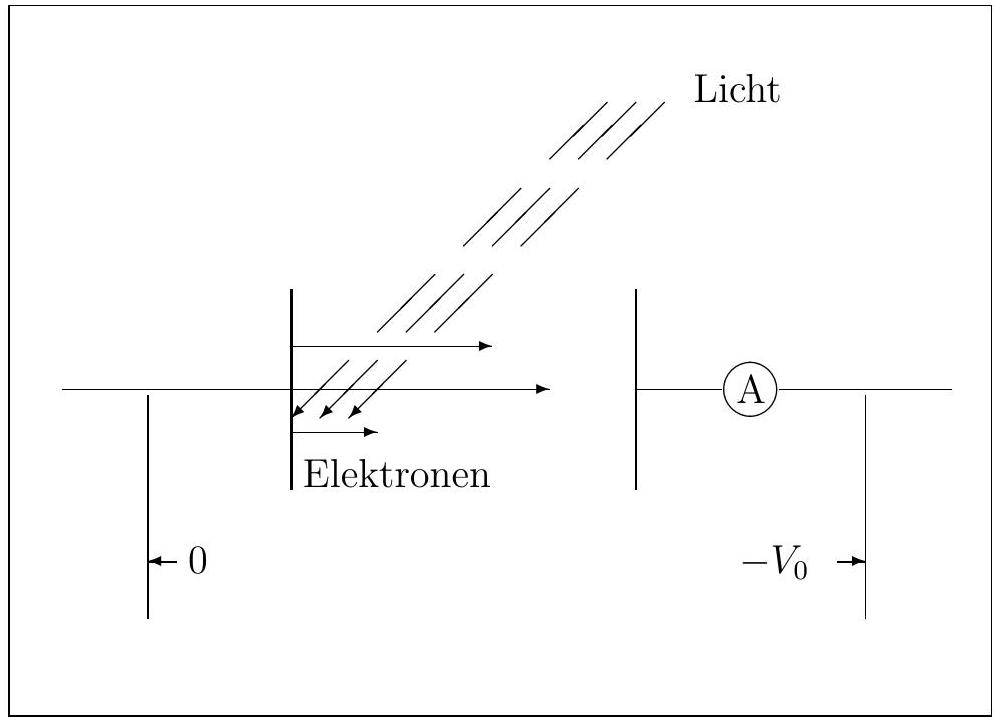
\includegraphics[scale=0.2, center]{2025_05_21_7e716008973ee1b5e8beg-05}

Dabei stellt sich folgendes heraus:

\begin{enumerate}
  \item Energie und Intensität
\end{enumerate}

Die Energie der Elektronen ist unabhängig von der Intensität des Lichtes, aber eine lineare Funktion seiner Frequenz $\omega$.\\
2. Austrittsarbeit

Elektronen werde nur emittiert, falls die Frequenz des Lichtes oberhalb einer bestimmten Schwelle liegt, welche man Austrittsarbeit nennt. Die Grenzfrequenz hängt von der Art des Metalles ab.\\
3. Photostrom

Die Größe des Photostromes durch (A), d.h. die Anzahl der Elektronen, ist proportional zur Intensität des Lichtes.

Dieser Effekt ist ihm Rahmen der klassischen Elektrodynamik nicht zu verstehen, die Energie der austretenden Elektronen sollte proportional zur Intensität $\left(\frac{\epsilon_{0}}{2} \vec{E}_{\omega}^{2}+\frac{1}{2 \mu_{0}} \vec{B}_{\omega}^{2}\right)$ des Lichtes sein.

\subsubsection*{Lichtquanten}
Für die Erklärung des Photoeffekts hat Einstein den Nobelpreis erhalten:\\
Das Licht besteht aus Teilchen (Quanten) mit der Energie $\hbar \omega$, falls das Licht die (Kreis-) Frequenz $\omega$ hat. Trifft ein solches Lichtquant auf die Metalloberfläche, so kann\\
es durch Zusammenstoß mit einem Elektron seine Energie auf dieses übertragen. Ist $A$ die "Austrittsarbeit" des Elektrons für das betreffende Metall, so gilt die Energiebilanz:

$$
\frac{1}{2} m_{e} \vec{v}_{e}{ }^{2}+A=\hbar \omega
$$

$m_{e}$ : Masse des Elektrons; $\vec{v}_{e}$ : Geschwindigkeit des Elektrons.\\
A hat die Größenordnung $\mathrm{eV}\left(1 \mathrm{eV}=1.602177 \ldots \cdot 10^{-19} \mathrm{~J}\right)$. Die Intensität des Lichtes ist proportional der Anzahl der Lichtquanten= "Photonen", d.h. je mehr Photonen auf das Metall fallen, desto mehr Elektronen werden herausgelöst.

\subsubsection*{Compton Effekt}
Dieser Effekt ist ein unmittelbarer Ausdruck der Teilchennatur des Lichtes: Läßt man Röntgenstrahlen senkrecht auf eine dünne Metallfolie fallen, so werden nach der klassischen Elektrodynamik die Elektronen in der Folie zu Schwingungen angeregt, deren Frequenz die gleiche wie die des Röntgenlichtes ist.\\
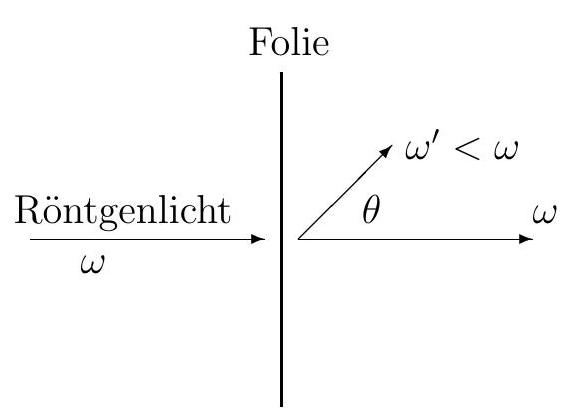
\includegraphics[scale=0.2, center]{2025_05_21_7e716008973ee1b5e8beg-06}

Die Elektronen sollten als schwingende Dipole Röntgenlicht gleicher Frequenz wieder abstrahlen, und zwar unabhängig von der Richtung $\theta$ (s. Skizze). Tatsächlich beobachtet man (Compton) folgendes: Die Frequenz des Lichtes hinter der Folie nimmt mit wachsendem $\theta$ ab!

\subsubsection*{Impuls von Photonen}
Wir überlegen uns zunächst, daß aus der speziellen Relativitätstheorie folgt, daß Photonen einen Impuls haben müßen:

$$
\text { relativistisch: } \quad E(\vec{p})=c \sqrt{\vec{p}^{2}+m^{2} c^{2}}
$$

Die Ruhemasse eines Photons (Lichtgeschwindigkeit) verschwindet, also gilt

$$
\text { Photon: } \quad E(\vec{p})=\hbar \omega=\hbar c|\vec{k}|=c|\vec{p}| .
$$

Es folgt dann $|\vec{p}|=\hbar|\vec{k}|$, und da der Ausbreitungsvektor $\vec{k}$ die gleiche Richtung wie $\vec{p}$ hat, ergibt sich

$$
\vec{p}_{P h o t o n} \equiv \vec{p}_{\gamma}=\hbar \vec{k}, \quad|\vec{k}|=2 \pi / \lambda
$$

\subsubsection*{Streuung von Photonen an Elektronen}
Man betrachte nun den Compton-Prozeß als elastischen Stoß zwischen Photonen und Elektronen. Die Elektronen befinden sich vor dem Stoß in Ruhe.

Ist nun $\vec{p}_{\gamma}$ der Impuls des Photons ( $\gamma$-Quants) vor dem Stoß mit dem Elektron, $\vec{p}_{\gamma}{ }^{\prime}$ sein Impuls nach dem Stoß und $\overrightarrow{p_{e}{ }^{\prime}}$ der Impuls des Elektrons nach dem Stoß, so lauten Energie- und Impulssatz:

$$
\begin{aligned}
\hbar \omega+m_{e} c^{2} & =\hbar \omega^{\prime}+\left(m_{e}^{2} c^{4}+\left(\vec{p}_{e}^{\prime}\right)^{2} c^{2}\right)^{\frac{1}{2}} \\
\vec{p}_{\gamma} & =\vec{p}_{\gamma}^{\prime}+\vec{p}_{e}^{\prime} \\
m_{e} & : \text { Ruhemasse des Elektrons. }
\end{aligned}
$$

Aus der ersten Gleichung folgt:

$$
\begin{aligned}
m_{e}^{2} c^{4}+\left(\vec{p}_{e}^{\prime}\right)^{2} c^{2} & =\left(\hbar \omega-\hbar \omega^{\prime}+m_{e} c^{2}\right)^{2} \\
& =\left(\hbar \omega-\hbar \omega^{\prime}\right)^{2}+2 m_{e} c^{2}\left(\hbar \omega-\hbar \omega^{\prime}\right)+m_{e}^{2} c^{4} \\
\left(\vec{p}_{e}^{\prime}\right)^{2} & =\frac{\hbar^{2} \omega^{2}}{c^{4}}-\frac{2 \hbar^{2} \omega \omega^{\prime}}{c^{4}}+\frac{\hbar^{2}\left(\omega^{\prime}\right)^{2}}{c^{4}}+\frac{2 m_{e}}{c^{2}}\left(\hbar \omega-\hbar \omega^{\prime}\right)
\end{aligned}
$$

Andererseits ergibt der Impulssatz:

$$
\begin{aligned}
\left(\vec{p}_{e}^{\prime}\right)^{2}=\left(\vec{p}_{\gamma}-\vec{p}_{\gamma}^{\prime}\right)^{2} & =\left(\hbar \vec{k}-\hbar \vec{k}^{\prime}\right)^{2} \\
& =\frac{\hbar^{2} \omega^{2}}{c^{2}}+\frac{\hbar^{2}\left(\omega^{\prime}\right)^{2}}{c^{2}}-2 \frac{\hbar \omega}{c} \frac{\hbar \omega^{\prime}}{c} \cos \theta
\end{aligned}
$$

Einsetzen führt zu

$$
\begin{aligned}
-2 \frac{\hbar \omega}{c} \frac{\hbar \omega^{\prime}}{c} \cos \theta & =-\frac{2 \hbar^{2} \omega \omega^{\prime}}{c^{4}}+\frac{2 m_{e}}{c^{2}}\left(\hbar \omega-\hbar \omega^{\prime}\right) \\
\hbar \omega \omega^{\prime}(1-\cos \theta) & =m_{e} c^{2}\left(\omega-\omega^{\prime}\right)
\end{aligned}
$$

oder, mit $\lambda=2 \pi c / \omega$,

$$
\lambda^{\prime}-\lambda=\frac{2 \pi \hbar}{m_{e} c}(1-\cos \theta)
$$

d.h. die Wellenlänge des abgelenkten Lichtes ist um so größer, je größer der Streuwinkel $\theta$ wird. Das Licht hat also ganz eindeutig Teilcheneigenschaften (Impuls, Energie, etc.).

\subsubsection*{Compton-Wellenlänge}
Man kann das "Rückstoß"-Elektron in Koinzidenz mit dem Photon messen (Geiger, Bothe). Die Größe $\lambda_{c}(e)=\hbar / m_{e} c=3.861593 \ldots \cdot 10^{-13} m$ bezeichnet man als Comp-ton-Wellenlänge des Elektrons.

\subsubsection*{Materiewellen}
Für Licht gelten die fundamentalen Beziehungen

$$
E=\hbar \omega, \quad \vec{p}=\hbar \vec{k}
$$

zwischen Welleneigenschaften $(\omega, \vec{k})$ auf der einen und den Teilcheneigenschaften $(E, \vec{p})$ auf der anderen Seite.

\subsubsection*{Teilchen-Wellen Dualismus}
Dieses motiviert die Hypothese (de Broglie), dass man umgekehrt auch Teilchen Welleneigenschaften zuschreiben können, mit

$$
\begin{aligned}
& \omega=\frac{1}{\hbar} E, \quad \vec{k}=\frac{1}{\hbar} \vec{p} \\
& E=\frac{\vec{p}^{2}}{2 m} \quad \text { oder } \quad E=c\left(\vec{p}^{2}+m^{2} c^{2}\right)^{1 / 2}
\end{aligned}
$$

\subsubsection*{de Broglie Wellenlänge}
Wir betrachten Elektron, welche aus der Ruhe auf die Geschwindigkeit $\vec{v}=\vec{p} / m$ gebracht werden, indem man sie eine Potentialdifferenz $U$ durchlaufen läßt. Nach dem Energiesatz gilt

$$
\frac{\vec{p}^{2}}{2 m_{e}}=e U, \quad \frac{1}{2 m_{e}}\left(\frac{2 \pi}{\lambda}\right)^{2} \hbar^{2}=e U
$$

wobei wir $\vec{p}=\hbar \vec{k}$ und $|\vec{k}|=\frac{2 \pi}{\lambda}$ verwendet haben.

$$
\begin{aligned}
\lambda_{e} & =\frac{2 \pi \hbar}{\left(2 m_{e} e U\right)^{\frac{1}{2}}} \\
& \approx\left(\frac{150}{U}\right)^{\frac{1}{2}} \text{\AA}, \quad U \text { in Volt }
\end{aligned}
$$

Die 'de Broglie'-Wellenlänge $\lambda_{e}$ der Elektronen ist also eine Funktion der durchlaufenen Spannung $U$. Bei $U=10^{2}, 10^{3}$ Volt, liegt $\lambda_{e}$ in der Größenordnung von Röntgenstrahlen. Experimente mit Elektronenstrahlen (analog zu den Röntgenspektrometern mit Hilfe von Kristallen als Beugungsgittern) haben ergeben, daß man Elektronen (und ebenso anderen atomaren Teilchen) Welleneigenschaften zuschreiben muß: man hat z.B. Interferenzen, Beugungserscheinungen etc. beobachtet. Da $\lambda \sim(1 / m)^{1 / 2}$, so spielt der Wellenaspekt bei makroskopischen Massen keine Rolle.

\subsubsection*{Bohr'sche Atommodell}
Streuversuche mit $\alpha$ - Teilchen und Atomen (Geiger, Marsden u.a.) hatten folgendes Atommodell (Rutherford) nahegelegt:

Die Atome bestehen aus einem nahezu punktförmigen positiven Kern (Radien $\leq 10^{-15} \mathrm{~m}$ ), um den die Elektronen in relativ weitem Abstand (Radius ca. $10^{-10} \mathrm{~m}$ ) "kreisen".

\subsubsection*{Atome sind klassisch instabil}
Das klassische AtomeModell kann die Streuexperimente gut erklären (Rutherford'sche Streuformel), führte aber zu prinzipiellen Schwierigkeiten bei den Spektren: Beschleunigte Ladungen strahlen nach der Elektrodynamik elektromagnetische Strahlung ab, deren Intensität proportional zum Quadrat der Beschleunigung ist. Die "kreisenden" Elektronen müßten also ständig strahlen und in ca. $10^{-10}$ sek in den Kern "fallen"; d.h. die Atome wären demnach instabil.

Einen phänomenologischen Ausweg aus dieser Schwierigkeit fand Bohr für wasserstoffartige Atome mit zwei Postulaten.

\subsubsection*{Interferierende Materiewellen}
Wir nehmen an, daß sich die Elektronen als selbstinterferierende Materiewellen auf einer Kreisbahn mit dem Radius $r_{n}$ um den Kern bewegt. Die Winkelabhängigkeit der Wellenfunktion des Elektrons ist dann

$$
\sim \mathrm{e}^{i k\left(r_{n} \varphi\right)},
$$

wobei $k=2 \pi / \lambda$ der (noch zu bestimmende) Wellenvektor des Elektron ist. Die Wellenfunktion muss als Funktion des Winkels $\varphi$ eindeutig sein, also

$$
k r_{n} 2 \pi=n 2 \pi, \quad r_{n}=\frac{n}{k}
$$

Für eine feste Quantenzahl $n$ ist der Wellenvektor $k$ dadurch bestimmt, dass durch ihn die Gesamtenergie des umlaufenden Elektrons,

$$
E=\frac{p^{2}}{2 m_{e}}-\frac{Z e^{2}}{4 \pi \epsilon_{0} r_{n}}=\frac{\hbar^{2} k^{2}}{2 m_{e}}-\frac{Z e^{2} k}{4 \pi \epsilon_{0} n}
$$

minimal wird (das entspricht einem Gleichgewicht der mechanischen Kräfte), $Z$ ist dabei die Kernladungszahl:

$$
\frac{\partial E(k)}{\partial k}=\frac{\hbar^{2} k}{m_{e}}-\frac{Z e^{2}}{4 \pi \epsilon_{0} n}=0, \quad k=\frac{m_{e}}{\hbar^{2}} \frac{Z e^{2}}{4 \pi \epsilon_{0} n} .
$$

Setzen wir dieses Ergebnis in $E(k)$ ein, so erhalten wir:

$$
\begin{aligned}
r_{n} & =\frac{4 \pi \varepsilon_{0} n^{2} \hbar^{2}}{Z e^{2} m_{e}} \\
E_{n} & =-\frac{1}{2} m_{e} c^{2} \frac{(\alpha Z)^{2}}{n^{2}}, \quad \alpha=\frac{e^{2}}{4 \pi \varepsilon_{0} \hbar c} .
\end{aligned}
$$

Die vom Maßsystem unabhängige dimensionslose Sommerfeld'sche Feinstrukturkonstante $\alpha$ hat den Zahlenwert $1 /(137.035 \ldots)$.

\subsubsection*{Spektren}
Auf den Bahnen $r_{n}$ strahlt das Elektron keine Energie ab. Strahlung findet dagegen statt, falls das Elektron von einem Niveau $E_{n_{2}}$ zu einem Niveau $E_{n_{1}}$ "springt", und zwar wird dabei Licht mit der Frequenz $\omega=\left(E_{n_{2}}-E_{n_{1}}\right) / \hbar$ abgestrahlt.

Diese Annahme ergibt unmittelbar die Balmer'sche Formel für die Spektrallinien des Wasserstoff - Atoms:

$$
\omega_{1,2}=\frac{1}{\hbar} \frac{1}{2} m_{e} c^{2} \alpha^{2} Z^{2}\left(\frac{1}{n_{1}^{2}}-\frac{1}{n_{2}^{2}}\right)
$$

Die Postulate 1 und 2 sind nicht aus der Mechanik und Elektrodynamik begründbar. Erst die Existenz des Wirkungsquantums $\hbar$ macht die Stabilität der Atome möglich.\\
Man bezeichnet mit $a_{0} \equiv r_{1}(Z=1)$ den Bohr'schen Radius:

$$
a_{0}=\frac{4 \pi \varepsilon_{0} \hbar^{2}}{e^{2} m_{e}}=0.529177 \text{\AA}
$$










\pagebreak



\section{Die Schrödinger - Gleichung}



\begin{DEF}{QM-G25-01-01}{Wellen-Teilchen Dualität und Plansche Wirkungsquantum}
Die in A2 Quantenphysik diskutierten Phänomene zeigen, daß Wellen Teilcheneigenschaften haben, und umgekehrt. Dabei sind für freie Teilchen, bzw. Wellen, die Größen Energie $E(\vec{p})$ und Impuls $\vec{p}$ auf der Teilchenseite mit den Größen Kreisfrequenz $\omega(\vec{k})$ und Wellenvektor $\vec{k}$ auf der Wellenseite durch die fundamentalen Beziehungen
$$
E=\hbar \omega, \quad \vec{p}=\hbar \vec{k}
$$
verknüpft. Dabei ist
$$
\hbar=1.054572 \ldots \cdot 10^{-34} \mathrm{~J} \mathrm{~s}=6.582 \ldots \cdot 10^{-22} \mathrm{MeV} \mathrm{~s} .
$$
das Planck'sche Wirkungsquantum (Energie mal Zeit, mit $\hbar=h /(2 \pi))$.
\begin{enumerate}
  \item $E = \hbar \omega$: Dass Licht aus Energiequanten (Photonen) besteht, folgt u.\,a. aus den Eigenschaften der Hohlraumstrahlung sowie aus dem photoelektrischen Effekt.
  \item $\vec{p} = \hbar \vec{k}$: Die Verknüpfung von Impuls mit dem Wellenvektor kann aus dem Compton-Effekt abgeleitet werden.
\end{enumerate}
\end{DEF}



Ausgehend von dieser Einsicht läßt sich die Schrödinger-Gleichung ableiten, was wir im Folgenden tun werden.



\subsection{Wellenpakete}


Wellen werden (wie in der Optik) in der Quantenmechanik mittels komplexer Zahlen beschrieben.



\subsubsection*{Ebene Wellen}


\begin{DEF}{QM-G25-02-01}{Ebene Wellen}
Ebene Wellen $\psi_{\mathbf{k}}(\vec{x}, t)$ sind wie in der Elektrodynamik durch
$$
\begin{aligned}
\psi_{\mathbf{k}}(\vec{x}, t) & =A(\vec{k}) e^{-i(\omega(\vec{k}) t-\vec{k} \cdot \vec{x})} \\
A(\vec{k}) & : \text { Amplitude } \\
\omega t-\vec{k} \cdot \vec{x} & : \text { Phase }
\end{aligned}
$$
definiert. Falls $|A|=\left[(\Re e A)^{2}+(\Im m A)^{2}\right]^{\frac{1}{2}} \neq 0$, so ist die Welle überall im Raum vorhanden.
\end{DEF}



\subsubsection*{Wellenpakete}

\begin{DEF}{QM-G25-02-02}{Wellenpakete}
Räumlich begrenzte Wellenzüge, sog. Wellenpakete, entstehen durch Überlagerung von ebenen Wellen mit verschiedenen $\vec{k}$ und $\omega(\vec{k})$.
\end{DEF}

\subsubsection*{Überlagerung zweier ebenen Wellen}

Als einfaches Beispiel für ein Wellenpaket betrachten wir die Überlagerung zweier ebenen Wellen.



\begin{EXA}{QM-G25-02-03}{Überlagerung von zwei Wellen}
Seien $\psi_{\mathbf{k}_{\mathbf{1}}}(\vec{x}, t)$ und $\psi_{\mathbf{k}_{\mathbf{2}}}(\vec{x}, t)$ zwei ebene Wellen mit nur wenig verschiedenen Wellenvektoren $\vec{k}_{i}$. Wir nehmen an, daß $\vec{k}_{i}=\left(k_{i}, 0,0\right)$, die Ausbreitung also in $x_{1}$-Richtung stattfinde. Die Überlagerung (Superposition) der beiden Wellen ist
$$
\psi_{\bar{k}}(\vec{x}, t)=A_{1} e^{-i\left(\omega_{1} t-k_{1} x\right)}+A_{2} e^{-i\left(\omega_{2} t-k_{2} x\right)}
$$
wobei wir $\vec{x}=\left(x_{1}, x_{2}, x_{3}\right)=(x, y, z)$ verwendet haben. Es sei $A_{1}=A_{2}=A$. Ferner setzen wir:
$$
\begin{array}{cc}
\omega_{1}=\bar{\omega}+\Delta \omega \quad, & \omega_{2}=\bar{\omega}-\Delta \omega \\
k_{1}=\bar{k}+\Delta k & , \quad k_{2}=\bar{k}-\Delta k
\end{array}
$$
und erhalten
$$
\begin{aligned}
\psi_{\bar{k}}(\vec{x}, t) & =A\left[e^{-i[(\bar{\omega}+\Delta \omega) t-(\bar{k}+\Delta k) x]}+e^{-i[(\bar{\omega}-\Delta \omega) t-(\bar{k}-\Delta k) x]}\right] \\
& =A\left[e^{-i(t \Delta \omega-x \Delta k)}+e^{+i(t \Delta \omega-x \Delta k)}\right] \cdot e^{-i(\bar{\omega} t-\bar{k} x)} \\
& =2 A \cos (t \Delta \omega-x \Delta k) e^{-i(\bar{\omega} t-\bar{k} x)}
\end{aligned}
$$
Durch Superposition der ebenen Wellen $\psi_{\mathbf{k}_{\mathbf{1}}}, \psi_{\mathbf{k}_{\mathbf{2}}}$ ensteht ein Wellenzug mit der mittleren Frequenz $\bar{\omega}$, dem Wellenvektor $\bar{k}$ und der "modulierten" Amplitude $\tilde{A}=2 A \cos (t \Delta \omega-$ $x \Delta k$ ). Die neue Amplitude $\tilde{A}$ ist eine Funktion von $\vec{x}$ und $t$. Sie ist maximal für
$$
t \Delta \omega-x \Delta k=n \pi, \quad n=0, \pm 1, \cdots
$$
und verschwindet für
$$
t \Delta \omega-x \Delta k=(2 n+1) \frac{\pi}{2}, \quad n=0, \pm 1 \cdots
$$
\end{EXA}

\subsubsection*{Gruppengeschwindigkeit}

\begin{EXA}{QM-G25-02-05}{Gruppengeschwindigkeit von Überlagerung zweier Wellen}
Die "Bewegung" des durch $t \Delta \omega-x \Delta k=0$ gegebenen Maximums von $\tilde{A}$ ist durch
$$
\tilde{x}(t)=\frac{\Delta \omega}{\Delta k} t
$$
charakterisiert. Im Limes $\Delta k \rightarrow 0$ wird daraus
$$
\tilde{x}(t)=\frac{\partial \omega}{\partial k} t,
$$
oder, im 3 - dimensionalen Fall,
$$
\overline{\vec{x}}=\left(\operatorname{grad}_{\mathbf{k}} \omega(\vec{k})\right) t
$$
Das Maximum der superponierten Welle wandert also mit der Geschwindigkeit
$$
\vec{v}_{g}:=\operatorname{grad}_{\mathrm{k}} \omega(\vec{k})
$$
durch den Raum. Man bezeichnet diese Geschwindigkeit als Gruppengeschwindigkeit des Wellenzuges (Wellenpaketes).
Wegen $E=\hbar \omega, \vec{p}=\hbar \vec{k}$ gilt
$$
\vec{v}_{g}=\operatorname{grad}_{\mathbf{p}} E(\vec{p})=\vec{v}
$$
Die Gruppengeschwindigkeit eines Wellenpaketes ist gleich der "mechanischen" Geschwindigkeit der zugeordneten Teilchen.
\end{EXA}



\begin{CONC}{QM-G25-02-04}{$E(\vec{p})=\vec{p}^{2} /(2 m)$}
Man betrachte z.B. 
$$E(\vec{p})=\vec{p}^{2} /(2 m)$$ 
Dies ist ein wichtiger Zusammenhang zwischen Wellen- und Teilcheneigenschaften.
\end{CONC}


\subsubsection*{Phasengeschwindigkeit}


\begin{DEF}{QM-G25-02-06}{Phasengeschwindigkeit eine Wellenphase}
Die Ausbreitung der Wellenphase $\bar{\omega} t-\bar{k} x$ ist durch $\bar{\omega} t-\bar{k} x=$ const. charakterisiert und durch 
$$v_{\text {phase }}=\bar{\omega} / \bar{k}$$ 
gegeben. Man bezeichnet sie mit Phasengeschwindigkeit. Wie wir von den Radiowellen wissen, findet die Übertragung der "Information" via der Modulation der Amplitude statt, die Information breitet sich also mit der Gruppengeschwindigkeit $\vec{v}_{g}$ aus.
\end{DEF}

\subsubsection*{Allgemeines Wellenpaket}


\begin{DEF}{QM-G25-02-07}{Allgemeines Wellenpaket}
Im allgemeinen enthält ein Wellenzug (Wellenpaket) unendlich viele Frequenzen,
$$
\psi(\vec{x}, t)=\int_{-\infty}^{+\infty} \int_{-\infty}^{+\infty} \int_{-\infty}^{+\infty} d^{3} k g(\vec{k}) e^{-i(\omega(\vec{k}) t-\vec{k} \cdot \vec{x})}
$$
was einer Fourier-Zerlegung mit (komplexen) Fourier-Komponenten $g(\vec{k})$ entspricht. Letzter bestimmen, mit welchem Gewicht einzelne ebenen Wellen $\psi_{\mathbf{k}}(\vec{x}, t)$ an dem Wellenpaket beteiligt sind.
\end{DEF}


\subsubsection*{Gauß'sche Wellenpakete}


Für eine Motivation der Unschärfe-Relation betrachten wir hier den eindimensionallen Fall.



\subsubsection*{Gauß'sches Wellenpaket für den eindimensionalen Fall}


\begin{EXA}{QM-G25-02-08}{Gauß'sches Wellenpaket für den eindimensionalen Fall}
Die Funktion
$$
g(k)=e^{-\alpha\left(k-k_{o}\right)^{2}}, \quad \alpha>0
$$
beschreibt eine Gauß'sche Verteilung, die bei $k=k_{0}$ konzentriert ist. Die Breite $\sigma$ der Verteilung ist durch den Parameter $\alpha=1 /\left(2 \sigma^{2}\right)$ charakterisiert. Das Wellenpaket lautet
$$
\psi(x, t)=\int_{-\infty}^{+\infty} d k e^{-\alpha\left(k-k_{0}\right)^{2}} e^{-i(\omega(k) t-k x)}
$$
Die klasssiche $E=p^{2} /(2 m)$ und die relativistische $E^{2}=c^{2} p^{2}+m^{2} c^{4}$ Energie-Impuls Beziehungen für freie Teilchen führen jeweils zu
$$
\begin{aligned}
\omega & =\frac{1}{\hbar} \frac{1}{2 m}(\hbar k)^{2}=\frac{\hbar}{2 m} k^{2} \\
\omega & =\frac{1}{\hbar} c \sqrt{\left.(\hbar k)^{2}+m^{2} c^{2}\right)}=c\left(k^{2}+\left(\frac{m c}{\hbar}\right)^{2}\right)^{\frac{1}{2}}
\end{aligned}
$$
wobei wir $E=\hbar \omega$ und $p=\hbar k$ verwendet haben. Allgemein ist Entwicklung von $\omega(k)$ um $k=k_{0}$
$$
\omega(k)=\omega\left(k_{0}\right)+\left.\frac{d \omega}{d k}\right|_{k=k_{0}}\left(k-k_{0}\right)+\left.\frac{1}{2} \frac{d^{2} \omega}{d k^{2}}\right|_{k=k_{0}}\left(k-k_{0}\right)^{2}+\cdots
$$
Für das Gauß'sche Wellenpaket ist die Verteilung $\omega(k)$ um $k=k_{0}$ konzentriert, wir können also die Entwicklung nach dem zweiten Glied abbrechen (für $\omega=\frac{\hbar}{2 m} k^{2}$ wäre dies exakt).
$$
\begin{array}{rlrl}
\left.\frac{d \omega}{d k}\right|_{k=k_{0}} & =v_{g} & & \text { (Gruppengeschwindigkeit) } \\
\left.\frac{1}{2} \frac{d^{2} \omega}{d k^{2}}\right|_{k=k_{0}} & \equiv \beta & \left(\rightarrow \frac{\hbar}{2 m} \quad \text { für } \quad \omega=\frac{\hbar}{2 m} k^{2}\right)
\end{array}
$$
Für das Wellenpaket ergibt sich damit
$$
\psi(x, t)=\int_{-\infty}^{+\infty} d k e^{-\alpha\left(k-k_{0}\right)^{2}} e^{-i\left[\omega\left(k_{0}\right) t+v_{g}\left(k-k_{0}\right) t+\beta\left(k-k_{0}\right)^{2} t-k x\right]}
$$
Wir führen die Variablen-Substitution $\tilde{k}=k-k_{0}$ durch:
$$
\psi(x, t)=e^{-i\left(\omega\left(k_{0}\right) t-k_{0} x\right)} \int_{-\infty}^{+\infty} d \tilde{k} e^{-\alpha \tilde{k}^{2}-i \beta t \tilde{k}^{2}} e^{i \tilde{k}\left(x-v_{g} t\right)}
$$
Das Gauss'sche Integral ergibt (Übungen)
$$
\int_{-\infty}^{+\infty} d y e^{-\gamma y^{2}} e^{-i u y}=\sqrt{\frac{\pi}{\gamma}} \exp \left(-\frac{1}{4 \gamma} u^{2}\right)
$$

Diese Formel gilt auch für komplexe $\gamma$, falls $\Re e \gamma>0$, so daß wir insgesamt zu folgendem Resultat gelangen:
$$
\psi(x, t)=\left(\frac{\pi}{\alpha+i \beta t}\right)^{\frac{1}{2}} e^{-\frac{1}{4(\alpha+i \beta t)}\left(x-v_{g} t\right)^{2}} e^{-i\left(\omega\left(k_{0}\right) t-k_{0} x\right)}
$$
Das Wellenpaket $\psi(x, t)$ ist eine Welle mit der Phase $\omega\left(k_{0}\right) t-k_{0} x$ und der ortsabhängigen Amplitude
$$
\begin{aligned}
A_{G}(x, t) & =\left(\frac{\pi}{\alpha+i \beta t}\right)^{\frac{1}{2}} e^{-\frac{1}{4(\alpha+i \beta t)}\left(x-v_{g} t\right)^{2}} \\
\left|A_{G}(x, t)\right|^{2}=A_{G} A_{G}^{*} & =\left(\frac{\pi^{2}}{\alpha^{2}+\beta^{2} t^{2}}\right)^{\frac{1}{2}} e^{-\frac{\alpha\left(x-v_{g} t\right)^{2}}{2\left(\alpha^{2}+\beta^{2} t^{2}\right)}}
\end{aligned}
$$
Die Intensität $|\psi(x, t)|^{2}=\left|A_{G}\right|^{2}$ ist also wieder eine Gauß'sche Verteilung. Mit $\sigma^{2}=$ $\left(\alpha^{2}+\beta^{2} t^{2}\right)$ wächst die Varianz $\sigma$ mit der Zeit.
\end{EXA}



\subsubsection*{Gruppengeschwindingkeit}


\begin{CONC}{QM-G25-02-09}{Rolle der Gruppengeschwindigkeit}
Bei festem $t$ ist $|\psi(x, t)|^{2}$ maximal, falls $x=v_{g} t$, d.h. dort, wo sich nach der klassischen Mechanik $(x(t)=v t)$ das Teilchen befinden sollte. Das Maximum wandert mit der Geschwindigkeit $v_{g}$.
\end{CONC}

\subsubsection*{Unschärfe-Relation}


\begin{CONC}{QM-G25-02-10}{Herleitung der Unschärferelation für Gauß'sche Wellenpaket}
Für $t=0$ ist
$$
|\psi(x, 0)|^{2}=\frac{\pi}{\alpha} e^{-\frac{x^{2}}{2 \alpha}} \equiv \frac{\pi}{\alpha} e^{-\frac{x^{2}}{2 \sigma_{x}^{2}}}
$$
was wir mit
$$
|g(k)|^{2}=e^{-2 \alpha\left(k-k_{0}\right)^{2}} \equiv e^{-\frac{\left(k-k_{0}\right)^{2}}{2 \sigma_{k}^{2}}}
$$
in Verbindung setzten können. Wir definieren
$$
\begin{aligned}
& \delta x(0)=\sqrt{2 \alpha}: \begin{array}{l}
\text { Breite des Wellenpaketes im Ortsraum zur } \\
\text { Zeit } \mathrm{t}=0
\end{array} \\
& \delta k:=1 / \sqrt{2 \alpha}: \begin{array}{l}
\text { Breite des Gauß'schen Wellenpaketes } \\
\text { im } k \text {-Raum }
\end{array}
\end{aligned}
$$
denn, z.B. falls $k-k_{0}=\delta k$, so ist $|g(k)|^{2}$ auf den $e$ - ten Teil abgefallen. Zwischen $\delta x(0)$ und $\delta k$ gilt die Beziehung
$$
\delta k \delta x(0)=1
$$
Je schmaler also ein Wellenpaket im $k$ - Raum ist (d.h. je schmaler die Spektrallinie ist), um so breiter ist das Wellenpaket im Ortsraum und umgekehrt (Der Wert on der rechten Seite hängt von der Definition der Unschärfe ab. Verwendet man die Standardabweisungen $\sigma_x=\sqrt{\alpha}$ und $\sigma_k=1 /(2 \sqrt{\alpha})$, so erhält man $\sigma_x \sigma_k=1 / 2$.). Mit $p=\hbar k$ folgt schlussendlich
$$
\delta p \delta x(0)=\hbar
$$
Je genauer man also den Impuls eines Teilchens kennt ("Unschärfe" $\delta p$ ), desto weniger genau kann man seinen Ort $x$ angeben ("Unschärfe" $\delta x$ ). Das Produkt der Unschärfen ist durch $\hbar$ gegeben was die Heisenberg'sche Unschärferelation definiert.
\end{CONC}

\subsubsection*{Born'sche Interpretation}


\begin{CONC}{QM-G25-02-11}{Born'sche Interpretation der Unschärferelation}
Die Unschärferelation gilt - wie wir sehen werden - für beliebige Wellenpakete. Sie bedeutet, daß die Wellenfunktion nicht die Materieverteilung eines Teilchens beschreiben kann, denn erfahrungsgemäß zerfließen Elektronen, Protonen und Atome nicht.

Nach Born ist $|\psi(x, t)|^{2}$ vielmehr als Wahrscheinlichkeitsdichte zu interpretieren, wie wir weiter unten noch ausführlicher diskutieren werden.
\end{CONC}








\subsection{Schrödinger - Gleichung}



\subsubsection{Herleitung für freie Teilchen}



\begin{CONC}{QM-G25-03-01}{Herleitung der Schrödinger-Gleichung für freie Teilchen für ebene Welle}
Mit $E=\hbar \omega$ und $\vec{p}=\hbar \vec{k}$ nimmt die ebene Welle $\psi_{\mathbf{k}}(\vec{x}, t)=A e^{-i(\omega t-\vec{k} \cdot \vec{x})}$ die Form
$$
\psi_{\mathbf{p}}(\vec{x}, t)=A e^{-\frac{i}{\hbar}(E t-\vec{p} \cdot \vec{x})}
$$
an. Für ein nichtrelativistisches Teilchen hat man $E=\frac{1}{2 m} \vec{p}^{2}$. Mit
$$
\partial_{t} \psi_{\mathbf{p}}(\vec{x}, t)=-\frac{i}{\hbar} E \psi_{\mathbf{p}}(\vec{x}, t)
$$
und
$$
\frac{\partial}{\partial x_{j}} \psi_{\mathbf{p}}(\vec{x}, t) \equiv \partial_{j} \psi_{\mathbf{p}}(\vec{x}, t)=\frac{i}{\hbar} p_{j} \psi_{\mathbf{p}}(\vec{x}, t)
$$
folgt
$$
\begin{aligned}
\Delta \psi_{\mathbf{p}}(\vec{x}, t) \equiv\left(\partial_{1}^{2}+\partial_{2}^{2}+\partial_{3}^{2}\right) \psi_{\mathbf{p}}(\vec{x}, t) & =-\frac{1}{\hbar^{2}} \vec{p}^{2} \psi_{\mathbf{p}}(\vec{x}, t) \\
& =-\frac{2 m}{\hbar^{2}} E \psi_{\mathbf{p}}(\vec{x}, t)
\end{aligned}
$$
Also genügt $\psi_{\mathbf{p}}(\vec{x}, t)$ der (partiellen) Differentialgleichung
$$
i \hbar \partial_{t} \psi_{\mathbf{p}}(\vec{x}, t)=-\frac{\hbar^{2}}{2 m_{e}} \Delta \psi_{\mathbf{p}}(\vec{x}, t)
$$
Analog gilt für das Integral
$$
\psi(\vec{x}, t)=(2 \pi \hbar)^{-\frac{3}{2}} \int_{-\infty}^{+\infty} \widetilde{\psi}(\vec{p}) e^{-\frac{i}{\hbar}\left(\frac{\vec{p}^{2}}{2 m} t-\vec{p} \cdot \vec{x}\right)} d^{3} p
$$
die Schrödinger-Gleichung für freie Teilchen:
$$
i \hbar \partial_{t} \psi(\vec{x}, t)=-\frac{\hbar^{2}}{2 m_{e}} \Delta \psi(\vec{x}, t)
$$
\end{CONC}

\subsubsection*{Superpositionsprinzip}


\begin{CONC}{QM-G25-03-02}{Schrödinger-Gleichung erfüllt Superpositionsprinzip}
Die Schrödinger-Gleichung ist eine lineare partielle Differentialgleichung in den Zeit- und Orts-koordinaten. Die Linearität trägt dem für die Quantentheorie fundamentalen Superpositionsprinzip Rechnung:

Beschreiben $\psi_{1}$ und $\psi_{2}$ zwei quantentheoretisch mögliche physikalische Zustände, so beschreibt auch die lineare Superpostion
$$
c_{1} \psi_{1}+c_{2} \psi_{2}, \quad c_{i} \in \mathcal{C}
$$
einen möglichen physikalischen Zustand.
\end{CONC}


\subsubsection*{Korrespondenzprinzip}


\begin{CONC}{QM-G25-03-03}{Korrespondenzprinzip mit Operatorzuweisung}
Man erhält die freie Schrödinger-Gleichung formal, indem man in der Beziehung $E=\frac{1}{2 m} \vec{p}^{2}$ folgende Zuordnungen macht:
$$
E \rightarrow i \hbar \partial_{t}, \quad p_{j} \rightarrow \mathbf{P}_{j}:=\frac{\hbar}{i} \partial_{j}
$$
sowie
$$
\frac{1}{2 m} \vec{p}^{2} \quad \rightarrow \quad \frac{1}{2 m} \overrightarrow{\mathbf{P}}^{2}=-\frac{\hbar^{2}}{2 m_{e}} \Delta \equiv \mathbf{H}_{0}
$$
Die Differential-Operatoren $i \hbar \partial_{t}$ und $\mathbf{H}_{0}$ sind auf die Wellenfunktion $\psi(\vec{x}, t)$ anzuwenden. Aus $E=\frac{1}{2 m} \vec{p}^{2}$ folgt dann die freie Schrödinger-Gleichung:
$$
i \hbar \partial_{t} \psi(\vec{x}, t)=\mathbf{H}_{0} \psi(\vec{x}, t)=-\frac{\hbar^{2}}{2 m_{e}} \Delta \psi(\vec{x}, t)
$$
\end{CONC}



\subsubsection{Teilchen in äußerem Potential}



\begin{CONC}{QM-G25-04-01}{Korrespondenzprinzip mit Operatorzuweisung für ortsabhängiges Potential}
Ein klassisches Teilchen, das sich in einem Potential $V(\vec{x})$ (unabhängig von $t$ und $\vec{p}$) befindet, besitzt die Gesamtenergie $E=\frac{1}{2 m} \vec{p}^{2}+V(\vec{x})$. Die Verallgemeinerung des obigen freien Falles ist dann
$$
E \rightarrow \mathbf{H}:=\mathbf{H}_{0}+V(\vec{x})=-\frac{\hbar^{2}}{2 m_{e}} \Delta+V(\vec{x})
$$
mit dem Konventionsfaktor $(2 \pi \hbar)^{-3/2}$ erhält man schließlich die zugehörige Schrödinger-Gleichung:
$$
i \hbar \partial_{t} \psi(\vec{x}, t)=\mathbf{H} \psi(\vec{x}, t)=-\frac{\hbar^{2}}{2 m_{e}} \Delta \psi(\vec{x}, t)+V(\vec{x}) \psi(\vec{x}, t)
$$
Die Schrödinger-Gleichung mit Potential ist eine lineare Differentialgleichung, also gilt auch hier das Superpositionsprinzip. Umgekehrt folgt die Linearität der SchrödingerGleichung für ein Teilchen mit Wechselwirkung aus der Forderung nach Gültigkeit des Superpositionsprinzipes für Wellenfunktionen.
\end{CONC}



\begin{REM}{QM-G25-04-02}{Superposition nicht i.A. für Hamilton'sche Bewegungsgleichung}
Man beachte, daß das Superpositionsprinzip in der Mechanik i.allg. nicht gilt, da die (Hamilton'schen) Bewegungsgleichungen i.allg. nicht linear sind.
\end{REM}



\subsubsection*{Plausibilitätsbetrachtung}


\begin{EXA}{QM-G25-04-03}{Plausibilitätsbetrachtung für Schrödinger-Gleichung für äußeres Potential}
Die Schrödinger-Gleichung
$$
i \hbar \partial_{t} \psi(\vec{x}, t)=\left(-\frac{\hbar^{2}}{2 m_{e}} \Delta+V(\vec{x})\right) \psi(\vec{x}, t)
$$
für ein Teilchen in einem klassischen äußeren Potential $V(\vec{x})$ kann man sich folgendermaßen plausibel machen:

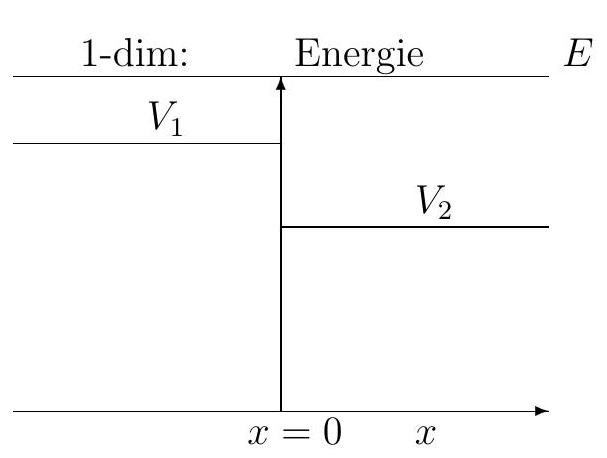
\includegraphics[scale=0.2, center]{2025_05_21_11b1754c718f6fcf84f8g-08}

Teilchen der Energie $E$ befinden sich für $x<0$ in einem Potential $V_{1}>0$ und für $x>0$ in $V_{2} \geq 0, V_{1}>V_{2}$.

Z.B. $x<0$ : Elektronen in einem Leiter $x>0$ : im leeren Raum

In beiden Fällen, $j=1,2$, sind den Teilchenstrahlen ebene Wellen zugeordnet:
$$
\begin{aligned}
\psi_{j} & =A_{j} e^{-\frac{i}{\hbar}\left(E t-p_{j} x\right)}, \quad p_{j}=\left[2 m\left(E-V_{j}\right)\right]^{\frac{1}{2}} \\
E & =\frac{1}{2 m} p_{1}^{2}+V_{1}=\frac{1}{2 m} p_{2}^{2}+V_{2}
\end{aligned}
$$
Für $x<0$ bzw. $x>0$ gelten jeweils die Gleichungen
$$
\begin{aligned}
i \hbar \partial_{t} \psi_{1}(x, t) & =-\frac{\hbar^{2}}{2 m} \frac{d^{2}}{d x^{2}} \psi_{1}(x, t)+V_{1} \psi_{1}(x, t) \\
i \hbar \partial_{t} \psi_{2}(x, t) & =-\frac{\hbar^{2}}{2 m} \frac{d^{2}}{d x^{2}} \psi_{2}(x, t)+V_{2} \psi_{2}(x, t)
\end{aligned}
$$
Hat man nun $n$ verschiedene Gebiete mit $V_{\nu}=$ const. $\nu=1, \ldots n$, mit $V_{\nu_{1}} \neq V_{\nu_{2}}$, so erhält man für jedes $\nu$ eine entsprechende Gleichung wie oben. Eine naheliegende (aber\\
nicht zwingende) Verallgemeinerung für kontinuierliche $V(x)$ ist dann:
$$
i \hbar \partial_{t} \psi(x, t)=\left(-\frac{\hbar^{2}}{2 m} \frac{d^{2}}{d x^{2}}+V(\vec{x})\right) \psi(x, t)
$$
Die eigentliche Bestätigung der Schrödinger - Gleichung erhält man durch Vergleich mit experimentellen Resultaten.
\end{EXA}





\subsubsection{Operatoren}



\begin{REM}{QM-G25-05-01}{Charakterisierung von Operatoren}
Operatoren sind nichts anderes als Vorschriften, wie Elemente einer vorgegebenen Menge bestimmte Elemente einer anderen Menge (die gleich der ursprünglichen sein kann) zugeordnet werden. Ein anderer Name für derartige Vorschriften ist Abbildung.
\end{REM}

\subsubsection*{Matrizen}


Es sei $\left(\mathbf{e}_{\mathbf{1}}, \mathbf{e}_{\mathbf{2}}\right)$ eine feste Basis im $\mathbb{R}^{2}$. Man hat dann
$$
\vec{x}=x_{1} \mathbf{e}_{\mathbf{1}}+x_{2} \mathbf{e}_{\mathbf{2}} \quad \leftrightarrow \quad\binom{x_{1}}{x_{2}}=\mathbf{x}
$$

Jede Matrix
$$
\mathbf{A}=\left(\begin{array}{ll}
a_{11} & a_{12} \\
a_{21} & a_{22}
\end{array}\right)
$$
definiert eindeutig eine Abbildung $\mathbb{R}^{2} \rightarrow \mathbb{R}^{2}$ durch, die Vorschrift
$$
\mathbf{x} \quad \rightarrow \quad \mathbf{x}_{\mathbf{A}}=\mathbf{A} \cdot \mathbf{x} \quad \text { für alle } \mathbf{x} \in \mathbb{R}^{2} .
$$
Hier ist A ein Matrix - Operator.


\subsubsection*{Beispiele für Operatoren}


\begin{DEF}{QM-G25-05-02}{Multiplikations-,Differential-,Konjugation-Operator auf $L^2(\R,\C)$}
Sei
\[
\mathcal{F} := \left\{ f_1(x), \dotsc, f_n(x) \,\middle|\, f_\nu : \mathbb{R} \to \mathbb{C}, \; \int_{\mathbb{R}} |f_\nu(x)|^2 \, dx < \infty \right\}
\]
eine Menge quadratintegrierbarer komplexwertiger Funktionen auf der reellen Achse. Auf diesem Raum können verschiedene Operatoren definiert werden:

\begin{enumerate}
  \item \textbf{Multiplikationsoperator:}

  Die Vorschrift
  \[
  f_\nu(x) \mapsto x^2 f_\nu(x)
  \]
  definiert den Multiplikationsoperator $M_{x^2}$ durch
  \[
  M_{x^2} f_\nu(x) := x^2 f_\nu(x).
  \]
  Beachte: Im Allgemeinen gilt $x^2 f_\nu(x) \notin \mathcal{F}$, da die Multiplikation mit $x^2$ die Quadratintegrabilität verletzen kann. Der Operator $M_{x^2}$ ist also nur auf einem geeigneten Definitionsbereich $\mathcal{D}(M_{x^2}) \subset \mathcal{F}$ wohldefiniert.

  \item \textbf{Differentialoperator:}

  Die Vorschrift
  \[
  f_\nu(x) \mapsto \frac{d}{dx} f_\nu(x)
  \]
  definiert den Differentialoperator $D$ durch
  \[
  D f_\nu(x) := \frac{d}{dx} f_\nu(x).
  \]
  Voraussetzung ist $f_\nu \in C^1(\mathbb{R})$. Auch hier ist $D f_\nu(x)$ nicht notwendigerweise wieder in $\mathcal{F}$, sodass auch hier der Operator nur auf einem Teilraum $\mathcal{D}(D) \subset \mathcal{F} \cap C^1(\mathbb{R})$ wohldefiniert ist.

  \item \textbf{Komplexe Konjugation:}

  Die Vorschrift
  \[
  f_\nu(x) \mapsto f_\nu^*(x)
  \]
  definiert den (antilinearen) Operator $K$ durch
  \[
  K f_\nu(x) := f_\nu^*(x).
  \]
  Dieser ist auf ganz $\mathcal{F}$ wohldefiniert, da
  \[
  \int_{\mathbb{R}} |f_\nu^*(x)|^2 \, dx = \int_{\mathbb{R}} |f_\nu(x)|^2 \, dx < \infty.
  \]
  Der Operator $K$ ist involutiv ($K^2 = \operatorname{id}$) und normerhaltend bezüglich des Skalarprodukts im Hilbertraum $L^2(\mathbb{R})$:
  \[
  \langle Kf, Kg \rangle = \langle g, f \rangle.
  \]
  
\end{enumerate}
\end{DEF}

\textbf{Bemerkung:} Diese Beispiele zeigen, dass bei der Definition von Operatoren auf Funktionenräumen stets auf die Wahl des geeigneten Definitionsbereichs zu achten ist. In der Quantenmechanik sind viele dieser Operatoren unbeschränkt und erfordern eine sorgfältige funktionalanalytische Behandlung.


\subsubsection*{Anmerkungen}
Bei der Definition eines Operators ist es wesentlich, die zugehörigen Mengen anzugeben:

\begin{itemize}
  \item \textbf{Urbildmenge} = \emph{Definitionsbereich}
  \item \textbf{Bildmenge} = \emph{Wertebereich}
\end{itemize}

Ein Operator ist nur dann wohldefiniert, wenn er auf seinem Definitionsbereich angewendet werden kann und das Ergebnis im Zielraum (Wertebereich) liegt.

\vspace{1em}




Lineare Operatoren

\begin{DEF}{QM-G25-05-03}{Lineare Operatoren}
Ein Operator $A$ heißt \emph{linear}, wenn für alle skalaren Kombinationen seiner Argumente gilt:
\[
A(\lambda_1 f_1 + \lambda_2 f_2) = \lambda_1 A(f_1) + \lambda_2 A(f_2)
\]
Dies gilt etwa für den Matrixoperator $\mathbf{A}$ auf $\mathbb{R}^2$:
\[
\mathbf{x}^{(1)}, \mathbf{x}^{(2)} \in \mathbb{R}^{2}, \quad \lambda_1, \lambda_2 \in \mathbb{R} \Rightarrow
\]
\[
\mathbf{A}(\lambda_1 \mathbf{x}^{(1)} + \lambda_2 \mathbf{x}^{(2)}) = \lambda_1 \mathbf{A} \mathbf{x}^{(1)} + \lambda_2 \mathbf{A} \mathbf{x}^{(2)}
\]

Auch der Differentialoperator ist linear:
\[
f_1, f_2 \in C^1(\mathbb{R}), \quad \lambda_1, \lambda_2 \in \mathbb{C}
\Rightarrow
\frac{d}{dx}(\lambda_1 f_1 + \lambda_2 f_2)
= \lambda_1 \frac{d}{dx} f_1 + \lambda_2 \frac{d}{dx} f_2
\]
\end{DEF}

\vspace{1em}




Antilineare Operatoren


\begin{DEF}{QM-G25-05-04}{Antilineare Operatoren}
Ein Operator $K$ heißt \emph{antilinear}, wenn für alle komplexen Skalare gilt:
\[
K(\lambda_1 f_1 + \lambda_2 f_2) = \lambda_1^* K(f_1) + \lambda_2^* K(f_2)
\]
Dies ist z.B. der Fall für den Operator der \emph{komplexen Konjugation}:
\[
K f(x) := f^*(x)
\]
\end{DEF}


\vspace{1em}




Vertauschungsrelationen

\begin{CONC}{QM-G25-05-05}{Vertauschungsrelation von Operatoren}
Operatoren \emph{vertauschen im Allgemeinen nicht}. Seien $\mathbf{A}_1$, $\mathbf{A}_2$ zwei Matrizen, so gilt im Allgemeinen:
\[
\mathbf{A}_1 \mathbf{A}_2 \neq \mathbf{A}_2 \mathbf{A}_1
\]
Man definiert den \emph{Kommutator}:
\[
[\mathbf{A}_1, \mathbf{A}_2] := \mathbf{A}_1 \mathbf{A}_2 - \mathbf{A}_2 \mathbf{A}_1
\]
Ein anschauliches Beispiel:
\[
\frac{d}{dx}(x f(x)) = f(x) + x \frac{d}{dx} f(x)
\]
\[
\Rightarrow \left[ \frac{d}{dx}, x \right] := \frac{d}{dx} x - x \frac{d}{dx} = \mathbf{1}
\]
Dabei ist $\mathbf{1}$ der \emph{Identitätsoperator}.
\end{CONC}

\vspace{1em}



Skalarprodukt und Norm


\begin{DEF}{QM-G25-05-06}{Skalarprodukt und Norm in komplexwertigen Vektorraum}
In einem komplexwertigen Vektorraum $\mathbb{C}^N$ mit Vektoren
\[
\mathbf{x} = (x_1, \dots, x_N), \quad \mathbf{y} = (y_1, \dots, y_N)
\]
ist das \emph{Skalarprodukt} definiert durch:
\[
(\mathbf{x}, \mathbf{y}) := \sum_{i=1}^N x_i^* y_i
\]
Die zugehörige \emph{Norm} ist:
\[
\|\mathbf{x}\| = \sqrt{(\mathbf{x}, \mathbf{x})} = \sqrt{\sum_i |x_i|^2}
\]

Für eine Matrix $A \in \mathbb{C}^{N \times N}$ gilt:
\[
(\mathbf{x}, A \mathbf{y}) = \sum_{i,j} x_i^* A_{ij} y_j
\]
\end{DEF}





\subsubsection{Das Korrespondenzprinzip}


\subsubsection*{Ortsoperators}


\begin{DEF}{QM-G25-07-02}{Ortsoperator als linearer Multiplikation-Operator}
Der lineare Multiplikations-Operatore
$$
\mathbf{Q}_{j}: \quad \mathbf{Q}_{j} \psi=x_{j} \psi, \quad j=1,2,3
$$
wird Ortsoperator genannt.
\end{DEF}

\subsubsection*{Impulsoperator}


\begin{DEF}{QM-G25-07-03}{Impulsoperator als linearer Differential-Operator}
Der linearen Differential-Operator
$$
\mathbf{P}_{j}: \quad \mathbf{P}_{j} \psi=\frac{\hbar}{i} \partial_{j} \psi, \quad j=1,2,3
$$
wird Impulsoperator genannt.
\end{DEF}

\subsubsection*{Linearität des Schrödinger-Operators}


\begin{CONC}{QM-G25-07-04}{Schrödinger-Operator als Funktion von Orts- und Impulsoperator}
Der Schrödinger-Operator
$$
\mathbf{H}=-\frac{\hbar^{2}}{2 m_{e}} \Delta+V(\vec{x})
$$
ist ein linearer Operator im Raum der Wellenfunktionen $\psi(\vec{x}, t)$. Er ist mit
$$
\mathbf{H}=\mathbf{H}(\overrightarrow{\mathbf{P}}, \overrightarrow{\mathbf{Q}})=\frac{1}{2 m} \overrightarrow{\mathbf{P}}^{2}+V(\overrightarrow{\mathbf{Q}})
$$
eine Funktion des Orts- und des Impulsoperators.
\end{CONC}

\subsubsection*{Vertauschungs-Relationen}


\begin{CONC}{QM-G25-07-05}{Vertauschungsrelationen von Komponenten der Orts- und Impuls-Operatoren}
Die Operatoren $\mathbf{P}_{j}$ und $\mathbf{Q}_{k}$ genügen den Vertauschungs-Relationen:
$$
\begin{aligned}
\mathbf{P}_{j} \mathbf{Q}_{k}-\mathbf{Q}_{k} \mathbf{P}_{j} & =\frac{\hbar}{i} \delta_{j k} \\
\mathbf{P}_{j}\left(\mathbf{Q}_{k} \psi\right)-\mathbf{Q}_{k}\left(\mathbf{P}_{j} \psi\right) & =\left\{\begin{array}{rll}
\frac{\hbar}{i} \psi & \text { für } & j=k \\
0 & \text { für } & j \neq k
\end{array}\right.
\end{aligned}
$$
\end{CONC}

Weitere Eigenschaften der Operatoren $\mathbf{H}, \overrightarrow{\mathbf{P}}, \overrightarrow{\mathbf{Q}}$ etc. werden später diskutiert.



\subsubsection*{Hamilton-Operator}


\begin{CONC}{QM-G25-07-06}{Schrödinger-Operator als Hamilton-Operator}
Der Schrödinger Operator ist eine Funktion von Impuls und Ort, genau wie die HamiltonFunktion der klassischen Mechanik. Daher wird er auch Hamilton-Operator genannt.
\end{CONC}

\subsubsection*{Korrespondenzprinzip}


\begin{CONC}{QM-G25-07-07}{Quantisierung der Hamilton-Mechanik und das Korrespondenzprinzip}
Der Übergang von der Hamilton-Mechanik zur Quantenmechanik bezeichnet man auch als Quantisierung. Dabei geht man von den "kanonisch konjungierten" Variablen $q_{i}$ und $p_{i}$ (Ort und Impuls) der Hamilton-Mechanik aus. Es gelten die folgende Äquivalenzen:
\[
\begin{array}{rlrl}
 &\textbf{Mechanik} & &\textbf{Quantenmechanik} \\
1. & \text{Phasenraum} & & \text{Hilbertraum} \\
2. & A(q_i, p_i) & & \text{Operator } \hat{A} \\
4. & \text{Hamiltonfunktion } H & & \text{Hamiltonoperator } \hat{H} \\
5. & q_i, p_i & & \text{Operatoren } \hat{q}_i, \hat{p}_i \\
6. & \{A, B\} & & [\hat{A}, \hat{B}] = \hat{A} \hat{B} - \hat{B} \hat{A} \\
7. & \{q_i, p_j\} = \delta_{ij} & & [\hat{q}_i, \hat{p}_j] = i\hbar \delta_{ij} \\
8. & \dfrac{dA}{dt} = \dfrac{\partial A}{\partial t} + \{A, H\}
   & & i\hbar \dfrac{d \hat{A}}{dt} = i\hbar \dfrac{\partial \hat{A}}{\partial t} + [\hat{A}, \hat{H}]
\end{array}
\]
Dabei bezeichnet
$$
\{\varphi, \psi\}=\sum_{i}\left(\frac{\partial \varphi}{\partial q_{i}} \frac{\partial \psi}{\partial p_{i}}-\frac{\partial \varphi}{\partial p_{i}} \frac{\partial \psi}{\partial q_{i}}\right)
$$
die Poisson-Klammer $\{\varphi, \psi\}$. Die obrige Tabelle beschreibt das sogenannte "Korrespondenzprinzip". Insbesondere sieht man aus Punkt 7. und 8., dass der klassische Grenzfall $\hbar \rightarrow 0$ erfüllt ist.
\end{CONC}




\pagebreak



\subsection{Zur Interpretation der Wellenfunktion}



\begin{REM}{QM-G25-08-01}{Setting $E=\frac{1}{2} \vec{p}^{2}+V_{0}$}
Es sei klassisch $E=\frac{1}{2} \vec{p}^{2}+V_{0}$, mit $V_{0}=$ const. Da die Normierung der Energie (d.h. $V_{0}$ ) willkürlich ist, kann die Frequenz $\omega=E / \hbar$ selbst keine physikalische Bedeutung haben, wohl aber Differenzen, wie $\omega_{12}=\left(E_{2}-E_{1}\right) / \hbar$.
\end{REM}


\subsubsection*{Wahrscheinlichkeitsdichte}


\begin{DEF}{QM-G25-08-02}{Wahrscheinlichkeitsdichte zu einer Wellenfunktion}
Die Wellenfunkion $\psi(\vec{x}, t)$ ist folgendermaßen zu verstehen
Die Größe
$$
w(\vec{x}, t)=|\psi(\vec{x}, t)|^{2}=\psi^{*}(\vec{x}, t) \psi(\vec{x}, t)
$$
ist eine Wahrscheinlichkeitsdichte. Die Wahrscheinlichkeit $w(G, t)$ ein Teilchen zur Zeit $t$ im Gebiet $G \subset \mathbb{R}^{3}$ zu finden, ist entsprechend durch
$$
w(G, t)=\int_{G} d^{3} x w(\vec{x}, t)
$$
gegeben.
\end{DEF}

\subsubsection*{Normierung}


\begin{CONC}{QM-G25-08-04}{Normierung-Forderungen an Wellenfunktionen}
Da das Teilchen irgendwo sein muß, muss die Wellenfunktion normiert sein:
$$
w\left(\mathbb{R}^{3}, t\right)=1
$$
Dies ist eine zusätzliche Bedingung an die Lösungen der Schrödinger-Gleichung: Es sind nur quadrat-integrable Lösungen zugelassen,
$$
\int_{\mathbb{R}^{3}} d^{3} x|\psi|^{2}<\infty
$$
Diese Normierung läßt sich i.A. durch eine einfache Reskalierung der Wellenfunktion erreichen. Falls
$$
\int_{\mathbb{R}^{3}} d^{3} x|\psi|^{2}=N^{2}<\infty
$$
so ist mit $\psi(\vec{x}, t)$ auch
$$
\frac{1}{|N|} \psi(\vec{x}, t)
$$
eine Lösung der Schrödinger - Gleichung, da diese linear ist. Also läßt sich durch Umnormierung immer $\int_{\mathbb{R}^{3}} d^{3} x|\psi|^{2}=1$ erreichen.
\end{CONC}

\subsubsection*{Normierung von Gauß'schen Wellenpakten}


\begin{EXA}{QM-G25-08-05}{Normierungsfaktor des 1d Gauß'schen Wellenpakets}
In Abschnitt 1.1.1 haben wir eindimensionale Gauß'sche Wellenpakte behandelt. In drei Dimensionen gilt analog:
$$
\psi_{G}(\vec{x}, t) \approx A_{G}(\vec{x}, t) e^{-i(\omega t-\vec{x} \cdot \vec{k})}, \quad\left|A_{G}(\vec{x}, t=0)\right|^{2}=\left(\frac{\pi}{\alpha}\right)^{3} e^{-\vec{x}^{2} /(2 \alpha)}
$$
wenn wir uns für die Normierung zunächst auf $t=0$ beschränken. Aus $\int d y e^{-y^{2} /(2 \alpha)}=$ $\sqrt{2 \pi \alpha}$ folgt
$$
\int d^{3} x\left|A_{G}(\vec{x}, t=0)\right|^{2}=\left(\frac{\pi}{\alpha}\right)^{3}(2 \pi \alpha)^{\frac{3}{2}}=N^{2}
$$
für die Norm. Demnach erhält man
$$
\begin{aligned}
\psi_{G}(\vec{x}, t=0) & =(2 \pi \alpha)^{-3 / 4} e^{-\vec{x}^{2} /(4 \alpha)} e^{i \vec{k} \cdot \vec{x}} \\
w(\vec{x}, t=0) & =(2 \pi \alpha)^{-3 / 2} e^{-\vec{x}^{2} /(2 \alpha)}
\end{aligned}
$$
für das normierte Wellenpaket, mit
$$
\int_{\mathbb{R}^{3}} d^{3} x w(\vec{x}, t=0)=1
$$
\end{EXA}

Für allgemeine Zeiten $t$ folgt die Normierung aus der Kontinuitätsgleichung.






\subsubsection{Kontinuitätsgleichung}




\begin{CONC}{QM-G25-08-06}{Kontinuierliche Normierungsforderung}
Falls die Schrödinger-Gleichung physikalisch sinnvoll sein soll, dann muss die Normierung der Wellenfunktion eine Konstante der Bewegung sein. Aus
$$
\int_{\mathbb{R}^{3}} d^{3} x w(\vec{x}, t=0)=1
$$
muss
$$
\int_{\mathbb{R}^{3}} d^{3} x w(\vec{x}, t)=1
$$
für alle Zeiten folgern.
\end{CONC}


\subsubsection*{Kontinuitätsgleichung}


\begin{DEF}{QM-G25-08-07}{Wahrscheinlichkeit-Strom-Dichte}
Die Wahrscheinlichkeits-Strom-Dichte $\vec{s}$ einer Wellenfunktion ist gegeben durch:
$$
\vec{s}:=\frac{\hbar}{2 m i}\left(\psi^{*} \operatorname{grad} \psi-\psi \operatorname{grad} \psi^{*}\right)
$$
\end{DEF}




\begin{CONC}{QM-G25-08-08}{Herleitung der Kontinuitätsgleichung für reelle Potentiale}
Zunächst gilt
$$
\partial_{t} w(\vec{x}, t)=\partial_{t}\left(\psi^{*}(\vec{x}, t) \psi(\vec{x}, t)\right)=\left(\partial_{t} \psi^{*}\right) \psi+\psi^{*}\left(\partial_{t} \psi\right)
$$
Die Schrödinger-Gleichung für $\psi$ und für $\psi^{*}$ ergibt:
$$
\partial_{t} \psi=\frac{1}{i \hbar}\left(-\frac{\hbar^{2}}{2 m_{e}} \Delta+V\right) \psi, \quad \partial_{t} \psi^{*}=-\frac{1}{i \hbar}\left(-\frac{\hbar^{2}}{2 m_{e}} \Delta+V\right) \psi^{*}
$$
da das Potential $V$ reell ist. Hieraus folgt
$$
\partial_{t} w(\vec{x}, t)=-\frac{\hbar}{2 m i}\left(\psi^{*} \Delta \psi-\left(\Delta \psi^{*}\right) \psi\right)
$$
Nun gilt allgemein
$$
f_{1} \Delta f_{2}-f_{2} \Delta f_{1}=\operatorname{div}\left(f_{1} \operatorname{grad} f_{2}-f_{2} \operatorname{grad} f_{1}\right)
$$
so daß wir mit mit der Definition
$$
\vec{s}:=\frac{\hbar}{2 m i}\left(\psi^{*} \operatorname{grad} \psi-\psi \operatorname{grad} \psi^{*}\right)
$$
für die Wahrscheinlichkeits-Strome-Dichte $\vec{s}$ die Kontinuitätsgleichung
$$
\partial_{t} w(\vec{x}, t)+\operatorname{div} \vec{s}(\vec{x}, t)=0
$$
erhalten, mit
$$
\begin{aligned}
w(\vec{x}, t) & =|\psi(\vec{x}, t)|^{2} \\
\vec{s}(\vec{x}, t) & =\frac{\hbar}{2 m i}\left(\psi^{*} \operatorname{grad} \psi-\psi \operatorname{grad} \psi^{*}\right)(\vec{x}, t)
\end{aligned}
$$
\end{CONC}

Es gilt also:



\begin{CONC}{QM-G25-08-09}{Reelle Wellenfunktionen transportieren keinen Strom}
Reelle Wellenfunktionen können keinen Strom transportieren. Kontinuitätsgleichungen gibt es überall dann in der Physik, wenn es dynamische Erhaltungsgrössen gibt, wie die Anzahl Teilen oder, wie hier, die Normierung.
\end{CONC}

\subsubsection*{Erhaltung der Normierung}


\begin{PROP}{QM-G25-08-10}{Lösungen der Kontinuitätsgleichung erhalten Normierung}
Aus der Kontinuitätgleichung folgt die Erhaltung der Normierung.
\end{PROP}


\begin{PROOF}{QM-G25-08-11}{P: Lösungen der Kontinuitätsgleichung erhalten Normierung}
Bezeichnen wir mit $K(a)$ eine Vollkugel vom Radius $a$ und mit $\partial K(a)$ ihre Oberfläche, so erhalten wir unter Verwendung der Kontinuitätgleichung und des Gauß'schen Satzes: 
$$
\begin{aligned}
\partial_{t} \int_{\mathbb{R}^{3}} d^{3} x w(\vec{x}, t)=\int_{\mathbb{R}^{3}} d^{3} x \partial_{t} w(\vec{x}, t) & =-\int_{\mathbb{R}^{3}} d^{3} x \operatorname{div} \vec{s}(\vec{x}, t) \\
& =-\lim _{a \rightarrow \infty} \int_{\partial K(a)} d^{2} \vec{f} \cdot \vec{s}(\vec{x}, t)
\end{aligned}
$$
wobei $d^{2} \vec{f}$ das gerichtete Oberflächenelement ist. Wir transformieren auf Kugelkoordinaten:
$$
\int_{\mathbb{R}^{3}} d^{3} x w(\vec{x}, t)=\int_{0}^{\infty} r^{2} d r \int d \Omega w(\vec{x}, t), \quad r=|\vec{x}|
$$
Die Normierbarkeit $\int_{\mathbb{R}^{3}} d^{3} x w(\vec{x}, t)<\infty$ ist gewährleistet, falls
$$
\lim _{r \rightarrow \infty} \int d \Omega w(\vec{x}, t) \sim \frac{1}{|\vec{x}|^{3+\epsilon}}, \quad \epsilon>0
$$
bzw.
$$
\lim _{r \rightarrow \infty}|\psi(\vec{x}, t)| \sim \frac{1}{|\vec{x}|^{3 / 2+\epsilon}}
$$
Hieraus folgt (Für den rotations-symmetrischen Fall hat man $\psi=1 /|\vec{x}|^\alpha$, mit $\operatorname{grad} \psi=-\vec{x} /|\vec{x}|^{\alpha+1}$, also $|\operatorname{grad} \psi|=$ $1 /|\vec{x}|^\alpha$, was aus $|\vec{x}|=\sqrt{x^2+y^2+z^2}$ folgt.):
$$
|\operatorname{grad} \psi| \sim \frac{1}{|\vec{x}|^{3 / 2+\epsilon}}, \quad \quad|\vec{s}(\vec{x}, t)| \sim \frac{1}{r^{3+\epsilon}}
$$
Das heißt wiederum
$$
\lim _{a \rightarrow \infty} \int_{\partial K(a)} d^{2} \vec{f} \cdot \vec{s}(\vec{x}, t)=0
$$
und somit
$$
\partial_{t} \int_{\mathbb{R}^{3}} d^{3} x w(\vec{x}, t)=0
$$
was es zu beweisen galt.
\end{PROOF}




\subsubsection*{Gauß'sches Wellenpaket}


\begin{EXA}{QM-G25-08-12}{Wahrscheinlichkeits-Strom-Dichte des 1d Gauß'schen Wellenpakets}
Für ein Gauß'sches Wellenpaket mit der normierte Normalverteilung
$$f(x)=\frac{1}{\sqrt{2 \pi \sigma^{2}}} e^{-\frac{(x-\mu)^{2}}{2 \sigma^{2}}}$$
folgt, dass man aus
$$
\psi_{G}(\vec{x}, t=0)=(2 \pi \alpha)^{-3 / 4} e^{-\vec{x}^{2} /(4 \alpha)} e^{i \vec{p}_{0} \cdot \vec{x} / \hbar}
$$
erhält
$$
\vec{s}(\vec{x}, t=0)=\frac{\vec{p}_{0}}{m} w(\vec{x}, t=0)=\vec{v}_{g} w(\vec{x}, t=0)
$$
für die Wahrscheinlichkeits-Stromdichte $\vec{s}=\left(\psi^{*} \nabla \psi-\psi \nabla \psi^{*}\right) \hbar /(2 m i)$. Die Wahrscheinlichkeitsdichte wird also mit der Gruppengeschwindigkeit $\vec{v}_{g}$ transportiert.

\begin{itemize}
  \item Reele Faktoren, wie $\exp \left(-\vec{x}^{2} /(4 \alpha)\right)$, tragen nicht zur Stromdichte bei.
  \item Der Zusammenhang\\
-Stromdichte ist gleich Geschwindigkeit mal Teilchendichtegilt allgemein. ${ }^{7}$
\end{itemize}
\end{EXA}






\subsubsection{Impulsraum}


\begin{EXA}{QM-G25-09-02}{Ebene Wellen erfüllen Kontinuitätsgleichung, sind aber nicht normierbar}
Für eine ebene Welle
$$
\psi_{\mathbf{p}}(\vec{x}, t)=A e^{-i(E t-\vec{p} \cdot \vec{x}) / \hbar}, \quad A=\mathrm{const} .
$$
hat die Wahrscheinlichkeitsdichte $w(\vec{x}, t)$ und die Stromdichte $\vec{s}(\vec{x}, t)$ die Form
$$
\begin{aligned}
w(\vec{x}, t) & =|A|^{2}=\text { const. } \\
\vec{s}(\vec{x}, t) & =\frac{\vec{p}}{m}|A|^{2}
\end{aligned}
$$
d.h. die Kontinuitätsgleichung $\partial_{t} w+\operatorname{div} \vec{s}=0$ ist erfüllt, die Wellenfunktion aber nicht normierbar:
$$
\int_{\mathbb{R}^{3}} d^{3} x w(\vec{x}, t)=|A|^{2} \int_{\mathbb{R}^{3}} d^{3} x \rightarrow \infty
$$
Ebene Wellen erstrecken sich bis ins Unendliche. Mehr hierzu später.
\end{EXA}



\subsubsection*{Fourierintegrale}


\begin{DEF}{QM-G25-09-03}{Fouriertransformation von Lösungen der Schrödinger-Gleichung in Ort-Koordinate}
Ist $\psi(\vec{x}, t)$ eine Lösung der Schrödinger-Gleichung (allgemine, d.h. mit Potential $V(\vec{x})$ ), so können wir bezüglich $\vec{x}$ Fourier-transformieren:
$$
\psi(\vec{x}, t)=\int \frac{d^{3} k}{(2 \pi)^{3}} \tilde{\psi}(\vec{k}, t) e^{i \vec{k} \cdot \vec{x}}, \quad \vec{p}=\hbar \vec{k}
$$
Die Umkehr-Funktion ist
$$
\tilde{\psi}(\vec{k}, t):=\int d^{3} x \psi(\vec{x}, t) e^{-i \vec{k} \cdot \vec{x}}
$$
denn
$$
\begin{aligned}
\tilde{\psi}(\vec{k}, t) & =\int d^{3} x e^{-i \vec{k} \cdot \vec{x}} \int \frac{d^{3} k^{\prime}}{(2 \pi)^{3}} \tilde{\psi}\left(\overrightarrow{k^{\prime}}, t\right) e^{i \overrightarrow{k^{\prime}} \cdot \vec{x}} \\
& =\int \frac{d^{3} k^{\prime}}{(2 \pi)^{3}} \underbrace{\int d^{3} x e^{-i\left(\vec{k}-\vec{k}^{\prime}\right) \cdot} \vec{x}}_{(2 \pi)^{3} \delta\left(\vec{k}-\vec{k}^{\prime}\right)} \tilde{\psi}\left(\overrightarrow{k^{\prime}}, t\right)
\end{aligned}
$$
wobei sich $\int d x e^{-i q x}=(2 \pi) \delta(q)$ durch einen Grenzübergang beweisen lässt. Man betrachte den Limes $\epsilon \rightarrow 0$ von $\int_{-\infty}^{\infty} d x e^{-i q x-\epsilon|x|}=2 \epsilon /\left(q^{2}+\epsilon^{2}\right)$, welches zu $2 \pi \delta(q)$ wird.
\end{DEF}


\subsubsection*{Wahrscheinlichkeitsdichte im Impulsraum}




\begin{DEF}{QM-G25-09-04}{Wahrscheinlichkeitsdichte im Impulsraum}
Setzen wir die Fourierdarstellung für $\psi(\vec{x}, t)$ in die Normierungsbedingung
$$
\int d^{3} x \psi^{*}(\vec{x}, t) \psi(\vec{x}, t)=1
$$
ein, so erhalten wir
$$
\begin{aligned}
1 & =\int d^{3} x \psi^{*}(\vec{x}, t) \int \frac{d^{3} k}{(2 \pi)^{3}} \tilde{\psi}(\vec{k}, t) e^{i \vec{k} \cdot \vec{x}} \\
& =\int \frac{d^{3} k}{(2 \pi)^{3}} \tilde{\psi}(\vec{k}, t) \int d^{3} x\left(\psi(\vec{x}, t) e^{-i \vec{k} \cdot \vec{x}}\right)^{*}
\end{aligned}
$$
also
$$
1=\int \frac{d^{3} k}{(2 \pi)^{3}} \tilde{\psi}(\vec{k}, t) \tilde{\psi}^{*}(\vec{k}, t)
$$

Damit kann man, analog zu $w(\vec{x}, t)$, die Grösse
$$
\tilde{w}(\vec{k}, t)=|\tilde{\psi}(\vec{k}, t)|^{2}
$$
als Wahrscheinlichkeitsdichte im Impulsraum interpretieren.

Bemerkung: $\tilde{w}(\vec{k}, t)$ ist nicht die Fourier-Transformierte von $w(\vec{x}, t)$.
\end{DEF}



\subsubsection*{Erwartungswerte}


\begin{DEF}{QM-G25-10-01}{Erwartungswert}
Es seien $a_{1}, a_{2}, \ldots$ die möglichen Meßwerte einer Größe $A$. Die Wahrscheinlichkeit, bei einer Messung den Wert $a_{\nu}$ zu finden, sei $w_{\nu}$, wobei $\sum_{\nu} w_{\nu}=1$. Dann definiert man als Mittel- bzw. Erwartungswert von A die Zahl
$$
\bar{A} \equiv\langle A\rangle=\sum_{\nu=1} a_{\nu} w_{\nu}
$$
\end{DEF}

\begin{DEF}{QM-G25-10-02}{Erwartungswert des Ortsoperators zur Zeit $t$}
Analog definiert man als Erwartungswert (zur Zeit $t$ ) der Ortskoordinate $x_{j}, j=1,2,3$ :
$$
\left\langle\mathbf{Q}_{j}\right\rangle(t)=\int d^{3} x x_{j} w(\vec{x}, t)
$$
\end{DEF}

\subsubsection*{Impulsoperator}

\begin{DEF}{QM-G25-10-03}{Erwartungswert des Impulsoperators im Impuls und Ortsraum}
Der Erwartungswerte des Impulsopertors ist via
$$
\langle\overrightarrow{\mathbf{P}}\rangle=\int \frac{d^{3} k}{(2 \pi)^{3}} \hbar \vec{k} \tilde{w}(\vec{k}, t)=\int d^{3} x \psi^{*}(\vec{x}, t)\left(\frac{\hbar \nabla_{x}}{i}\right) \psi(\vec{x}, t)
$$
sowohl im Impuls- wie im Ortsraum definiert, denn
$$
\begin{aligned}
\langle\overrightarrow{\mathbf{P}}\rangle & =\int d^{3} x \int \frac{d^{3} k^{\prime}}{(2 \pi)^{3}} \tilde{\psi}^{*}\left(\overrightarrow{k^{\prime}}, t\right) e^{-i \overrightarrow{k^{\prime}} \cdot \vec{x}\left(\frac{\hbar \nabla_{x}}{i}\right)} \int \frac{d^{3} k}{(2 \pi)^{3}} \tilde{\psi}(\vec{k}, t) e^{i \vec{k} \cdot \vec{x}} \\
& =\int \frac{d^{3} k^{\prime}}{(2 \pi)^{3}} \int \frac{d^{3} k}{(2 \pi)^{3}} \hbar \vec{k} \underbrace{\int d^{3} x e^{i\left(\vec{k}-\vec{k}^{\prime}\right)} \cdot \vec{x}}_{(2 \pi)^{3} \delta\left(\vec{k}-\vec{k}^{\prime}\right)} \tilde{\psi}^{*}\left(\vec{k}^{\prime}, t\right) \tilde{\psi}(\vec{k}, t)
\end{aligned}
$$
\end{DEF}



\subsubsection*{Allgemeine Basis}
\begin{REM}{QM-G25-10-04}{Erwartungswert in Basisdarstellung}
Allgemein können wir im Funktionenraum eine orthogonal Basis $\varphi_{\nu}(\vec{x})$ wählen, so dass

$$
\psi(\vec{x})=\sum_{n} c_{n} \varphi_{n}(\vec{x}), \quad \int d^{3} x \varphi_{n}^{*}(\vec{x}) \varphi_{m}(\vec{x})=\delta_{n, m}
$$

Beispiele für die $\varphi_{n}(\vec{x})$ sind ebene Wellen und Kugelfunktionen, später Näheres hierzu. Der Erwartungswert $\bar{A}$ lässt sich dann als

$$
\bar{A}=\sum_{\nu} a_{\nu} w_{n}=\sum_{\nu} a_{\nu}\left|c_{\nu}\right|^{2}
$$

schreiben, denn $c_{\nu}^{2}$ enspricht der Wahrscheinlichkeit das Teilchen $\psi(\vec{x})$ im Zustand $\varphi_{\nu}(\vec{x})$ zu finden. Die Vorraussetzung für diese Beziehung ist allerdings, dass die nicht-diagonalen Matrixelemente $\int d^{3} x \varphi_{n}^{*}(\vec{x}) A \varphi_{m}(\vec{x})$ verschwinden, also für $n \neq m$. Auch hierzu Nähers später.
\end{REM}


\subsubsection*{Schwankungsquadrate}


Bei Wahrscheinlichkeits-Aussagen ist nicht nur der Mittelwert wichtig, sondern auch die mittlere Abweichung hiervon. 



\begin{DEF}{QM-G25-10-06}{Varianz eines Operators}
Hat $A$ die Meßwerte $a_{1}, a_{2}, \ldots$ und den Mittelwert $\langle A\rangle$, so definiert man als mittleres Schwankungsquadrat $(\Delta A)^{2}, \Delta A=\sqrt{(\Delta A)^{2}}$ die Größe
$$
\begin{aligned}
(\Delta A)^{2} & =\sum_{\nu=1}^{n}\left(a_{\nu}-\langle A\rangle\right)^{2} w_{\nu} \\
& =\sum_{\nu=1}^{n}\left(a_{\nu}^{2}-2\langle A\rangle a_{\nu}+\langle A\rangle^{2}\right) w_{\nu} \\
& =\sum_{\nu=1}^{n} a_{\nu}^{2} w_{\nu}-\langle A\rangle^{2}=\left\langle A^{2}\right\rangle-\langle A\rangle^{2} \geq 0
\end{aligned}
$$
\end{DEF}

Das ist der übliche Ausdruck für die Varianz.

\subsubsection*{Heisenberg'sche Unschärfe-Relation}


\begin{CONC}{QM-G25-10-07}{Heisenberg'sche Unschärferelation in Varianz von Ort und Impuls-Operator}
Zwischen der Varianz des Impulses und des Ortes, $\Delta p_{j}$ und $\Delta x_{j}$, besteht die Heisenberg'sche Unschärfe-Relation,
$$
\left(\Delta x_{j}\right) \cdot\left(\Delta p_{j}\right) \geq \frac{1}{2} \hbar
$$
welche wir später allg. beweisen werden. Bei einem quantenmechanischen System lassen sich Orts- und Impulsvariable also nie gleichzeitig beliebig scharf messen. Dem Produkt der Unschärfen ist durch die Relation $\left(\Delta x_{j}\right) \cdot\left(\Delta p_{j}\right) \geq \hbar / 2$ eine untere Schranke gesetzt.
\end{CONC}



\subsubsection{Beugung und Interferenz}


\subsubsection*{Doppelspaltexperiment}

\begin{EXA}{QM-G25-11-01}{Doppelspaltexperiment}
Wir betrachten nun die Interpretation eines Experiments, bei welchem ein monochromatischer Elektronenstrahl auf zwei Spalten auftritt:\\
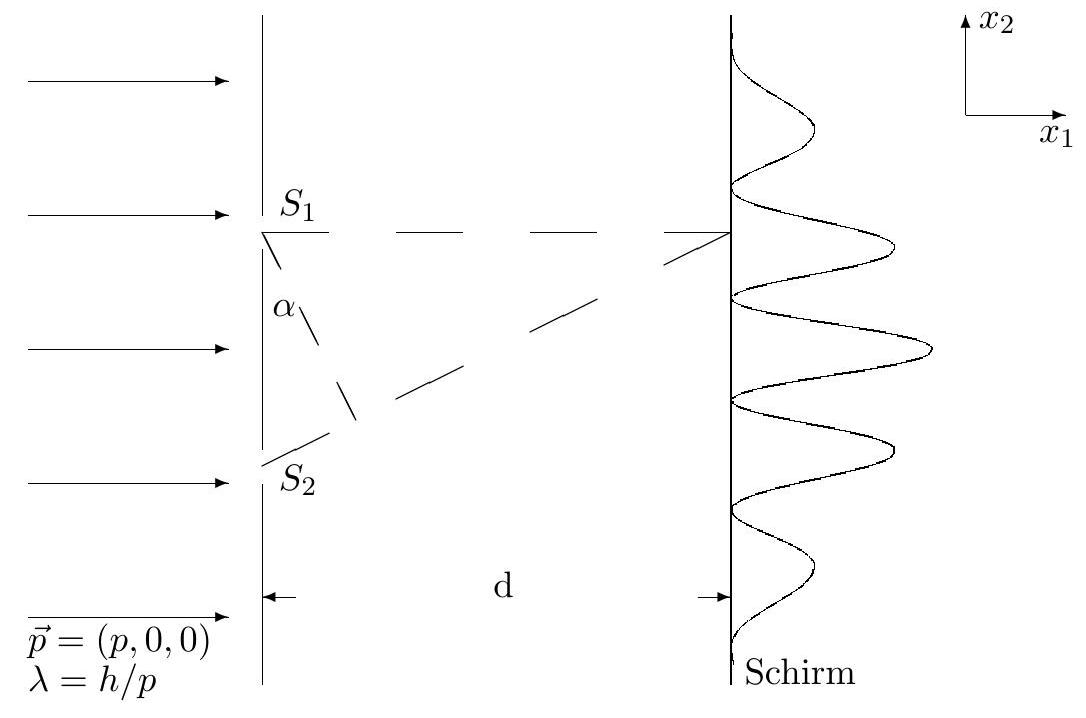
\includegraphics[scale=0.2, center]{2025_05_21_11b1754c718f6fcf84f8g-19}

Von links fällt eine ebene Welle mit Frequenz $\omega=\frac{E}{\hbar}=\frac{1}{\hbar}\left(\frac{1}{2 m} \vec{p}^{2}\right)$ und Wellenvektor $\vec{k}=\frac{1}{\hbar} \vec{p}$ auf eine Blende mit den Spalten $S_{1}$ und $S_{2}$, die sich im Abstand $a$ voneinander befinden. Die Spalten sind kohärente Quellen für die Kugelwellen ${ }^{9}$
$$
A_{1} \frac{e^{-i(\omega t-k|\vec{x}-\vec{a} / 2|)}}{|\vec{x}-\vec{a} / 2|}, \quad A_{2} \frac{e^{-i(\omega t-k|\vec{x}+\vec{a} / 2|)}}{|\vec{x}+\vec{a} / 2|}, \quad k=|\vec{k}|=\frac{2 \pi}{\lambda}
$$
die sich hinter der Blende überlagern:
$$
\psi(\vec{x}, t)=A_{1} \frac{e^{-i(\omega t-k|\vec{x}-\vec{a} / 2|)}}{|\vec{x}-\vec{a} / 2|}+A_{2} \frac{e^{-i(\omega t-k|\vec{x}+\vec{a} / 2|)}}{|\vec{x}+\vec{a} / 2|}
$$
Die zugehörige Intensität (unnormierte Wahrscheinlichkeitsdichte) ist
$$
|\psi(\vec{x}, t)|^{2}=\frac{\left|A_{1}\right|^{2}}{(\vec{x}-\vec{a} / 2)^{2}}+\frac{\left|A_{2}\right|^{2}}{(\vec{x}+\vec{a} / 2)^{2}}+\Re e\left(\frac{2 A_{1} A_{2}^{*} e^{i k(|\vec{x}-\vec{a} / 2|-|\vec{x}+\vec{a} / 2|)}}{|\vec{x}-\vec{a} / 2||\vec{x}+\vec{a} / 2|}\right)
$$
Der letzte Term ist für die Interferenzen auf dem Schirm verantwortlich, welche als Funktion der Gangdiffernez $\Delta x=|\vec{x}-\vec{a} / 2|-|\vec{x}+\vec{a} / 2|$ auftreten. Letzter lässt sich via $\Delta x=a \sin \alpha$ durch den Winkel $\alpha$ (siehe Abbildung) ausdrücken.
\end{EXA}




\subsubsection*{Wellen-Bild}


\begin{REM}{QM-G25-11-02}{Inferenzmaxima des Doppelspaltexperiments}
Die Interferenz-Maxima treten beim Doppelspaltexeriment auf wenn die Gangdiffernz $\Delta x$ ein Vielfaches der Wellenlänge $\lambda=2 \pi / k$ ist, also wenn
$$
a \sin \alpha_{n}=n \lambda
$$
gilt. Die Abstände der Maxima betragen auf dem Schirm
$$
d \sin \alpha_{n+1}-d \sin \alpha_{n} \approx \frac{d \lambda}{a}
$$
Hält man einen Spalt zu, so verschwindet das zugehörige $A_{i}$ und ebenso das Interferenzbild.
\end{REM}


\subsubsection*{Ein-Teilchen Interferenz}


\begin{REM}{QM-G25-11-03}{Ein-Teilchen Inferenz}
Die Interferenz verschwindet nicht, wenn man die Intensität des einfallenden Elektronenstrahl so stark verringert, daß immer nur ein einziges Elektron gleichzeitig in der Apparatur ist. Für eine genügende Statistik ist die Messung dann natürlich viele Male zu wiederholen.
\end{REM}

Einzelne Elektronen interferieren mit sich selber. Dies ist für alle Materiewellen der Fall. Da Elementarteilchen vom selben Typus ununterscheidbar sind, ist diese Aussage für den Viel-Teilchen Fall zu spezifizieren.





\subsection*{Ehrenfest Theorem}


\subsubsection*{Hermitisch konjungierte Operatoren}

\begin{DEF}{QM-G25-05-07}{Hermetisch konjugierter Operator}
Mit $A^{\dagger}$ bezeichnet man den zu $A$ hermitisch konjungierten Operator. In Matrix Notation transponiert man die Matrix und nimmt dann die komplex-konjungierte Werte
$$
A \hat{=} A_{i j}, \quad\left(A^{\dagger}\right)_{i j}=A_{j i}^{*}
$$
Es folgt
$$
(A \psi)^{*}=\psi^{*} A^{\dagger}
$$
was sich in Matrix-Notation mit $\psi=\left(\psi_{1}, \psi_{2}, \ldots\right)$ einfach nachvollziehen lässt:
$$
(A \psi)_{i}=\sum_{k} A_{i k} \psi_{k}, \quad\left((A \psi)^{*}\right)_{i}=\sum_{k} A_{i k}^{*} \psi_{k}^{*}=\sum_{k}\left(A^{\dagger}\right)_{k i} \psi_{k}^{*}=\left(\psi^{*} A^{\dagger}\right)_{i}
$$
\end{DEF}


\begin{CONC}{QM-G25-01-02}{Hermetisch konjugierte Schrödinger-Gleichung}
Angewandt auf die Schrödinger-Gleichung folgt
$$
i \hbar \dot{\psi}=H \psi, \quad-i \hbar \dot{\psi}^{*}=\psi^{*} H^{\dagger}=\psi^{*} H
$$
letzteres da der Hamilton-Operator symmetrisch und reel is, und damit selbst-adjungiert, d.h. es gilt $H=H^{\dagger}$.
\end{CONC}



\subsubsection*{Bewegungsgleichung für Erwartungswerte}


\begin{CONC}{QM-G25-01-03}{Ehrenfest Theorem für die Bewegungsgleichung des Erwartungswertes}
Die zeitliche Entwicklung von eines Erwartungwerts $\langle A\rangle$ is durch
$$
i \hbar \frac{d}{d t}\langle A\rangle=i \hbar \frac{d}{d t} \int d^{3} x \psi^{*} A \psi=\int d^{3} x \psi^{*} A(H \psi)-\int d^{3} x\left(\psi^{*} H\right) A \psi
$$
gegeben. Für den ersten Term haben wir die Schrödinger Gleichung $i \hbar \dot{\psi}=H \psi$ verwendet, und im zweiten Term die komplex-konjungierte Schrödinger Gleichung $-i \hbar \dot{\psi}^{*}=\psi^{*} H$. Hier haben wir angenommen, dass der Operator $A$ selber nicht explizit von der Zeit abhängt. Sollte das der Fall sein, ergibt sich insgesamt
$$
i \hbar \frac{d}{d t}\langle A\rangle=\langle[A, H]\rangle+i \hbar\left\langle\frac{\partial A}{\partial t}\right\rangle
$$
was man als Ehrenfest Theorem bezeichnet. Den Kommutator $[A, H]=A H-H A$ hatten wir bereits eingeführt.
\end{CONC}



\subsubsection*{Quasiklassische Bewegung}



\begin{CONC}{QM-G25-01-04}{Quasiklassische von Teilchen in zeitunabhängigen Potentialen}
Wir wenden das Ehrenfest Theorem auf den Impuls- und den Orts-Operator an. Für ein Teilchen in einem Zeit-unabhängignen Potential $V(x)$ gilt
$$
H=\frac{p^{2}}{2 m}+V(x), \quad[p, H]=[p, V(x)], \quad[x, H]=\left[x, p^{2}\right] / 2 m
$$
da Operatoren mit sich selber vertauschen. Der erste Term ergibt
$$
[p, H]=\frac{\hbar}{i}\left(\nabla_{x} V(x)-V(x) \nabla_{x}\right)=\frac{\hbar}{i} V^{\prime}
$$
während wir den zweiten Term mit Hilfe von $[x, p]=i \hbar$ zu
$$
\left[x, p^{2}\right]=x p^{2}-p^{2} x=(x p-p x+p x) p-p^{2} x=i \hbar p+p[x, p]=2 i \hbar p
$$
umformen. In das Ehrenfest Theorem eingesetzt finden wir
$$
i \hbar \frac{d}{d t}\langle p\rangle=\frac{\hbar}{i}\left\langle V^{\prime}\right\rangle, \quad i \hbar \frac{d}{d t}\langle x\rangle=\frac{i \hbar}{m}\langle p\rangle
$$
was zusammen
$$
m \frac{d}{d t}\langle x\rangle=\langle p\rangle \quad \frac{d}{d t}\langle p\rangle=-\left\langle V^{\prime}\right\rangle
$$
ergibt. Die Erwartungswerte von Operatoren gehorchen also den klassischen Bewegungsgleichungen. Dieses ist allerding nicht verwunderlich, da die Schrödinger-Gleichung dem Korrespondenzprinzip genügt.
\end{CONC}














\pagebreak


\section{Eindimensionale Systeme}




\subsection{Stationäre Schrödinger-Gleichung}


\subsubsection*{Seperation der Variabeln}


\begin{CONC}{QM-G25-12-01}{Herleitung der stationären 1d Schrödinger-Gleichung für zeitunabhängige Potentiale}
Ist das Potential $V(\vec{x})$ von der Zeit $t$ unabhängig, so kann man für die zeitabhängige Schrödinger-Gleichung $i \hbar \dot{\psi}(\vec{x}, t)=H \psi(\vec{x}, t)$ nach Lösungen der Form
$$
\psi(\vec{x}, t)=\sigma(t) u(\vec{x})
$$
suchen (Separation der Variablen). Dies führt zu
$$
i \hbar u(\vec{x}) \frac{d}{d t} \sigma(t)=\left[-\frac{\hbar^{2}}{2 m_{e}} \Delta u(\vec{x})+V(\vec{x}) u(\vec{x})\right] \sigma(t)
$$
Dividiert man durch $\sigma(t) u(\vec{x}) \neq 0$, so erhält man
$$
i \hbar \frac{1}{\sigma(t)} \frac{d \sigma(t)}{d t}=\frac{1}{u(\vec{x})} \mathbf{H} u(\vec{x}), \quad \mathbf{H}=-\frac{\hbar^{2}}{2 m_{e}} \Delta+V(\vec{x})
$$
Da die linke Seite eine Funktion der unabhängigen Variablen $t$, die rechte Seite eine Funktion der unabhängigen Variablen $\vec{x}$ ist, muß
$$
i \hbar \frac{1}{\sigma(t)} \frac{d \sigma(t)}{d t}=E=\mathrm{const}
$$
gelten, d.h.
$$
\sigma(t)=C e^{-i E t / \hbar}, \quad C=\text { const. }
$$
und
$$
\mathbf{H} u(\vec{x})=\left(-\frac{\hbar^{2}}{2 m_{e}} \Delta u(\vec{x})+V(\vec{x}) u(\vec{x})\right)=E u(\vec{x})
$$
Dies ist die zeitunabhängige oder stationäre Schrödinger-Gleichung. Die stationäre SchrödingerGleichung hat die Form einer Eigenwert-Gleichung.
\end{CONC}



\subsubsection*{Eigenwerte und Eigenfunktionen}


\begin{DEF}{QM-G25-12-02}{Eigenwerte von Matrizen}
Sei A eine $n \times n$ Matrix in einem $n$-dimensionalen Vektorraum, und $\vec{v}$ ein $n$ dimensionaler Vektor mit der Eigenschaft
$$
\mathbf{A} \vec{v}=a \vec{v}, \quad a \in \mathbb{R}
$$
so ist $a$ ein Eigenwert von $\mathbf{A}$ und $\vec{v}$ ein Eigenvektor von A zum Eigenwert $a: \vec{v}=\vec{v}_{a}$.
\end{DEF}

\begin{DEF}{QM-G25-12-03}{Eigenfunktionen des Schrödinger-Opeartors}
Analog ist mit
$$
u(\vec{x})=u_{E}(\vec{x}), \quad \mathbf{H} u_{E}(\vec{x})=E u_{E}(\vec{x})
$$
$u(\vec{x})$ eine Eigenfunktion des Schrödinger-Operators H, hier zum Eigenwert E.
\end{DEF}



\subsubsection*{Überlagerung zweier Lösungen}


\begin{CONC}{QM-G25-12-04}{Superpositionslösungen der (stationären) Schrödinger-Gleichung}
Seien $\psi_{j}(\vec{x}, t)=\sigma_{j}(t) u_{E_{j}}(\vec{x})$ zwei Lösungen der Schrödinger-Gleichung, mit
$$
\sigma_{j}(t)=C_{j} e^{-i E_{j} t / \hbar} \quad \text { und } \quad u_{E_{j}}(\vec{x}), \quad j=1,2,
$$
so ist auch jede linear Superposition von $\psi_{1}$ und $\psi_{2}$ eine Lösung. Das heisst, es gilt
$$
i \hbar \partial_{t} \psi(\vec{x}, t)=\mathbf{H} \psi(\vec{x}, t), \quad \psi(\vec{x}, t)=\alpha_{1} \psi_{1}(\vec{x}, t)+\alpha_{2} \psi_{2}(\vec{x}, t),
$$
mit konstanten $\alpha_{j}$.
\end{CONC}


\subsubsection*{Eigenwert-Spektren}


\begin{CONC}{QM-G25-12-05}{Eigenwert-Spektrum des Hamilton-Operators}
Die Eigenwerte des Hamilton-Operators können diskret oder kontinuierlich sein:
$$
\begin{aligned}
-\infty<E_{1}, \ldots, E_{\nu}, \ldots & \text { diskrete Eigenwerte, } \\
\{-\infty<E<\infty\} & \text { kontinuierlich verteilte Eigenwerte. }
\end{aligned}
$$
Wegen der Linearität der Schrödinger-Gleichung sind beliebige Überlagerungen
$$
\psi(\vec{x}, t)=\sum_{\nu=1}^{\infty} C_{\nu} e^{-i E_{\nu} t / \hbar} u_{E_{\nu}}(\vec{x})+\int d E C(E) e^{-i E t / \hbar} u_{E}(\vec{x})
$$
der orthonomierten Eigenfunktionen $u_{E_{\nu}}(\vec{x})$ und $u_{E}(\vec{x})$ wiederum Lösungen von $\mathbf{H}$, mit $C_{\nu} \in \mathcal{C}$ und $C(E) \in \mathcal{C}$ und der Bedingung für die Normierung der Wellefunktion,
$$
\sum_{\nu}\left|C_{\nu}\right|^{2}+\int d E|C(E)|^{2}=1
$$

Man beachte, dass die Energie unten beschränkt sein muss, da das System sonst nicht stabil ist: $E \geq B>-\infty$.
\end{CONC}



\subsection*{Eigenfunktionen des Impulsoperators}


\begin{EXA}{QM-G25-12-06}{Ebene Wellen als Eigenfunktionen des Impulsoperators}
Als Beispiel betrachten wir die Eigenfunktionen $e_{p}(x)$ des Impulsoperators $\mathbf{P}=\frac{\hbar}{i} \frac{d}{d x}$ zum reellen Eigenwert $p$ :
$$
\mathbf{P} e_{p}(x)=\frac{\hbar}{i} \frac{d}{d x} e_{p}(x)=p e_{p}(x)
$$
Die Eigenlösungen sind offenbar $e_{p}(x)=C e^{i p x / \hbar}$, mit $C=$ const., also ebene Wellen.
\end{EXA}



\subsubsection{Eindimensionale Potentialstufe}


\begin{DEF}{QM-G25-13-01}{Setting für eindimensionale Potentialstufe und stationäre Schrödinger-Gleichung}
Wir betrachten das eindimensionale Potential
$$
\begin{array}{rlll}
V(x)=0 & \text { für } & x<0 \\
V(x)=V_{0}>0 & \text { für } & x>0
\end{array}
$$
Die zugehörige zeitunabhängige Schrödinger-Gleichung zum Eigenwerte $E$ lautet
$$
-\frac{\hbar^{2}}{2 m} \frac{d^{2} u(x)}{d x^{2}}+V(x) u(x)=E u(x)
$$
\end{DEF}


\subsubsection*{Stetigkeits-Bedingungen am Potentialsprung}


\begin{CONC}{QM-G25-13-02}{Stetigkeitsbedingungen am Potentialsprung}
Das Potential springt bei $x=0$ um $V_{0}$. Dahe stellt sich die Frage, ob die Wellenfunktion auch Diskontinuitäten aufweist. Aus
$$
\frac{d^{2} u(x)}{d x^{2}}=-\frac{2 m}{\hbar^{2}}(E-V) u(x)
$$
folgt, daß bei stetigem $u(x)$ die zweite Ableitung von $u$ (linke Seite) bei $x=0$ einen endlichen Sprung um $2 m V_{0} / \hbar^{2} u(0)$ macht.
Die erste Ableitung $d u / d x$ ist dagegen stetig:
$$
\begin{aligned}
\lim _{\epsilon \rightarrow 0}\left(\left.\frac{d u}{d x}\right|_{\epsilon}-\left.\frac{d u}{d x}\right|_{-\epsilon}\right) & =\lim _{\epsilon \rightarrow 0} \int_{-\epsilon}^{+\epsilon} d x \frac{d}{d x}\left(\frac{d u}{d x}\right) \\
& =\lim _{\epsilon \rightarrow 0}-\frac{2 m}{\hbar^{2}} \int_{-\epsilon}^{+\epsilon} d x(E-V) u(x)=0
\end{aligned}
$$
da der Integrand endlich ist und das Integrationsintervall gegen Null tendiert.

Die Anschlussbedingung für $x=0$ ist also: $u(x)$ und $u^{\prime}(x)$ sind stetig. Allgemein spricht man auch von Randbedingungen.
\end{CONC}



\subsubsection{Streuzustände}


\begin{CONC}{QM-G25-13-03}{Ebene Wellen lösen stationäre Schrödinger-Gleichung mit konstantem Potential}
Wenn das Potential konstant ist, $V=0$ oder $V=V_{0}$, wird die stationäre-Schrödinger Gleichung durch ebene Wellen gelöst:
$$
u(x)=e^{ \pm i k x}, \quad \frac{(\hbar k)^{2}}{2 m}=E-V
$$
modulo einer Normierungskontanten. Dabei enspricht $+k$ und $-k$ links-, bzw. rechtslaufenden Wellen.
\end{CONC}


\subsubsection*{Einlaufende und reflektierte Welle}


\begin{CONC}{QM-G25-13-04}{Einlaufende und reflektierte Welle für $E>V_0, x<0$}
Wir betrachten $E>V_{0}$, die Eigenenergie des Zustandes ist also größer als die Potentialstufe. Klassisch würde ein von links einfallendews Elektron daher einfach durchlaufen. Um festzustellen, ob dies auch quantenmechanisch der Fall ist, gehen wir von der allgemeinen Lösung aus. D.h. wir betrachten $x \leq 0$ und
$$
x \leq 0: \quad u(x)=e^{i k x}+R e^{-i k x}, \quad k=\frac{1}{\hbar} \sqrt{2 m E}>0
$$
also eine allgemeine Superposition von einlaufender und reflektierte Welle. Zur einlaufenden Welle $(+k)$ wird die rücklaufende Welle $(-k)$ mit Amplitude $R$ zugemischt. Der entsprechende Teilchenfluss (die Wahrscheinlichkeits-Stromdichte) ist
$$
s(x)=\frac{\hbar}{2 m i}\left(u^{*} \frac{d u}{d x}-u \frac{d u^{*}}{d x}\right), \quad s_{-}=\frac{\hbar k}{m}\left(1-|R|^{2}\right)
$$
da sich die Mischterme gegenseitig aufheben.
\begin{itemize}
  \item $e^{i k x}$ beschreibt eine von links einfallende Welle mit Fluss $\hbar k / m>0$
  \item $R e^{-i k x}$ beschreibt eine an der Stufe reflektierte Welle mit Fluss $-|R|^{2} \hbar k / m$.
\end{itemize}
Die Anschlussbedingung bei $x=0$ bestimmt dabei $R$.
\end{CONC}



\subsubsection*{Transmitierte Welle}

\begin{CONC}{QM-G25-13-05}{Transmitierte Welle für $E>V_0, x>0$}
Wir betrachten $E>V_{0}$, die Eigenenergie des Zustandes ist also größer als die Potentialstufe. Die Lösung für $x \geq 0$ lautet
$$
x \geq 0: \quad u(x)=T e^{i q x}, \quad q=\frac{1}{\hbar} \sqrt{2 m\left(E-V_{0}\right)}, \quad s_{+}=\frac{\hbar q}{m}|T|^{2}
$$
Die ebenfalls mögliche Lösung $e^{-i q x}$ lassen wir weg, da von rechts keine Welle einfallen soll. $s_{+}=\frac{\hbar q}{m}|T|^{2}$ ist der nach rechts durchlaufende Strom.
\end{CONC}





\begin{CONC}{QM-G25-13-06}{Wellenanteile für stationäre Schrödinger-Gleichung mit  für $E>V_0$}
\begin{center}
\renewcommand{\arraystretch}{1.3}
\begin{tabular}{|c|c|l|}
\hline
\textbf{Welle} & \textbf{Fluss $s$} & \textbf{Interpretation} \\
\hline
$e^{i k x}$ & $\frac{\hbar k}{m}$ & Einlaufende Welle (von links) \\
$R e^{-i k x}$ & $-|R|^{2} \frac{\hbar k}{m}$ & Reflektierte Welle; $R$: Reflexionskoeffizient \\
$T e^{i q x}$ & $|T|^{2} \frac{\hbar q}{m}$ & Transmitierte Welle; $T$: Transmissionskoeffizient \\
\hline
\end{tabular}
\end{center}
\end{CONC}




\subsubsection*{Stetigkeitsbedingungen}

\begin{CONC}{QM-G25-13-07}{Reflexions und Transmissionskoeffizienten mit Randbedingung für $E>V_0$ bestimmen}
$u(x) \text { ist bei } x=0 \text { nur dann stetig wenn }$
$$
1+R=T
$$
erfüllt is. Analog ist die Ableitung $d u / d x$ bei $x=0$ stetig falls
$$
i k(1-R)=i q T
$$
gilt. Zusammen folgt
$$
R=\frac{k-q}{k+q}, \quad T=\frac{2 k}{k+q}
$$
Damit sind $R$ und $T$ als Funktionen von $E$ und $V_{0}$ bekannt.
\end{CONC}




\subsubsection*{Teilchenstromerhaltung}


\begin{CONC}{QM-G25-13-08}{Teilchenstromerhaltung für $E>V_0$}
Man rechnet unmittelbar nach, dass
$$
\frac{\hbar k}{m}\left(1-|R|^{2}\right)=\frac{\hbar q}{m}|T|^{2}
$$
gilt. Damit is $s(x)$ ebenfalls bei $x=0$ stetig. Das war zu erwarten, da der Teilchenstrom aufgrund der Kontinuitätsgleichung erhalten ist.
\end{CONC}

\begin{CONC}{QM-G25-13-09}{Unterschied zwischen CM und QM bzgl Potentialstufen}
Im Gegensatz zur klassischen Mechanik, für die für $E>V_{0}$ kein Teilchen an der Potentialstufe reflektiert würde, wird in der Quantenmechanik ein endliche Bruchteil, $|R|^{2}$, des Elektrons reflektiert.
\end{CONC}





\subsubsection{Reflektierte Zustände}


\begin{CONC}{QM-G25-13-11}{Charakterisierung der allgemeine Lösung für stationäre Schrödingergleichung mit $E<V_0$}
Wir betrachten nun $E<V_{0}$. Für $x \leq 0$ ist die allgemeie Lösung durch
$$
x \leq 0: \quad u(x)=A_{1} \sin k x+B_{1} \cos k x, \quad k=\frac{1}{\hbar} \sqrt{2 m E}
$$
gegeben, für $x \geq 0$ analog durch
$$
x \geq 0: \quad u(x)=A_{2} e^{-\kappa x}+B_{2} e^{\kappa x}, \quad \kappa=\frac{1}{\hbar} \sqrt{2 m\left(V_{0}-E\right)}
$$

Aus physikalischen Gründen (Normierbarkeit) kann $u(x)$ für $x>0$ nicht beliebig groß werden, woraus $B_{2}=0$ folgt.
\end{CONC}


\subsubsection*{Stetigkeitsbedingungen}


\begin{CONC}{QM-G25-13-12}{Stetigkeitsbedingungen für stationäre Schrödinger-Gleichung für $E<V_0$}
Die Bedingung der Stetigkeit von $u(x)$ und von $d u / d x$ für $x=0$ ergibt
$$
A_{2}=B_{1}, \quad A_{1} k=-A_{2},
$$
woraus
$$
\begin{array}{ll}
x \leq 0: & u(x)=A_{1}\left(\sin k x-\frac{k}{\kappa} \cos k x\right) \\
x \geq 0: & u(x)=-A_{1} \frac{k}{\kappa} e^{-\kappa x}
\end{array}
$$
folgt.

\subsubsection*{Bemerkungen}
\begin{itemize}
  \item Es ist überall $s(x)=0$. Stehende Wellen transportieren keine Teilchen.
  \item Im Gegensatz zum klassischen Fall dringt ein Bruchteil der Teilchen auch in das "verbotene" Gebiet $x>0$ ein. Im klassisch verbotenem Bereich fällt die Teilchendichte $|u(x)|^{2}$ exponentiell ab, mit der Eindringstiefe
\end{itemize}

$$
\lambda=\frac{1}{2 \kappa}=\frac{\hbar / 2}{\sqrt{2 m\left(V_{0}-E\right)}}
$$
\end{CONC}

Diese Phänomene werden an allen Grenzflächen beobachtet, sie sind u.A. in der Halbleiterphysik von Bedeutung.





\pagebreak


\subsection{Potentialbarriere}




\begin{DEF}{QM-G25-14-01}{Potentialbarriere}
\begin{center}
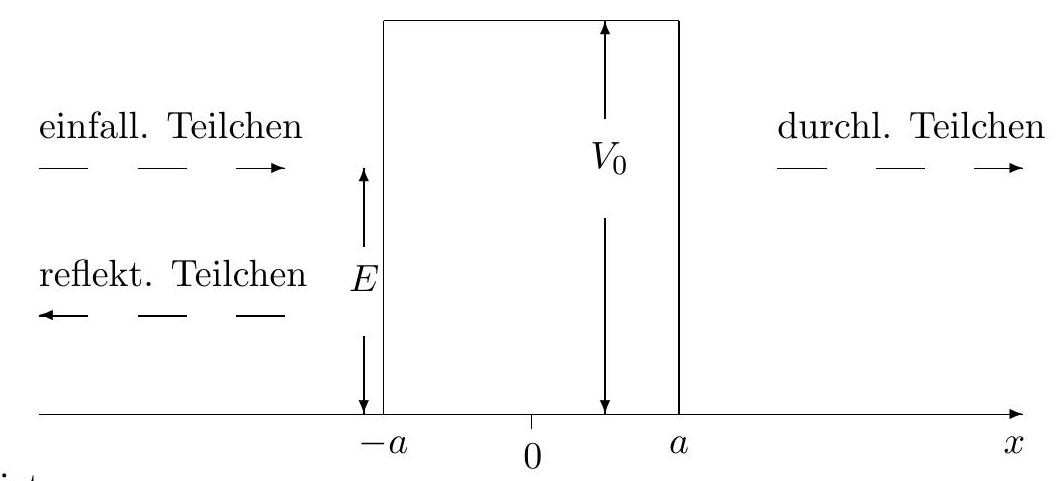
\includegraphics[scale=0.2]{2025_05_21_2790b5a0182e53887e3bg-08}
\end{center}

Das Potential ist:
$$
V(x)=\left\{\begin{array}{llc}
0 & \text { für } & x<-a \\
V_{0}>0 & \text { für } & -a<x<a \\
0 & \text { für } & x>a
\end{array}\right.
$$
\end{DEF}

\subsubsection*{Wellenfunktion}


\begin{CONC}{QM-G25-14-02}{Lösungsform für stationäre Schrödinger-Gleichung mit Potentialbarriere}
Wir nehmen an, dass von links Teilchen mit der Energie $E<V_{0}$ einfallen und zum Teil reflektiert werden. Von rechts sollen keine Teilchen einfallen. Wir haben somit
$$
\begin{aligned}
x<-a: & u(x) & =e^{i k x}+R e^{-i k x} & \\
-a<x<a: & u(x) & =A e^{-\kappa x}+B e^{\kappa x} & \\
x>a: & u(x) & =T e^{i k x} . &
\end{aligned}
$$
\end{CONC}


\subsubsection*{Stetigkeitsbedingungen}


\begin{CONC}{QM-G25-14-03}{Stetigkeitsbedingungen für stationäre Schrödinger-Gleichung mit Potentialbarriere}
Die Stetigkeit von $u(x)$ und $d u / d x$ bei $x= \pm a$ führt auf folgendes lineare Gleichungssystem, für die vier Grössen $R, A, B$ und $T$ :
$$
\begin{aligned}
& x=-a:\left\{\begin{aligned}
& e^{-i k a}+R e^{i k a}=A e^{\kappa a}+B e^{-\kappa a} \\
& i k\left(e^{-i k a}-R e^{i k a}\right)= \\
&\left.x=+a:-A e^{\kappa a}+B e^{-\kappa a}\right) \\
& A e^{-\kappa a}+B e^{\kappa a}=T e^{i k a} \\
& \kappa\left(-A e^{-\kappa a}+B e^{\kappa a}\right)=i k T e^{i k a}
\end{aligned}\right.
\end{aligned}
$$
Aus den beiden ersten Gleichungen ergibt sich
$$
\begin{aligned}
2 A e^{\kappa a} & =\left(1-i \frac{k}{\kappa}\right) e^{-i k a}+R\left(1+i \frac{k}{\kappa}\right) e^{i k a} \\
2 B e^{-\kappa a} & =\left(1+i \frac{k}{\kappa}\right) e^{-i k a}+R\left(1-i \frac{k}{\kappa}\right) e^{i k a}
\end{aligned}
$$
durch Addition und Subtraktion; ebenso aus den beiden letzten Gleichungen:
$$
\begin{aligned}
2 A e^{-\kappa a} & =\left(1-i \frac{k}{\kappa}\right) e^{i k a} T \\
2 B e^{\kappa a} & =\left(1+i \frac{k}{\kappa}\right) e^{i k a} T
\end{aligned}
$$
Die Quotienten führen zu
$$
\frac{A}{B}=\frac{\left(1-i \frac{k}{\kappa}\right) e^{-i k a}+R\left(1+i \frac{k}{\kappa}\right) e^{i k a}}{\left(1+i \frac{k}{\kappa}\right) e^{-i k a}+R\left(1-i \frac{k}{\kappa}\right) e^{i k a}} e^{-2 \kappa a}=\frac{\left(1-i \frac{k}{\kappa}\right) e^{i k a}}{\left(1+i \frac{k}{\kappa}\right) e^{i k a}} e^{2 \kappa a} .
$$
Mit $\rho=k / \kappa$ erhalten wir hieraus
$$
\left[\left(1+\rho^{2}\right) e^{-2 i k a}+R(1+i \rho)^{2}\right] e^{-2 \kappa a}=\left[\left(1+\rho^{2}\right) e^{-2 i k a}+R(1-i \rho)^{2}\right] e^{2 \kappa a}
$$
oder
$$
\left(1+\rho^{2}\right) e^{-2 i k a} \sinh (2 \kappa a)=R\left[\left(1+2 i \rho-\rho^{2}\right) e^{-2 \kappa a}-\left(1-2 i \rho-\rho^{2}\right) e^{2 \kappa a}\right]
$$
Setzen wir dies in den Quotienten aus den ersten beiden Gleichungen ein, so ergibt sich:
$$
R=e^{-2 i k a} \frac{\left(\kappa^{2}+k^{2}\right) \sinh (2 \kappa a)}{\left(k^{2}-\kappa^{2}\right) \sinh (2 \kappa a)+2 i \kappa k \cosh (2 a \kappa)}
$$
Analog findet man
$$
T=e^{-2 i k a} \frac{2 i \kappa k}{\left(k^{2}-\kappa^{2}\right) \sinh (2 \kappa a)+2 i \kappa k \cosh (2 a \kappa)}
$$
Daraus bekommt man folgende Absolutquadrate:
$$
\begin{aligned}
|R|^{2} & =\frac{\left(\kappa^{2}+k^{2}\right)^{2} \sinh ^{2}(2 \kappa a)}{\left(\kappa^{2}-k^{2}\right)^{2} \sinh ^{2}(2 \kappa a)+4 \kappa^{2} k^{2} \cosh ^{2}(2 \kappa a)} \\
|T|^{2} & =\frac{4 \kappa^{2} k^{2}}{\left(\kappa^{2}-k^{2}\right)^{2} \sinh ^{2}(2 \kappa a)+4 \kappa^{2} k^{2} \cosh ^{2}(2 \kappa a)}
\end{aligned}
$$
d.h. $|R|^{2}+|T|^{2}=1$, denn $\cosh ^{2}-\sinh ^{2}=1$.
\end{CONC}



\subsubsection*{Tunneleffekt}


\begin{CONC}{QM-G25-14-04}{Tunneleffekt für stationäre Schrödinger-Gleichung mit Potentialbarriere}
Obwohl $E<V_{0}$ können Teilchen durch die Barriere tunneln, wobei vor allem die Größe
$$
\kappa a=\frac{1}{\hbar} \sqrt{2 m a^{2}\left(V_{0}-E\right)}
$$
für den Bruchteil der durchlaufenden Elektronen verantwortlich ist.
\end{CONC}


\subsubsection*{Klassischer Grenzfall}


\begin{CONC}{QM-G25-14-05}{Klassischer Grenzfall des Tunneleffekt}
Wir betrachten nun den Fall kleiner Tunnelwahrscheinlichkeit, also z.B. $E \ll V_{0}$ oder allg.
$$
\kappa a \gg 1: \quad \sinh (2 \kappa a) \approx \frac{1}{2} e^{+2 \kappa a},
$$
d.h.
$$
|T|^{2} \approx \frac{(4 \kappa k)^{2}}{\left(\kappa^{2}+k^{2}\right)^{2}} e^{-4 \kappa a} \quad \kappa a=\frac{1}{\hbar} \sqrt{2 m a^{2}\left(V_{0}-E\right)}
$$
Wir bemerken, daß im klassischen Grenzfall $\hbar \rightarrow 0$ das Produkt $\kappa a$ divergiert, mit $\kappa a \rightarrow$ $\infty$, die Tunnelrate ist daher exponentiell unterdrückt.
\end{CONC}



\subsubsection*{Allgemeine Tunnelbarriere}


\begin{CONC}{QM-G25-14-06}{Exponentialabschätzung der Tunnelwahrscheinlichkeit}
Ein allgemeines Tunnelpotential $V(x)$ kann man näherungsweise im klassichen Grenzfall behandeln. Dafür berücksichtigt man in obiger Formel nur die Exponentialfunktion, womit die Transmissionskoeffizienten näherungsweise multiplikativ sind. Teilen wir die Barriere in kleine Abschnitte, $a=a_{1}+a_{2}+\ldots$, dann gilt für die zugehörigen Transmissionskoeffizienten

$$
\left|T_{a}\right|^{2} \approx\left|T_{a_{1}}\right|^{2} \cdot\left|T_{a_{2}}\right|^{2} \cdot \ldots
$$

(Multiplikationssatz der Wahrscheinlichkeiten).\\
Approximiert man einen kontinuierlichen Potentialberg $V(x)$ durch immer kleinere Stufen der Dicke $a_{i}$, so erhält man, abgesehen von einem Normierungsfaktor,

$$
|T| \approx e^{-2 \int d x \sqrt{\left(2 m / \hbar^{2}\right)(V(x)-E)}}
$$

Der Tunneleffekt ist ein wichtiges physikalischen Phänomen. Er ist z.B. für den Kernzerfall sowie für die kalte Emission von Elektronen aus einer Metalloberfläche (Kathode) verantwortlich.\\
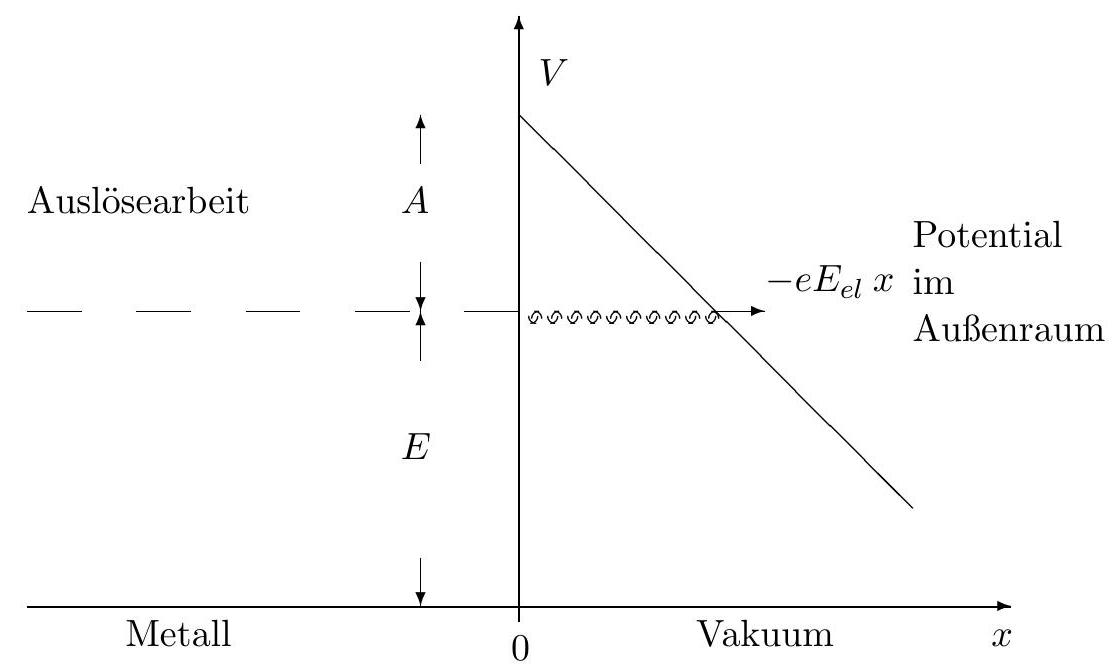
\includegraphics[scale=0.2, center]{2025_05_21_2790b5a0182e53887e3bg-11}
\end{CONC}






\pagebreak


\subsection*{Unendlich tiefer Potentialtopf}


\begin{CONC}{QM-G25-15-01}{Stationäre Schrödinger-Gleichung mit unendlichem Potentialtopf}
Wir studieren nun den Potentialverlauf
$$
\begin{array}{ll}
V(x)=0 & \text { für }-a<x<a \\
V(x)=\infty & \text { sonst }
\end{array}
$$
In Kap. 2.2 haben wir gesehen, daß die Wellenfunktion mit Energie $E<V_{0}$ in der Potentialstufe exponentiell unterdrückt wird. Für den unendlich tiefen Potentialtopf, mit $V_{0} \rightarrow \infty$, folgt also dass $u(x)=0$ für $|x| \geq a$ gilt. Im Topf selbst hat man
$$
\frac{d^{2} u}{d x^{2}}=-\frac{2 m E}{\hbar^{2}} u
$$
\end{CONC}

Keine Lösungen für $E<0$

\begin{CONC}{QM-G25-15-02}{Keine Lösung für stationäre Schrödinger-Gleichung mit unendlichem Potentialtopf und $E<0$}
Falls $E<0$ ist, so hat man für $-a<x<a$ die Lösungen
$$
u(x)=A_{1} e^{\kappa x}+A_{2} e^{-\kappa x}, \quad \kappa=\frac{1}{\hbar}(-2 m E)^{\frac{1}{2}}
$$
mit denen man die Randbedingungen $u(a)=u(-a)=0$ jedoch nur mit $A_{1}=A_{2}=0$ erfüllen kann. Es gibt also keine Lösungen für das Problem mit $E<0$.
\end{CONC}

\subsubsection*{Lösungen für $E>0$}

\begin{CONC}{QM-G25-15-03}{Lösung für stationäre Schrödinger-Gleichung mit unendlichem Potentialtopf und $E>0$}
Für $E>0$ gilt
$$
\frac{d^{2} u}{d x^{2}}=-k^{2} u(x), \quad k=\frac{1}{\hbar} \sqrt{2 m E}
$$
für $-a<x<a$, mit den Lösungen
$$
\begin{array}{ll}
u^{(-)}(x)=A^{(-)} \sin k x & (\text { ungerade Funktion in } x) \\
u^{(+)}(x)=A^{(+)} \cos k x & (\text { gerade Funktion in } x)
\end{array}
$$
\end{CONC}



\subsubsection*{Antisymmetrische Lösung}


\begin{CONC}{QM-G25-15-04}{Antisymmetrische Lösung für stationäre Schrödinger-Gleichung mit unendlichem Potentialtopf und $E>0$}
Aus der Randbedingung $\sin (a x)=0$ für die ungerade (antisymmetrische) Lösung folgt $k a=n \pi$, mit $n=1,2,3, \ldots$. Es sind also nur diskrete (bestimmte) Werte von $k$ (und damit der Energie E) mit der Randbedingung vertäglich. Die Eigenwerte sind somit quantisiert.

Die zulässigen Energiewerte sind
$$
E_{n}^{(-)}=\frac{n^{2} \pi^{2} \hbar^{2}}{2 m a^{2}}, \quad n=1,2,3, \ldots
$$
Die Normierung der zugehörigen Eigenfunktionen
$$
u_{n}^{(-)}=A^{(-)} \sin \left(\frac{n \pi x}{a}\right)
$$
gemäß $\int_{-a}^{a} u^{*}(x) u(x) d x=1$ ergibt $A^{(-)}=(a)^{-\frac{1}{2}}$, also
$$
u_{n}^{(-)}(x)=a^{-\frac{1}{2}} \sin \left(\frac{n \pi x}{a}\right), \quad n=1,2,3, \ldots
$$
\end{CONC}

\subsubsection*{Symmetrische Lösung}

\begin{CONC}{QM-G25-15-05}{Symmetrische Lösung für stationäre Schrödinger-Gleichung mit unendlichem Potentialtopf und $E>0$}
Für die gerade (symmetrische) Lösung folgt aus $\cos k a=0$, dass hier $k a=(n+1 / 2) \pi$ gilt, wobei $n$ eine ganze Zahl ist. Damit lauten die Eigenwerte
$$
E_{n}^{(+)}=\frac{(n+1 / 2)^{2} \pi^{2} \hbar^{2}}{2 m a^{2}}, \quad n=0,1,2, \ldots
$$
Die zugehörigen (normierten) Eigenfunktionen sind
$$
u_{n}^{(+)}=a^{-\frac{1}{2}} \cos \left[(n+1 / 2) \frac{\pi x}{a}\right], \quad n=0,1,2, \cdots
$$
\end{CONC}


\subsubsection*{Grundzustandsenergie}


\begin{CONC}{QM-G25-15-06}{Grundzustandenergie für Lösungen der stationäre Schrödinger-Gleichung mit unendlichem Potentialtopf und $E>0$}
Der tiefstmögliche Energiewert - die Grundzustandsenergie - ist
$$
E_{n=0}^{(+)}=\frac{\pi^{2} \hbar^{2}}{8 m a^{2}}
$$
Der niedrigste antisymmetriche Zustand, $u_{n=1}^{(-)}(x)$, hat die eine höhre Energie, $E_{n=1}^{(-)}=$ $4 E_{n=0}^{(+)}$.
\end{CONC}


\subsubsection*{Knoten der Wellenfunktion}

\begin{CONC}{QM-G25-15-07}{Knoten der Wellenfunktion}
Die Energien $E_{n}^{( \pm)}$sind jeweils um so größer, je größer die Zahl der Nullstellen (Knoten) der zugehörigen Eigenfunktionen $u_{n}^{( \pm)}(x)$ im Intervall $[-a,+a]$ ist. Je mehr Knoten, desto schneller verändert sich die Wellefunktion, desto grösser der Gradient, desto grösser damit auch die kinetische Energie.

Die Wellenfunktion $u_{n=0}^{(+)}=a^{-1 / 2} \cos \pi x /(2 a)$ des Grundzustandes hat keine Nullstelle für $|x|<a$.
\end{CONC}



\subsubsection*{Orthogonalität}

\begin{CONC}{QM-G25-15-08}{Orthogonalität von Lösungen der stationäre Schrödinger-Gleichung mit unendlichem Potentialtopf und $E>0$}
Mittels der Beziehungen
$$
\begin{aligned}
2 \cos \alpha_{1} \cos \alpha_{2} & =\cos \left(\alpha_{1}+\alpha_{2}\right)+\cos \left(\alpha_{1}-\alpha_{2}\right) \\
2 \sin \alpha_{1} \sin \alpha_{2} & =\cos \left(\alpha_{1}-\alpha_{2}\right)-\cos \left(\alpha_{1}+\alpha_{2}\right) \\
2 \sin \alpha_{1} \cos \alpha_{2} & =\sin \left(\alpha_{1}+\alpha_{2}\right)+\sin \left(\alpha_{1}-\alpha_{2}\right)
\end{aligned}
$$
erhält man mit $\sigma= \pm$ die Orthogonalitätsbeziehungen
$$
\int_{-a}^{a} d x\left(u_{m}^{(\sigma)}\right)^{*}(x) u_{n}^{(\sigma)}(x)=\delta_{m n}, \quad \int_{-a}^{a} d x\left(u_{m}^{(+)}\right)^{*}(x) u_{n}^{(-)}(x)=0
$$
Eigenfunktionen zu verschiedenen Eigenwerten $E_{n}^{( \pm)}$sind bezügliche des Skalarproduktes
$$
(\psi, \phi)=\int d x \psi^{*}(x) \phi(x)
$$
zueinander orthogonal:
$$
\left(u_{n}^{(\gamma)}, u_{m}^{(\alpha)}\right)=\delta_{n, m} \delta_{\gamma, \delta}, \quad \gamma, \alpha= \pm
$$
Das war zu erwarten, da der Hamilton-Operator symmetrisch ist, und symmetrische Matrizen otrhogonale Eigenfunktionen haben. Mehr dazu später.
\end{CONC}


\subsubsection*{1. Erwartungswerte}


\begin{CONC}{QM-G25-15-09}{Verschwinden der Erwartungswerte $\langle x \rangle$, $\langle p \rangle$}
Aufgrund der Paritätsstruktur der Eigenfunktionen gilt:
\[
\langle x \rangle = \langle p \rangle = 0
\]
Beispielhaft:
\[
\langle x \rangle = \int_{-a}^{a} \sin^2\left(\frac{n \pi x}{a}\right) x\, dx = 0
\]
wegen Antisymmetrie des Integranden.
\end{CONC}


\subsubsection*{2. Erwartungswerte von $x^2$ und $p^2$}


\begin{CONC}{QM-G25-15-10}{Erwartungswert von $p^2$ (Impulsquadrat)}
Da $\hat{H} = \frac{\hat{p}^2}{2m}$ und $E_n = \langle \hat{H} \rangle$, folgt:
\[
\langle p^2 \rangle_n^{(\pm)} = 2m E_n^{(\pm)} = \int_{-a}^{a} u_n^{(\pm)}(x) \left(-\hbar^2 \frac{d^2}{dx^2} \right) u_n^{(\pm)}(x)\, dx
\]
\end{CONC}



\begin{CONC}{QM-G25-15-11}{Erwartungswert von $x^2$ (Ortsquadrat)}
Für ungerade Eigenfunktionen:
\[
\langle x^2 \rangle_n^{(-)} = \frac{a^2}{3} \left(1 - \frac{3}{2\pi^2 n^2} \right)
\]
Dies folgt über die Substitution $y = \frac{\pi x}{a}$ und partielle Integration.
\end{CONC}


\subsubsection*{3. Unschärfen $\Delta x$ und $\Delta p$}

\begin{CONC}{QM-G25-15-13}{Unschärfen $\Delta x$ und $\Delta p$}
Da $\langle x \rangle = \langle p \rangle = 0$, sind die Unschärfen einfach:
\[
(\Delta x)^2 = \langle x^2 \rangle, \quad (\Delta p)^2 = \langle p^2 \rangle
\]
Die daraus folgenden Resultate lauten:

- Für ungerade Zustände \( u_n^{(-)} \):
  \[
  \Delta p_n^{(-)} = \frac{n \pi \hbar}{a}, \quad
  \Delta x_n^{(-)} = \frac{a}{\sqrt{3}} \left(1 - \frac{3}{2\pi^2 n^2} \right)^{1/2}
  \]

- Für gerade Zustände \( u_n^{(+)} \):
  \[
  \Delta p_n^{(+)} = \left(n + \frac{1}{2} \right) \frac{\pi \hbar}{a}, \quad
  \Delta x_n^{(+)} = \frac{a}{\sqrt{3}} \left(1 - \frac{3}{2\pi^2 (n + \frac{1}{2})^2} \right)^{1/2}
  \]
\end{CONC}

\subsubsection*{4. Produkt der Unschärfen: Heisenbergsche Unschärferelation}

\begin{CONC}{QM-G25-15-14}{Heisenberg Unschärferelation für stationäre Schrödinger-Gleichung mit unendlichem Potentialtopf und $E>0$}
Die Produkte der Unschärfen ergeben:
\[
\begin{aligned}
\Delta x_n^{(-)} \cdot \Delta p_n^{(-)} &= \frac{\hbar}{\sqrt{3}} \left(n^2 \pi^2 - \frac{3}{2} \right)^{1/2} \\
\Delta x_n^{(+)} \cdot \Delta p_n^{(+)} &= \frac{\hbar}{\sqrt{3}} \left((n + \tfrac{1}{2})^2 \pi^2 - \frac{3}{2} \right)^{1/2}
\end{aligned}
\]
\end{CONC}

\subsubsection*{5. Minimale Unschärfe im Grundzustand}

\begin{CONC}{QM-G25-15-15}{Minimale Unschärfe im Grundzustand für stationäre Schrödinger-Gleichung mit unendlichem Potentialtopf und $E>0$}
Für den Grundzustand \( u_0^{(+)} \) ergibt sich:
\[
\Delta x \cdot \Delta p = \frac{\hbar}{\sqrt{3}} \left( \frac{\pi^2}{4} - \frac{3}{2} \right)^{1/2}
= 0.568\, \hbar > \frac{\hbar}{2}
\]

Damit ist die **Heisenbergsche Unschärferelation**
\[
\Delta x \cdot \Delta p \geq \frac{\hbar}{2}
\]
erfüllt, aber **nicht saturiert**, da die Zustände keine Gaussfunktionen sind.
\end{CONC}







\pagebreak


\subsection{Potentialtopf mit endlicher Tiefe}




\textbf{Potentialdefinition und allgemeine Lösung}



\begin{CONC}{QM-G25-16-02}{Potentialdefinition mit endlicher Tiefe und allgemeine Lösung}
Wir betrachten das Potential
\[
V(x) = \begin{cases}
    -V_0 & \text{für } |x| < a \\
    0    & \text{für } |x| > a
\end{cases}
\quad \text{mit } V_0 > 0
\]
Die Lösungen der stationären Schrödinger-Gleichung für gebundene Zustände ($E<0$) ergeben sich in drei Bereichen:
\[
\begin{array}{rll}
x < -a       & : & u(x) = B_- e^{\kappa x} \\
|x| < a      & : & u(x) = A_1 \cos(qx) + A_2 \sin(qx) \\
x > a        & : & u(x) = B_+ e^{-\kappa x}
\end{array}
\]
mit den Parametern:
\[
\kappa = \sqrt{\frac{-2mE}{\hbar^2}}, \quad q = \sqrt{\frac{2m(V_0 + E)}{\hbar^2}}
\]
\end{CONC}



\textbf{Stetigkeitsbedingungen an $x = \pm a$}

\begin{CONC}{QM-G25-16-03}{Stetigkeitsbedigungen für stationäre Schrödinger-Gleichung mit endlichem Potential}
Die Wellenfunktion und ihre Ableitung müssen stetig sein:
\[
\begin{aligned}
u(-a^-) &= u(-a^+), &\quad u'(-a^-) &= u'(-a^+) \\
u(+a^-) &= u(+a^+), &\quad u'(+a^-) &= u'(+a^+)
\end{aligned}
\]
Dies führt zu:
\[
\begin{aligned}
B_- e^{-\kappa a} &= A_1 \cos(qa) - A_2 \sin(qa) \\
\kappa B_- e^{-\kappa a} &= q (A_1 \sin(qa) + A_2 \cos(qa)) \\
B_+ e^{-\kappa a} &= A_1 \cos(qa) + A_2 \sin(qa) \\
\kappa B_+ e^{-\kappa a} &= q (A_1 \sin(qa) - A_2 \cos(qa))
\end{aligned}
\]
Kombination der Bedingungen ergibt:
\[
\kappa = q \cdot \frac{A_1 \sin(qa) \pm A_2 \cos(qa)}{A_1 \cos(qa) \mp A_2 \sin(qa)}
\Rightarrow \text{nur möglich für } A_1 = 0 \text{ oder } A_2 = 0
\]
\end{CONC}



\textbf{Parität und Symmetrie der Lösungen}

\begin{CONC}{QM-G25-16-04}{Parität des Schrödinger-Operators and Symmetrie von Lösungen}
Die Parität des Hamiltonoperators ($V(x) = V(-x)$) erlaubt nur vollständig symmetrische oder antisymmetrische Lösungen:
\begin{itemize}
\item Gerade Lösung (symmetrisch): \( u^{(+)}(x) = A \cos(qx) \)
\item Ungerade Lösung (antisymmetrisch): \( u^{(-)}(x) = A \sin(qx) \)
\end{itemize}
\end{CONC}



\textbf{Eigenwertbedingungen für gebundene Zustände}

\begin{CONC}{QM-G25-16-05}{Eigenwertbedingungen für gebundene Zustände von Schrödinger-Gleichung mit endlichem Potential}
Aus den Matching-Bedingungen ergeben sich die transzendenten Gleichungen:
\begin{itemize}
\item Gerade Zustände:
  \[
  \kappa = q \tan(qa)
  \]
\item Ungerade Zustände:
  \[
  \kappa = -q \cot(qa)
  \]
\end{itemize}
Einführung der dimensionslosen Variablen:
\[
b^2 = \frac{2m V_0 a^2}{\hbar^2}, \quad y = qa
\Rightarrow \kappa a = \sqrt{b^2 - y^2}
\]
Ergibt:
\begin{itemize}
\item Gerade:
  \[
  \sqrt{b^2 - (y^{(+)})^2} = y^{(+)} \tan y^{(+)}
  \]
\item Ungerade:
  \[
  \sqrt{b^2 - (y^{(-)})^2} = - y^{(-)} \cot y^{(-)}
  \]
\end{itemize}
\end{CONC}


\textbf{Existenzbedingungen für Zustände}

\begin{CONC}{QM-G25-16-06}{Existenzbedingungen für gebundene Zustände von Schrödinger-Gleichung mit endlichem Potential}
\begin{itemize}
\item Mindestens ein gebundener Zustand (symmetrisch) existiert immer:
  \[
  0 < y^{(+)} < \frac{\pi}{2}
  \]
\item Antisymmetrischer Zustand nur möglich, wenn:
  \[
  b^2 > \frac{\pi^2}{4}
  \quad \text{(d.h. Topf tief genug)}
  \]
\end{itemize}
\end{CONC}



\textbf{Grenzfall: Tiefer Potentialtopf $V_0 \rightarrow \infty$}


\begin{EXA}{QM-G25-16-07}{Tiefer Potentialtopf}
Für \( b^2 \gg y^2 \) folgt näherungsweise:
\[
y_n^{(+)} \approx \left(n + \frac{1}{2}\right)\pi, \quad
y_n^{(-)} \approx n \pi
\Rightarrow \text{Übergang zum unendlichen Potentialtopf}
\]
Diese Energien entsprechen dann:
\[
E_n^{(\pm)} = \frac{\hbar^2 (y_n^{(\pm)})^2}{2ma^2} - V_0
\]
\end{EXA}




\begin{REM}{QM-G25-16-08}{Charakteristika gebundener Zustände im endlichen Potentialtopf}
\begin{tabular}{|c|c|c|}
\hline
\textbf{Abschnitt} & \textbf{Eigenfunktionsform} & \textbf{Existenzbedingung} \\
\hline
Symmetrisch & $u^{(+)}(x) = \cos(qx)$ & Immer \\
\hline
Antisymmetrisch & $u^{(-)}(x) = \sin(qx)$ & Nur wenn $b^2 > \frac{\pi^2}{4}$ \\
\hline
Tiefer Topf & $V_0 \to \infty$ & Übergang zu Standard-Energien des unendlichen Kastens \\
\hline
\end{tabular}
\end{REM}








\pagebreak



\subsection{Paritätsoperator}



\begin{DEF}{QM-G25-17-01}{Paritätsoperator}
Der \emph{Paritätsoperator} $\boldsymbol{\Pi}$ ist definiert durch
\[
(\boldsymbol{\Pi} u)(x) := u(-x)
\]
Er reflektiert also eine Funktion $u(x)$ an der $x=0$-Achse.
\end{DEF}



\begin{PROP}{QM-G25-17-03}{Eigenfunktionen des Paritätsoperators}
Die Eigenfunktionen des Operators $\boldsymbol{\Pi}$ sind entweder gerade oder ungerade Funktionen:
\[
\begin{aligned}
\boldsymbol{\Pi} u^{(+)}(x) &= u^{(+)}(-x) = +u^{(+)}(x) \\
\boldsymbol{\Pi} u^{(-)}(x) &= u^{(-)}(-x) = -u^{(-)}(x)
\end{aligned}
\]
Die zugehörigen Eigenwerte $\lambda = \pm 1$ nennt man die \emph{Parität} der Funktion.
\end{PROP}



\begin{LEM}{QM-G25-17-04}{Spektrum des Paritätsoperators}
Da $\boldsymbol{\Pi}^2 = \mathrm{id}$, sind die einzigen möglichen Eigenwerte von $\boldsymbol{\Pi}$ gegeben durch:
\[
\lambda = \pm 1
\]
\end{LEM}

\begin{PROP}{QM-G25-17-05}{Zerlegung nach Parität}
Jede Funktion $u(x)$ lässt sich eindeutig in einen geraden und einen ungeraden Anteil zerlegen:
\[
u(x) = \frac{1}{2}(u(x) + u(-x)) + \frac{1}{2}(u(x) - u(-x)) =: u^{(+)}(x) + u^{(-)}(x)
\]
Dabei ist $u^{(+)}$ gerade und $u^{(-)}$ ungerade.
\end{PROP}



\begin{CONC}{QM-G25-17-06}{Symmetrie des Hamiltonoperators}
Der Hamiltonoperator des Potentialtopfs
\[
\mathbf{H} = -\frac{\hbar^2}{2m} \frac{d^2}{dx^2} + V(x), \quad \text{mit } V(x) = V(-x)
\]
ist invariant unter dem Paritätsoperator:
\[
[\mathbf{H}, \boldsymbol{\Pi}] = 0
\]
\end{CONC}

\begin{CONC}{QM-G25-17-07}{Konservierte Parität}
Aus der Vertauschungsrelation $[\mathbf{H}, \boldsymbol{\Pi}] = 0$ folgt, dass Parität eine Erhaltungsgröße ist. Ist $\Psi(x,t)$ eine Lösung der Schrödingergleichung,
\[
i \hbar \partial_t \Psi(x,t) = \mathbf{H} \Psi(x,t),
\]
so ist auch $\boldsymbol{\Pi} \Psi(x,t)$ eine Lösung.
\end{CONC}


\begin{CONC}{QM-G25-17-08}{Zeitentwicklung separierter Paritäten}
Mit Hilfe der Projektoren
\[
\Psi^{(+)}(x, t) = \frac{1}{2}(1 + \boldsymbol{\Pi}) \Psi(x,t), \quad \Psi^{(-)}(x, t) = \frac{1}{2}(1 - \boldsymbol{\Pi}) \Psi(x,t)
\]
gilt:
\begin{itemize}
\item $\Psi^{(+)}$ und $\Psi^{(-)}$ sind jeweils Lösungen der Schrödinger-Gleichung.
\item Die Zeitentwicklung mischt die beiden Anteile nicht.
\end{itemize}
\end{CONC}


\begin{CONC}{QM-G25-17-09}{Klassifikation stationärer Zustände}
Jede Eigenfunktion $u(x)$ des Hamiltonoperators kann nach ihrer Parität klassifiziert werden. Es gilt also stets:
\[
u(x) \in \operatorname{Eig}(\boldsymbol{\Pi}, +1) \quad \text{oder} \quad u(x) \in \operatorname{Eig}(\boldsymbol{\Pi}, -1)
\]
\end{CONC}



\begin{PROP}{QM-G25-17-10}{Wirkung des Paritätsoperators auf Observablen}
Für Orts- und Impulsoperator gilt:
\[
\boldsymbol{\Pi} \mathbf{Q} = -\mathbf{Q} \boldsymbol{\Pi}, \quad \boldsymbol{\Pi} \mathbf{P} = -\mathbf{P} \boldsymbol{\Pi}
\]
Insbesondere ändert sich das Vorzeichen von Ort und Impuls unter Anwendung von $\boldsymbol{\Pi}$.
\end{PROP}



\begin{PROP}{QM-G25-17-11}{Hermitizität des Paritätsoperators}
Der Paritätsoperator ist hermitesch:
\[
\boldsymbol{\Pi}^\dagger = \boldsymbol{\Pi}
\]
\end{PROP}


Beweis: 

\begin{PROOF}{QM-G25-17-12}{P: Hermitizität des Paritätsoperators}
Für beliebige $u_1, u_2$ gilt
\[
(u_1, \boldsymbol{\Pi} u_2) = \int_{-a}^{a} u_1^*(x) u_2(-x)\, dx
\]
Substitution $x \mapsto -x$ liefert:
\[
= \int_{-a}^{a} u_1^*(-x) u_2(x)\, dx = (\boldsymbol{\Pi} u_1, u_2) = (u_2, \boldsymbol{\Pi} u_1)^*
\qed
\]
\end{PROOF}






\pagebreak



\subsection{Zusammenfassung}


\begin{CONC}{QM-G25-12-07}{Zusammenfassung der Ergebnisse für Eindimensionale Schrödinger-Gleichung}
Die Betrachtung der Quantenmechanik eindimensionaler Systeme erscheint auf den ersten Blick etwas akademisch. Aus zwei Gründen ist dieses Kapitel jedoch sehr wichtig. Einerseits gibt es es gerade durch die moderne Halbleitertechnik physikalische System (Quantendrähte, Quantendots), welche sich eindimensional verhalten und durch die hier entwickelte Theorie in erster Näherung beschrieben werden. Zudem konnten wir anhand der eindimensionalen Systeme einiges von allg. Bedeutung lernen:

\begin{enumerate}
  \item Die Existenz und Physik von Streuzuständen (Potentialstufe und Potentialbarriere). Sie haben ein kontinuierliches Energiespektrum.
  \item Die Physik des Tunneleffekts (Potentialbarriere). Als Funktion des Tunnelpotentials ist die Tunnelrate i.a. exponentiell klein.
  \item Die Eigenschaften der Eigenzustände in einem Potential $V(x)$, welches für $|x| \rightarrow$ $\infty$ divergiert (unendlich tiefer Potentialtopf): Alle Eigenenergien sind diskret und durch die Randbedingungen bestimmt. Ein weiteres Beispiel hierzu werden wir später mit dem harmonischen Oszillator kennelernen.
  \item Die Existenz von gebundenen Zuständen für ein Potential $V(x)$, welches für $|x| \rightarrow$ $\infty$ endlich bleibt (endlich tiefer Potentialtopf). Die Randbedingungen bestimmen die erlaubten Quantenzahlen. Gebundene Zustände werden wir beim Wasserstoffatoms wiedersehen, die Lösung der Schrödinger-Gleichung erfordert im Falle des Wasserstoffatoms jedoch einen viel höheren mathematischen Aufwand.
  \item Am Beispiel des Paritätsoperators haben wir gesehen, daß sich die Lösungen eines Hamiltonoperators nach den Eigenwerten seiner Symmetrieelemente klassifizieren lassen. Von diesem Umstand werden wir bei der Betrachtung des Wasserstoffatoms umfassenden Gebrauch machen.
\end{enumerate}
\end{CONC}








\pagebreak




\section{Der harmonische Oszillator}


\textbf{CTyp: Concept – Hamiltonoperator des harmonischen Oszillators}

\begin{DEF}{QM-G25-18-01}{Hamiltonoperator des harmonischen Oszillators}
Der klassische harmonische Oszillator wird durch die Hamiltonfunktion
\[
E=\frac{1}{2m}p^2 + \frac{b}{2}x^2, \quad b > 0
\]
beschrieben. Nach dem Korrespondenzprinzip ergibt sich daraus der Hamiltonoperator der Quantenmechanik:
\[
\mathbf{H} = -\frac{\hbar^2}{2m}\frac{d^2}{dx^2} + \frac{b}{2}x^2
\]
Dieser beschreibt die zeitunabhängige Schrödinger-Gleichung
\[
\mathbf{H} u(x) = E u(x).
\]
\end{DEF}



\textbf{CTyp: Concept – Randbedingungen für gebundene Zustände im Oszillatorpotential}

\begin{CONC}{QM-G25-18-02}{Randbedingungen für gebundene Zustände im Oszillatorpotential}
Das Potential $\frac{b}{2}x^2$ wächst mit $|x|$ und erzwingt die Bedingung:
\[
\lim_{|x|\to\infty} u(x) = 0, \quad \text{und} \quad \int_{-\infty}^{\infty} |u(x)|^2 \, dx = 1.
\]
Nur diskrete Eigenwerte $E$ erfüllen diese Normalisierungsbedingung.
\end{CONC}



\textbf{CTyp: Concept – Reskalierte Form der Schrödinger-Gleichung}



\begin{CONC}{QM-G25-18-03}{Reskalierte Form der Schrödinger-Gleichung}
Durch Einführung der charakteristischen Oszillatorfrequenz
\[
\omega = \sqrt{\frac{b}{m}}, \quad \beta^2 = \frac{m\omega}{\hbar}, \quad \varepsilon = \frac{2E}{\hbar\omega}
\]
wird der Hamiltonoperator
\[
\mathbf{H} = -\frac{\hbar^2}{2m} \frac{d^2}{dx^2} + \frac{b}{2} x^2
\]
in die dimensionslose Form überführt:
\[
\frac{1}{\beta^2} \frac{d^2 u}{dx^2} = \left( \beta^2 x^2 - \varepsilon \right) u(x).
\]
Dies vereinfacht die Analyse der asymptotischen Struktur.
\end{CONC}


\textbf{CTyp: Example – Lösung für $\varepsilon = 1$ (Grundzustand)}

\begin{EXA}{QM-G25-18-04}{Lösung für $\varepsilon = 1$ (Grundzustand)}
Für große $x$ liefert die asymptotische Gleichung
\[
u''_\infty = \beta^4 x^2 u_\infty
\]
die Lösung
\[
u_\infty(x) = e^{-\frac{1}{2}\beta^2 x^2}.
\]
Diese ist exakt für $\varepsilon = 1$, d.h. $E_0 = \frac{1}{2}\hbar\omega$. Die normierte Lösung ist
\[
u_0(x) = \left(\frac{\beta^2}{\pi}\right)^{1/4} e^{-\beta^2 x^2 / 2}.
\]
\end{EXA}



\textbf{CTyp: Definition – Erzeugungs- und Vernichtungsoperatoren im Oszillator}

\begin{DEF}{QM-G25-18-05}{Erzeugungs- und Vernichtungsoperatoren im Oszillator}
Definiert sind:
\[
\mathbf{a} = \frac{1}{\sqrt{2}} \left( \beta x + \frac{1}{\beta} \frac{d}{dx} \right), \quad
\mathbf{a}^+ = \frac{1}{\sqrt{2}} \left( \beta x - \frac{1}{\beta} \frac{d}{dx} \right).
\]
Diese Operatoren erfüllen:
\[
[\mathbf{a}, \mathbf{a}^+] = 1, \quad \mathbf{H} = \hbar\omega\left( \mathbf{a}^+ \mathbf{a} + \frac{1}{2} \right).
\]
\end{DEF}


\textbf{CTyp: Proposition – Charakterisierung des Grundzustands durch Vernichtungsoperator}

\begin{PROP}{QM-G25-18-06}{Charakterisierung des Grundzustands durch Vernichtungsoperator}
Der niedrigste Energiezustand $u_0(x)$ des harmonischen Oszillators erfüllt
\[
\mathbf{a} u_0 = 0.
\]
Dies führt auf die Differentialgleichung
\[
\frac{du}{dx} = -\beta^2 x u(x),
\]
deren Lösung
\[
u(x) = u_0(x) = \left(\frac{\beta^2}{\pi}\right)^{1/4} e^{-\frac{1}{2} \beta^2 x^2}
\]
genau dem zuvor gefundenen Grundzustand entspricht. Damit ist $\varepsilon = 1$, also $E_0 = \frac{1}{2} \hbar \omega$.
\end{PROP}


\textbf{CTyp: Concept – Wirkung der Leiteroperatoren auf Eigenzustände}

\begin{CONC}{QM-G25-18-07}{Wirkung der Leiteroperatoren auf Eigenzustände}
Für den Hamiltonoperator $\mathbf{H} = \hbar\omega(\mathbf{a}^+ \mathbf{a} + \frac{1}{2})$ gilt:
\[
\mathbf{H}(\mathbf{a} u) = \hbar\omega \left( \frac{\varepsilon}{2} - 1 \right) (\mathbf{a} u), \quad
\mathbf{H}(\mathbf{a}^+ u) = \hbar\omega \left( \frac{\varepsilon}{2} + 1 \right) (\mathbf{a}^+ u).
\]
Durch Iteration erreicht man stets den Grundzustand $u_0$.
\end{CONC}



\textbf{CTyp: Concept – Energiespektrum des harmonischen Oszillators}

\begin{CONC}{QM-G25-18-08}{Energiespektrum des harmonischen Oszillators}
Nur Werte $\varepsilon_n = 2n + 1$ sind erlaubt. Mit
\[
E = \frac{\hbar\omega}{2} \varepsilon \quad \Rightarrow \quad
E_n = \left( n + \frac{1}{2} \right) \hbar \omega, \quad n \in \mathbb{N}_0
\]
ergibt sich ein gleichabständiges, diskretes Energiespektrum.
\end{CONC}


\textbf{CTyp: Definition – Iterative Konstruktion der Eigenfunktionen}

\begin{DEF}{QM-G25-18-09}{Iterative Konstruktion der Eigenfunktionen}
Die normierten Eigenfunktionen $u_n(x)$ entstehen durch wiederholte Anwendung des Erzeugungsoperators:
\[
u_n(x) = \frac{1}{\sqrt{n!}} (\mathbf{a}^+)^n u_0(x), \quad u_0(x) = \left( \frac{\beta^2}{\pi} \right)^{1/4} e^{-\beta^2 x^2/2}.
\]
\end{DEF}



\textbf{CTyp: Concept – Orthonormalität und Vollständigkeit der Eigenfunktionen}

\begin{CONC}{QM-G25-18-10}{Orthonormalität und Vollständigkeit der Eigenfunktionen}
Verschiedene Eigenfunktionen $u_n$ des Operators $\mathbf{H}$ sind orthogonal:
\[
E_n \neq E_m \Rightarrow (u_n, u_m) = 0.
\]
Die Menge $\{u_n\}$ bildet eine vollständige orthonormale Basis des Hilbertraums.
\end{CONC}



\textbf{CTyp: Concept – Explizite Form der Eigenfunktionen mit Hermite-Polynomen}

\begin{CONC}{QM-G25-18-11}{Explizite Form der Eigenfunktionen mit Hermite-Polynomen}
Die Eigenfunktionen lassen sich durch Hermite-Polynome ausdrücken:
\[
u_n(x) = \sqrt{\beta} \left( \frac{1}{2^n n! \sqrt{\pi}} \right)^{1/2} e^{-\frac{1}{2} \beta^2 x^2} H_n(\beta x).
\]
Die $H_n(y)$ erfüllen:
\[
H_n''(y) - 2y H_n'(y) + 2n H_n(y) = 0.
\]
\end{CONC}


\textbf{CTyp: Concept – Matrixelemente der Oszillator-Operatoren}

\begin{CONC}{QM-G25-18-12}{Matrixelemente der Oszillator-Operatoren}
Die Operatoren $\mathbf{a}, \mathbf{a}^+$ haben Matrixelemente in der Basis $\{u_n\}$:
\[
\begin{aligned}
(u_m, \mathbf{a} u_n) &= \sqrt{n} \delta_{m,n-1} \\
(u_m, \mathbf{a}^+ u_n) &= \sqrt{n+1} \delta_{m,n+1}.
\end{aligned}
\]
Ferner:
\[
\begin{aligned}
(u_m, \mathbf{Q} u_n) &= \frac{1}{\sqrt{2}\beta} \left( \sqrt{n} \delta_{m,n-1} + \sqrt{n+1} \delta_{m,n+1} \right) \\
(u_m, \mathbf{P} u_n) &= \frac{\hbar\beta}{i\sqrt{2}} \left( \sqrt{n} \delta_{m,n-1} - \sqrt{n+1} \delta_{m,n+1} \right).
\end{aligned}
\]
\end{CONC}



\textbf{CTyp: Definition – Adjungierter Operator im Hilbertraum}

\begin{DEF}{QM-G25-05-08}{Adjungierter Operator im Hilbertraum}
Ein Operator $A$ besitzt einen Adjungierten $A^+$, falls gilt:
\[
(u, A \varphi) = (A^+ u, \varphi) \quad \text{für alle } \varphi \text{ im Definitionsbereich}.
\]
In Matrixnotation:
\[
(A^+)_{\mu\nu} = (A \varphi_\mu, \varphi_\nu)^* = A^*_{\nu\mu}.
\]
\end{DEF}


\textbf{CTyp: Definition – Selbstadjungierter Operator}

\begin{DEF}{QM-G25-05-09}{Selbstadjungierter Operator}
Ein Operator $A$ heißt selbstadjungiert, wenn
\[
(\varphi_\nu, A \varphi_\mu) = (A \varphi_\nu, \varphi_\mu),
\]
d.h. $A = A^+$. Selbstadjungierte Operatoren besitzen reelle Eigenwerte und hermitesche Matrixdarstellungen.
\end{DEF}


\textbf{CTyp: Concept – Physikalische Bedeutung selbstadjungierter Operatoren}

\begin{CONC}{QM-G25-05-10}{Physikalische Bedeutung selbstadjungierter Operatoren}
In der Quantenmechanik entsprechen alle Observablen selbstadjungierten Operatoren, insbesondere:
- Hamilton-Operator $\mathbf{H}$

- Ortsoperator $\mathbf{x}$

- Impulsoperator $\mathbf{p}$

Dies garantiert reale Messwerte.
\end{CONC}


\textbf{CTyp: Definition – Unitärer Operator}

\begin{DEF}{QM-G25-05-11}{Unitärer Operator}
Ein Operator $U$ heißt unitär, wenn
\[
U^+ = U^{-1}, \quad \Rightarrow \quad U^+ U = UU^+ = \mathbb{I}.
\]
Unitäre Operatoren erhalten das Skalarprodukt:
\[
(U u_1, U u_2) = (u_1, u_2).
\]
Beispiele: Orthogonale Transformationen, Zeitentwicklungsoperator.
\end{DEF}



\textbf{CTyp: Concept – Motivation für kohärente Zustände}

\begin{CONC}{QM-G25-18-17}{Motivation für kohärente Zustände}
Für alle Eigenzustände $u_n$ des harmonischen Oszillators gilt:
\[
(u_n, \mathbf{Q} u_n) = (u_n, \mathbf{P} u_n) = 0.
\]
Die klassische Bewegung $x(t) = A\sin(\omega t + \alpha)$ wird daher durch Erwartungswerte der Energieeigenzustände nicht wiedergegeben. Dies motiviert kohärente Überlagerungen.
\end{CONC}


\textbf{CTyp: Definition – Kohärente Zustände als Eigenfunktionen von $\mathbf{a}$}

\begin{DEF}{QM-G25-18-18}{Kohärente Zustände als Eigenfunktionen von $\mathbf{a}$}
Ein kohärenter Zustand $u_z(x)$ ist eine Eigenfunktion des Vernichtungsoperators:
\[
\mathbf{a} u_z(x) = z u_z(x), \quad z \in \mathbb{C}.
\]
\end{DEF}


\textbf{CTyp: Concept – Erwartungswerte im kohärenten Zustand}

\begin{CONC}{QM-G25-18-19}{Erwartungswerte im kohärenten Zustand}
Die Erwartungswerte lauten:
\[
\left(u_z, \mathbf{Q} u_z\right) = \frac{1}{\sqrt{2} \beta} (z + z^*), \quad
\left(u_z, \mathbf{P} u_z\right) = \frac{\hbar \beta}{i \sqrt{2}} (z - z^*).
\]
Diese sind im Allgemeinen nicht null.
\end{CONC}


\textbf{CTyp: Proposition – Darstellung kohärenter Zustände über $e^{z\mathbf{a}^+}$}

\begin{PROP}{QM-G25-18-21}{Darstellung kohärenter Zustände über $e^{z\mathbf{a}^+}$}
Sei $u_z(x)$ ein kohärenter Zustand mit $\mathbf{a} u_z = z u_z$. Die Eigenfunktion kann durch Entwicklung nach den Eigenzuständen $u_n$ des Oszillators dargestellt werden:
\[
u_z(x) = \sum_{n=0}^\infty (u_n, u_z) \, u_n(x),
\]
mit
\[
(u_n, u_z) = \frac{z^n}{\sqrt{n!}} (u_0, u_z).
\]
Daher folgt:
\[
u_z(x) = (u_0, u_z) \sum_{n=0}^\infty \frac{(z \mathbf{a}^+)^n}{n!} u_0(x) = (u_0, u_z) e^{z \mathbf{a}^+} u_0(x).
\]
\end{PROP}



\textbf{CTyp: Concept – Übervollständigkeit kohärenter Zustände}

\begin{CONC}{QM-G25-18-22}{Übervollständigkeit kohärenter Zustände}
Kohärente Zustände $u_z$ sind nicht orthogonal:
\[
(u_{z_2}, u_{z_1}) = \exp\left(-\tfrac{1}{2}|z_1|^2 - \tfrac{1}{2}|z_2|^2 + z_2^* z_1\right),
\]
bilden aber ein übervollständiges System.
\end{CONC}


\textbf{CTyp: Example – Ortsraumdarstellung kohärenter Zustände}

\begin{EXA}{QM-G25-18-23}{Ortsraumdarstellung kohärenter Zustände}
Die explizite Darstellung im Ortsraum lautet:
\[
u_z(x) = \left( \frac{\beta^2}{\pi} \right)^{1/4} \exp\left( -\tfrac{1}{2} \beta^2 x^2 + \sqrt{2} z \beta x - \tfrac{1}{2}|z|^2 - \tfrac{1}{2}z^2 \right).
\]
Dies ist ein gaußsches Wellenpaket.
\end{EXA}


\textbf{CTyp: Concept – Unschärferelation für kohärente Zustände}

\begin{CONC}{QM-G25-18-24}{Unschärferelation für kohärente Zustände}
Die Orts- und Impulsoperatoren im Oszillator lauten:
\[
\mathbf{Q} = \frac{1}{\sqrt{2}\beta}(\mathbf{a} + \mathbf{a}^+), \quad \mathbf{P} = \frac{\hbar\beta}{i\sqrt{2}}(\mathbf{a} - \mathbf{a}^+).
\]
Quadrate dieser Operatoren im Zustand $u_z$ ergeben:
\[
\left(u_z, \mathbf{Q}^2 u_z \right) = \frac{1}{2\beta^2} \left( 4 (\operatorname{Re}(z))^2 + 1 \right), \quad
\left(u_z, \mathbf{P}^2 u_z \right) = \frac{\hbar^2 \beta^2}{2} \left( 4 (\operatorname{Im}(z))^2 + 1 \right).
\]
Nach Abzug der Erwartungswerte erhält man:
\[
\Delta \mathbf{Q} = \frac{1}{\sqrt{2}\beta}, \quad \Delta \mathbf{P} = \frac{\hbar \beta}{\sqrt{2}}, \quad \Delta \mathbf{Q} \Delta \mathbf{P} = \frac{\hbar}{2}.
\]
\end{CONC}



\textbf{CTyp: Concept – Zeitabhängigkeit kohärenter Zustände}

\begin{CONC}{QM-G25-18-25}{Zeitabhängigkeit kohärenter Zustände}
Kohärente Zustände entwickeln sich gemäß
\[
u_z(x,t) = e^{-i \omega t/2} u_{z(t)}(x), \quad z(t) = z e^{-i \omega t}.
\]
Der Erwartungswert von $\mathbf{Q}$ verhält sich wie klassische Schwingung:
\[
\langle \mathbf{Q} \rangle_z(t) = A \cos(\omega t - \delta), \quad A = \frac{\sqrt{2} |z|}{\beta}, \quad z = |z| e^{i\delta}.
\]
\end{CONC}


\textbf{CTyp: Concept – Formkonstanz kohärenter Wellenpakete}

\begin{CONC}{QM-G25-18-26}{Formkonstanz kohärenter Wellenpakete}
Die Funktion $u_{z(t)}(x)$ bleibt eine gaußförmige Funktion:
\[
u_{z(t)}(x) = \left( \frac{\beta^2}{\pi} \right)^{1/4} \exp\left( -\tfrac{1}{2} \beta^2 x^2 + \sqrt{2} z(t) \beta x - \tfrac{1}{2}|z|^2 - \tfrac{1}{2} z(t)^2 \right).
\]
Die Breite ist zeitunabhängig, das Paket zerfließt nicht. Dies motiviert den Begriff *kohärente Zustände* und erklärt ihre Bedeutung in der Quantenoptik (z.B. Lasersysteme).
\end{CONC}





\pagebreak



\section{Eigenschaften der Drehimpulsoperatoren}

\textbf{Concept: Drehimpuls und Rotationsinvarianz}  
Der Drehimpuls ist inhärent mit räumlichen Rotationen verknüpft. Analog zur Impulserhaltung bei Translationsinvarianz (Noether-Theorem) folgt Drehimpulserhaltung aus Rotationsinvarianz. Zur quantenmechanischen Behandlung rotationsinvarianter Potentiale wie im Wasserstoffatom muss die Struktur der Drehimpulsoperatoren untersucht werden.


\textbf{Concept: Quantenmechanisches Zentralpotential}  
In drei Dimensionen mit rotationssymmetrischem Potential gilt die Schrödingergleichung:  
$$
i \hbar \frac{d}{d t} \Psi(\vec{x}, t)=\mathbf{H} \Psi(\vec{x}, t), \quad \mathbf{H}=-\frac{\hbar^{2}}{2 m} \Delta+V(r), \quad r=|\vec{x}|
$$  
Solche Systeme treten etwa beim Wasserstoffatom auf.


\textbf{Definition: Klassischer Drehimpuls}  
Der klassische Drehimpuls eines Teilchens ist definiert durch  
$$
\vec{l} = \vec{x} \times \vec{p}, \quad l_i = \varepsilon_{ijk} x_j p_k, \quad \frac{d\vec{l}}{dt} = 0 \text{ bei Rotationsinvarianz}.
$$


\textbf{Concept: Korrespondenzprinzip für Drehimpuls}  
Nach dem Korrespondenzprinzip werden klassische Observablen durch Operatoren ersetzt:
$$
x_j \mapsto \mathbf{Q}_j = x_j, \quad p_j \mapsto \mathbf{P}_j = \frac{\hbar}{i} \partial_j.
$$
Daraus ergibt sich der Drehimpulsoperator:  
$$
\mathbf{L} = \vec{Q} \times \vec{P} = \frac{\hbar}{i} (x_2 \partial_3 - x_3 \partial_2, \dots)
$$


\textbf{Definition: Bahn-Drehimpulsoperator}  
Der Bahn-Drehimpulsoperator in kartesischen Koordinaten lautet:  
$$
\overrightarrow{\mathbf{L}} = \frac{\hbar}{i}(x_2 \partial_3 - x_3 \partial_2, x_3 \partial_1 - x_1 \partial_3, x_1 \partial_2 - x_2 \partial_1).
$$
Er ist wie Ort und Impuls eine selbstadjungierte Observable.


\textbf{Proposition: Kommutatorrelationen der Drehimpulskomponenten}  
Die Komponenten $\mathbf{L}_i$ des Drehimpulsoperators erfüllen:
$$
[\mathbf{L}_k, \mathbf{L}_n] = i \hbar \varepsilon_{knm} \mathbf{L}_m.
$$  
\textit{Beweis:} Ausgehend von $\mathbf{L}_i = \varepsilon_{ijk} x_j p_k$ ergibt eine explizite Kommutatorrechnung (unter Verwendung von $[x_i, p_j] = i \hbar \delta_{ij}$) den obigen Ausdruck.


\textbf{Definition: Drehmatrix}  
Eine Drehung im Raum wird durch eine reelle orthogonale $3 \times 3$-Matrix $R$ mit $\det R = 1$ beschrieben. Für $\vec{x} \mapsto R \vec{x}$ gilt:  
$$
|R \vec{x}| = |\vec{x}|, \quad R R^T = \mathbf{1}.
$$


\textbf{Concept: Parameterisierung von Drehmatrizen}  
Jede orthogonale $3\times3$ Matrix mit $\det R = 1$ lässt sich durch drei Winkel parametrisieren, z.B. als Drehungen um die Koordinatenachsen:
$$
R(\varphi_1), R(\varphi_2), R(\varphi_3)
$$
mit den zugehörigen Matrizen für Drehungen um $x$, $y$, und $z$-Achse.



\textbf{Definition: Generatoren infinitesimaler Drehungen}  
Die Ableitungen der Drehmatrizen nach einem Winkel am Nullpunkt definieren antisymmetrische Matrizen $A_j$:
$$
A_3 = \left.\frac{dR(\varphi_3)}{d\varphi_3}\right|_{\varphi_3=0} =
\begin{pmatrix}
0 & 1 & 0 \\
-1 & 0 & 0 \\
0 & 0 & 0
\end{pmatrix}, \quad \text{und analog } A_1, A_2.
$$
Die vollständige Drehmatrix ergibt sich als Exponentialreihe:
$$
R(\varphi_3) = e^{A_3 \varphi_3} = \mathbf{1} + A_3 \varphi_3 + \frac{1}{2!} A_3^2 \varphi_3^2 + \dots
$$



\textbf{Concept: Algebra der Generatoren – Lie-Algebra von SO(3)}  
Die Generatoren $A_j$ genügen den Vertauschungsrelationen:
$$
[A_j, A_k] = -\epsilon_{jkl} A_l,
$$
d.h. sie bilden eine Lie-Algebra. Die $A_j$ wirken als Generatoren der kontinuierlichen Drehgruppe SO(3).


\textbf{Concept: Drehimpulsoperatoren als Generatoren von Wellenfunktionsdrehungen}  
Die Analogie zwischen Drehmatrizen $R(\vec{\varphi}) = e^{\vec{A} \cdot \vec{\varphi}}$ und quantenmechanischen Wellenfunktionen:
$$
\psi(R(\vec{\varphi}) \vec{x}) = e^{-i \vec{L} \cdot \vec{\varphi} / \hbar} \psi(\vec{x})
$$
zeigt: die Drehimpulsoperatoren $L_j$ erzeugen im Hilbertraum Drehungen von Wellenfunktionen.



\textbf{Example: Infinitesimale Drehung um die z-Achse}  
Eine kleine Drehung um die $z$-Achse mit $\vec{\varphi} = \varphi_3 \hat{e}_z$ ergibt:
$$
\psi(R \vec{x}) \approx \psi(\vec{x}) - \varphi_3 (x_1 \partial_2 - x_2 \partial_1) \psi(\vec{x}) = (1 - \varphi_3 L_3/\hbar) \psi(\vec{x}).
$$
Dies stimmt mit der Entwicklung von $e^{-i L_3 \varphi_3 / \hbar}$ überein.



\textbf{Concept: Gemeinsame Diagonalisierbarkeit kommutierender Operatoren}  
Zwei selbstadjungierte Operatoren $A$ und $B$ lassen sich genau dann gemeinsam diagonalisieren, wenn $[A, B] = 0$. Es existieren dann gemeinsame Eigenfunktionen $u_{\alpha \beta}$:
$$
A u_{\alpha \beta} = a_\alpha u_{\alpha \beta}, \quad B u_{\alpha \beta} = b_\beta u_{\alpha \beta}.
$$



\textbf{Example: Gemeinsame Eigenvektoren von Parität und Hamiltonian}  
Beim eindimensionalen Potentialtopf gilt: Paritätsoperator $\Pi$ und Hamiltonian $\mathbf{H}$ kommutieren. $\Pi$ hat Eigenwerte $\pm1$, die zugehörigen Unterräume enthalten jeweils viele Eigenfunktionen von $\mathbf{H}$.



\textbf{Concept: Gesamtdrehimpuls und seine Kommutatoren}  
Das Quadrat des Gesamtdrehimpulses $\vec{L}^2 = L_1^2 + L_2^2 + L_3^2$ kommutiert mit allen Komponenten:
$$
[\vec{L}^2, L_j] = 0, \quad \text{für } j = 1, 2, 3.
$$
Man kann also simultane Eigenfunktionen von $\vec{L}^2$ und z.B. $L_3$ wählen.


\textbf{Definition: Auf- und Absteigeoperatoren des Drehimpulses}  
Die Operatoren
$$
L_+ = L_1 + i L_2, \quad L_- = L_1 - i L_2
$$
werden als Auf- bzw. Absteigeoperator bezeichnet. Sie verändern die Eigenwerte von \(L_3\) um \(\pm\hbar\).


\textbf{Concept: Vertauschungsrelationen mit Auf-/Absteigeoperatoren}  
Die Operatoren erfüllen:
$$
[L_3, L_+] = \hbar L_+, \quad [L_3, L_-] = -\hbar L_-, \\
L_+ L_- = \vec{L}^2 - L_3^2 + \hbar L_3, \quad L_- L_+ = \vec{L}^2 - L_3^2 - \hbar L_3.
$$


\textbf{Concept: Eigenwerte von \(\vec{L}^2\) und \(L_3\)}  
Ist \(v_\lambda\) Eigenvektor von \(\vec{L}^2\), so ist:
$$
\vec{L}^2 v_\lambda = \hbar^2 \lambda(\lambda + 1) v_\lambda, \quad \lambda \geq 0.
$$
Man kann \(v_\lambda\) so wählen, dass es zusätzlich Eigenvektor von \(L_3\) mit
$$
L_3 v_\mu = \hbar \mu v_\mu
$$
ist, wobei \(\mu^2 \leq \lambda(\lambda + 1)\).


\textbf{Remark: Wahl der Quantisierungsachse}  
Bei der Diagonalisierung der Drehimpulsoperatoren wird eine Achse als "Quantisierungsachse" gewählt, meist die \(z\)-Achse. Dies ist eine willkürliche, aber physikalisch sinnvolle Festlegung, da sich die Eigenwerte und Operatorstruktur auf jede Achse übertragen lassen.


\textbf{Proposition: Maximaler Eigenwert von \(L_3\) bei gegebenem \(j\)}  
Sei \(v_\mu\) ein gemeinsamer Eigenvektor von \(\vec{L}^2\) und \(L_3\). Gilt \(L_+ v_\mu \neq 0\), so hat \(L_+ v_\mu\) den Eigenwert \(\mu + 1\) bzgl. \(L_3\):
$$
L_3 (L_+ v_\mu) = [L_3, L_+] v_\mu + L_+ (L_3 v_\mu)
= \hbar L_+ v_\mu + \hbar \mu L_+ v_\mu = \hbar (\mu + 1) L_+ v_\mu.
$$
Wenn aber \(L_+ v_\mu = 0\), so ist \(\mu = \mu_{\max}\).

Setzt man dies in die Identität ein:
$$
\vec{L}^2 = L_- L_+ + L_3^2 + \hbar L_3,
$$
so folgt:
$$
\vec{L}^2 v_{\mu_{\max}} = \left(L_3^2 + \hbar L_3\right) v_{\mu_{\max}}
\Rightarrow \hbar^2 j(j+1) = \hbar^2 \mu_{\max} (\mu_{\max} + 1).
$$

\(\Rightarrow \mu_{\max} = j\).



\textbf{Proposition: Minimaler Eigenwert von \(L_3\) bei gegebenem \(j\)}  
Analog ergibt sich für die Wirkung von \(L_-\):
$$
L_3 (L_- v_\mu) = [L_3, L_-] v_\mu + L_- (L_3 v_\mu)
= -\hbar L_- v_\mu + \hbar \mu L_- v_\mu = \hbar (\mu - 1) L_- v_\mu.
$$
Wenn \(L_- v_\mu = 0\), so ist \(\mu = \mu_{\min}\). Setzt man dies in die Identität ein:
$$
\vec{L}^2 = L_+ L_- + L_3^2 - \hbar L_3,
$$
so folgt:
$$
\vec{L}^2 v_{\mu_{\min}} = \left(L_3^2 - \hbar L_3\right) v_{\mu_{\min}}
\Rightarrow \hbar^2 j(j+1) = \hbar^2 \mu_{\min} (\mu_{\min} - 1).
$$

\(\Rightarrow \mu_{\min} = -j\).



\textbf{Concept: Maximale und minimale \(\mu\)-Werte}  
Da \(L_+ v_{\mu_{\text{max}}} = 0\), folgt:
$$
\vec{L}^2 v_{\mu_{\text{max}}} = \hbar^2 \mu_{\text{max}} (\mu_{\text{max}} + 1) v_{\mu_{\text{max}}}
\Rightarrow \mu_{\text{max}} = \lambda.
$$
Analog gilt:
$$
L_- v_{\mu_{\text{min}}} = 0 \Rightarrow \mu_{\text{min}} = -\lambda.
$$


\textbf{Definition: Spektrum von \(\vec{L}^2\) und \(L_3\)}  
Die zulässigen Eigenwerte sind:
$$
\vec{L}^2: \quad \hbar^2 j(j+1), \quad j = 0, \frac{1}{2}, 1, \frac{3}{2}, \dots \\
L_3: \quad \hbar m, \quad m = -j, -j+1, \dots, j.
$$


\textbf{Concept: Wirkung der Ladder-Operatoren auf Eigenzustände}  
Für normierte Eigenfunktionen \(v_{j m}\) gilt:
$$
L_+ v_{j m} = \hbar \sqrt{j(j+1) - m(m+1)} \cdot v_{j, m+1} \\
L_- v_{j m} = \hbar \sqrt{j(j+1) - m(m-1)} \cdot v_{j, m-1}
$$


\textbf{Definition: Matrixelemente der Drehimpulsoperatoren}  
Die Operatoren \(L_1, L_2\) lassen sich über \(L_\pm\) schreiben:
$$
L_1 = \frac{1}{2}(L_+ + L_-), \quad L_2 = \frac{1}{2i}(L_+ - L_-)
$$
Die Matrixelemente der Operatoren in der Basis \(v_{j m}\) ergeben sich über die obigen Wurzelfaktoren.


\textbf{Concept: Spin als Eigendrehimpuls für \(j = \frac{1}{2}\)}  
Fermionische Elementarteilchen besitzen einen Eigendrehimpuls \( \vec{S} = \frac{\hbar}{2} \vec{\sigma} \). Im einfachsten Fall \(j = \frac{1}{2}\) existieren zwei Eigenzustände zu \(m = \pm \frac{1}{2}\), meist mit
$$
v_{m} = v_{\pm \frac{1}{2}}, \quad L_3 v_m = \hbar m \cdot v_m.
$$


\textbf{Definition: Pauli-Matrizen als Darstellung für Spin-\(\frac{1}{2}\)}  
Die Drehimpulsoperatoren für \(j = \frac{1}{2}\) lassen sich durch die Pauli-Matrizen \(\sigma_j\) ausdrücken:
$$
\frac{L_j}{\hbar} = \frac{1}{2} \sigma_j, \quad j = 1, 2, 3
$$
mit
$$
\sigma_1 = \begin{pmatrix} 0 & 1 \\ 1 & 0 \end{pmatrix},\;
\sigma_2 = \begin{pmatrix} 0 & -i \\ i & 0 \end{pmatrix},\;
\sigma_3 = \begin{pmatrix} 1 & 0 \\ 0 & -1 \end{pmatrix}.
$$
Die Wirkung der Operatoren \(L_+\) und \(L_-\) auf die normierte Basis \(v_{\pm \frac{1}{2}}\) lautet:
$$
L_+ v_{1/2} = 0, \quad L_+ v_{-1/2} = \hbar v_{1/2}, \\
L_- v_{-1/2} = 0, \quad L_- v_{1/2} = \hbar v_{-1/2}.
$$
Daraus folgt:
$$
\tilde{S}_+ = \frac{L_+}{\hbar} = \begin{pmatrix} 0 & 1 \\ 0 & 0 \end{pmatrix}, \quad
\tilde{S}_- = \frac{L_-}{\hbar} = \begin{pmatrix} 0 & 0 \\ 1 & 0 \end{pmatrix}.
$$
Mit:
$$
\tilde{S}_1 = \frac{1}{2}(\tilde{S}_+ + \tilde{S}_-) = \frac{1}{2} \sigma_1, \quad
\tilde{S}_2 = \frac{1}{2i}(\tilde{S}_+ - \tilde{S}_-) = \frac{1}{2} \sigma_2, \quad
\tilde{S}_3 = \frac{1}{2} \sigma_3.
$$

\textbf{Definition: Kartesisch-zu-Kugel-Koordinatentransformation}  
Der Übergang von kartesischen Koordinaten \((x_1, x_2, x_3)\) zu Kugelkoordinaten \((r, \vartheta, \varphi)\) erfolgt über:
$$
x_1 = r \sin \vartheta \cos \varphi, \quad
x_2 = r \sin \vartheta \sin \varphi, \quad
x_3 = r \cos \vartheta.
$$
Die Drehimpulsoperatoren, reskaliert mit \(\hbar\), lauten in Kugelkoordinaten:
$$
\begin{aligned}
\tilde{L}_3 &= \frac{1}{i} \frac{\partial}{\partial \varphi}, \\
\tilde{L}_{+} &= e^{i \varphi} \left( \frac{\partial}{\partial \vartheta} + i \cot \vartheta \frac{\partial}{\partial \varphi} \right), \\
\tilde{L}_{-} &= e^{-i \varphi} \left( -\frac{\partial}{\partial \vartheta} + i \cot \vartheta \frac{\partial}{\partial \varphi} \right), \\
\tilde{\vec{L}}^2 &= -\frac{1}{\sin^2 \vartheta} \left( \sin \vartheta \frac{\partial}{\partial \vartheta} \sin \vartheta \frac{\partial}{\partial \vartheta} + \frac{\partial^2}{\partial \varphi^2} \right)
\end{aligned}
$$
Die inversen Beziehungen lauten:
$$
r = \sqrt{x_1^2 + x_2^2 + x_3^2}, \quad
\cos \vartheta = \frac{x_3}{r}, \quad
\tan \varphi = \frac{x_2}{x_1}.
$$
Diese Transformation ist zentral für die Darstellung der Drehimpulsoperatoren in Kugelkoordinaten und die Konstruktion von Kugelflächenfunktionen.


\textbf{Concept: Drehimpulsoperatoren in Kugelkoordinaten}  
Setzt man \(\tilde{L}_j = L_j / \hbar\), so ergeben sich in kartesischen Koordinaten:
$$
\tilde{L}_1 = \frac{1}{i}(x_2 \partial_3 - x_3 \partial_2), \quad \text{etc.}
$$
In Kugelkoordinaten \((r, \vartheta, \varphi)\) wird daraus:
$$
\tilde{L}_3 = \frac{1}{i} \frac{\partial}{\partial \varphi}, \quad
\tilde{L}_+ = e^{i \varphi} \left( \partial_\vartheta + i \cot \vartheta \partial_\varphi \right), \dots
$$


\textbf{Definition: Kugelfunktionen als Eigenfunktionen von \(\tilde{L}^2\) und \(\tilde{L}_3\)}  
Die Funktionen \(Y_{lm}(\vartheta, \varphi)\) erfüllen:
$$
\tilde{L}_3 Y_{lm} = m Y_{lm}, \quad \tilde{L}^2 Y_{lm} = l(l+1) Y_{lm}.
$$
Für \(m = l\) gilt:
$$
Y_{ll}(\vartheta, \varphi) = \frac{(-1)^l}{2^l l!} \sqrt{\frac{(2l+1)!}{4\pi}} \cdot e^{i l \varphi} \cdot (\sin \vartheta)^l
$$



\textbf{Concept: Rekursive Konstruktion von Kugelfunktionen über \(\tilde{L}_-\)}  
Die übrigen \(Y_{lm}\) lassen sich aus \(Y_{ll}\) durch rekursives Anwenden von \(\tilde{L}_-\) konstruieren:
$$
Y_{lm}(\vartheta, \varphi) \sim \tilde{L}_-^{l-m} Y_{ll}(\vartheta, \varphi)
$$
Eine explizite Darstellung lautet:
$$
Y_{lm}(\vartheta, \varphi) = N_{lm} \cdot \frac{1}{\sin^m \vartheta} \frac{d^{l - m}}{d (\cos \vartheta)^{l - m}} (\sin \vartheta)^{2l} \cdot e^{i m \varphi}
$$


\textbf{Definition: Zuordnete Legendre-Polynome \(P_l^m(z)\)}  
Die Kugelfunktionen lassen sich schreiben als:
$$
Y_{lm}(\vartheta, \varphi) \sim P_l^m(\cos \vartheta) e^{i m \varphi}
$$
mit
$$
P_l^m(z) = (-1)^m (1 - z^2)^{m/2} \cdot \frac{d^m P_l(z)}{dz^m}
$$


\textbf{Definition: Legendre-Polynome \(P_l(z)\)}  
Für \(m = 0\) gilt:
$$
Y_{l0}(\vartheta, \varphi) = \sqrt{\frac{2l+1}{4\pi}} \cdot P_l(\cos \vartheta), \quad
P_l(z) = \frac{1}{2^l l!} \frac{d^l}{dz^l}(z^2 - 1)^l
$$



\textbf{Concept: Erzeugende Funktion der Legendre-Polynome}  
Für \(|\vec{y}| < |\vec{x}|\) mit \(s = |\vec{y}| / |\vec{x}| < 1\) gilt die Entwicklung:
$$
\frac{1}{|\vec{x} - \vec{y}|} = \frac{1}{|\vec{x}|} \sum_{l=0}^{\infty} P_l(\cos \theta) s^l
$$
Diese Entwicklung ist zentral für Multipolentwicklungen in der Elektrodynamik.


\textbf{Concept: Multipolentwicklung über Kugelfunktionen}  
Die Funktionen \(Y_{lm}(\vartheta, \varphi)\) bilden ein vollständiges System auf der Einheitskugel. Eine quadratintegrable Funktion \(f(\vartheta, \varphi)\) lässt sich entwickeln als:
$$
f(\vartheta, \varphi) = \sum_{l=0}^{\infty} \sum_{m=-l}^{l} f_{lm} Y_{lm}(\vartheta, \varphi)
$$


\textbf{Definition: Skalarprodukt und Koeffizienten der Kugelflächenentwicklung}  
Die Entwicklungskoeffizienten \(f_{lm}\) sind durch das Skalarprodukt gegeben:
$$
f_{lm} = \left(Y_{lm}, f\right) = \int d\Omega \, Y_{lm}^*(\vartheta, \varphi) f(\vartheta, \varphi)
$$


\textbf{Concept: Experimenteller Nachweis von Drehimpulsquantisierung}  
Der Stern-Gerlach-Versuch liefert einen direkten Nachweis der Quantelung des Drehimpulses. Eine Punktladung mit Bahndrehimpuls \(\vec{l}\) besitzt ein magnetisches Moment
$$
\vec{\mu} = \frac{q}{2m_0} \vec{l}
$$
und erfährt im inhomogenen Magnetfeld \(\vec{B}(\vec{x})\) die Kraft:
$$
\vec{K} = \nabla (\vec{\mu} \cdot \vec{B}).
$$


\textbf{Example: Aufspaltung im Stern-Gerlach-Versuch}  
Für Elektronen mit \(\vec{\mu} = -\frac{e_0}{2m_e} \vec{l}\) ergibt sich für die z-Komponente der Kraft:
$$
K_3 = \mu_3 \frac{\partial B_3}{\partial x_3}.
$$
Da \(\mu_3 = -\frac{e_0 \hbar}{2m_e} m\), spaltet sich ein Strahl mit Bahndrehimpuls \(l\) in \(2l + 1\) diskrete Teilstrahlen auf.



\textbf{Definition: Bohrsches Magneton}  
Die natürliche Skala für magnetische Momente eines Elektrons ist das Bohrsche Magneton:
$$
\mu_B = \frac{e_0 \hbar}{2m_e} \approx 5.788 \cdot 10^{-11} \mathrm{MeV\, T^{-1}}
$$


\textbf{Concept: Spinaufspaltung im Stern-Gerlach-Versuch}  
Auch für \(l = 0\) wird eine Aufspaltung beobachtet (z.B. bei Alkalimetallen). Diese rührt vom Eigendrehimpuls (Spin) der Elektronen her:
$$
\vec{S} = \frac{\hbar}{2} \vec{\sigma}, \quad \vec{\mu}_e = -\frac{e_0}{2m_e} g \vec{S}, \quad g \approx 2.
$$
Damit wird auch für \(l = 0\) eine Zwei-Zweig-Spaltung beobachtet.





\pagebreak






\section{Rotationsinvariante Potentiale}


\subsection{Schrödinger-Gleichung für rotationssymmetrische
Potentiale}


\textbf{Schrödinger-Gleichung für rotationssymmetrisches Potential [Concept]}

Für ein rotationssymmetrisches Potential $V(\vec{x}) = V(|\vec{x}|)$ ist der Hamilton-Operator gegeben durch:
\[
\mathbf{H} = \frac{\vec{p}^{\,2}}{2m} + V(r)
\]
Solche Systeme sind rotationsinvariant, was in der Quantenmechanik die Erhaltung des Drehimpulses impliziert.

---

\textbf{Drehimpulserhaltung bei rotationssymmetrischem Potential [Concept]}

Für $V(\vec{x}) = V(|\vec{x}|)$ gilt:
\[
[\mathbf{L}_j, \mathbf{H}] = 0, \quad j=1,2,3 \quad \Rightarrow \quad [\vec{\mathbf{L}}^2, \mathbf{H}] = 0
\]
Da vertauschende Operatoren gleichzeitig diagonalisierbar sind, kann man gemeinsame Eigenfunktionen von $\mathbf{H}$, $\vec{\mathbf{L}}^2$ und $\mathbf{L}_3$ wählen.\\

\textit{Begründung:} Die Vertauschung $[\vec{L}, \vec{p}^{\,2}] = 0$ lässt sich direkt mit der Identität $[AB, C] = A[B,C] + [A,C]B$ zeigen. Es ergibt sich:
\[
\epsilon_{ijk}[x_j p_k, p_l p_l] = i \hbar \epsilon_{ilk}(p_l + p_k) = 0
\]
wegen antisymmetrischer Indizes.

---

\textbf{Hamilton-Operator in Kugelkoordinaten [Concept]}

Der Laplace-Operator in Kugelkoordinaten lautet:
\[
\Delta = \frac{1}{r^2} \frac{\partial}{\partial r} \left( r^2 \frac{\partial}{\partial r} \right) + \frac{1}{r^2 \sin^2 \vartheta} \left( \sin \vartheta \frac{\partial}{\partial \vartheta} \sin \vartheta \frac{\partial}{\partial \vartheta} + \frac{\partial^2}{\partial \varphi^2} \right)
\]
Alternativ:
\[
\Delta = \frac{1}{r} \frac{\partial^2}{\partial r^2} r - \frac{1}{\hbar^2 r^2} \vec{L}^2
\]
Damit ergibt sich der Hamilton-Operator:
\[
H = -\frac{\hbar^2}{2m r} \frac{\partial^2}{\partial r^2} r + \frac{1}{2 m r^2} \vec{L}^2 + V(r)
\]

---

\textbf{Entwicklung der Lösung in Kugelfunktionen [Concept]}

Die Lösung $u(\vec{x})$ der stationären Schrödinger-Gleichung wird nach Kugelfunktionen entwickelt:
\[
u(\vec{x}) = \sum_{l=0}^\infty \sum_{m=-l}^{+l} R_{lm}(r) Y_{lm}(\vartheta, \varphi)
\]
Dies führt auf eine entkoppelte Gleichung für $R_{lm}(r)$:
\[
-\frac{\hbar^2}{2 r m} \frac{d^2}{d r^2} (r R_{lm}) + \left( \frac{\hbar^2 l(l+1)}{2mr^2} + V(r) \right) R_{lm} = E R_{lm}
\]

---

\textbf{Zentrifugalpotential und Verhalten bei $r \to 0$ [Remark]}

Für $l \neq 0$ dominiert das Zentrifugalpotential
\[
\frac{\hbar^2 l(l+1)}{2 m r^2}
\]
gegenüber $V(r)$, falls $\lim_{r \to 0} r^2 V(r) = 0$.\\
Daraus folgt, dass $R_{lm}(r=0)$ endlich bleiben muss, um divergierende Wahrscheinlichkeitsdichte im Ursprung zu vermeiden.

---

\textbf{Asymptotisches Verhalten für $r \to 0$ [Concept]}

Für $r \to 0$ vereinfacht sich die Gleichung:
\[
-\frac{d^2}{d r^2}(r R_{lm}) - \frac{l(l+1)}{r^2} R_{lm} \approx 0
\]
mit Lösung:
\[
R_{lm}(r) \sim r^\nu \quad \text{mit} \quad \nu = l \text{ oder } -l-1
\]
Nur $\nu = l$ führt zu einer regulären Lösung am Ursprung.

---


\pagebreak


\subsection{Die Bindungszustände des Wasserstoffatoms}

\textbf{Schrödinger-Gleichung für das Wasserstoffatom [Concept]}

Für das Coulombpotential
\[
V(r) = -\frac{Z e_0^2}{4\pi \varepsilon_0 r}
\]
ergibt sich:
\[
\left( \frac{d^2}{dr^2} + \frac{2}{r} \frac{d}{dr} \right) R + \frac{2m}{\hbar^2} \left[ E + \frac{Z e_0^2}{4\pi \varepsilon_0 r} - \frac{\hbar^2 l(l+1)}{2 m r^2} \right] R = 0
\]

---

\textbf{Dimensionslose Form der Radialgleichung [Concept]}

Einführung der Variablen:
\[
\rho = \sqrt{\frac{8 m |E|}{\hbar^2}} r, \quad \lambda = Z \alpha \sqrt{\frac{c^2 m}{2|E|}}, \quad \alpha \approx \frac{1}{137}
\]
liefert:
\[
\frac{d^2 R}{d \rho^2} + \frac{2}{\rho} \frac{d R}{d \rho} + \left( \frac{\lambda}{\rho} - \frac{1}{4} - \frac{l(l+1)}{\rho^2} \right) R = 0
\]

---

\textbf{Verhalten der Lösung bei $\rho \to \infty$ [Concept]}

Für große $\rho$ dominiert:
\[
\frac{d^2 R}{d \rho^2} - \frac{1}{4} R \approx 0 \quad \Rightarrow \quad R(\rho) \sim e^{\pm \rho/2}
\]
Nur $e^{-\rho/2}$ ist normierbar.

---

\textbf{Ansatz mit Gewichtsfunktion für die Lösung [Concept]}

Da $R(\rho) \sim \rho^l$ für kleine $\rho$ und $e^{-\rho/2}$ für große $\rho$, setzt man:
\[
R(\rho) = \rho^l e^{-\rho/2} g(\rho)
\]
Für $g(\rho)$ ergibt sich:
\[
g'' + \left( \frac{2l+2}{\rho} - 1 \right) g' + \frac{\lambda - l - 1}{\rho} g = 0
\]



\textbf{Taylorentwicklung von $g(\rho)$ für das Wasserstoffatom [Concept]}

Wir setzen für $g(\rho)$ eine Potenzreihe an:
\[
g(\rho) = \sum_{n=0}^\infty a_n \rho^n
\]
Einsetzen in die Gleichung
\[
g'' + \left( \frac{2l+2}{\rho} - 1 \right) g' + \frac{\lambda - l - 1}{\rho} g = 0
\]
liefert die Rekursionsbedingung:
\[
a_{n+1} = \frac{n + l + 1 - \lambda}{(n+1)(n + 2l + 2)} a_n
\]

---

\textbf{Normierungsbedingung und Abbruch der Potenzreihe [Concept]}

Für große $n$ ergibt sich näherungsweise:
\[
a_{n+1} \sim \frac{1}{n} a_n \quad \Rightarrow \quad g(\rho) \sim e^{\rho}
\]
Dies führt für $R(\rho)$ zu einem divergenten Verhalten $\sim e^{\rho/2}$.

Um eine normierbare Lösung zu erhalten, muss die Reihe abbrechen: Es muss ein $n = n_r$ existieren mit
\[
a_{n_r + 1} = 0 \quad \Rightarrow \quad \lambda = n_r + l + 1
\]

---

\textbf{Hauptquantenzahl und Energieeigenwerte [Definition]}

Die Bedingung
\[
\lambda = n_r + l + 1 \equiv n
\]
definiert die **Hauptquantenzahl** \( n \in \mathbb{N}_{\geq 1} \). Daraus ergibt sich die Energie der gebundenen Zustände:
\[
E_n = -\frac{1}{2} m c^2 \cdot \frac{(Z \alpha)^2}{n^2} \qquad \text{(Bohr'sche Formel)}
\]

---

\textbf{Erlaubte Werte des Bahndrehimpulses $l$ für gegebenes $n$ [Definition]}

Die Abbruchbedingung $n - 1 = n_r + l$ impliziert:
\[
l = 0, 1, \dotsc, n-1
\]
Diese quantisierten Werte des Drehimpulses ergeben sich aus der Regularitäts- und Normierbarkeitsbedingung der Lösung.

---

\textbf{Entartungsgrad der Energieniveaus des Wasserstoffatoms [Remark]}

Zu jedem Wert von $l$ gehören $2l+1$ Zustände mit unterschiedlichem $m$ (magnetische Quantenzahl). Insgesamt ist die Entartung für gegebenes $n$:
\[
\sum_{l=0}^{n-1} (2l+1) = n^2
\]
Unter Berücksichtigung von zwei möglichen Spin-Zuständen ergibt sich ein vollständiger Entartungsgrad:
\[
d_n = 2n^2
\]

---

\textbf{Radiale Eigenfunktionen des Wasserstoffatoms [Definition]}

Die radialen Eigenfunktionen sind gegeben durch:
\[
R_{nl}(\rho) = C_{nl} \cdot e^{-\rho/2} \cdot \rho^l \cdot L_{n-l-1}^{2l+1}(\rho)
\]
wobei $L_k^\alpha(\rho)$ die **zugeordneten Laguerre-Polynome** sind:
\[
L_{n_r}^\alpha(\rho) = \sum_{\nu=0}^{n_r} (-1)^\nu \binom{n_r + \alpha}{n_r - \nu} \frac{\rho^\nu}{\nu!}
\]

---

\textbf{Normierte Beispiele für $R_{nl}$ [Example]}

Setzt man den Bohr-Radius
\[
a = \frac{\hbar^2 4 \pi \varepsilon_0}{m_e e^2}
\]
so ergeben sich normierte Eigenfunktionen:

\[
\begin{aligned}
R_{10}(r) &= 2 \left( \frac{Z}{a} \right)^{3/2} e^{-Zr/a} \\
R_{20}(r) &= 2 \left( \frac{Z}{2a} \right)^{3/2} \left(1 - \frac{Zr}{2a} \right) e^{-Zr/(2a)} \\
R_{21}(r) &= \frac{1}{\sqrt{3}} \left( \frac{Z}{2a} \right)^{3/2} \cdot \frac{Zr}{a} e^{-Zr/(2a)}
\end{aligned}
\]

---

\textbf{Aufenthaltswahrscheinlichkeit des Elektrons im Wasserstoffatom [Concept]}

Die radiale Aufenthaltswahrscheinlichkeit lautet:
\[
w_{nl}(r) = r^2 R_{nl}^2(r)
\]
Die Wahrscheinlichkeit, das Elektron in einer Schale $[r, r+\Delta r]$ zu finden, ist:
\[
w(\Delta r) = \int_r^{r+\Delta r} dr \, w_{nl}(r)
\]

Für $w_{10}(r) = C_{10}^2 r^2 e^{-2Zr/a}$ liegt das Maximum bei $r = a/Z$. Allgemein hat $w_{nl}$ genau $n - l$ Maxima.

---

\textbf{Mittelwerte $\langle r^k \rangle$ für das Wasserstoffatom [Concept]}

Die Erwartungswerte lauten:
\[
\langle r \rangle = \frac{a}{2Z}(3n^2 - l(l+1)), \quad \langle r^{-1} \rangle = \frac{Z}{a n^2}
\]

---

\textbf{Feinstruktur und weitere Korrekturen zur Bohr'schen Formel [Remark]}

Die Energieniveaus gemäß der Bohr’schen Formel sind Näherungen. Es treten mehrere Korrekturen auf, u.a.:

- Feinstruktur

- Hyperfeinstruktur

- Lamb-Verschiebung

- relativistische Effekte

Diese führen zu messbaren Abweichungen in der Spektrallinie und erklären feine Aufspaltungen.

---

\textbf{Mitbewegung des Kerns: Reduzierte Masse [Concept]}

Berücksichtigt man die Mitbewegung des Protons (Massen: $m_p c^2 = 938$ MeV, $m_e c^2 = 0.51$ MeV), so ergibt sich für das Zwei-Körper-Problem mit Potential $V(\vec{x}_1 - \vec{x}_2)$ die Schrödingergleichung:

\[
\left( -\frac{\hbar^2}{2m_1} \Delta_1 - \frac{\hbar^2}{2m_2} \Delta_2 + V(\vec{x}_1 - \vec{x}_2) \right) \tilde{u}(\vec{x}_1, \vec{x}_2) = \tilde{E} \tilde{u}(\vec{x}_1, \vec{x}_2)
\]

Mit Einführung der Schwerpunktskoordinaten gelangt man zu einer reduzierten Masse $\mu$:
\[
\mu = \frac{m_e m_p}{m_e + m_p}
\]
Statt $m_e$ tritt dann $\mu$ in der Schrödinger-Gleichung auf, was zu leicht verschobenen Energien führt.

\textbf{Transformation zu Schwerpunktskoordinaten [Concept]}

Für ein Zwei-Körper-System mit Positionen $\vec{x}_1$, $\vec{x}_2$ und Massen $m_1$, $m_2$ definieren wir die Relativ- und Schwerpunktskoordinaten als:

\[
\begin{aligned}
\vec{x} &= \vec{x}_1 - \vec{x}_2, \quad & \vec{R} = \frac{m_1 \vec{x}_1 + m_2 \vec{x}_2}{m_1 + m_2} \\
\vec{x}_1 &= \vec{R} + \frac{\mu}{m_1} \vec{x}, \quad & \vec{x}_2 = \vec{R} - \frac{\mu}{m_2} \vec{x}, \quad \mu = \frac{m_1 m_2}{m_1 + m_2}
\end{aligned}
\]

Die stationäre Schrödingergleichung transformiert sich zu:

\[
\left( -\frac{\hbar^2}{2(m_1 + m_2)} \Delta_R - \frac{\hbar^2}{2\mu} \Delta_x + V(\vec{x}) \right) \tilde{u}(\vec{x}, \vec{R}) = \tilde{E} \tilde{u}(\vec{x}, \vec{R})
\]

---

\textbf{Separation der Variablen in Relativ- und Schwerpunktskoordinaten [Concept]}

Wir verwenden einen Produktansatz für die Wellenfunktion:
\[
\tilde{u}(\vec{x}, \vec{R}) = u(\vec{x}) u(\vec{R}), \quad u(\vec{R}) = e^{i \vec{K} \cdot \vec{R}}
\]
Dabei beschreibt $\vec{K}$ den Gesamtimpuls des Systems. Die Bewegung im Schwerpunktsystem ist frei (ebene Welle). Für $u(\vec{x})$ ergibt sich:

\[
\left( -\frac{\hbar^2}{2\mu} \Delta_x + V(\vec{x}) \right) u(\vec{x}) = E u(\vec{x}), \quad E = \tilde{E} - \frac{\hbar^2 \vec{K}^2}{2(m_1 + m_2)}
\]

$E$ beschreibt die Energie der Relativbewegung.

---

\textbf{Energieeigenwerte mit reduzierter Masse [Definition]}

Für das Wasserstoffatom gilt:
\[
E_n = -\frac{1}{2} \mu c^2 \cdot \frac{\alpha^2}{n^2}, \quad \mu = \frac{m_e}{1 + \frac{m_e}{m_p}}
\]
Ein Übergang vom Proton zum Deuteron (mit $m_d \approx 2m_p$) verschiebt die Energieniveaus messbar – dieser Effekt war experimentell entscheidend für die Entdeckung des Deuterons.

Weitere Korrekturen betreffen:
\begin{itemize}
  \item Das magnetische Moment des Elektrons
  \item Relativistische Korrekturen
  \item Das magnetische Moment des Kerns
\end{itemize}

---


\pagebreak



\subsection{Radialsymmetrische Lösungen für $V(r)=0$}

\textbf{Freie radialsymmetrische Lösungen der Schrödingergleichung [Concept]}

Für $V(r) = 0$ ergibt sich die radiale Schrödingergleichung:
\[
-\frac{\hbar^2}{2m r} \frac{d^2}{dr^2}(r R_l) + \frac{\hbar^2 l(l+1)}{2m r^2} R_l = E R_l
\]
Dies beschreibt freie Teilchen mit kontinuierlichem Spektrum $E \geq 0$. Gesucht sind Lösungen vom Typ:
\[
\psi(\vec{x}) = R_l(r) Y_{lm}(\vartheta, \varphi)
\]

---

\textbf{Dimensionslose Form: Einführung von $\rho = kr$ [Definition]}

Setzt man:
\[
\frac{2mE}{\hbar^2} = k^2, \quad \rho = kr
\]
so wird die Gleichung zu:
\[
\frac{d^2 R_l}{d\rho^2} + \frac{2}{\rho} \frac{d R_l}{d\rho} + \left(1 - \frac{l(l+1)}{\rho^2} \right) R_l = 0
\]
Dies ist eine homogene lineare DGL zweiter Ordnung mit zwei unabhängigen Lösungen: **sphärische Bessel-** und **Neumannfunktionen**.

---

\textbf{Bessel-Funktionen $J_\nu(\rho)$ [Definition]}

Die gewöhnlichen Bessel-Funktionen erfüllen:
\[
\frac{d^2 J_\nu}{d\rho^2} + \frac{1}{\rho} \frac{d J_\nu}{d\rho} + \left(1 - \frac{\nu^2}{\rho^2} \right) J_\nu = 0
\]
Mit der Reihendarstellung:
\[
J_\nu(\rho) = \frac{\rho^\nu}{2^\nu} \sum_{k=0}^\infty \frac{(-1)^k}{k! \Gamma(\nu + k + 1)} \left( \frac{\rho}{2} \right)^{2k}
\]

---

\textbf{Sphärische Bessel-Funktion $j_l(\rho)$ [Definition]}

Die regulären Lösungen bei $\rho = 0$ sind:
\[
j_l(\rho) = \sqrt{\frac{\pi}{2\rho}} J_{l + 1/2}(\rho) = (-\rho)^l \left( \frac{1}{\rho} \frac{d}{d\rho} \right)^l \left( \frac{\sin \rho}{\rho} \right)
\]
Beispiele:
\[
j_0(\rho) = \frac{\sin \rho}{\rho}, \quad j_1(\rho) = \frac{\sin \rho}{\rho^2} - \frac{\cos \rho}{\rho}
\]

---

\textbf{Sphärische Neumann-Funktion $n_l(\rho)$ [Definition]}

Die singulären Lösungen bei $\rho = 0$ sind:
\[
n_l(\rho) = (-1)^{l+1} \sqrt{\frac{\pi}{2\rho}} J_{-l - 1/2}(\rho) = -(-\rho)^l \left( \frac{1}{\rho} \frac{d}{d\rho} \right)^l \left( \frac{\cos \rho}{\rho} \right)
\]
Beispiele:
\[
n_0(\rho) = -\frac{\cos \rho}{\rho}, \quad n_1(\rho) = -\frac{\cos \rho}{\rho^2} - \frac{\sin \rho}{\rho}
\]

---

\textbf{Grenzwertverhalten von $j_l$ und $n_l$ [Remark]}

Für $\rho \to 0$:
\[
j_l(\rho) \sim \frac{\rho^l}{(2l + 1)!!}, \quad n_l(\rho) \sim -\frac{(2l - 1)!!}{\rho^{l+1}}
\]

Für $\rho \to \infty$:
\[
j_l(\rho) \sim \frac{1}{\rho} \sin \left( \rho - \frac{l\pi}{2} \right), \quad n_l(\rho) \sim -\frac{1}{\rho} \cos \left( \rho - \frac{l\pi}{2} \right)
\]

---

\textbf{Entwicklung ebener Wellen in Kugelwellen [Proposition]}

Für eine ebene Welle gilt:
\[
e^{i \vec{k} \cdot \vec{x}} = e^{i k r \cos \vartheta} = \sum_{l=0}^\infty (2l + 1) i^l j_l(kr) P_l(\cos \vartheta)
\]
Die $P_l$ sind die Legendre-Polynome (für $m=0$), da die ebene Welle rotationsinvariant um $\vec{k}$ ist.

Die Entwicklungskoeffizienten sind:
\[
c_l = (2l + 1) i^l
\]

---

\textbf{Physikalische Interpretation von $j_l(\rho)$ [Concept]}

Für große $\rho$:
\[
j_l(\rho) \sim \frac{1}{\rho} \sin \left( \rho - \frac{l\pi}{2} \right)
= -\frac{1}{2ikr} \left[ e^{-i(kr - l\pi/2)} - e^{i(kr - l\pi/2)} \right]
\]

Interpretation:

- $e^{-i(kr + \omega t)}$: einlaufende Kugelwelle

- $e^{i(kr - \omega t)}$: auslaufende Kugelwelle

Der Drehimpuls $l$ geht in eine Phasenverschiebung $\sim l\pi/2$ ein.

---


\textbf{Kugelwellenentwicklung ebener Wellen (Zusammenfassung) [Definition]}

Die ebene Welle $e^{i \vec{k} \cdot \vec{x}}$ lässt sich in radialen Kugelwellen entwickeln:

\[
e^{i \vec{k} \cdot \vec{x}} = \sum_{l=0}^\infty (2l+1) i^l j_l(kr) P_l(\cos \vartheta)
\]

Dabei ist:

- $j_l(kr)$: sphärische Besselfunktion,

- $P_l(\cos \vartheta)$: Legendre-Polynom.

Diese Darstellung ist zentral für die Partialwellenentwicklung in der Streutheorie.

---

\textbf{Orthogonalitätsrelation und Koeffizientenbestimmung [Proposition]}

Die Legendre-Polynome erfüllen:
\[
\int_{-1}^{1} P_{l_1}(z) P_{l_2}(z) \, dz = \frac{2}{2l_1 + 1} \delta_{l_1 l_2}
\]

Entwicklungskoeffizienten erhält man daher durch Projektion:
\[
c_l j_l(\rho) = \frac{2l+1}{2} \int_{-1}^{1} P_l(z) e^{i \rho z} dz
\]

Mit der Reihenentwicklung von $e^{i \rho z}$ folgt:
\[
\int_{-1}^{1} P_l(z) e^{i \rho z} dz = \frac{2}{(2l+1)!!} (i \rho)^l + \mathcal{O}(\rho^{l+1})
\]

Vergleich mit $j_l(\rho) \approx \rho^l / (2l+1)!!$ ergibt:
\[
c_l = (2l+1) i^l
\]

---

\textbf{Asymptotisches Verhalten der Kugelwellen [Concept]}

Für große $\rho = kr$ ergibt sich für die sphärische Besselfunktion:

\[
j_l(\rho) \sim \frac{1}{\rho} \sin \left( \rho - \frac{l\pi}{2} \right) = -\frac{1}{2ikr} \left[ e^{-i(kr - \frac{l\pi}{2})} - e^{i(kr - \frac{l\pi}{2})} \right]
\]

Dies beschreibt eine Überlagerung von:
- einlaufender Kugelwelle: $e^{-i(\omega t + kr)}$
- auslaufender Kugelwelle: $e^{-i(\omega t - kr)}$

Die Phasenverschiebung $l\pi/2$ hängt vom Drehimpuls ab.

---

\textbf{Drehimpulsabhängigkeit in der Streuphase [Remark]}

Die asymptotische Phase der Kugelwelle hängt explizit vom Drehimpuls $l$ ab. Die vollständige Streulösung in Partialwellenentwicklung erhält für reale Potentiale durch Phasenverschiebung $\delta_l$ die Form:

\[
R_l(r) \xrightarrow{r \to \infty} \frac{1}{kr} \sin \left( kr - \frac{l\pi}{2} + \delta_l \right)
\]

Diese Form ist Grundlage für die Bestimmung des Wirkungsquerschnitts.

---

\textbf{Superposition von ein- und auslaufenden Wellen [Concept]}

Die asymptotische Form:
\[
j_l(\rho) \sim \frac{1}{2ikr} \left( e^{i(kr - \frac{l\pi}{2})} - e^{-i(kr - \frac{l\pi}{2})} \right)
\]
zeigt: $j_l$ ist die Superposition zweier Kugelwellen gleicher Amplitude, aber entgegengesetzten radialen Impulses.

Einlaufende Welle: bewegt sich in Richtung Ursprung.  
Auslaufende Welle: entfernt sich vom Ursprung.

Diese Interpretation ist grundlegend für die Beschreibung von Streuprozessen als Interferenz zwischen eingehender Welle und gestreuter Komponente.

---

\textbf{... [Summary]}

Für radial symmetrische, schnell abfallende Potentiale kann man ebene Wellen in Kugelwellen zerlegen. Die Partialwellenentwicklung erlaubt:

- saubere Trennung nach Drehimpuls $l$,

- eindeutige Identifikation von Phasenverschiebungen $\delta_l$,

- Berechnung des differentiellen und totalen Wirkungsquerschnitts.




\pagebreak


\subsection{Elastische Potentialstreuung}


\textbf{Voraussetzungen für elastische Streuung [Concept]}

Für die Formulierung der Streutheorie benötigen wir, dass sich ungebundene Lösungen der Schrödingergleichung für große $r$ wie ebene Wellen verhalten. Dafür muss das Potential $V(r)$ schnell genug abfallen:

\[
\lim_{r \to \infty} r V(r) = 0
\]

Diese Bedingung ist bei kurzreichweitigen Potentialen erfüllt. Das Coulomb-Potential fällt zu langsam ab und muss gesondert behandelt werden.

---


\textbf{Experimenteller Aufbau der Streutheorie [Concept]}

Ein Teilchenstrahl trifft entlang der $x_3$-Achse auf ein Streuzentrum bei $\vec{x} = 0$. Die relevanten Größen sind:

\begin{enumerate}
  \item \textbf{Einfallende Stromdichte:} $s_3$
  \item \textbf{Raumwinkelelement:} $\Delta\Omega = \sin\vartheta \, \Delta\vartheta \, \Delta\varphi$
  \item \textbf{Flächenelement in $r$:} $\Delta S = r^2 \Delta \Omega$
  \item \textbf{Radiale Stromdichte:} $s_r(r, \vartheta, \varphi) = \vec{s} \cdot \vec{e}_r$
\end{enumerate}

Die Zahl gestreuter Teilchen pro Zeiteinheit durch $\Delta S$ ist gegeben durch $s_r \cdot \Delta S$.

---

\textbf{Definition des Wirkungsquerschnitts [Definition]}

Der differentielle Wirkungsquerschnitt ist definiert durch:

\[
\Delta \sigma(\vartheta, \varphi) = \frac{s_r \cdot r^2 \cdot \Delta \Omega}{s_3}, \quad
\frac{d\sigma}{d\Omega}(\vartheta, \varphi) = \frac{s_r(r, \vartheta, \varphi) \cdot r^2}{s_3}
\]

Dabei gilt $E = \frac{\hbar^2 k^2}{2\mu}$, mit $\mu$ der reduzierten Masse. Für rotationssymmetrische Potentiale hängt $\frac{d\sigma}{d\Omega}$ nicht von $\varphi$ ab.

---

\textbf{Streuamplitude und Kontinuitätsgleichung [Concept]}

Die Wellenfunktion bei Streuung setzt sich aus einer einlaufenden und einer auslaufenden Komponente zusammen:

\[
u(\vec{x}) \sim e^{i \vec{k} \cdot \vec{x}} + f(k, \vartheta) \frac{e^{ikr}}{r}
\]

Mit Hilfe der Kontinuitätsgleichung ergeben sich:

\[
s_3 = \frac{\hbar k}{\mu}, \quad
s_r = \frac{\hbar k |f(k, \vartheta)|^2}{\mu r^2}
\]

Daraus folgt der Zusammenhang:

\[
\frac{d\sigma}{d\Omega} = \frac{s_r r^2}{s_3} = |f(k, \vartheta)|^2
\]

---

\textbf{Partialwellenentwicklung für ebene Wellen [Proposition]}

Für große $r$ gilt:

\[
e^{i \vec{k} \cdot \vec{x}} \sim -\frac{1}{2ik} \sum_{l=0}^{\infty} (2l+1) i^l \left[
\frac{e^{-i(kr - \frac{l\pi}{2})}}{r}
- \frac{e^{i(kr - \frac{l\pi}{2})}}{r}
\right] P_l(\cos \vartheta)
\]

Bei vorhandenem Potential $V(r)$ modifiziert sich nur die auslaufende Wellenkomponente:

\[
u(\vec{x}) \approx -\frac{1}{2ik} \sum_{l=0}^{\infty} (2l+1) i^l \left[
\frac{e^{-i(kr - \frac{l\pi}{2})}}{r}
- S_l(k) \frac{e^{i(kr - \frac{l\pi}{2})}}{r}
\right] P_l(\cos \vartheta)
\]

---

\textbf{Streuphase und Erhaltung der Norm [Definition]}

Bei rein elastischer Streuung bleibt die Teilchenanzahl erhalten: $|S_l(k)| = 1$. Daher gilt:

\[
S_l(k) = e^{2i\delta_l(k)}, \quad \delta_l(k): \text{Streuphase der $l$-ten Partialwelle}
\]

Der asymptotische Radialanteil lautet dann:

\[
R_l(r) \sim e^{i\delta_l(k)} \cdot \frac{\sin(kr - \frac{l\pi}{2} + \delta_l(k))}{kr}
\]

---

\textbf{Partialwellenentwicklung der Streuamplitude $f(k, \vartheta)$ [Proposition]}

Man schreibt:

\[
u(\vec{x}) \sim e^{i \vec{k} \cdot \vec{x}} + \left[
\sum_{l=0}^{\infty} (2l+1) i^l \frac{S_l(k) - 1}{2ik} P_l(\cos \vartheta) \cdot \frac{e^{i(kr - \frac{l\pi}{2})}}{r}
\right]
\]

Dies liefert für $f(k, \vartheta)$:

\[
f(k, \vartheta) = \sum_{l=0}^\infty (2l+1) \frac{e^{2i\delta_l(k)} - 1}{2ik} P_l(\cos \vartheta)
\]

---

\textbf{Totaler elastischer Wirkungsquerschnitt [Definition]}

Durch Integration über den vollen Raumwinkel ergibt sich:

\[
\sigma_{\text{el}}(k) = \int d\Omega \, |f(k, \vartheta)|^2 = \frac{4\pi}{k^2} \sum_{l=0}^\infty (2l+1) \sin^2 \delta_l(k)
\]

Die Streuphase $\delta_l(k)$ kann aus dem asymptotischen Verhalten von $R_l(r)$ extrahiert werden.

---

\textbf{Optisches Theorem [Proposition]}

Für $\vartheta = 0$ (Streuung im Vorwärtswinkel) gilt:

\[
\Im f(k, 0) = \frac{1}{k} \sum_{l=0}^\infty (2l+1) \sin^2 \delta_l(k)
= \frac{k}{4\pi} \sigma_{\text{el}}(k)
\]

Dies ist das \emph{optische Theorem}. Es verknüpft die Gesamtstreuung mit dem Imaginärteil der Vorwärtsamplitude.

---


\pagebreak


\subsection{3-dimensionaler Potentialtopf}

\textbf{3D-Potentialtopf: Definition und Einordnung [Definition]}

Ein rotationssymmetrischer Potentialtopf ist definiert durch:

\[
V(r) = \begin{cases}
-V_0 & \text{für } r < a \\
0    & \text{für } r > a
\end{cases}
\quad \text{mit } V_0 > 0
\]

Die Energieformen:
\begin{enumerate}
  \item $E < 0$: gebundene Zustände
  \item $E > 0$: Streuzustände
\end{enumerate}

Definitionen:
\[
q = \frac{1}{\hbar} \sqrt{2\mu(V_0 + E)}, \quad
\kappa = \frac{1}{\hbar} \sqrt{-2\mu E}, \quad
k = \frac{1}{\hbar} \sqrt{2\mu E}
\]

---

\textbf{Gebundene Zustände im Potentialtopf [Concept]}

Die radiale Gleichung lautet:

\[
\frac{d^2 R_l}{dr^2} + \frac{2}{r} \frac{dR_l}{dr} - \frac{l(l+1)}{r^2} R_l + 
\begin{cases}
q^2 R_l & \text{für } r < a \\
-\kappa^2 R_l & \text{für } r > a
\end{cases}
= 0
\]

Für $r \to \infty$ ergibt sich $R_l(r) \sim e^{-\kappa r}$.

---

\textbf{Lösungen innerhalb und außerhalb des Potentials [Definition]}

\begin{enumerate}
  \item Für $r < a$: nur reguläre Lösung möglich $\Rightarrow R_l(r) = A j_l(qr)$
  \item Für $r > a$: exponentiell abfallende Lösung $\Rightarrow R_l(r) = B h_l^{(1)}(i \kappa r)$
\end{enumerate}

Mit:

\[
h_l^{(1)}(\rho) = j_l(\rho) + i n_l(\rho), \quad
h_l^{(1)}(i \kappa r) \sim \frac{1}{i \kappa r} e^{-\kappa r}
\]

---

\textbf{Randbedingungen und Energieniveaus [Proposition]}

Aus Stetigkeit der Wellenfunktion und ihrer Ableitung folgt:

\[
\begin{aligned}
A j_l(qa) &= B h_l^{(1)}(i \kappa a) \\
A j_l'(qa) &= B \frac{d}{dr} h_l^{(1)}(i \kappa r)\big|_{r=a}
\end{aligned}
\]

Daraus ergibt sich:

\[
\frac{j_l'(qa)}{j_l(qa)} = \frac{d}{dr} \log h_l^{(1)}(i \kappa r) \Big|_{r=a}
\]

Dies ist eine transzendente Gleichung zur Bestimmung der erlaubten Energien.

---

\textbf{Tiefe Potentialtöpfe und asymptotische Näherung [Remark]}

Für tiefe Potentialtöpfe ($qa \gg 1$) kann man $j_l$ durch seine asymptotische Form approximieren:

\[
j_l(rq) \sim \frac{1}{rq} \sin(rq - \frac{l\pi}{2})
\]

Daraus folgt für die Bedingung:

\[
qa \approx \left( m + \frac{1}{2} \right) \pi + \frac{l\pi}{2}, \quad m \in \mathbb{N}
\]

Daraus lässt sich für kleine $|E|$ das Spektrum der gebundenen Zustände abschätzen.


\textbf{Streuzustände im 3D-Potentialtopf [Concept]}

Für $E > 0$ ergibt sich im äußeren Bereich $r > a$:

\[
R_l(r) = B j_l(kr) + C n_l(kr)
\]

Im Inneren ($r < a$) gilt weiterhin $R_l(r) = A j_l(qr)$.\\
Aus der Stetigkeit der Funktion und ihrer Ableitung bei $r = a$ ergibt sich:

\[
\frac{\left. \frac{d}{dr} j_l(qr) \right|_{r=a}}{j_l(qa)} =
\frac{\left. \frac{d}{dr} (B j_l(kr) + C n_l(kr)) \right|_{r=a}}{B j_l(ka) + C n_l(ka)}
\]

Dies bestimmt das Verhältnis $C/B$.

---

\textbf{Asymptotisches Verhalten und Streuphasen [Definition]}

Für $r \rightarrow \infty$ ergibt sich:

\[
R_l(r) \sim \frac{1}{kr} \left[
B \sin(kr - \tfrac{l\pi}{2}) - C \cos(kr - \tfrac{l\pi}{2})
\right]
\]

Vergleich mit:
\[
R_l(r) \sim \frac{e^{i\delta_l}}{kr} \sin(kr - \tfrac{l\pi}{2} + \delta_l)
\]

liefert:

\[
B = e^{i\delta_l} \cos(\delta_l), \quad
C = -e^{i\delta_l} \sin(\delta_l), \quad
\tan \delta_l(k) = -\frac{C}{B}
\]

---

\textbf{Ausdruck für Streuphasen $\delta_l(k)$ [Proposition]}

Aus der Eliminierung von $C/B$ folgt:

\[
\tan \delta_l(k) =
\frac{ \left. \frac{d}{dr} j_l(kr) \cdot j_l(qa) - \frac{d}{dr} j_l(qr) \cdot j_l(ka) \right|_{r=a} }
     { \left. \frac{d}{dr} n_l(kr) \cdot j_l(qa) - \frac{d}{dr} j_l(qr) \cdot n_l(ka) \right|_{r=a} }
\]

---

\textbf{Niederenergie-Streuung ($ka \ll l$) [Concept]}

Für kleine $k$ verwenden wir:
\[
j_l(\rho) \approx \frac{\rho^l}{(2l+1)!!}, \quad
n_l(\rho) \approx -\frac{(2l-1)!!}{\rho^{l+1}}, \quad \text{für } \rho \to 0
\]

Daraus ergibt sich:

\[
\tan \delta_l(k) \approx \frac{2l+1}{[(2l+1)!!]^2} (ka)^{2l+1} \cdot
\frac{l j_l(qa) - a \left. \frac{d}{dr} j_l(qr) \right|_{r=a}}{(l+1) j_l(qa) + a \left. \frac{d}{dr} j_l(qr) \right|_{r=a}}
\]

---

\textbf{Schwellenverhalten des Wirkungsquerschnitts [Proposition]}

Für $k \to 0$ gilt allgemein:

\[
\tan \delta_l(k) \approx c_l \cdot k^{2l+1}
\]

Damit folgt für die partielle Streuwirkung:

\[
\sigma_l(k) = \frac{4\pi(2l+1)}{k^2} \sin^2 \delta_l(k) \approx
\begin{cases}
\text{const} \neq 0 & \text{für } l = 0 \\
0 & \text{für } l > 0
\end{cases}
\]

---

\textbf{Unitärer Limes [Definition]}

Für bestimmte Energien $E_R = \hbar^2 k_R^2 / (2\mu)$ gilt:

\[
\tan \delta_l(k_R) = \pm \infty, \quad \delta_l(k_R) = \left( m + \tfrac{1}{2} \right) \pi
\]

Dies entspricht dem maximal möglichen Streuwirkungsquerschnitt:

\[
\sigma_l(k_R) = \frac{4\pi(2l+1)}{k_R^2}
\]

---

\textbf{Resonanzstreuung als angeregter Zustand [Concept]}

In der Niederenergie- und tiefen Topf-Näherung ($qa \gg 1 \gg ka$) ergibt sich bei Resonanzenergie $E_R$ die Bedingung:

\[
(l+1) j_l(q_R a) + a \left. \frac{d}{dr} j_l(q_R r) \right|_{r=a} = 0
\]

Mit asymptotischer Näherung für große $\rho$:
\[
j_l(\rho) \sim \frac{\sin(\rho - \tfrac{l\pi}{2})}{\rho}
\Rightarrow \cos(q_R a - \tfrac{l\pi}{2}) \approx 0
\]

Dies ergibt:

\[
q_R a = m\pi + \tfrac{(l+1)\pi}{2}, \quad m \in \mathbb{Z}
\]

Diese Bedingung entspricht formal denen der gebundenen Zustände – jedoch ist hier $E_R > 0$.

---

\textbf{Instabile Bindungszustände und Resonanzillustration [Remark]}

Resonanzniveaus $E_R > 0$ lassen sich als instabile Bindungszustände interpretieren:

\begin{center}
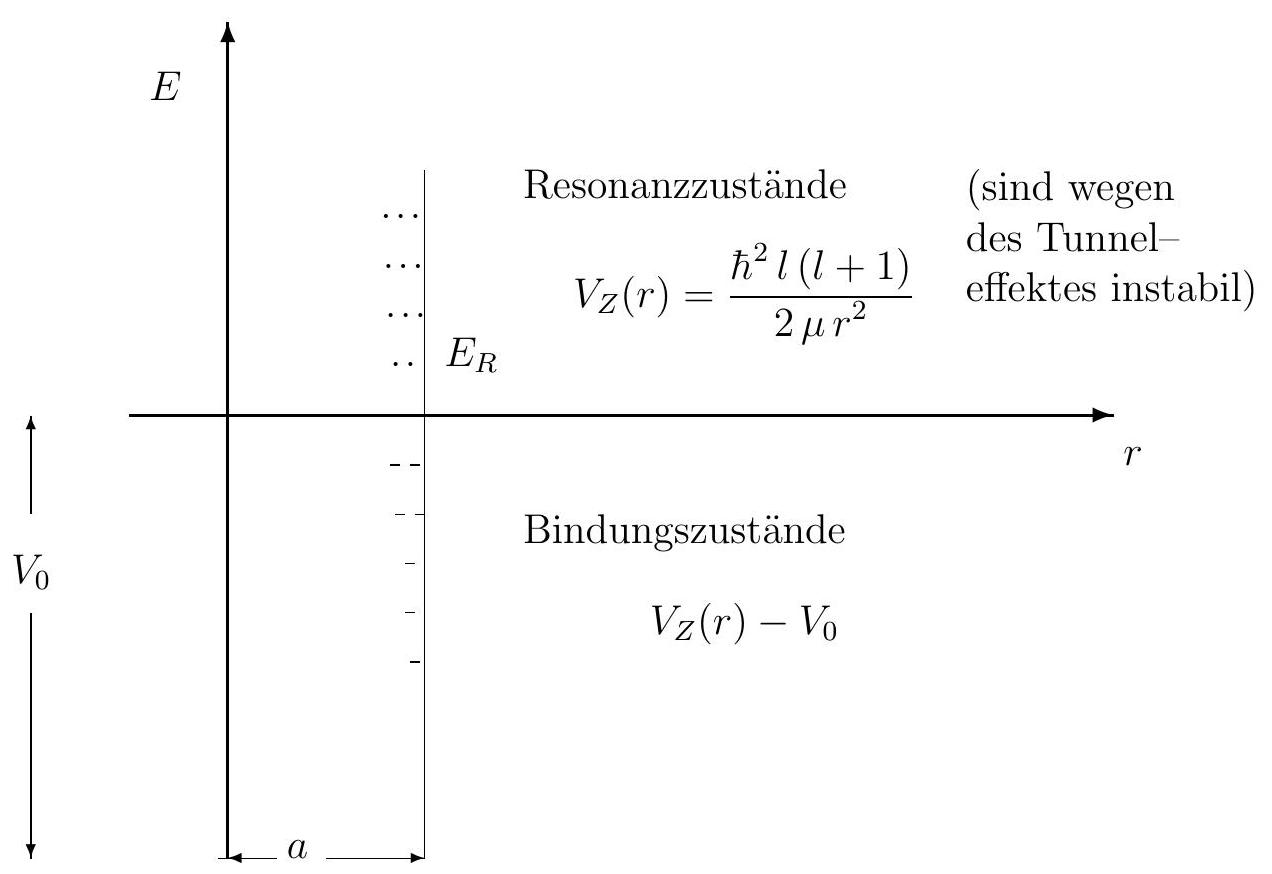
\includegraphics[scale=0.2]{2025_05_21_d5590f158a899e385c7cg-21}
\end{center}

---

\textbf{Breit-Wigner-Formel für Resonanzprofil [Definition]}

Nähern wir $\tan \delta_l$ bei $E \approx E_R$ durch:

\[
\tan \delta_l \approx \gamma_l \frac{(ka)^{2l+1}}{E - E_R}
\]

Dann gilt:

\[
\sigma_l(E) = \frac{4\pi(2l+1)}{k^2} \cdot \frac{(\gamma_l(ka)^{2l+1})^2}{(E - E_R)^2 + (\gamma_l(ka)^{2l+1})^2}
\]

Dies ist die \textbf{Breit-Wigner-Formel} für den Wirkungsquerschnitt in Resonanznähe.

---

\textbf{Resonanzbreite und komplexe Amplitude [Definition]}

Die Partialwellenamplitude:

\[
f_l(k) = \frac{1}{2ik} (e^{2i\delta_l} - 1) =
\frac{1}{k} \cdot \frac{\tan \delta_l}{1 - i \tan \delta_l}
\]

Setzt man $\tan \delta_l$ aus der Breit-Wigner-Näherung ein, erhält man:

\[
f_l(k) = \frac{1}{k} \cdot \frac{\gamma_l (ka)^{2l+1}}{E - E_R - i \gamma_l (ka)^{2l+1}}
\]

Die Resonanzbreite ist definiert durch:

\[
\Gamma_l = 2 \gamma_l (ka)^{2l+1}
\]

Dann ist:

\[
\sigma_l(E_R \pm \tfrac{1}{2} \Gamma_l) = \tfrac{1}{2} \sigma_l(E_R)
\]

\begin{center}
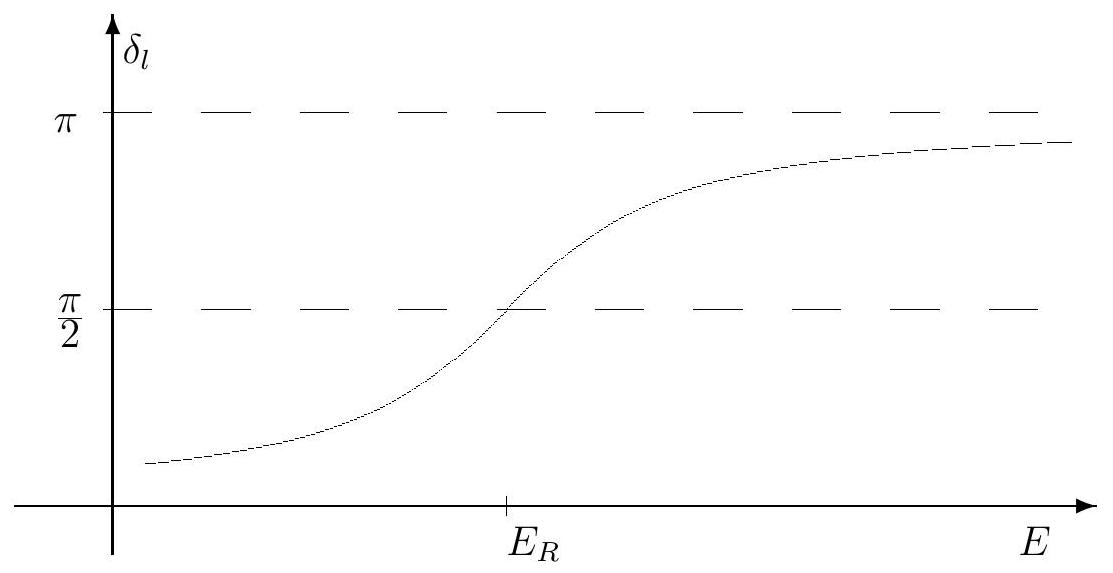
\includegraphics[scale=0.2]{2025_05_21_d5590f158a899e385c7cg-22}
\end{center}






\pagebreak


\subsubsection*{Schrödinger-Gleichung für rotationssymmetrische Potentiale}

\subsubsection*{Drehimpulserhaltung}
Für ein rotationssymmetrisches Potential $V(\vec{x})=V(|\vec{x}|)$ ist der Hamiltonian invariant unter Rotationen. Klassisch wie quantenmechanisch ist der Drehimpuls eine gute Quantenzahl. Es gilt

$$
\left[\mathbf{L}_{j}, \mathbf{H}\right]=0, \quad j=1,2,3, \quad \text { also auch } \quad\left[\overrightarrow{\mathbf{L}}^{2}, \mathbf{H}\right]=0
$$

Wie wir später noch sehen werden, ist ein Operator genau dann eine Erhaltungsgrösse, wenn er mit dem Hamiltonoperator vertauscht. Aus Abschnitt ?? wissen wir: Vertauschen zwei Operatoren, kann man sie gleichzeitig auf Diagonalform bringen. Dies bedeutet:

\begin{itemize}
  \item Man kann die Eigenfunktionen von
\end{itemize}

$$
\mathbf{H}=\frac{\overrightarrow{\mathbf{p}}^{2}}{2 m}+V(r)
$$

gleichzeitig als Eigenfunktionen zu $\overrightarrow{\mathbf{L}}^{2}$ und $\mathbf{L}_{3}$ wählen.\\
Beweis\\
Wir benutzen

$$
[A B, C]=A[B, C]+[A, C] B \quad[A B, C]=A B C-C A B
$$

um $\left[\mathbf{L}_{i}, \overrightarrow{\mathbf{p}}^{2}\right]=0$ nachzuvollziehen, sowie $\overrightarrow{\mathbf{p}}^{2}=p_{l} p_{l}$ :

$$
\begin{aligned}
\epsilon_{i j k}\left[x_{j} p_{k}, p_{l} p_{l}\right] & =\epsilon_{i j k}\left(x_{j}\left[p_{k}, p_{l} p_{l}\right]+\left[x_{j}, p_{l} p_{l}\right] p_{k}\right)=-\epsilon_{i j k}\left[p_{l} p_{l}, x_{j}\right] p_{k} \\
& =-\epsilon_{i j k}\left(p_{l}\left[p_{l}, x_{j}\right]+\left[p_{l}, x_{j}\right]\right) p_{k} \\
& =i \hbar \epsilon_{i l k}\left(p_{l}+p_{k}\right)
\end{aligned}
$$

Wegen $\epsilon_{i l k}=-\epsilon_{i k l}$ verschwindet der letzte Term.

In Bezug auf das Potential genügt die Bemerkung, dass die Komponenten des Drehimplusoperators mit jeder Operator-Funktion trivialerweise vertauschen, wenn diese nur von $r$ abhängt. Man betrachte z.B. $L_{3}=(\hbar / i) \partial_{\varphi}$.

\subsubsection*{Hamilton-Operator in Kugelkoordinaten}
Der Laplace-Operator lautet in sphärischen Koordinaten

$$
\begin{aligned}
\Delta & =\frac{1}{r^{2}} \frac{\partial}{\partial r}\left(r^{2} \frac{\partial}{\partial r}\right)+\frac{1}{r^{2} \sin ^{2} \vartheta}\left(\sin \vartheta \frac{\partial}{\partial \vartheta} \sin \vartheta \frac{\partial}{\partial \vartheta}+\frac{\partial^{2}}{\partial \varphi^{2}}\right) \\
& =\frac{1}{r} \frac{\partial^{2}}{\partial r^{2}} r-\frac{1}{r^{2} \hbar^{2}} \overrightarrow{\mathbf{L}}^{2}
\end{aligned}
$$

Die Herleitung ist länglich, ansonsten aber elementar. Der erste Term in der zweiten Gleichung ist lediglich eine alternative Darstellung, ${ }^{1}$ für den zweiten Term vergleiche Abschnitt ??. Der Ausgangspunkt unserer Überlegungen ist damit

$$
H=-\frac{\hbar^{2}}{2 r m_{0}} \frac{\partial^{2}}{\partial r^{2}} r+\frac{1}{2 m_{0} r^{2}} \overrightarrow{\mathbf{L}}^{2}+V(r)
$$

\subsubsection*{Entwicklung nach Kugelfunktionen}
Sei $u(\vec{x})$ eine Lösung der zeitunabhängigen Schrödinger-Gleichung. Wir entwickeln den Winkelanteil nach Kugelfunktionen $Y_{l m}$ :

$$
u(\vec{x})=\sum_{l=0}^{\infty} \sum_{m=-l}^{m=+l} R_{l m}(r) Y_{l m}(\vartheta, \varphi), \quad r=|\vec{x}|
$$

Damit wird die Schrödinger-Gleichung zu

$$
\begin{array}{r}
\sum_{l=0}^{\infty} \sum_{m=-l}^{m=+l}\left[-\frac{\hbar^{2}}{2 r m_{0}} \frac{\partial^{2}\left(r R_{l m}\right)}{\partial r^{2}}+\frac{\hbar^{2} l(l+1)}{2 m_{0} r^{2}} R_{l m}(r)+V(r) R_{l m}(r)\right] Y_{l m}(\vartheta, \varphi) \\
=E \sum_{l=0}^{\infty} \sum_{m=-l}^{m=+l} R_{l m}(r) Y_{l m}(\vartheta, \varphi)
\end{array}
$$

Multipliziert man diese Gleichung mit $Y_{l^{\prime} m^{\prime}}^{*}$ und integriert über $\vartheta$ und $\varphi$, so folgt wegen $\left(Y_{l_{1} m_{1}}, Y_{l_{2} m_{2}}\right)=\delta_{l_{1} l_{2}} \delta_{m_{1} m_{2}}$ für $R_{l m}(r)$ die Gleichung

$$
-\frac{\hbar^{2}}{2 r m_{0}} \frac{\partial^{2}\left(r R_{l m}\right)}{\partial r^{2}}+\left[\frac{\hbar^{2} l(l+1)}{2 m_{0} r^{2}}+V(r)\right] R_{l m}(r)=E R_{l m}(r)
$$

\subsubsection*{Zentrifugalpotential}
Im folgenden wird angenommen, daß das Zentrifugalpotential

$$
\frac{\hbar^{2} l(l+1)}{2 m r^{2}}
$$

\footnotetext{${ }^{1}(1 / r) \partial_{r}^{2} r=2 / r+\partial_{r}^{2}=\left(1 / r^{2}\right) \partial_{r}\left(r^{2} \partial_{r}\right)$.
}
für $l \neq 0$ und $r \rightarrow 0$ gegenüber $V(r)$ dominiert, d.h. dass
$$
\lim _{r \rightarrow 0}\left(r^{2} V(r)\right)=0
$$
gilt, wie es für das Coulomb-Potential der Fall ist. Anschaulich bedeutet dieses, daß auch quantenmechanisch das Teilchen nicht in den Ursprung "fallen" soll, die Wahrscheinlichkeitsdichte
$$
w(\vec{x})=u^{*}(\vec{x}) u(\vec{x})
$$
für $\vec{x} \rightarrow 0$ also endlich bleibt, d.h. $R_{l m}(r=0)$ soll endlich sein.

\subsubsection*{Verhalten für $r \rightarrow 0$}
Für $r \rightarrow 0$ kann man $E$ und $V(r)$ gegenüber $r^{-2}$ vernachlässigen:

$$
-\frac{d^{2}}{d r^{2}}\left(r R_{l m}(r)\right)-\frac{l(l+1)}{r^{2}} R_{l m}(r) \approx 0, \quad \text { für } \quad r \rightarrow 0 .
$$

Die Lösungen sind

$$
R_{l m}(r) \approx C r^{\nu}, \quad \nu(\nu+1)=l(l+1) ; \quad \quad \nu=l, \quad \text { oder } \quad \nu=-l-1
$$

Wenn $R_{l m}(r=0)<\infty$, kommt nur die reguläre Lösung $\nu=l$ in Frage

\subsection*{Die Bindungszustände des Wasserstoffatoms}
Es sei nun

$$
V(r)=-\frac{Z e_{0}^{2}}{4 \pi \varepsilon_{0} r}
$$

das Potential für ein Elektron mit Ladung $-e_{0}$ im Feld eines Kernes mit Ladung $Z e_{0}$. Mit $R_{l m}(r) \equiv R(r)$ wird die Schrödingergleichung für die radiale Wellenfunktion zu

$$
\left(\frac{d^{2}}{d r^{2}}+\frac{2}{r} \frac{d}{d r}\right) R+\frac{2 m_{0}}{\hbar^{2}}\left[E+\frac{Z e_{0}^{2}}{4 \pi \varepsilon_{0} r}-\frac{\hbar^{2} l(l+1)}{2 m_{0} r^{2}}\right] R(r)=0
$$

Gesucht werden quadratintegrierbare Lösungen mit $E<0$ (gebundene Zustände).

\subsubsection*{Dimensionslose Variablen}
Führt man die neuen Variablen

$$
\begin{aligned}
& \rho=\left(\frac{8 m_{0}|E|}{\hbar^{2}}\right)^{\frac{1}{2}} r, \lambda=Z \alpha\left(\frac{c^{2} m_{0}}{2|E|}\right)^{\frac{1}{2}} \\
& \alpha=\frac{e_{0}^{2}}{4 \pi \varepsilon_{0} \hbar c} \approx \frac{1}{137}: \text { Sommerfeldsche } \\
& \text { Feinstrukturkonstante }
\end{aligned}
$$

ein, so erhält man die radiale Schrödingergleichung

$$
\frac{d^{2} R}{d \rho^{2}}+\frac{2}{\rho} \frac{d R}{d \rho}+\left(\frac{\lambda}{\rho}-\frac{1}{4}-\frac{l(l+1)}{\rho^{2}}\right) R=0
$$

Die Kontrolparameter sind der Drehimplus $l(l+1)$ und $\lambda$.

\subsubsection*{Verhalten für $r \rightarrow \infty$}
Für große $\rho$ ergibt sich für $R \sim R_{\infty}(\rho)$ näherungsweise

$$
\frac{d^{2} R_{\infty}}{d \rho^{2}}-\frac{1}{4} R_{\infty}=0, \quad R_{\infty} \sim e^{ \pm \rho / 2}
$$

Als normierbare Lösung kommt nur $e^{-\rho / 2}$ in Frage.

\subsubsection*{Allgemeine Lösung}
Wir hatten bereits gezeigt, daß $R(\rho) \sim \rho^{l}$ für $\rho \rightarrow 0$ gilt. Daher betrachten wir nun den Ansatz

$$
R(\rho)=\rho^{l} e^{-\rho / 2} g(\rho)
$$

Hiermit finden wir für $g(\rho)$ die Gleichung

$$
\frac{d^{2} g(\rho)}{d \rho^{2}}+\left(\frac{2 l+2}{\rho}-1\right) \frac{d g}{d \rho}+\frac{\lambda-1-l}{\rho} g(\rho)=0
$$

\subsubsection*{Taylor-Entwicklung}
Wir entwickeln die Lösung in eine Taylorreihe in $\rho$,

$$
g(\rho)=\sum_{n=0}^{\infty} a_{n} \rho^{n}
$$

und setzen sie ein. Wir finden

$$
\sum_{n=0}^{\infty}\left[n(n-1) a_{n} \rho^{n-2}+\left(\frac{2 l+2}{\rho}-1\right) n a_{n} \rho^{n-1}+(\lambda-1-l) a_{n} \rho^{n-1}\right]=0
$$

bzw.

$$
\sum_{n=0}^{\infty}\left[(n+1)\left(n a_{n+1}+(2 l+2) a_{n+1}\right)+(\lambda-1-l-n) a_{n}\right] \rho^{n-1}=0
$$

Da diese Gleichung für alle $\rho$ gelten soll, müssen die Koeffizienten einzeln verschwinden:

$$
a_{n+1}=\frac{n+l+1-\lambda}{(n+1)(n+2 l+2)} a_{n}
$$

Bricht die Reihe nicht ab, so hätte man für große $n: a_{n+1} \sim \frac{1}{(n+1)} a_{n}$, d.h. $g(\rho)$ verhielte sich für große $\rho$ wie

$$
g(\rho) \sim e^{\rho}
$$

Dies würde jedoch zu einem nicht normierbaren $R(\rho)$ führen. Die Reihe muß für normierbare $R$ also abbrechen.

\subsubsection*{Hauptquantenzahl}
Es muß also ein $n=n_{r}$ geben, für welches $a_{n_{r}+1}=0$, d.h.

$$
\lambda=n_{r}+l+1, \quad n_{r} \geq 0
$$

\begin{center}
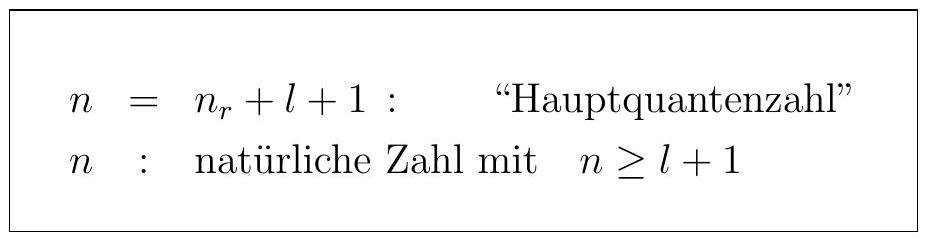
\includegraphics[scale=0.2]{2025_05_21_d5590f158a899e385c7cg-05}
\end{center}

Als muss $\lambda=Z \alpha \sqrt{\frac{c^{2} m_{0}}{2|E|}}$ eine ganze Zahl sein, $\lambda=n$. Hieraus folgt für die möglichen Energiewerte $E=E_{n}$ der gebundenen Zustände des Wasserstoffatoms:

$$
E_{n}=-\frac{1}{2} m_{0} c^{2} \frac{(Z \alpha)^{2}}{n^{2}} \quad \text { (Bohr'sche Formel) }
$$

\subsubsection*{Bahn-Quantenzahlen}
Die Abbruchbedingung

$$
a_{n_{r}+1}=0, \quad n-1=n_{r}+l
$$

hat für feste Hauptquantenzahl $n$ noch einen Freiheitsgrad,

$$
l=0,1, \ldots n-1
$$

Dieses sind die erlaubten Werte des Drehimpules.

\subsubsection*{Entartungsgrad}
Da zu $l$ schon $2 l+1$ Zustände mit verschiedenen $l_{3}$-Komponenten gehören, so ist der gesamte Entartungsgrad durch

$$
\sum_{l=0}^{n-1}(2 l+1)=n^{2}
$$

gegeben. Zu vorgegebenem $E_{n}$ gehören also $n^{2}$ verschiedene Bahndrehimpuls-Zustände. Berücksichtigt man außerdem, daß zu jedem Bahndrehimpuls-Zustand ( $l, m$ ) noch je 2 Spin-Zustände des Elektrons gehören, so bekommt man schließlich als Entartungsgrad von $E_{n}$ den Wert $d_{n}=2 n^{2}$. Dies ist die Dimension des zu $E_{n}$ gehörigen Unterraumes.

$$
d_{1}=2, \quad d_{2}=8, \quad d_{3}=18 \quad \text { etc. }
$$

Dieses Ergebnis ist für die Atomphysik wichtig.

\subsubsection*{Eigenfunktionen des Wasserstoffatoms}
Die Funktionen $g(\rho)$ sind Polynome vom Grad $n_{r}=n-l-1$, mit $n_{r}=0,1, \ldots$ Für gegebene $n$ und $l$ gilt die Rekursionsformel für die Koeffizienten $a_{\nu}$,

$$
a_{\nu+1}=\frac{\nu+l+1-n}{(\nu+1)(\nu+2 l+2)} a_{\nu} \quad \nu=0, \ldots n_{r}
$$

wobei $n_{r}=n-l-1$. Bei geeigneter Wahl von $a_{0}$ sind die Polynome identisch mit denn sogenannten zugeordneten Laguerre'schen Polynomen:

$$
\begin{aligned}
L_{n_{r}}^{\alpha}(\rho) & =\sum_{\nu=0}^{n_{r}}(-1)^{\nu}\binom{n_{r}+\alpha}{n_{r}-\nu} \frac{\rho^{\nu}}{\nu!} \\
& =\frac{1}{n_{r}!} e^{\rho} \rho^{-\alpha} \frac{d^{n_{r}}}{d \rho^{n_{r}}}\left(e^{-\rho} \rho^{n_{r}+\alpha}\right)
\end{aligned}
$$

Für $\alpha=0$ erhält man die Laguerre'schen Polynome. Für das Wasserstoffatom gilt $\alpha=$ $2 l+1$.

\subsubsection*{Beispiele}
Die radialen Eigenfunktionen $R_{n l m}(\rho) \equiv R_{n l}(\rho)$ des Wasserstoffatoms mit Energie $E_{n}$ sind

$$
R_{n l}(\rho)=C_{n l} e^{-\frac{1}{2} \rho} \rho^{l} L_{n-l-1}^{2 l+1}(\rho)
$$

wobei $C_{n l}$ der Normierungsfaktor ist. Setzt man

$$
a \equiv \frac{\hbar^{2} 4 \pi \varepsilon_{0}}{m_{e} e^{2}} \quad: \text { Bohr'scher Atomradius }
$$

so hat man z.B. (normiert)

$$
\begin{aligned}
& R_{10}(r)=2\left(\frac{Z}{a}\right)^{3 / 2} e^{-Z r / a} \\
& R_{20}(r)=2\left(\frac{Z}{2 a}\right)^{3 / 2}\left(1-\frac{Z r}{2 a}\right) e^{-Z r /(2 a)} \\
& R_{21}(r)=\frac{1}{\sqrt{3}}\left(\frac{Z}{2 a}\right)^{3 / 2} \frac{Z r}{a} e^{-Z r /(2 a)}
\end{aligned}
$$

\subsubsection*{Aufenthaltswahrscheinlichkeit}
Die Wahrscheinlichkeit, das Elektron in einer Kugelschale mit Radius $r$ und $r+\Delta r$ anzutreffen, ist durch

$$
w(\Delta r)=\int_{r}^{r+\Delta r} d r w_{n l}(r), \quad w_{n l}(r)=r^{2} R_{n l}^{2}(r)
$$

gegeben. Das Maximum der Aufenthaltswahrscheinlichkeit liegt für $w_{10}(r)=C_{10}^{2} r^{2} e^{-2 Z r} / a$ bei $r=a / Z$. Im allgemeinen hat $w_{n l}(r)$ genau $n-l$ Maxima.

Die Mittelwerte $<r^{k}>=\int_{0}^{\infty} d r r^{k} w_{n l}(r)$ lassen sich für $k= \pm 1$ einfach berechnen:

$$
<r>=\frac{a}{2 Z}\left[3 n^{2}-l(l+1)\right], \quad<r^{-1}>=\frac{Z}{a n^{2}}
$$

\subsubsection*{Korrekturen}
Die Bohr'sche Formel für die Energieniveaus des Elektrons im Wasserstoffatom stellt nur eine Näherung dar, zu der eine ganze Reihe von Korrekturen kommen (Feinstruktur, Hyperfeinstruktur etc).

\subsubsection*{Mitbewegung des Kernes}
Wir haben bisher so getan, als ob der Kern des Wasserstoffatoms unendlich schwer sei (und deshalb ruht). Tatsächlich haben Kern und Elektron die Masse

$$
c^{2} m_{p}=938 \mathrm{MeV}, \quad c^{2} m_{e}=0.51 \mathrm{MeV}
$$

und seine Mitbewegung macht sich bemerkbar.\\
Die Energie $\tilde{E}$ zweier Teilchen mit Koordinaten $\vec{x}_{i}=\left(x_{1}^{(i)}, x_{2}^{(i)}, x_{3}^{(i)}\right), i=1,2$, und wechselseitigem Potential $V\left(\vec{x}_{1}-\vec{x}_{2}\right)$ ist klassisch durch

$$
\tilde{E}=\frac{1}{2 m_{1}} \vec{p}_{1}^{2}+\frac{1}{2 m_{2}} \vec{p}_{2}^{2}+V\left(\vec{x}_{1}-\vec{x}_{2}\right)
$$

gegeben. Das Äquvalenzprinzip,

$$
\vec{p}_{1} \rightarrow \frac{\hbar}{i} \operatorname{grad}_{1}, \quad \vec{p}_{2} \rightarrow \frac{\hbar}{i} \operatorname{grad}_{2}, \quad \operatorname{grad}_{j}=\left(\frac{\partial}{\partial x_{1}^{(j)}}, \frac{\partial}{\partial x_{2}^{(j)}}, \frac{\partial}{\partial x_{3}^{(j)}}\right)
$$

führt zu der stationären Schrödinger-Gleichung für zwei Teilchen:

$$
\left(-\frac{\hbar^{2}}{2 m_{1}} \Delta_{1}-\frac{\hbar^{2}}{2 m_{2}} \Delta_{2}+V\left(\vec{x}_{1}-\vec{x}_{2}\right)\right) \tilde{u}\left(\vec{x}_{1}, \vec{x}_{2}\right)=\tilde{E} \tilde{u}\left(\vec{x}_{1}, \vec{x}_{2}\right)
$$

\subsubsection*{Schwerpunktskoordinaten}
Mittels Relativ- und Schwerpunktkoordinaten

$$
\begin{aligned}
\vec{x} & =\vec{x}_{1}-\vec{x}_{2}, & \vec{R}=\frac{\left(m_{1} \vec{x}_{1}+m_{2} \vec{x}_{2}\right)}{\left(m_{1}+m_{2}\right)} & \\
\vec{x}_{1} & =\vec{R}+\frac{\mu}{m_{1}} \vec{x}, & \vec{x}_{2}=\vec{R}-\frac{\mu}{m_{2}} \vec{x}, & \mu=\frac{m_{1} m_{2}}{m_{1}+m_{2}}
\end{aligned}
$$

wird die Kern-Elektron Schrödingergleichung zu

$$
\left(-\frac{\hbar^{2}}{2\left(m_{1}+m_{2}\right)} \Delta_{R}-\frac{\hbar^{2}}{2 \mu} \Delta_{x}+V(\vec{x})\right) \tilde{u}(\vec{x}, \vec{R})=\tilde{E} \tilde{u}(\vec{x}, \vec{R})
$$

die man auch herleiten kann, indem man das Äquivalenzprinzip direkt auf Relativ- und Schwerpunkts-Koordinaten anwendet. Hier is $m_{1}+m_{2}$ die Gesamtmasse und $\mu=m_{1} m_{2} /\left(m_{1}+\right.$ $m_{2}$ ) die Relativmasse, wie schon aus der Mechanik bekannt.

\subsubsection*{Seperation der Variablen}
Als Separation der Variablen nennt man Produkt-Ansätze für die Lösung von Differentialgleichungen, wie $\psi(\vec{x}, t)=u(\vec{x}) \exp (i E t / \hbar)$. Der analoge Ansatz für Relativ- und Schwerpunkts-Koordinaten ist

$$
\tilde{u}(\vec{x}, \vec{R})=u(\vec{x}) u(\vec{R}), \quad u(\vec{R})=e^{i \vec{K} \cdot \vec{R}}
$$

wobei wir davon Gebrauch gemacht haben, daß der der Gesamptimpuls $\vec{p}_{1}+\vec{p}_{2}$ erhalten ist, d.h. dass sich die Schwerpunktskoordinate frei bewegt (als ebene Welle). Die Schrödingergleichung für die Relativ-Koordinate ist damit

$$
\left(-\frac{\hbar^{2}}{2 \mu} \Delta_{x}+V(\vec{x})\right) u(\vec{x})=E u(\vec{x}), \quad E=\tilde{E}-\frac{\hbar^{2} \vec{K}^{2}}{2\left(m_{1}+m_{2}\right)}
$$

Dabei ist

$$
\begin{aligned}
\frac{\hbar^{2} \vec{K}^{2}}{2\left(m_{1}+m_{2}\right)} & : \text { kinetische Energie des Schwerpunktes } \\
E & : \text { Energie der Relativbewegung }
\end{aligned}
$$

Die Schrödinger-Gleichung für die Relativbewegung ist also die gleiche wie für die Bewegung in einem äußeren Potential $V(\vec{x})$. Man hat lediglich die Masse $m$ durch die reduzierte Masse $\mu=m_{1} m_{2} /\left(m_{1}+m_{2}\right)$ zu ersetzen.

\subsubsection*{Energieniveaus}
Die Energie-Niveaus des Wasserstoffatoms ist somit

$$
E_{n}=-\frac{1}{2} \mu c^{2} \frac{\alpha^{2}}{n^{2}}, \quad \mu=\frac{m_{e}}{1+m_{e} / m_{p}}
$$

Geht man vom Proton zum Deuteron über, so hat man $m_{p} \rightarrow m_{d} \approx 2 m_{p}$ und eine entsprechende Verschiebung der Energieniveaus des schwerer Wasserstoffs. Aufgrund dieses Effektes wurde das Deuteron entdeckt. Eine Reihe weiterer physikalischer Effekte führen zu Korrekturen der Bohr'schen Energieniveaus.

\begin{itemize}
  \item Das magnetischen Moment des Elektrons.
  \item Relativistischen Geschwindigkeit des Elektrons.
  \item Das magnetischen Moment des Kerns.
\end{itemize}

\subsection*{Radialsymmetrische Lösungen für $V(r)=0$}
Die Lösungen der freien Schrödinger-Gleichung lassen sich in verschiedenen Systemen von Basisfunktionen darstellen. Bisher haben wir dazu ebenen Wellen verwendet, die Eigenfunktionen des Impulsoperators.

Hier betrachten wir Lösungen der Form $R_{l m}(r) Y_{l m}(\vartheta, \varphi)$, welche bei Streuprozessen auftreten. Zunächst beschäftigen wir uns mit der Lösung für die radialen Wellenfunktionen, $R_{l m}(r)$. und schreiben kurz $R_{l m}(r) \equiv R_{l}(r)$. Für $V \equiv 0$ hat die radiale Schrödingergleichung die Form

$$
-\frac{\hbar^{2}}{2 m r} \frac{\partial^{2}\left(r R_{l}\right)}{\partial r^{2}}+\frac{\hbar^{2} l(l+1)}{2 m r^{2}} R_{l}(r)=E R_{l}(r)
$$

Da diese freie Teilchen beschreibt, sind die Energie-Eigenwerte kontinuierlich, aber positiv, $E \geq 0$.

\subsubsection*{Sphärische Bessel- und Neumann-Funktionen}
Es gibt verschiedene Wege, dimensionslose Variable für die radiale Schrödingergleichung einzuführen, eine Möglichkeit haben wir auf Seite 4 im Zusammenhang mit der Diskussion gebundener Zustände benutzt. Hier setzen wir

$$
\frac{2 m E}{\hbar^{2}}=k^{2}=|\vec{k}|^{2}, \quad \text { und } \quad \rho \equiv k r
$$

Damit erhalten wir

$$
\frac{d^{2} R_{l}}{d \rho^{2}}+\frac{2}{\rho} \frac{d R_{l}}{d \rho}-\frac{l(l+1)}{\rho^{2}} R_{l}+R_{l}=0
$$

Man beachte, daß die Energie $\hbar^{2} k^{2} /(2 m)$ nur via der Reskalierung des radialen Abstandes eingeht, via $\rho=k r$. Als Differentialgleichung 2. Ordnung hat diese Gleichung zwei unabhängige Lösungen, welche man auch "sphärischen Zylinderfunktionen" nennt.

\subsubsection*{Bessel-Funktion}
Die Lösungen der radialen Schrödinger-Gleichung stehen in einem engen Zusammenhang mit den Bessel-Funktionen $J_{\nu}(\rho)$ :

$$
\begin{aligned}
0 & =\frac{d^{2} J_{\nu}}{d \rho^{2}}+\frac{1}{\rho} \frac{d J_{\nu}}{d \rho}+\left(1-\frac{\nu^{2}}{\rho^{2}}\right) J_{\nu}(\rho) \\
J_{\nu}(\rho) & =\frac{\rho^{\nu}}{2^{\nu}} \sum_{k=0}^{\infty}(-1)^{k} \frac{\rho^{2 k}}{2^{2 k} k!\Gamma(\nu+k+1)}
\end{aligned}
$$

Diese werden überall da gebraucht, wo es um Lösungen der Laplace Gleichung in polaroder sphärischen Koordinaten geht. Dabei kann $\nu$ complex sein.

\subsubsection*{Sphärische Bessel-Funktion}
Wir betrachten nun die bei $\rho=0$ reguläre Lösung, die sphärische Bessel-Funktion $j_{\nu}(\rho)$ :

$$
j_{l}(\rho)=\left(\frac{\pi}{2 \rho}\right)^{\frac{1}{2}} J_{l+\frac{1}{2}}(\rho), \quad j_{l}(\rho)=(-\rho)^{l}\left(\frac{1}{\rho} \frac{d}{d \rho}\right)^{l}\left(\frac{\sin \rho}{\rho}\right)
$$

Aus der zweiten Darstellung folgt

$$
j_{0}(\rho)=\frac{\sin \rho}{\rho}, \quad j_{1}(\rho)=\frac{\sin \rho}{\rho^{2}}-\frac{\cos \rho}{\rho}
$$

Man kann durch vollständige Induktion verifizieren, dass die $j_{l}(\rho)$ Lösungen der radialen Schrödingergleichung sind. D.h. man beweist zunächst den Fall $l=0$ und schliesst dann aus der Richtigkeit für $l$ auf die Richtigkeit für $l+1$.

\subsubsection*{Sphärische Neumann-Funktionen}
Wir betrachten nun die bei $\rho=0$ singuläre Lösung, die sphärische Neumann-Funktionen $n_{l}(\rho)$ :

$$
n_{l}(\rho)=(-1)^{l+1}\left(\frac{\pi}{2 \rho}\right)^{\frac{1}{2}} J_{-l-\frac{1}{2}}(\rho), \quad n_{l}(\rho)=-(-\rho)^{l}\left(\frac{1}{\rho} \frac{d}{d \rho}\right)^{l}\left(\frac{\cos \rho}{\rho}\right)
$$

Mit

$$
n_{0}(\rho)=-\frac{\cos \rho}{\rho}, \quad n_{1}(\rho)=-\frac{\cos \rho}{\rho^{2}}-\frac{\sin \rho}{\rho}
$$

\subsubsection*{Grenzwertverhalten}
Für $\rho \rightarrow 0$ gilt

$$
\begin{aligned}
& j_{l}(\rho) \approx \frac{\rho^{l}}{(2 l+1)!!} \quad(2 l+1)!!\equiv 1 \cdot 3 \cdot 5 \cdots(2 l+1) \\
& n_{l}(\rho) \approx \frac{-(2 l-1)!!}{\rho^{l+1}}
\end{aligned}
$$

Für $\rho \rightarrow \infty$ gilt andererseits

$$
j_{l}(\rho) \sim \frac{1}{\rho} \sin \left(\rho-\frac{l \pi}{2}\right), \quad n_{l}(\rho) \sim-\frac{1}{\rho} \cos \left(\rho-\frac{l \pi}{2}\right)
$$

\subsubsection*{Entwicklung von ebenen Wellen nach Legendre-Polynomen}
Ebene Wellen,

$$
e^{i \vec{k} \cdot \vec{x}}=e^{i k r \cos \vartheta}=e^{i \rho z}, \quad \vartheta=\angle(\vec{k}, \vec{x}), \quad \rho=k r, \quad z \cos \vartheta,
$$

sind reguläre Lösungen von $\left(\Delta+k^{2}\right) u(\vec{x})=0$, sie lassen sich daher ebenfalls nach Kugelfunktionen und sphärischen Bessel-Funktionen $j_{l}(\rho)$ entwickeln.

Eine ebene Welle hängt von der Energie $\hbar^{2} k^{2} /(2 m)$ nur via der Reskalierung des radialen Abstandes $\rho=k r \mathrm{ab}$, sie ist zudem rotations-invariant um die Ausbreitungsrichtung $\vec{k}=(0,0, k)$, und damit unabhängig vom Polarwinkel $\varphi$. In der Entwicklung nach Kugelfunktionen $Y_{l m}(\varphi, \vartheta)$ treten daher nur die Terme $m=0$ auf, und damit nur die Legendre Polynome

$$
P_{l}(z)=\left(\frac{4 \pi}{2 l+1}\right)^{1 / 2} Y_{l 0}, \quad z=\cos \vartheta
$$

also

$$
e^{i \rho z}=\sum_{l=0}^{\infty} c_{l} j_{l}(\rho) P_{l}(z)
$$

Der radiale Anteil ist durch die sphärische Besselfunktion $j_{l}(\rho)$ gegeben, da diese die für $\rho \rightarrow 0$ regulär sind.

\subsubsection*{Entwicklungskoeffizienten}
Es bleiben die Entwicklungskoeffizienten $c_{l}$ mit Hilfe der Orthogonalitätsrelationen

$$
\int_{-1}^{+1} d z P_{l_{1}}(z) P_{l_{2}}(z)=\frac{2 \delta_{l_{1} l_{2}}}{\left(2 l_{1}+1\right)}, \quad c_{l} j_{l}(\rho)=\frac{2 l+1}{2} \int_{-1}^{+1} d z P_{l}(z) e^{i \rho z}
$$

für Legendre-Polynome zu bestimmen. Wenn wir $z^{n}$ nach $P_{l}(z)$ entwicklen, so tragen nur Terme $l \leq n$ bei. Andererseits ist $P_{l}(z)$ orthogonal zu allen $P_{n}(z)$ mit $n \neq l$, daher gilt

$$
\int_{-1}^{+1} d z z^{n} P_{l}(z)=\left\{\begin{array}{cc}
0 & \text { für } n<l \\
\frac{2 l!}{(2 l+1)!!} & \text { für } n=l
\end{array}\right.
$$

Für $e^{i \rho z}=\sum_{n=0}^{\infty}(i \rho z)^{n} /(n!)$ finden wir daher

$$
\int_{-1}^{+1} d z P_{l}(z) e^{i \rho z}=\frac{2}{(2 l+1)!!}(i \rho)^{l}+O\left(\rho^{l+1}\right)
$$

Wir können jetzt den Grenzwert $\rho \rightarrow 0$ betrachten. Mit $j_{l}(\rho) \rightarrow \rho^{l} /(2 l+1)$ !! erhalten

$$
c_{l} j_{l}(\rho) \approx c_{l} \frac{\rho^{l}}{(2 l+1)!!} \approx \frac{(2 l+1)}{2} \frac{2(i \rho)^{l}}{(2 l+1)!!}+\ldots \quad \text { (höhere Potenzen in } \rho \text { ) }
$$

Ein Koeffizientenvergleich führt via

$$
c_{l}=(2 l+1) i^{l}
$$

zu dem zentralen Ergebnis

$$
e^{i \vec{k} \cdot \vec{x}}=e^{i k r \cos \vartheta}=\sum_{l=0}^{\infty}(2 l+1) i^{l} j_{l}(k r) P_{l}(\cos \vartheta)
$$

\subsubsection*{Physikalische Interpretation}
Das asymptotischen Verhaltens der spährischen Bessel Funktion $j_{l}(\rho)$ für große $\rho$ ist

$$
j_{l}(\rho) \sim \frac{1}{\rho} \sin \left(\rho-\frac{l \pi}{2}\right)=-\frac{1}{2 i k r}\left[e^{-i\left(k r-\frac{1}{2} l \pi\right)}-e^{i\left(k r-\frac{1}{2} l \pi\right)}\right]
$$

mit

$$
\begin{aligned}
& \frac{1}{r} e^{-i(\omega t+k r)} \quad: \text { ein-laufende Kugelwelle } \\
& \frac{1}{r} e^{-i(\omega t-k r)} \quad: \text { aus-laufende Kugelwelle }
\end{aligned}
$$

wobei $\omega=\hbar k^{2} /(2 m)$. Um ein- und auslaufende Wellen zu unterscheiden betrachtet man den Ort konstanter Phase, $\omega t+k r=0$. Die sphärische Besselfunktion $j_{l}(\rho)$ ist also für große Abstände ( $k r \gg 1$ ) eine Superposition von ein- und auslaufenden Kugelwellen. Der Drehimpuls $l$ geht nur via der Phasenverschiebung $l \pi / 2$ ein.

Beweis\\
Man bemerke, dass $\sin (\rho-l \pi / 2)$ je nach Quantenzahl $\pm \sin (\rho)$ entspricht ( $l$ gerade), bzw. $\pm \cos (\rho)$ (l ungerade). ${ }^{2}$ Das ist in Einklang mit

$$
j_{l}(\rho)=(-\rho)^{l}\left(\frac{1}{\rho} \frac{d}{d \rho}\right)^{l}\left(\frac{\sin \rho}{\rho}\right)=(-\rho)^{l}\left(\frac{1}{\rho} \frac{d}{d \rho}\right)^{l-1}\left(\frac{\cos \rho}{\rho}-\frac{\sin \rho}{\rho^{2}},\right)
$$

wobei der zweite Term für grosse $\rho$ verschindet.

\subsection*{Elastische Potentialstreuung}
\subsubsection*{Voraussetzung}
Für die Formulierung der Streutheorie brauchen wir die Annahme, dass sich die ungebundenen Lösungen der Schrödinger-Gleichung im Unendlichen wie ebene Wellen verhalten. Dazu muss das Potential $V(r)$ schnell genug für $r \rightarrow \infty$ abfallen, man kann zeigen, daß dies für

$$
\lim _{r \rightarrow \infty}(r V(r))=0,
$$

der Fall ist. Wir behandeln hier nicht die Streuung am Coulomb-Potential, die eine gesonderte Behandlung braucht.

\footnotetext{${ }^{2}$ Gemäß dem Ableitungs-Zyklus sin $\rightarrow \cos \rightarrow(-\sin ) \rightarrow(-\cos ) \rightarrow \sin$.
}
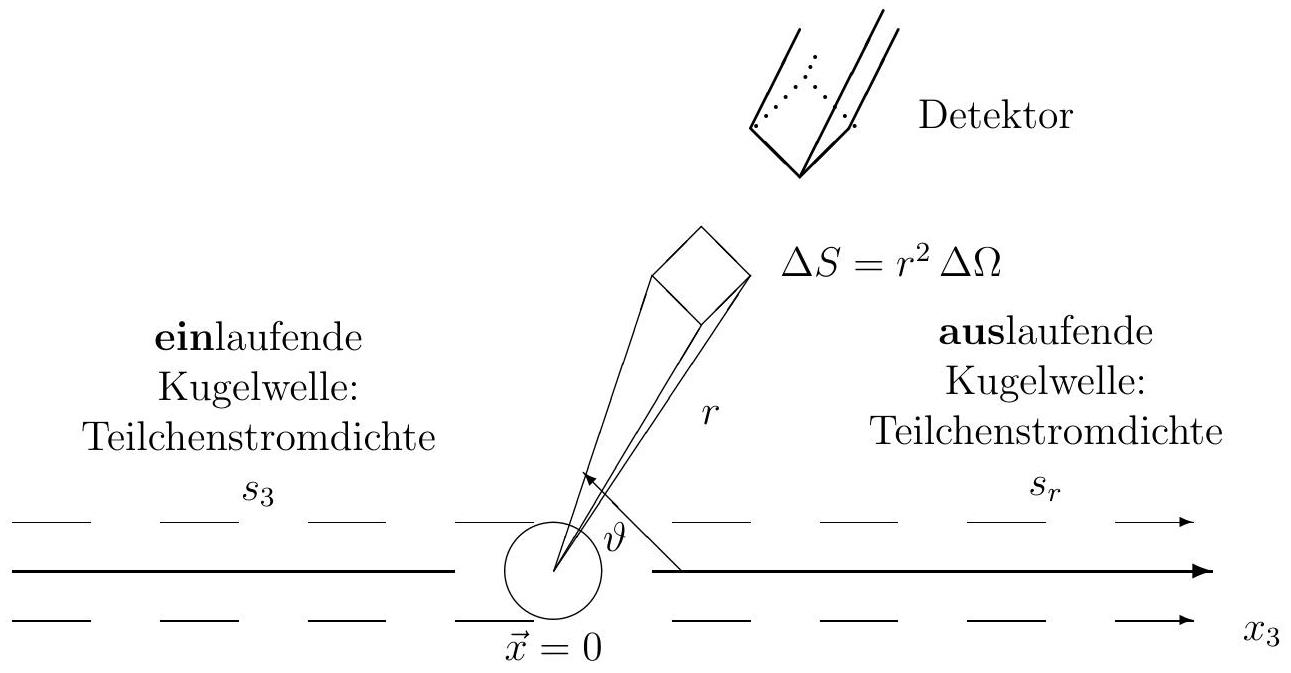
\includegraphics[scale=0.2, center]{2025_05_21_d5590f158a899e385c7cg-13}







\subsubsection*{Experimenteller Aufbau}
Längs der $x_{3}$-Achse fallen Teilchen der Stromdichte $s_{3}$ ein ${ }^{3}$ die am Streuzentrum in $\vec{x}=$ 0 (Relativkoordinate) in das Raumwinkelelement $\Delta \Omega$ mit radialer Teilchenstromdichte $s_{r}(r, \vartheta, \varphi)$ gestreut werden. Durch ein Flächenelement $\Delta S$ im Abstand $r$ treten dann pro Zeiteinheit $s_{r} \Delta S$ Teilchen.

Raumwinkelelement : $\Delta \Omega=\sin \vartheta \Delta \vartheta \Delta \varphi$

$$
\text { Fäschenelement : } \Delta S=r^{2} \Delta \Omega
$$

Stromdichte einfallender Teilchen : $s_{3}$\\
radiale Teilchenstromdichte : $\quad s_{r}(r, \vartheta, \varphi)=\vec{s} \cdot \vec{e}_{r}$

\subsubsection*{Wirkungsquerschnitt}
Der differentielle Wirkungsquerschnitt für die Streuung in das Raumwinkelelement $\Delta \Omega$ ist durch

$$
\begin{aligned}
\Delta \sigma(\vartheta, \varphi) & =\frac{s_{r} r^{2} \Delta \Omega}{s_{3}} \\
\frac{d \sigma}{d \Omega}(\vartheta, \varphi) & =\frac{s_{r}(r, \vartheta, \varphi) r^{2}}{s_{3}}
\end{aligned}
$$

definiert. Die Größe $d \sigma / d \Omega$ ist i.a. eine Funktion der Energie $E=\hbar^{2} k^{2} /(2 \mu)$, wobei $\mu$ die reduzierte Masse ist. Für rotationssymmetrische $V(\vec{x})$ hängt $d \sigma / d \Omega$ nicht von $\varphi \mathrm{ab}$.

\subsubsection*{Streuamplituden}
Sei $u(\vec{x})$ die Lösung der stationären Schrödinger-Gleichung zum Potential $V(r)$. Diese Lösung soll für große $r=|\vec{x}|$ aus einlaufender ebener Welle und auslaufender Kugelwelle

\footnotetext{${ }^{3}$ Vergleich den Abschnitt ?? zur Kontinuitätsgleichung.
}
bestehen,
$$
u(\vec{x}) \sim e^{i \vec{k} \cdot \vec{x}}+f(k, \vartheta) \frac{e^{i k r}}{r}, \quad \vec{k}=(0,0, k)
$$
mit $f(k, \vartheta)=0$ für $V(r)=0$. Die Größe $f(k, \vartheta)$ heißt Streuamplitude. Aus der Kontinuitätsgleichung folgt
$$
s_{3}=\hbar k_{3} / \mu, \quad s_{r}=\hbar k|f(k, \vartheta)|^{2} /\left(\mu r^{2}\right)
$$
und somit
$$
\frac{d \sigma(k, \vartheta)}{d \Omega}=\frac{s_{r} r^{2}}{s_{3}}=|f(k, \vartheta)|^{2}
$$
da $k_{3}=k$.

\subsubsection*{Entwicklung nach Partialwellen}
Die Partialwellen-Entwicklung ebener Wellen (siehe Abschnitt 5.3.2) reduziert sich für große $r$ zu

$$
\begin{aligned}
e^{i \vec{k} \cdot \vec{x}} & =\sum_{l=0}^{\infty}(2 l+1) i^{l} j_{l}(k r) P_{l}(\cos \vartheta) \\
& \sim-\frac{1}{2 i k} \sum_{l=0}^{\infty}(2 l+1) i^{l}\left(\frac{e^{-i\left(k r-\frac{1}{2} l \pi\right)}}{r}-\frac{e^{i\left(k r-\frac{1}{2} l \pi\right)}}{r}\right) P_{l}(\cos \vartheta)
\end{aligned}
$$

Diese ebene Welle entspricht dem Fall $V(r)=0$. Falls nun $V(r) \neq 0$, so wird lediglich die Amplitude/Phase der auslaufende Kugelwelle modifiziert. Wir machen den Ansatz

$$
u(\vec{x}) \approx-\frac{1}{2 i k} \sum_{l=0}^{\infty}(2 l+1) i^{l}\left(\frac{e^{-i\left(k r-\frac{1}{2} l \pi\right)}}{r}-S_{l}(k) \frac{e^{i\left(k r-\frac{1}{2} l \pi\right)}}{r}\right) P_{l}(\cos \vartheta)
$$

\subsubsection*{Streuphasen}
Bei einer rein elastischen Streuung können keine Teilchen verlorengehen, es werden also nur die Phasen, aber nicht jedoch die Intensitäten der auslaufenden Kugelwelle geändert werden. Also gilt $\left|S_{l}(k)\right|=1$ (bei inelastischer Streuung hat man $\left|S_{l}(k)\right|<1$ ), d.h.

$$
S_{l}(k)=e^{2 i \delta_{l}(k)}
$$

$$
\delta_{l}(k) \quad \text { : zur l-ten "Partialwelle" gehörige Streuphase. }
$$

Der Radialanteil $R_{l}(r)$ der Wellenfunktion verhält sich für große $r$ also asymptotisch wie

$$
R_{l}(r) \sim-\left(\frac{e^{-i\left(k r-\frac{1}{2} l \pi\right)}}{2 i k r}-e^{2 i \delta_{l}(k)} \frac{e^{i\left(k r-\frac{1}{2} l \pi\right)}}{2 i k r}\right)=e^{i \delta_{l}(k)} \frac{\sin \left(k r-\frac{1}{2} l \pi+\delta_{l}(k)\right)}{k r}
$$

\subsubsection*{Partialwellenentwicklung für Streuamplituden}
$\overline{\text { Mit } S_{l}=\left(S_{l}-1\right)+1 \text { läßt sich das obige } u(\vec{x}) \text { auch als }}$

$$
u(\vec{x}) \sim e^{i \vec{k} \cdot \vec{x}}+\left[\sum_{l=0}^{\infty}(2 l+1) i^{l} \frac{S_{l}(k)-1}{2 i k} P_{l}(\cos \vartheta) \frac{e^{i\left(k r-\frac{1}{2} l \pi\right)}}{r}\right]
$$

schreiben. Benutzen wir

$$
e^{-\frac{i}{2} l \pi}=i^{-l}, \quad u(\vec{x}) \sim e^{i \vec{k} \cdot \vec{x}}+f(k, \vartheta) \frac{e^{i k r}}{r}
$$

so erhält man für große $r$ mit

$$
f(k, \vartheta)=\sum_{l=0}^{\infty}(2 l+1) \frac{e^{2 i \delta_{l}(k)}-1}{2 i k} P_{l}(\cos \vartheta)
$$

Partialwellenentwicklung für die Streuamplituden $f(k, \vartheta)$.

\subsubsection*{Totaler Wirkungsquerschnitt}
Integrieren wir den differentiellen Wirkungsquerschnitt über die Einheitskugel, so erhalten wir den totalen elastischen Wirkungsquerschnitt $\sigma_{e l}(k)$ :

$$
\sigma_{e l}(k)=\int d \Omega|f(k, \vartheta)|^{2}
$$

Wegen der Orthogonalität der $P_{l}(\cos \vartheta)$ und da $\left(e^{2 i \delta_{l}}-1\right) / 2 i=e^{i \delta_{l}} \sin \delta_{l}$, folgt

$$
\sigma_{e l}(k)=\frac{4 \pi}{k^{2}} \sum_{l=0}^{\infty}(2 l+1) \sin ^{2} \delta_{l}(k)
$$

Die Streuphasen $\delta_{l}(k)$ sind bei vorgegebenem Potential aus dem asymptotischen Verhalten der Partialwellen $R_{l}(k r)$ zu bestimmen. Als Beispiel werden wir weiter unten den 3dimensionalen Potentialtopf diskutieren.

\subsubsection*{Optisches Theorem}
Für den Imagninätteil $\Im m f(k, \vartheta)$ der Streuamplitude gilt

$$
\Im m f(k, \vartheta=0)=\frac{1}{k} \sum_{l=0}^{\infty}(2 l+1) \sin ^{2} \delta_{l}(k)
$$

da $\Im m\left(e^{i \delta_{l}} \sin \delta_{l}\right)=\sin ^{2} \delta_{l}(k)$ und $P_{l}(1)=1$, und somit

$$
\Im m f(k, \vartheta=0)=\frac{k}{4 \pi} \sigma_{e l}(k)
$$

Dieser Zusammenhang wird das Optisches Theorem genannt. Der Verlust an einfallender Intensität $\left(\sigma_{e l}\right)$ entsteht durch "kohärente" (elastische) Interferenz.

\subsection*{3-dimensionaler Potentialtopf}
Wir betrachten als Beispiel den 3-dimensionalen, rotations-symmetrischen Potentialtopf,

\begin{center}
\begin{tabular}{rlrlrl}
$V(r)$ & $=-V_{0}$ &  & für &  & $r<a$, \\
$V(r)$ & $=0$ &  & für &  & $V_{0}>0$ \\
 &  &  &  &  &  \\
\hline
\end{tabular}
\end{center}

Analog zum endlich tiefen Potentialtopf in einer Dimension (siehe Abschnitt ??), definieren wir

$$
\begin{array}{rlr}
q & =\frac{1}{\hbar} \sqrt{2 \mu\left(V_{0}+E\right)} & \\
\kappa & =\frac{1}{\hbar} \sqrt{-2 \mu E}, & \text { für } E<0 \\
k & =\frac{1}{\hbar} \sqrt{2 \mu E} \quad \text { für } E>0
\end{array}
$$

Wobei $E<0 / E>0$ gebundenen-/Streu-Zuständen entspricht. Wir berachten zuerst $E<0$.

\subsubsection*{Gebundene Zustände}
Für $E<0$ genügt $R_{l}(r)$ den Gleichungen

$$
\begin{array}{ll}
\frac{d^{2} R_{l}}{d r^{2}}+\frac{2}{r} \frac{d R_{l}}{d r}-\frac{l(l+1)}{r^{2}} R_{l}+q^{2} R_{l}=0, & r<a \\
\frac{d^{2} R_{l}}{d r^{2}}+\frac{2}{r} \frac{d R_{l}}{d r}-\frac{l(l+1)}{r^{2}} R_{l}-\kappa^{2} R_{l}=0, & r>a
\end{array}
$$

Für grosse $r$ folgt aus der zweiten Gleichung $R_{l}^{\prime \prime}=\kappa^{2} R_{l}$, also $R_{l} \sim \exp (-\kappa r)$.

\subsubsection*{Innerer Zustand}
Für $r<a$ kommt nur die bei $r=0$ reguläre Lösung in Frage, also die sphärische Bessel Funktion

$$
R_{l}(r)=A j_{l}(\rho), \quad r<a
$$

mit $\rho=q r$.

\subsubsection*{Äusserer Zustand}
Für $r>a$ muss die Lösung wie $\exp (-\kappa \rho)$ exponentiel abfallen. Welche der sphärischen Funktionen tut das?

Die Bestimmungsgleichungen für $R_{l}$ unterscheiden sich in den Termen $q^{2} R_{l}$, bzw $-\kappa^{2} R_{l}$, mit $q, \kappa \geq 0$. Für die Transformation auf die Normalform führt das zu $\rho=q r$ und $\rho=i \kappa r$, jeweils für die Argumente der entsprechenden sphärichen Funktionen. Die sphärischen Hankel-Funktionen,

$$
h_{l}^{(1)}(\rho) \equiv j_{l}(\rho)+i n_{l}(\rho)
$$

verhalten sich asymptotisch, also für $r \rightarrow \infty$, wie

$$
h_{l}^{(1)}(\rho) \sim \frac{\sin (\rho-l \pi / 2)}{\rho}-\frac{i}{\rho} \cos (\rho-l \pi / 2)=\frac{1}{i \rho} e^{i\left(\rho-\frac{1}{2} l \pi\right)} .
$$

Für $r>a$ erhält daher

$$
R_{l}(r)=B h_{l}^{(1)}(i \kappa r), \quad-\frac{\hbar^{2} \kappa^{2}}{2 \mu}=E=\frac{\hbar^{2} q^{2}}{2 \mu}-V_{0}
$$

wobei wir $\rho=i \kappa r$ eingesetzt haben.

\subsubsection*{Randbedingungen}
Die zulässigen Energiewerte $E$ ergeben sich aus den Anschlussbedingungen bei $r= \pm a$,

$$
\begin{aligned}
A j_{l}(a q) & =B h_{l}^{(1)}(i a \kappa) \\
\left.A \frac{d}{d r} j_{l}(r q)\right|_{r=a} & =\left.B \frac{d}{d r} h_{l}^{(1)}(i r \kappa)\right|_{r=a}
\end{aligned}
$$

aus denen die transzendenten Bestimmungsgleichungen

$$
\frac{\frac{d}{d r} j_{l}(r q)}{j_{l}(r q)}=\frac{\frac{d}{d r} h_{l}^{(1)}(i r \kappa)}{h_{l}^{(1)}(i r \kappa)} \quad r=a, \quad l=0,1, \ldots
$$

folgen. Diese Gleichungen sind i.a. nur numerisch zu lösen.

\subsubsection*{Tiefer Potentialtopf}
Für einen tiefen Topf, d.h. für $q a \gg 1$ ( da $q \sim \sqrt{V_{0}+E}$ ), kann man auf der linken Seite die asymptotischen Formen für $j_{l}(r q)$ benutzen:

$$
\begin{aligned}
j_{l}(r q) & \sim \frac{1}{r q} \sin \left(r q-\frac{l \pi}{2}\right) \\
\frac{d j_{l}(r q)}{d r} & \sim-\frac{1}{r^{2} q} \sin \left(r q-\frac{l \pi}{2}\right)+\frac{1}{r} \cos \left(r q-\frac{l \pi}{2}\right)
\end{aligned}
$$

Einsetzen ergibt

$$
-\frac{1}{a}+q \cot \left(q a-\frac{l \pi}{2}\right)=\frac{\left.\frac{d}{d r} h_{l}^{(1)}(i r \kappa)\right|_{r=a}}{h_{l}^{(1)}(i a \kappa)}
$$

Da die Hankel-Funktionen die Lösungen für $r>a$ sind (wo $V(x)=0$ ), hängt die rechte Seite nicht von $V_{0} \mathrm{ab}$. Die linke Seite hängt via $q$ jedoch von $V_{0}$ ab, also muß für $|E| \ll V_{0}$ (hieraus folgt: grosses $q$ ) der Kotangens auf der linken Seite asymptotisch klein sein,

$$
\cot \left(q a-\frac{l \pi}{2}\right) \approx 0, \quad q a-\frac{l \pi}{2}=\left(m+\frac{1}{2}\right) \pi, \quad m=0,1, \ldots
$$

oder

$$
a q \approx\left(m+\frac{1}{2}\right) \pi+l \frac{\pi}{2}, \quad m=0,1 \ldots
$$

Via $q=\sqrt{2 \mu\left(V_{0}+E\right)} / \hbar$ ergeben sich hieraus für kleine $|E|$ die Energieeigenwerte der gebundenen Zustände.








\subsubsection*{Streuzustände}
Für Streuzustände is die Energie positive, $E>0$. Das bedeutet für $r>a$ :

$$
R_{l}(r)=B j_{l}(k r)+C n_{l}(k r)
$$

für $r<a$ gilt wie vorher $R_{l}(r)=A j_{l}(q r)$ (wobei jetzt $E>0$ ). Die Stetigkeitsbedingungen bei $r=a$ sind

$$
\frac{\left.\frac{d}{d r} j_{l}(q r)\right|_{r=a}}{j_{l}(q a)}=\frac{\left.\frac{d}{d r}\left(B j_{l}(k r)+C n_{l}(k r)\right)\right|_{r=a}}{B j_{l}(k a)+C n_{l}(k a)}
$$

Damit ist $C / B$ bestimmt.\\
Verhalten für $r \rightarrow \infty$\\
Das asymptotische Verhalten der sphärischen Bessel- und von Neumann-Funktionen für große $r$ bedeutet für die den Radialteil der Lösung

$$
R_{l}(r) \sim \frac{1}{k r}\left[B \sin \left(k r-\frac{l \pi}{2}\right)-C \cos \left(k r-\frac{l \pi}{2}\right)\right]
$$

Mit $\sin (\alpha+\beta)=\sin \alpha \cos \beta+\sin \beta \cos \alpha$ gilt

$$
\begin{aligned}
R_{l}(r) & \sim \frac{e^{i \delta_{l}}}{k r} \sin \left(k r-\frac{l \pi}{2}+\delta_{l}\right) \\
& =\frac{e^{i \delta_{l}}}{k r}\left[\sin \left(k r-\frac{l \pi}{2}\right) \cos \left(\delta_{l}\right)+\cos \left(k r-\frac{l \pi}{2}\right) \sin \left(\delta_{l}\right)\right]
\end{aligned}
$$

für den allgemeinen Ausdruck des Radialanteils durch die Streuphasen $\delta_{l}$ (siehe Abschnit 5.4). Der Vergleich ergibt

$$
B=e^{i \delta_{l}} \cos \left(\delta_{l}\right), \quad C=-e^{i \delta_{l}} \sin \left(\delta_{l}\right), \quad \tan \delta_{l}(k)=-\frac{C}{B}
$$

Wir eliminieren $C / B$ und erhalten schlussendlich die Streuphasen:

$$
\tan \delta_{l}(k)=\frac{\frac{d}{d r} j_{l}(k r) j_{l}(q a)-\frac{d}{d r} j_{l}(q r) j_{l}(k a)}{\frac{d}{d r} n_{l}(k r) j_{l}(q a)-\frac{d}{d r} j_{l}(q r) n_{l}(k a)}
$$

wobei die Ableitungen an der Stelle $r=a$ auszuwerten sind.

\subsubsection*{Grenzfälle}
Niederenergie-Streuung $k a \ll l$\\
$\overline{\text { Der Impuls }} \hbar k=\sqrt{2 \mu E}$ sei klein, und damit auch die kinetische Energie ausserhalb\\
des Potentialtopf. Dieser kann beliebig tief sein, also auch $q=\sqrt{2 \mu\left(V_{0}+E\right)} / \hbar$. Damit können wir aus dem Ausdruck für $\tan \delta_{l}(k)$ nach kleinen $k r$ entwickeln, nicht aber nach $q r$. Wir verwenden

$$
j_{l}(\rho) \approx \frac{\rho^{l}}{(2 l+1)!!}, \quad n_{l}(\rho) \approx-\frac{(2 l-1)!!}{\rho^{l+1}}, \quad \text { für } \quad \rho \rightarrow 0
$$

mit $(2 l+1)!!=(2 l+1) \cdot(2 l-1)!!$, und erhalten

$$
\tan \delta_{l}(k) \approx \frac{2 l+1}{[(2 l+1)!!]^{2}}(k a)^{2 l+1} \frac{l j_{l}(q a)-a \frac{d}{d r} j_{l}(q r)}{(l+1) j_{l}(q a)+a \frac{d}{d r} j_{l}(q r)}
$$

wobei die Ableitung wieder bei $r=a$ zu nehmen sind. Der Factor $(k a)^{2 l+1}$ setzt sich aus $\rho^{l} \cdot \rho^{l+1}$ zusammen.

\subsubsection*{Schwellen-Verhalten}
Das Schwellen-Verhalten

$$
\tan \delta_{l}(k) \approx c_{l} k^{2 l+1} \quad \text { für } \quad k \rightarrow 0
$$

gilt nicht nur für den Potentialtopf, sondern für alle Potentiale, deren Streuverhalten für $k \rightarrow 0$ bzw. $r \rightarrow 0$ durch das Zentrifugalpotential dominiert wird.

Schreibt man für den totalen elastischen Wirkungsquerschnitt, siehe Abschnitt 5.4,

$$
\sigma_{e l}(k)=\sum_{l=0}^{\infty} \sigma_{l}(k), \quad \sigma_{l}(k)=\frac{4 \pi(2 l+1)}{k^{2}} \sin ^{2} \delta_{l}(k)
$$

so hat man für $k \rightarrow 0$, da $\sin \alpha \approx \tan \alpha$ für $\alpha \rightarrow 0$,

$$
\begin{aligned}
\sigma_{l}(k) & =\frac{4 \pi(2 l+1)}{k^{2}}\left|C_{l}\right|^{2} k^{4 l+2}, \quad \text { d.h. } \\
\lim _{k \rightarrow 0} \sigma_{l}(k) & = \begin{cases}\text { const. } \neq 0 & \text { für } \quad l=0 \\
0 & \text { für } \quad l \neq 0\end{cases}
\end{aligned}
$$

\subsubsection*{Unitärer Limes}
Für gewisse Energien $E_{R}=\hbar^{2} k_{R}^{2} /(2 \mu)$ verschwindet der Nenner in der obigen Formel für $\tan \delta_{l}(k)$. Man hat dann

$$
\tan \delta_{l}\left(k_{R}\right)= \pm \infty, \quad \delta_{l}\left(k_{R}\right)=\left(m+\frac{1}{2}\right) \pi, \quad m \text { ganze Zahl. }
$$

Mit $\sin ^{2}[(n+1 / 2) \pi]=1$ werden die partiellen Streuquerschnitte $\sigma_{l}(k)$ für $k=k_{R}$ maximal,

$$
\sigma_{l}\left(k_{R}\right)=\frac{4 \pi(2 l+1)}{k_{R}^{2}}=\frac{4 \pi \hbar^{2}(2 l+1)}{2 \mu E_{R}}
$$

der unitärer Limes.

\subsubsection*{Resonanzstreuung}
Diese Phänomen läßt sich als eine Resonanzerscheinung interpretieren. Der Einfachheit halber sei

$$
\frac{a}{\hbar} \sqrt{2 \mu\left(V_{0}+E\right)}=q a \gg 1 \gg k a=\frac{a}{\hbar} \sqrt{2 \mu+E}
$$

(tiefer Topf und Niederenergiestreuung). Bei dieser Approximation kann man die oben entwickele Näherungsformel für $\tan \delta_{l}$ für Niederenergiestreuung benutzen. An der Resonanz, d.h. für $k=k_{R}$ und $q=q_{R}$, gilt die Bedingung

$$
(l+1) j_{l}\left(q_{R} a\right)+\left.a \frac{d}{d r} j_{l}\left(q_{R} r\right)\right|_{r=a}=0
$$

Wegen der Annahme $\rho=q_{R} a \gg 1$ können wir für die sphärische Besselfunktion den genäherten Ausdruck $j_{l}(\rho) \sim \sin (\rho-l \pi / 2) / \rho$ für große Argumente benutzen (siehe Abschnitt 5.3.2),

$$
\begin{aligned}
0 & =\frac{l+1}{a q_{R}} \sin \left(q_{R} a-\frac{l \pi}{2}\right)+\cos \left(q_{R} a-\frac{l \pi}{2}\right)-\frac{1}{q_{R}^{2}} \sin \left(q_{R} a-\frac{l \pi}{2}\right) \\
& \approx \cos \left(q_{R} a-\frac{l \pi}{2}\right)
\end{aligned}
$$

Hieraus folgt

$$
a q_{R}=m \pi+\frac{1}{2}(l+1) \pi, \quad m \text { ganz. }
$$

Dies sind aber gerade die gleichen Bedingungen wie für die diskreten gebundenen Zustände aus Abschnitt 5.5.1. Im Unterschied zu den (echten) gebundenen Zuständen ist hier jedoch $E_{R}>0$. Es handelt sich um ausgezeichnete diskrete Energieniveaus, die z.B. bei der Streuung angeregt werden, ähnlich wie bei erzwungenen Schwingungen in der Mechanik und Elektrodynamik:

Bei bestimmten Frequenzen $\omega_{R}=E_{R} / \hbar$ der einfallenden Teilchen werden die Eigenschwingungen des streuenden Systems angeregt.

\subsubsection*{'Instabile' Bindungszutände}
Resonanz-Niveaus $E_{R}$ lassen sich in gewisser Hinsicht als instabile Bindungszustände interpretieren:\\
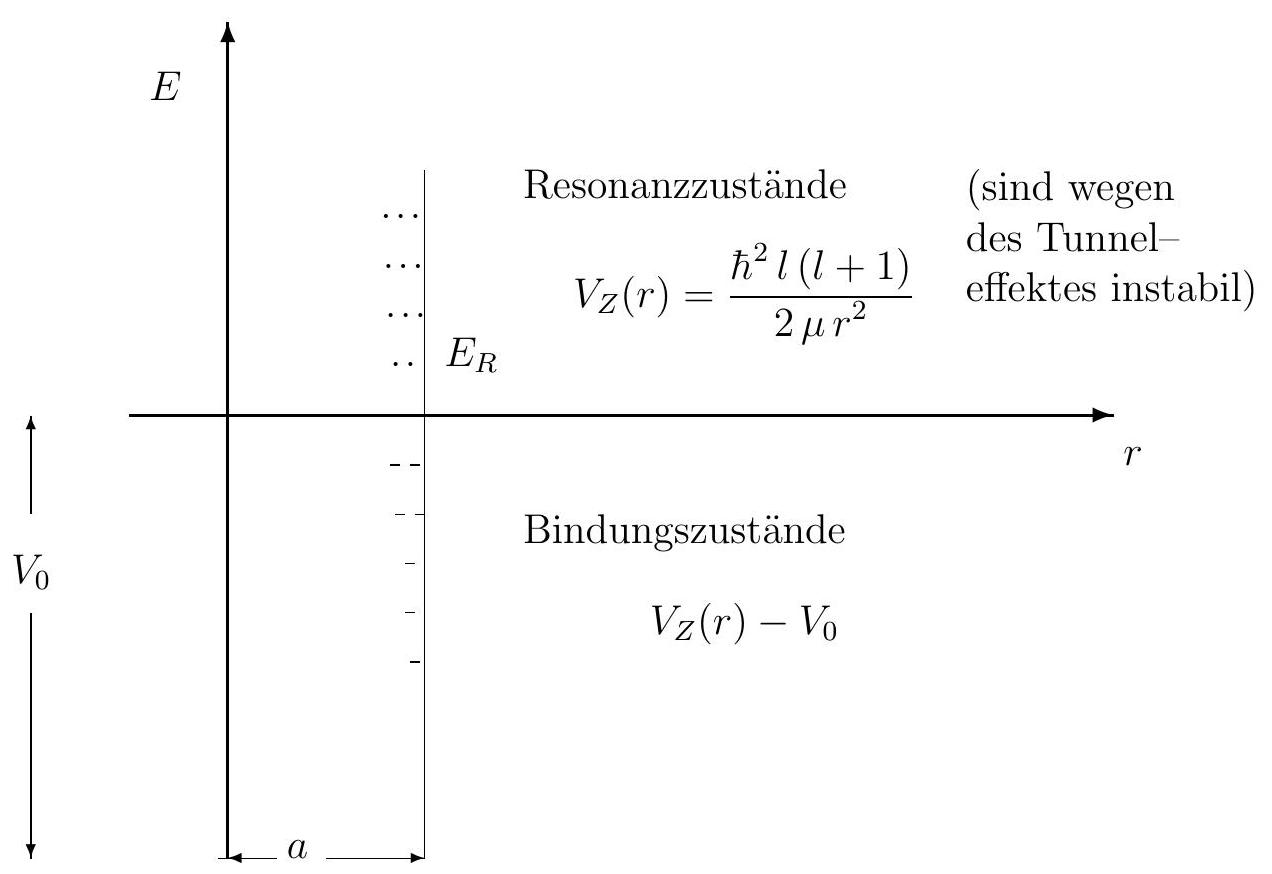
\includegraphics[scale=0.2, center]{2025_05_21_d5590f158a899e385c7cg-21}

\subsubsection*{Breit-Wigner Formel}
In der Nähe der Resonanz kann man näherungsweise

$$
\tan \delta_{l}=\gamma_{l} \frac{(k a)^{2 l+1}}{E-E_{R}}, \quad \gamma_{l}=\text { const }
$$

setzen: Schwellenverhalten für den Zähler, Taylor-Entwicklung um die Nullstelle im Nenner. Für den Wirkungsquerschnitt $\sigma_{l}$ der Partialwelle $l$ ergibt sich daraus

$$
\begin{aligned}
\sigma_{l}(E) & =\frac{4 \pi(2 l+1)}{k^{2}} \sin ^{2} \delta_{l}=\frac{4 \pi(2 l+1)}{k^{2}} \frac{\tan ^{2} \delta_{l}}{1+\tan ^{2} \delta_{l}} \\
& =\frac{4 \pi(2 l+1)}{k^{2}} \frac{\left(\gamma_{l}(k a)^{2 l+1}\right)^{2}}{\left(E-E_{R}\right)^{2}+\left(\gamma_{l}(k a)^{2 l+1}\right)^{2}}
\end{aligned}
$$

Dies ist die Breit-Wigner-Formel für den Wirkungsquerschnitt in der Umgebung der Resonanzenergie $E_{R}$.

\subsubsection*{Resonanzbreite}
Die entsprechende Amplitude der Partialwelle ist

$$
f_{l}(k)=\frac{1}{2 i k}\left(e^{2 i \delta_{l}(k)}-1\right)=\frac{1}{2 i k}\left(\frac{1+i \tan \delta_{l}}{1-i \tan \delta_{l}}-1\right)=\frac{1}{k} \frac{\tan \delta_{l}}{1-i \tan \delta_{l}}
$$

wobei wir $\exp (2 x)=\exp (x) / \exp (-x)$ verwendet haben. Man erhält

$$
f_{l}(k)=\frac{1}{k} \frac{\gamma_{l}(k a)^{2 l+1}}{E-E_{R}-i \gamma_{l}(k a)^{2 l+1}}
$$

Die Größe

$$
\Gamma_{l}=2 \gamma_{l}(k a)^{2 l+1}
$$

bezeichnet man als die Breite der Resonanz, da $\sigma_{l}\left(E_{R} \pm \frac{1}{2} \Gamma_{l}\right)=\frac{1}{2} \sigma_{l}\left(E_{R}\right)$.\\
Die Resonanzstreuung spielt eine zentral Rolle in der Atom-, Kern- und Elementarteilchenphysik. In ihrer allgemeinen Form gelten die hier hergeleiteten Formeln für viele Potentiale.\\
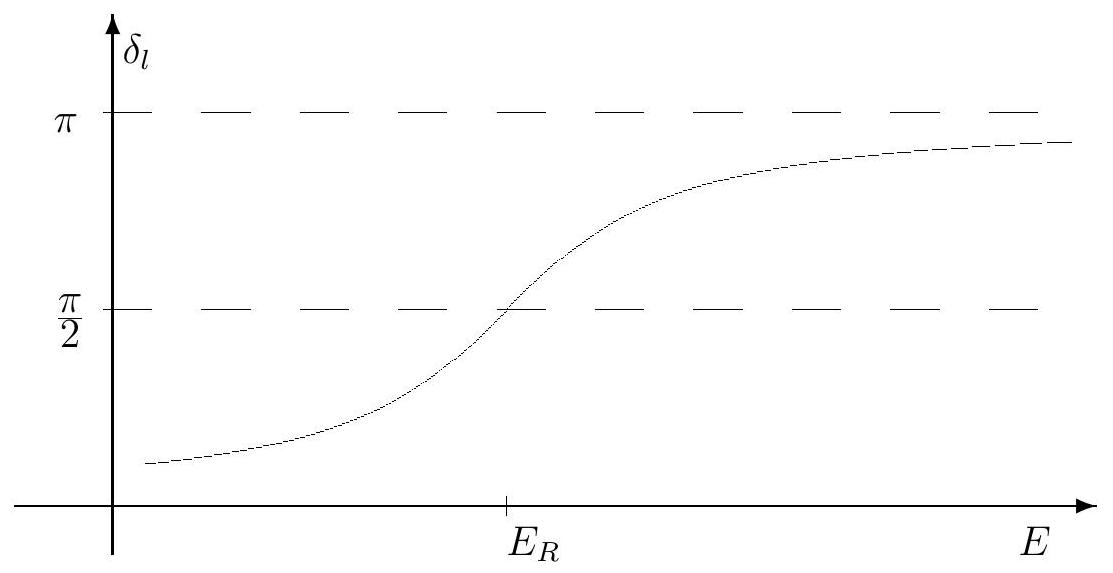
\includegraphics[scale=0.2, center]{2025_05_21_d5590f158a899e385c7cg-22}

















\pagebreak

\section{Der Spin der Elektronen}


---

\textbf{Spin als innerer Freiheitsgrad [Concept]}

Die Existenz des Spins bedeutet, dass Elektronen – zusätzlich zu Orts- und Impulskoordinate – einen weiteren Freiheitsgrad besitzen: Spin "oben" oder "unten", relativ zu einer gewählten Quantisierungsachse (z.B. \( x_3 \)-Achse), obwohl sie Punktteilchen sind.

---

\textbf{Definition des Spinors [Definition]}

Die gewöhnliche Wellenfunktion wird zu einem Spinor erweitert:

\[
\psi(\vec{x}, t) \rightarrow \tilde{\psi}(\vec{x}, t)=\begin{pmatrix}\psi_+(\vec{x}, t)\\ \psi_-(\vec{x}, t)\end{pmatrix}
\]

Dabei steht \( \psi_+ \) für Spin "oben", \( \psi_- \) für Spin "unten".

---

\textbf{Spinoperatoren durch Pauli-Matrizen [Definition]}

Die Spin-Operatoren sind gegeben durch:

\[
\vec{\mathbf{S}} = \frac{\hbar}{2} (\sigma_1, \sigma_2, \sigma_3)
\]

mit den Pauli-Matrizen:

\[
\sigma_1 = \begin{pmatrix}0 & 1 \\ 1 & 0\end{pmatrix},\quad
\sigma_2 = \begin{pmatrix}0 & -i \\ i & 0\end{pmatrix},\quad
\sigma_3 = \begin{pmatrix}1 & 0 \\ 0 & -1\end{pmatrix}
\]

Sie erfüllen:

\[
[\sigma_k, \sigma_l] = 2i \varepsilon_{klm} \sigma_m,\quad \sigma_j^2 = 1
\]

---

\textbf{Eigenbasis für \(\mathbf{S}_3\) [Definition]}

Die Eigenzustände für Spin "oben" und "unten" lauten:

\[
\tilde{\psi}_+ = \begin{pmatrix}1 \\ 0\end{pmatrix},\quad
\tilde{\psi}_- = \begin{pmatrix}0 \\ 1\end{pmatrix}
\]

mit:

\[
\mathbf{S}_3 \tilde{\psi}_+ = \frac{\hbar}{2} \tilde{\psi}_+,\quad
\mathbf{S}_3 \tilde{\psi}_- = -\frac{\hbar}{2} \tilde{\psi}_-
\]

---

\textbf{Allgemeine Spinoren und Normierung [Concept]}

Allgemeiner Spinor als Linearkombination:

\[
\tilde{\psi}(\vec{x}, t) = c_+(\vec{x}, t)\tilde{\psi}_+ + c_-(\vec{x}, t)\tilde{\psi}_- = \begin{pmatrix}c_+(\vec{x}, t)\\ c_-(\vec{x}, t)\end{pmatrix}
\]

Die Norm lautet:

\[
(\tilde{\psi}, \tilde{\psi}) = |c_+|^2 + |c_-|^2 = 1
\]

wobei \( |c_\pm|^2 \) die Wahrscheinlichkeit für Spin "oben"/"unten" angeben.

---

\textbf{Erwartungswerte der Spin-Komponenten [Proposition]}

Für konstanten Spinor (Ortsabhängigkeit ignoriert):

\[
\langle \mathbf{S}_1 \rangle = \frac{\hbar}{2}(c_+^*c_- + c_-^*c_+)
\]
\[
\langle \mathbf{S}_2 \rangle = -\frac{i\hbar}{2}(c_+^*c_- - c_-^*c_+)
\]
\[
\langle \mathbf{S}_3 \rangle = \frac{\hbar}{2}(|c_+|^2 - |c_-|^2)
\]

Alle Erwartungswerte sind reell.

---

\textbf{Drehung von Spinoren [Concept]}

Analog zur Drehung von Wellenfunktionen \( \psi(R\vec{x}) = e^{-i\vec{\mathbf{L}}\cdot \vec{\varphi}/\hbar} \psi(\vec{x}) \) gilt für Spin:

\[
R \tilde{\psi} = e^{-i\vec{\mathbf{S}}\cdot \vec{\varphi}/\hbar} \tilde{\psi}
\]

---

\textbf{Drehung um die z-Achse für Spin-\(\frac{1}{2}\) [Example]}

Für eine Rotation um die z-Achse mit \( \vec{\varphi} = (0,0,\varphi) \) ergibt sich:

\[
e^{-i \mathbf{S}_3 \varphi / \hbar}
= \cos (\varphi / 2)\mathbb{I}
- i \sin (\varphi / 2)\sigma_3
= \begin{pmatrix}
e^{-i\varphi/2} & 0 \\
0 & e^{i\varphi/2}
\end{pmatrix}
\]

Die beiden Spin-Komponenten erhalten entgegengesetzte Phasen.

\[
\text{Eine Drehung um } 2\pi \text{ bewirkt: } \tilde{\psi} \mapsto -\tilde{\psi}
\Rightarrow \text{erst bei } 4\pi \text{ ist } \tilde{\psi} \text{ wieder identisch.}
\]

---

\textbf{Magnetisches Moment eines Elektrons mit Spin [Concept]}

Ein Elektron mit Spin wirkt wie ein Ringstrom mit Drehimpuls \( \vec{S} \) und erzeugt ein magnetisches Moment:

\[
\vec{\mu} = -\frac{e_0 g}{2 m_e} \vec{S}, \quad \text{mit } g \approx 2
\]

Dabei ist \( g \) der gyromagnetische Faktor. Klassisch wäre \( g = 1 \).

---

\textbf{Hamiltonoperator für Spin im Magnetfeld [Definition]}

Ein magnetisches Moment \( \vec{\mu} \) im äußeren Feld \( \vec{B} \) trägt zur Energie bei durch:

\[
H = -\vec{\mu} \cdot \vec{B}
\Rightarrow
\mathbf{H} = \frac{e_0 g \hbar}{4 m_e} \vec{\sigma} \cdot \vec{B}
\]

---

\textbf{Schrödingergleichung für Spin-\(\frac{1}{2}\) im Magnetfeld [Proposition]}

Für einen zeitabhängigen Spinor

\[
\tilde{\psi}(t) = \begin{pmatrix}c_+(t) \\ c_-(t)\end{pmatrix}
\]

ergibt sich die Gleichung:

\[
i\hbar \frac{d}{dt} \tilde{\psi}(t) = \frac{e_0 g \hbar}{4 m_e} (\vec{\sigma} \cdot \vec{B}) \tilde{\psi}(t)
\]


---

\textbf{Larmor-Frequenz im Magnetfeld [Proposition]}

Für ein konstantes Magnetfeld \( \vec{B} = (0, 0, B_0) \) ergibt sich mittels Ansatz \( \tilde{\psi}(t) = e^{-i \omega t} \begin{pmatrix} c_+ \\ c_- \end{pmatrix} \), mit \( c_\pm = \text{const.} \), aus der Schrödingergleichung:

\[
\hbar \omega \begin{pmatrix} c_+ \\ c_- \end{pmatrix}
= \frac{e_0 g \hbar B_0}{4 m_e}
\begin{pmatrix} 1 & 0 \\ 0 & -1 \end{pmatrix}
\begin{pmatrix} c_+ \\ c_- \end{pmatrix}
\]

Die Eigenfrequenzen sind:

\[
\omega_{\pm} = \pm \omega_L = \pm \frac{e_0 g B_0}{4 m_e}
\]

und die zugehörigen Eigenvektoren \( (1,0) \) und \( (0,1) \) führen zum allgemeinen Zustand:

\[
\tilde{\psi}(t) = \begin{pmatrix} a e^{-i \omega_L t} \\ b e^{i \omega_L t} \end{pmatrix},
\quad |a|^2 + |b|^2 = 1
\]

---

\textbf{Spinpräzession im Magnetfeld [Example]}

Für Anfangszustand mit Spin entlang der 1-Achse (senkrecht zu \( \vec{B} \)):

\[
\mathbf{S}_1 \begin{pmatrix} a \\ b \end{pmatrix} = \frac{\hbar}{2} \begin{pmatrix} a \\ b \end{pmatrix}
\Rightarrow \begin{pmatrix} a \\ b \end{pmatrix} = \frac{1}{\sqrt{2}} \begin{pmatrix} 1 \\ 1 \end{pmatrix}
\]

Dann ergibt sich für die Erwartungswerte:

\[
\begin{aligned}
\langle \mathbf{S}_1 \rangle(t) &= \frac{\hbar}{2} \cos (2 \omega_L t) \\
\langle \mathbf{S}_2 \rangle(t) &= \frac{\hbar}{2} \sin (2 \omega_L t) \\
\langle \mathbf{S}_3 \rangle(t) &= 0
\end{aligned}
\]

Der Spin präzediert mit Frequenz \( 2\omega_L \) um \( \vec{B} \).

---

\textbf{Paramagnetische Resonanz und g-Faktor [Concept]}

Der gyromagnetische Faktor \( g \) in

\[
\vec{\mu} = \frac{q g}{2m} \vec{\mathbf{S}}, \quad \vec{\mathbf{S}} = \frac{\hbar}{2} \vec{\sigma}
\]

ist keine universelle Konstante, sondern hängt z.B. im Festkörper von der chemischen Umgebung ab. Seine Bestimmung erfolgt über die paramagnetische Resonanz.

---

\textbf{RF-Feld-Induktion zwischen Spin-Zuständen [Definition]}

Ein oszillierendes Magnetfeld im RF-Bereich

\[
\vec{B}(t) = \left( B \cos \omega t, B \sin \omega t, B_0 \right)
\]

bewirkt über

\[
\vec{\sigma} \cdot \vec{B}(t)
= \begin{pmatrix} B_0 & B e^{-i\omega t} \\ B e^{i\omega t} & -B_0 \end{pmatrix}
\]

eine zeitabhängige Hamiltonmatrix:

\[
i \hbar \frac{d \tilde{\psi}}{dt}
= \frac{\hbar q g}{4m}
\begin{pmatrix} B_0 & B e^{-i\omega t} \\ B e^{i\omega t} & -B_0 \end{pmatrix}
\tilde{\psi}(t)
\]

---

\textbf{Variation der Konstanten im RF-Feld [Concept]}

Mit Ansatz:

\[
\tilde{\psi}(t) =
\begin{pmatrix}
a(t) e^{-i\omega_L t} \\
b(t) e^{i\omega_L t}
\end{pmatrix}
\]

folgt:

\[
\begin{aligned}
\dot{a} &= -i \omega_g e^{i(2\omega_L - \omega)t} b(t) \\
\dot{b} &= -i \omega_g e^{-i(2\omega_L - \omega)t} a(t) \\
\omega_g &= \frac{g e_0 B}{4 m}
\end{aligned}
\]

Einsetzen ergibt die Differenzialgleichung zweiter Ordnung:

\[
\ddot{a} - i(2\omega_L - \omega)\dot{a} + \omega_g^2 a = 0
\]

---

\textbf{Lösungen und Übergangswahrscheinlichkeiten [Proposition]}

Lösungsansatz:

\[
a(t) = A e^{i\lambda t}
\Rightarrow
\lambda_{1,2} = \omega_L - \frac{\omega}{2} \pm \sqrt{\left(\omega_L - \frac{\omega}{2}\right)^2 + \omega_g^2}
\]

Für Startzustand \( a(0)=1, b(0)=0 \) ergibt sich:

\[
\begin{aligned}
a(t) &= \left[\cos(\widehat{\omega} t) - i \frac{\omega_L - \omega/2}{\widehat{\omega}} \sin(\widehat{\omega} t) \right]
e^{i(\omega_L - \omega/2)t} \\
b(t) &= -i \frac{\omega_g}{\widehat{\omega}} \sin(\widehat{\omega} t)
e^{-i(\omega_L - \omega/2)t} \\
\widehat{\omega} &= \sqrt{(\omega_L - \omega/2)^2 + \omega_g^2}
\end{aligned}
\]

Übergangswahrscheinlichkeit am Ende eines RF-Pulses der Dauer \( T \):

\[
|b(T)|^2 =
\frac{\omega_g^2}{(\omega_L - \omega/2)^2 + \omega_g^2}
\sin^2\left(T \sqrt{(\omega_L - \omega/2)^2 + \omega_g^2} \right)
\]

---

\textbf{Resonanzbedingung und $\pi$-Puls [Definition]}

Maximale Übergangsrate bei Resonanz:

\[
\omega = 2 \omega_L \Rightarrow |b(T)|^2 = 1
\]

Dies tritt bei Pulsdauer \( T = \frac{\pi}{2 \omega_g} \) ein („$\pi$-Puls“). Anwendung in Kernspinresonanz (NMR), Myonspinrotation ($\mu$SR), Medizin und Materialphysik.




\pagebreak


\subsection*{Quantenmechanische Beschreibung}
Die Existenz des Spins bedeutet, daß Elektronen, außer der Ortskoordinate $\vec{x}$, oder der Impulskoordinate $\vec{p}$, einen weiteren Freiheitsgrad besitzen: Spin nach "oben" und Spin nach "unten", jeweils bezüglich einer vorgegebenen Richtung (Quantisierungsachse, z.B. die $x_{3}$-Richtung). Und dieses obwohl Elektronen Punktteilchen sind.

\subsubsection*{Spinore}
Man verdoppelt die Wellenfunktion $\psi(\vec{x}, t)$ zu einem Spinor $\tilde{\psi}(\vec{x}, t)$,

$$
\psi(\vec{x}, t) \rightarrow \quad \tilde{\psi}(\vec{x}, t)=\binom{\psi_{+}(\vec{x}, t)}{\psi_{-}(\vec{x}, t)}
$$

wobei $\psi_{+}(\vec{x}, t)$ ein Elektron mit Spin "oben" und $\psi_{-}(\vec{x}, t)$ ein Elektron mit Spin "unten" beschreibt.

\subsubsection*{Pauli-Matrizen}
Der Spin-Operator $\overrightarrow{\mathbf{S}}$ ist nach Anbschnitt ?? durch die Pauli-Matrizen $\sigma_{i}$ gegeben,

$$
\begin{aligned}
\overrightarrow{\mathbf{S}} & =\frac{\hbar}{2}\left(\sigma_{1}, \sigma_{2}, \sigma_{3}\right) \\
\sigma_{1} & =\left(\begin{array}{cc}
0 & 1 \\
1 & 0
\end{array}\right), \quad \sigma_{2}=\left(\begin{array}{cc}
0 & -i \\
i & 0
\end{array}\right), \quad \sigma_{3}=\left(\begin{array}{cc}
1 & 0 \\
0 & -1
\end{array}\right)
\end{aligned}
$$

Bis auf den Faktor $\hbar / 2$ folgen die Pauli Matrizen den Kommuationsrelationen von Drehimpulsoperatoren,

$$
\left[\sigma_{k}, \sigma_{l}\right]=2 i \epsilon_{k l m} \sigma_{m}, \quad \sigma_{j}^{2}=1, \quad j=1,2,3
$$

\subsubsection*{Basiswahl}
Bezeichen wir mit $\tilde{\psi}_{ \pm}$die Zustände mit Spin rauf/runter,

$$
\tilde{\psi}_{+}=\binom{1}{0}, \quad \tilde{\psi}_{-}=\binom{0}{1}
$$

so gilt erwartungsgemäß:

$$
\mathbf{S}_{3} \tilde{\psi}_{+}=\frac{\hbar}{2}\left(\begin{array}{cc}
1 & 0 \\
0 & -1
\end{array}\right)\binom{1}{0}=\frac{\hbar}{2}\binom{1}{0}, \quad \mathbf{S}_{3} \tilde{\psi}_{-}=-\frac{\hbar}{2}\binom{0}{1}
$$

Für festes $\vec{x}$ und $t$ spannen $\tilde{\psi}_{+}$und $\tilde{\psi}_{-}$einen 2-dimionalen Vektorraum auf, dessen Elemente als Spinoren bezeichnet werden.

\subsubsection*{Wellenfunktionen}
Ein allgemeines Element des Vektorraums hat komplexen Koeffizienten $c_{+}$und $c_{-}$, die orts- und zeitabhängig sind:

$$
\tilde{\psi}(\vec{x}, t)=c_{+}(\vec{x}, t) \tilde{\psi}_{+}+c_{-}(\vec{x}, t) \tilde{\psi}_{-}=\binom{c_{+}(\vec{x}, t)}{c_{-}(\vec{x}, t)}
$$

Die Entwicklungskoeffizienten $c_{ \pm}(\vec{x}, t)$ entsprechen also Wellenfunktionen $\psi_{ \pm}(\vec{x}, t)$, von denen es pro Elektron nun zwei gibt. Die Norm von $\tilde{\psi}(\vec{x}, t)$ ist durch

$$
(\tilde{\psi}, \tilde{\psi})=\left|c_{+}\right|^{2}+\left|c_{-}\right|^{2}
$$

gegeben. Wegen der physikalischen Interpretation muss $(\tilde{\psi}, \tilde{\psi})=1$ sein. $\left|c_{ \pm}\right|^{2}$ ist damit die Wahrscheinlichkeit dafür, daß ein Elektron im Zustand $\psi$ den Spin parallel/antiparallel zur $x_{3}$-Achse ausgerichtet hat, mit $\left|c_{+}\right|^{2}+\left|c_{-}\right|^{2}=1$.

\subsubsection*{Erwartungswerte}
Im folgenden wird die Ortsabhängigkeit von $\tilde{\psi}$ ignoriert und zunächst nur Spineigenschaften betrachtet. Für die Erwartungswerte $\left\langle\mathbf{S}_{j}\right\rangle$ der Komponenten $\mathbf{S}_{j}$ im Zustand $\tilde{\psi}$ ergibt sich

$$
<\mathbf{S}_{1}>=\frac{\hbar}{2}\left(c_{+}^{*}, c_{-}^{*}\right)\left(\begin{array}{ll}
0 & 1 \\
1 & 0
\end{array}\right)\binom{c_{+}}{c_{-}}=\frac{\hbar}{2}\left(c_{+}^{*} c_{-}+c_{-}^{*} c_{+}\right),
$$

und analog

$$
\begin{aligned}
& <\mathbf{S}_{2}>=-\frac{i \hbar}{2}\left(c_{+}^{*} c_{-}-c_{-}^{*} c_{+}\right) \\
& <\mathbf{S}_{3}>=\frac{\hbar}{2}\left(\left|c_{+}\right|^{2}-\left|c_{-}\right|^{2}\right)
\end{aligned}
$$

Als Observable sind die Erwartungswerte reel.

\subsection*{Drehungen von Spins}
Im Abschnitt ?? wurde gezeigt, daß Wellenfunktionen via

$$
\psi(R \vec{x})=e^{-i \overrightarrow{\mathbf{L}} \cdot \vec{\varphi} / \hbar} \psi(\vec{x})
$$

gedreht werden. Dieses gilt für ganzzahligen Drehimpuls $j=0,1,2 \ldots$ Für $j=1 / 2$ ist der Drehimpulsoperatoren $\vec{L}$ durch den Spin-Operator $\vec{S}$ zu ersetzen,

$$
R \tilde{\psi}=e^{-i \overrightarrow{\mathbf{S}} \cdot \vec{\varphi} / \hbar} \tilde{\psi}
$$

wobei $\tilde{\psi}$ ein Spinor ist.

\subsubsection*{Drehung um die z-Achse}
Als Beispiel betrachten wir eine Drehung um die 3-Achse, d.h. $\vec{\varphi}=(0,0, \varphi)$ :

$$
\begin{aligned}
e^{-i \mathbf{S}_{3} \varphi / \hbar} & =\sum_{n=0}^{\infty} \frac{(-i \varphi / 2)^{n}}{n!}\left(\begin{array}{cc}
1 & 0 \\
0 & -1
\end{array}\right)^{n} \\
& =\sum_{l=0}^{\infty} \frac{(-i \varphi / 2)^{(2 l)}}{(2 l)!}\left(\begin{array}{ll}
1 & 0 \\
0 & 1
\end{array}\right)+\sum_{l=0}^{\infty} \frac{(-i \varphi / 2)^{(2 l+1)}}{(2 l+1)!}\left(\begin{array}{cc}
1 & 0 \\
0 & -1
\end{array}\right) \\
& =\cos (\varphi / 2)\left(\begin{array}{ll}
1 & 0 \\
0 & 1
\end{array}\right)-i \sin (\varphi / 2)\left(\begin{array}{cc}
1 & 0 \\
0 & -1
\end{array}\right)=\left(\begin{array}{cc}
e^{-i \varphi / 2} & 0 \\
0 & e^{i \varphi / 2}
\end{array}\right)
\end{aligned}
$$

Spin nach oben und unten erhalten also entgegengesetzte Phasen.

$$
\text { Bei einer Drehung um } 2 \pi \text { erhalten Spinoren die Phase }(-1) \text {. }
$$

Um einen Spin in den Ausgangszustand überzuführen bedarf es also einer Drehung um $4 \pi$.

\subsection*{Das magnetische Moment des Elektrons}
\subsubsection*{Gyromagnetischer Faktor}
Ein Elektron mit Spin ist ein rotierendes (geladenes) Teilchen. Aus der Elektrodynamik wissen wir, daß ein Ringstrom mit Drehimpuls $\vec{L}=\vec{S}$ ein magnetisches Moment der Grösse

$$
\begin{aligned}
\vec{\mu} & =-\frac{e_{0} g}{2 m_{e}} \overrightarrow{\mathbf{S}} & & \text { mit } \\
g & \approx 2 & & \text { (in guter Näherung) }
\end{aligned}
$$

erzeugt. Der $g$-Faktor heißt gyromagnetischer Faktor. Für klassische Ringströme gilt $g=1$, siehe auch Abschnitt ??.

\subsubsection*{Elektron im Magnetfeld}
In einem äußeren Feld $\vec{B}$ hat ein klassisches magnetisches Moment $\vec{\mu}$ die Energie $-\vec{\mu} \cdot \vec{B}$. Nach dem Korrespondenzprinzip führt dies zum Hamilton-Operator

$$
\mathbf{H}=\frac{e_{0} g \hbar}{4 m_{e}} \vec{\sigma} \cdot \vec{B}
$$

Für einen zeitabhängigen Spinor $\tilde{\psi}(t)=\binom{c_{+}(\vec{x}, t)}{c_{-}(\vec{x}, t)}$ erhalten wir die zeithabhängige Schrödinger-Gleichung

$$
i \hbar \frac{d}{d t} \tilde{\psi}(t)=\frac{e_{0} g \hbar}{4 m_{e}}(\vec{\sigma} \cdot \vec{B}) \tilde{\psi}(t)
$$

\subsubsection*{Lamor-Frequenz}
Wir betrachten ein konstantes Magnetfeld $\vec{B}=\left(0,0, B_{0}\right)$ und lösen die SchrödingerGleichung mittels des Ansatzes $\tilde{\psi}(t)=e^{-i \omega t}\binom{c_{+}}{c_{-}}$, mit $c_{ \pm}=$const., also

$$
\hbar \omega\binom{c_{+}}{c_{-}}=\frac{e g \hbar B_{0}}{4 m_{e}}\left(\begin{array}{cc}
1 & 0 \\
0 & -1
\end{array}\right)\binom{c_{+}}{c_{-}} .
$$

Die beiden Eigenfrequenzen $\omega_{ \pm}$sind

$$
\omega_{+}=\frac{e_{0} g B_{0}}{4 m_{e}} \equiv \omega_{L} \quad \text { und } \quad \omega_{-}=-\omega_{L}
$$

mit Eigenvektoren sind $(1,0)$ und $(0,1)$. Hier is $\omega_{L}$ die Lamor-Frequenz. ${ }^{1}$ Für einen allgemeinen Anfangszustand $\tilde{\psi}(t=0)=(a, b)$ findet man daher

$$
\tilde{\psi}(t)=\binom{a e^{-i \omega_{L} t}}{b e^{i \omega_{L} t}}, \quad \omega_{L}=\frac{e_{0} g B}{4 m_{e}}, \quad|a|^{2}+|b|^{2}=1
$$

\subsubsection*{Präzession}
Als Beispiel betrachten wir einen Anfangszustand, in welchem der Spin entlang der 1Achse ausgericht ist, also senkrecht zum angelegten Magnetfeld.

Als Erstes müssen wir den Eigenvektor $(a, b)$ zu $\mathbf{S}_{1}$ (und zum Eigenwert $\hbar / 2$ ) finden:

$$
\frac{1}{2} \hbar\left(\begin{array}{ll}
0 & 1 \\
1 & 0
\end{array}\right)\binom{a}{b}=\frac{1}{2} \hbar\binom{a}{b}, \quad\binom{a}{b}=\frac{1}{\sqrt{2}}\binom{1}{1} .
$$

\footnotetext{${ }^{1}$ Die hier definierte Larmor-Frequenze gilt für Spin-1/2. Klassisch benutzt man $q g B /(2 m)$. Unter Einberechnung der $g$-Faktoren erhält man sehr ähnliche Werte.
}Wir berechnen nun den Zeit-abhängigen Erwartungswert,

$$
\begin{aligned}
\left(\tilde{\psi}(t), \mathbf{S}_{1} \tilde{\psi}(t)\right) & =<\mathbf{S}_{1}>(t) \\
& =\frac{\hbar}{2} \frac{1}{\sqrt{2}}\left(e^{i \omega_{L} t}, e^{-i \omega_{L} t}\right)\left(\begin{array}{cc}
0 & 1 \\
1 & 0
\end{array}\right)\binom{e^{-i \omega_{L} t}}{e^{i \omega_{L} t}} \frac{1}{\sqrt{2}} \\
& =\frac{\hbar}{2} \cos 2 \omega_{L} t
\end{aligned}
$$

Analog ergibt sich

$$
\begin{aligned}
<\mathbf{S}_{1}>(t) & =\frac{\hbar}{2} \cos 2 \omega_{L} t \\
<\mathbf{S}_{2}>(t) & =\frac{\hbar}{2} \sin 2 \omega_{L} t \\
<\mathbf{S}_{3}>(t) & =0
\end{aligned}
$$

d.h. der Spin "präzediert" mit der doppelten Lamor-Frequenz um die Richtung von $\vec{B}$.

\subsection*{Paramagnetische Resonanz}
Der $g$-Faktor in der Beziehung

$$
\vec{\mu}=\frac{q g}{2 m} \overrightarrow{\mathbf{S}}, \quad \overrightarrow{\mathbf{S}}=\frac{1}{2} \hbar \vec{\sigma}, \quad q: \text { Ladung }
$$

ist im Festkörper keine universelle Konstante, sondern hängt von der chemischen Umgebung ab (via der Spin-Bahn Kopplung, siehe Abschnitt ??). Eine Methode die Größe des $g$-Faktors experimentell zu bestimmen ist die paramagnetische Resonanz.

\subsubsection*{RF-Felder}
Analog zu der Induktion von atomaren Übergängen zwischen verschiedenen Niveaus durch Einstrahlen von Licht, kann man Übergänge zwischen den beiden Energieniveaus $\pm \hbar \omega_{L}=$ $\hbar g|q| B_{0} /(4 m)$ eines Spins in einem konstanten Magnetfeld $B_{0}$ induzieren. Dafür benötigt man ein zusätzlich oszillierendes Magnetfeld $B$, typischerweise im Radiofrequenz (RF) Bereich.

Es sei also

$$
\vec{B}=\left(B \cos \omega t, B \sin \omega t, B_{0}\right)
$$

Mit

$$
\vec{\sigma} \cdot \vec{B}=\left(\begin{array}{cc}
B_{0}, & B(\cos \omega t-i \sin \omega t) \\
B(\cos \omega t+i \sin \omega t), & -B_{0}
\end{array}\right)
$$

lautet die Schrödinger-Gleichung (mit $q=-e_{0}$ )

$$
i \hbar \frac{d \tilde{\psi}}{d t}=\frac{\hbar q g}{4 m}\left(\begin{array}{cc}
B_{0}, & B e^{-i \omega t} \\
B e^{i \omega t}, & -B_{0}
\end{array}\right) \tilde{\psi}(t)
$$

\subsubsection*{Variation der Konstanten}
Die Energie ist nicht erhalten, da $\mathbf{H}=\mathbf{H}(t)=\hbar \omega_{g} \vec{\sigma} \cdot \vec{B}(t)$ explizit von der Zeit abhängt, analog zu erzwungenen Schwingungen in der Mechanik.

Der Ansatz (Variation der Konstanten)

$$
\tilde{\psi}(t)=\binom{a(t) e^{-i \omega_{L} t}}{b(t) e^{i \omega_{L} t}}, \quad \frac{d \tilde{\psi}}{d t}=\binom{\left(\dot{a}-i \omega_{L} a\right) e^{-i \omega_{L} t}}{\left(\dot{b}+i \omega_{L} b\right) e^{i \omega_{L} t}}
$$

führt zu den Gleichungen

$$
\begin{aligned}
\dot{a} & =-i \omega_{g} e^{i\left(2 \omega_{L}-\omega\right) t} b(t) \\
\dot{b} & =-i \omega_{g} e^{-i\left(2 \omega_{L}-\omega\right) t} a(t) \\
\omega_{g} & =\left(g e_{0} B\right) /(4 m)
\end{aligned}
$$

Differenzieren der 1. Gleichung nach $t$ und Einsetzen der zweiten ergibt

$$
\ddot{a}-i\left(2 \omega_{L}-\omega\right) \dot{a}+\omega_{g}^{2} a=0
$$

Der Ansatz $a(t)=A e^{i \lambda t}$ führt zu einer quadratischen Gleichung für $\lambda$, mit den Lösungen

$$
\lambda_{1,2}=\omega_{L}-\frac{1}{2} \omega \pm \sqrt{\left(\omega_{L}-\frac{1}{2} \omega\right)^{2}+\omega_{g}^{2}}
$$

Die Bewegung des Systems, d.h. des Spinors $\tilde{\psi}(t)$ wird also durch die äussere Frequenz $\omega$ moduliert.

\subsubsection*{Induzierte Übergänge}
Wir preparieren das System zur Zeit $t=0$ in den Spin-oben Zustand: $a(0)=1$ und $b(0)=0$, was auch $\dot{a}(0)=0$ bedeutet. Für allg. Zeiten gilt

$$
\begin{aligned}
a(t) & =\left[\cos (\widehat{\omega} t)-i \frac{\omega_{L}-\omega / 2}{\widehat{\omega}} \sin \widehat{\omega} t\right] e^{i\left(\omega_{L}-\omega / 2\right) t} \\
b(t) & =-i \frac{\omega_{g}}{\widehat{\omega}} \sin \widehat{\omega} t e^{-i\left(\omega_{L}-\omega / 2\right) t} \\
\widehat{\omega} & =\sqrt{\left(\omega_{L}-\frac{1}{2} \omega\right)^{2}+\omega_{g}^{2}}
\end{aligned}
$$

Ist $T$ die Zeitspanne, während der das RF-Magnetfeld eingeschaltet ist, so ist am Ende dieser Zeitspanne der Bruchteil $|b(T)|^{2}$ der Spins "umgeklappt":

$$
|b(T)|^{2}=\frac{\omega_{g}^{2}}{\left(\omega_{L}-\frac{\omega}{2}\right)^{2}+\omega_{g}^{2}} \sin ^{2}\left(T \sqrt{\left(\omega_{L}-\frac{\omega}{2}\right)^{2}+\omega_{g}^{2}}\right)
$$

man hat mittels des RF-Feldes Übergänge zwischen den beiden Zeeman-Niveaus $\pm \omega_{L}$ erzeugt.

\subsubsection*{Resonanz}
Resonanz liegt vor, falls die Frequenz des RF-Feldes $\omega=2 \omega_{L}$ ist, also genau der Energiedifferenz der beiden Energieniveaus entspricht. Bei Resonanz ist es möglich, alle Spins umzudrehen, $|b(T)|=1$. Man wähle hierfür eine Einschaltzeit $T=\pi /\left(2 \omega_{g}\right)$, da dann $\sin ^{2}=1$ ( $\pi$-Puls).

Die obige "paramagnetische" Resonanzmethode hat viele Anwendungen in der Atomund Kernphysik, der Festkörperphsik (NMR, $\mu$ SR) sowie auch in der Medizin.



\pagebreak

\section{Zur Struktur der Quantenmechanik}

\subsection*{Der quantenmechanische Hilbert-Raum}

\subsubsection*{Linearer Zustandsraum}
Die quantenmechanischen Zustände bilden einen linearen Raum. Beispiel sind die bisher diskutierten 1-Teilchen Zustände $\psi(\vec{x}, t)$.

\begin{itemize}
  \item Superpositionsprinzip
\end{itemize}

Sind $\psi_{1}$ und $\psi_{2}$ physikalisch realisierbare Zustände, so ist es auch

$$
\lambda_{1} \psi_{1}+\lambda_{2} \psi_{2}, \quad \lambda_{1}, \lambda_{2} \in \mathcal{C}
$$

\begin{itemize}
  \item Elementarteilchen
\end{itemize}

Das Superpositionsprinzip gilt für identische Elementarteilchen. Als solche lassen sich z.B. Elektronen und Neutronen nicht überlagern

\begin{itemize}
  \item Produktraum
\end{itemize}

Die Wellenfunktion des Wasserstoffatoms ist durch das Produkt $\psi=\psi_{p} \cdot \psi_{e}$ der Proton-Wellenfunkton $\psi_{p}$, und der des Elektrons, $\psi_{e}$, gegeben. Für Produktzustände gilt wiederum das Superpositionsprinzip.

\begin{itemize}
  \item Vielteilchenzustände
\end{itemize}

Es gibt mehr als nur ein Elektron in der Welt. Die entsprechenden Vielteilchenzustände haben wohl definierte Symmetrien, das ist u.A. der Stoff der Quanten-mechanik-2 (Spin-Statistik Theorem). Vielteilchenzustände bilden ebenfalls einen linearen Raum.

\subsubsection*{Skalarprodukt}
Im Raum der Zustände ist durch

$$
\left(\psi_{2}, \psi_{1}\right)=\int d x^{3} \psi_{2}^{*}(\vec{x}, t) \psi_{1}(\vec{x}, t), \quad(\psi, \psi)>0
$$

ein Skalarprodukt definiert. Es ist

\begin{itemize}
  \item antilinear im ersten Argument $\left(\lambda \psi_{1}, \psi_{2}\right)=\lambda^{*}\left(\psi_{1}, \psi_{2}\right)$,
  \item linear im zweiten Argument, $\left(\psi_{1}, \lambda \psi_{2}\right)=\lambda\left(\psi_{1}, \psi_{2}\right)$
  \item hermitisch $\left(\psi_{2}, \psi_{1}\right)=\left(\psi_{1}, \psi_{2}\right)^{*}$
  \item positiv definit $(\psi, \psi) \geq 0$\\
mit $\quad(\psi, \psi)=0 \quad \Leftrightarrow \quad \psi=0$.
\end{itemize}

\subsubsection*{Norm}
Mathematisch wird der Raum der Zustände durch das Skalarprodukt ( $\psi_{1}, \psi_{2}$ ) zu einem normierten Raum, mit der Definition der

\begin{itemize}
  \item Norm: $\|\psi\| \equiv+\sqrt{(\psi, \psi)}$
\end{itemize}

Meistens schreiben wir für die Norm $\|\psi\|$ von $\psi$ auch einfach $|\psi|$.

\subsubsection*{Konvergenz von Folgen}
Euklidischen kann man mittels der Norm die Konvergenz einer Folge $\left\{\psi_{n}, n=1, \ldots\right\}$ definieren:

$$
\left\{\psi_{n}, n=1, \ldots\right\} \quad \text { konvergent gegen } \psi, \text { falls } \quad \lim _{n \rightarrow \infty}\left\|\psi_{n}-\psi\right\|=0
$$

\subsubsection*{Cauchy Folgen}
Die Folge $\left\{\psi_{n}, n=1, \ldots\right\}$ heißt Cauchy-Folge, falls für beliebiges $\epsilon>0$ ein $N(\epsilon)$ existiert, so daß

$$
\left\|\psi_{n_{1}}-\psi_{n_{2}}\right\|<\epsilon, \quad \text { für } \quad n_{1}, n_{2}>N(\epsilon) .
$$

\subsubsection*{Vollständige Räume}
Falls zu jeder Cauchy-Folge im Raum ein Grenzelement gehört (wie im $\mathbb{R}^{n}$ ), so heißt der Raum vollständig.

Der Raum der stetigen Funktionen ist nicht vollständig. Jedoch kann man zeigen (Riesz-Fischer), daß der Raum der quadratintegrablen Funktionen vollständig ist. Physikalische Räume müssen vollständig sein.

\subsubsection*{Hilbert-Raum}
Ein vollständiger Vektorraum mit Skalarprodukt heißt Hilbert-Raum $\mathcal{H}$.

\subsubsection*{Dichte Untermengen}
Eine Untermenge des Hilbert-Raumes heißt dicht in $\mathcal{H}$, falls die Menge aller Grenzelemente $\mathcal{H}$ selbst ist.

\subsubsection*{Separable Hilbert-Räume}
Gibt es abzählbare Untermengen, die dicht sind, so heißt $\mathcal{H}$ separabel.

\begin{displayquote}
Quantenmechanische Hilberträume sind separabel.
\end{displayquote}

In der Praxis bedeutete das, dass es eine abzählbare Basis gibt.

\subsubsection*{Operatoren}
\subsubsection*{Selbstadjungierte Operatoren}
Ein selbstadjungierter Operator

$$
\mathbf{a}^{\dagger}=\mathbf{a}, \quad\left(\mathbf{a}^{\dagger} \psi_{1}, \psi_{2}\right)=\left(\psi_{1}, \mathbf{a} \psi_{2}\right), \quad \forall \psi_{1}, \psi_{2} \in \mathcal{H}
$$

hat reelle Eigenwerte.

\subsubsection*{Postulat}
Physikalischen Größen wie Ort, Impuls, Drehimpuls, Energie, etc. entsprechen selbstadjungierte Operatoren im Hilbertraum. Die Eigenwerte der der Operatoren bilden das "Spektrum" der möglichen Meßwerte.

\subsubsection*{Diskrete Spektren}
Bei endlich-dimensionalen Matrizen (wie z.B. beim Drehimpuls) ist das Spektrum "diskret", d.h. es gibt nur endlich viele verschiedene Eigenwerte und die zugehörigen Eigenvektoren liegen im Hilbertraum.

\subsubsection*{Kontinuierliche Spektren}
Bei Operatoren mit kontinuierlichem Spektrum sind die Eigenfunktionen nicht quadratintegrable, im eigentlichen Sinne bilden diese daher keinen Hilbertraum.

\begin{itemize}
  \item Ein Beispiel ist der Impuls-Operator,
\end{itemize}

$$
\mathbf{P}_{j}=\frac{\hbar}{i} \frac{d}{d x_{j}}, \quad j=1,2,3, \quad \quad e_{p}(\vec{x})=\frac{e^{i \vec{p} \cdot \vec{x} / \hbar}}{\sqrt{2 \pi \hbar}^{3}}
$$

\begin{itemize}
  \item Mathematisch läss sich das Problem der nicht-Integrabilät mittels einer GrenzwertBetrachtung lösen. Man betrachtet zuerst ein endlichen Volumen $V$, mit integrablen Eigenfunktionen
\end{itemize}

$$
e_{p}(\vec{x})=\frac{e^{i \vec{p} \cdot \vec{x} / \hbar}}{\sqrt{V}}
$$

und lässt das Volumen dann via $V \rightarrow \infty$ nach unendlich gehen.

\begin{itemize}
  \item Ein begrenztes physikalisches Volumen ist zu einem unendlich tiefen Potentialtopf äquivalent. Das hat eine abzählbare Basis zur Folge, wie wir in Abschnitt ?? gesehen haben.
\end{itemize}

Der Grenzübergang $V \rightarrow \infty$ wird z.B. in der Festkörperphysik eingehend diskutiert.

\subsubsection*{Nicht-entartete Eigenfunktionen}
In der Quantenmechanik benutzt man im Allgemeinen nicht eine beliebige orthogonale Basis, sondern eine welche der physikalischen Problemstellung angepasst ist, also den relevanten Observablen. D.h. man betrachtet einen selbstadjungierten Operator A, mit

$$
\mathbf{A} u_{j}=a_{j} u_{j}, \quad a_{j} \in \mathbb{R}
$$

Sind die Eigenwerte nicht entartet, d.h. gehört zu jedem $a_{j}, j_{1}=1,2, \ldots$, genau ein eindimensionaler Eigenvektorraum mit Eigenfunktion $u_{j}$. Die Eigenfunktionen $u_{j}$ bilden daher eine i.A. gut brauchbare orthogonale Basis,

\subsubsection*{Entartete Eigenfunktionen}
In der Regel werden die Eigenwerte eines Operators A jedoch entartet sein. Dann sucht man einen zweiten, physikalisch relevanten, Operator B, der mit A kommutiert,

$$
\mathrm{AB}=\mathrm{BA}
$$

Man kann dann die Eigenvektoren von B so wählen, daß diese gleichzeitig Eigenvektoren von A sind,

$$
\mathbf{B} u_{j l}=b_{j l} u_{j, l}, \quad \text { mit } \quad \mathbf{A} u_{j, l}=a_{j} u_{j, l}, \quad \forall l
$$

Im Allgemeinen werden zu einem Eigenwert $a_{j}$ von $\mathbf{A}$ verschiedene $b_{j l}$ gehören, mit Eigenvektoren $u_{j, l}$, d.h. die ursprüngliche Entartung wird reduziert.

\subsubsection*{Vollständiger Satz von kommutierenden Observablen}
Man setzt das Verfahren so lang fort, bis man einen Satz (A,B, C, . . ) von selbstadjungierten Operatoren mit folgenden Eigenschaften hat:

\begin{itemize}
  \item Je zwei der selbstadjungierten Operatoren kommutieren miteinander.
  \item Alle diese selbstadjungierten Operatoren haben gemeinsamen Eigenvektoren $u_{j, l, \ldots}$.
  \item Jeder Eigenvektor $u_{j, l, k, \ldots}$ ist einendeutig durch den Satz $\left(a_{j}, b_{j l}, c_{j l k}, \ldots\right)$ von Eigenwerten bestimmt.
  \item Verschiedene $u_{j, l, \ldots}$ sind zueinander orthogonal und bilden ein vollständiges System, d.h. jedes $\psi \in \mathcal{H}$ läßt sich nach den $u_{\alpha}$ entwickeln:
\end{itemize}

$$
\psi=\sum_{\alpha} c_{\alpha} u_{\alpha}, \quad c_{\alpha}=\left(u_{\alpha}, \psi\right), \quad \alpha=(j, l, \ldots)
$$

wobei $\alpha$ ein Multi-Index ist.\\
Man nennt die $\{\mathbf{A}, \mathbf{B}, \ldots\}$ einen vollständigen Satz von kommutierenden Observablen. Für das Wasserstoff-Atom ist

$$
\mathbf{A}=\mathbf{H}, \quad \mathbf{C}=\overrightarrow{\mathbf{L}}^{2}, \quad \mathbf{D}=\mathbf{L}_{3}, \quad \mathbf{E}=\mathbf{S}_{3}
$$

vollständigen Satz kommutierender Variablen.

\subsubsection*{Unterräume}
Sei $M \subset \mathcal{H}$ ein Unterraum des Hilbertraumes $\mathcal{H}$ und $M_{\perp}$ das orthogonale Komplement von $M$,

$$
\left(\psi_{M}, \psi_{M_{\perp}}\right)=0, \quad \forall \psi_{M} \in M, \quad \forall \psi_{M_{\perp}} \in M_{\perp}
$$

Wie $M$ ist auch $M_{\perp}$ ein Unterraum von $\mathcal{H}$, d.h. ein separabler Hilbertraum, d.h. abgeschlossen und vollständig.

Jeder Vektor $\psi \in \mathcal{H}$ läßt sich eindeutig in zwei Komponenten $\psi_{M}$ und $\psi_{M_{\perp}}$ zerlegen:

$$
\psi=\psi_{M}+\psi_{M_{\perp}}, \quad \psi_{M} \in M, \quad \psi_{M_{\perp}} \in M_{\perp}
$$

\subsubsection*{Projektionsoperatoren}
Der Projektionsoperator $\mathbf{P}_{M}$ auf den Unterraum $M$ wird via

$$
\mathbf{P}_{M} \psi=\psi_{M} \quad \forall \psi \in \mathcal{H}
$$

definiert. Somit gilt

$$
\mathbf{P}^{2} \psi=\mathbf{P} \mathbf{P} \psi=\mathbf{P} \psi_{M}=\psi_{M}, \quad \mathbf{P} \psi_{M_{\perp}}=0
$$

Umgekehrt projiziert $\mathbf{1 -} \mathbf{P}_{M}$ auf $M_{\perp}$. Projektionsoperatoren $\mathbf{P}$ haben folgende Eigenschaften:

\begin{itemize}
  \item Idempotent $\mathbf{P}^{2}=\mathbf{P}$
  \item Selbstadjungiert $\quad \mathbf{P}^{\dagger}=\mathbf{P}$
\end{itemize}

Seien $\psi_{1}, \psi_{2}$ beliebig, dann gilt

$$
\left(\psi_{2}, \mathbf{P}_{M} \psi_{1}\right)=\left(\psi_{2 M}+\psi_{2 M_{\perp}}, \psi_{1 M}\right)=\left(\psi_{2 M}, \psi_{1 M}\right)=\left(\mathbf{P}_{M} \psi_{2}, \psi_{1}\right)
$$

\begin{itemize}
  \item Die Eigenwerte sind 1 und 0
\end{itemize}

Sei $\mathbf{P} \psi=\lambda \psi$, dann ist

$$
\mathbf{P}^{2} \psi=\lambda^{2} \psi=\mathbf{P} \psi=\lambda \psi, \quad \lambda^{2}=\lambda, \quad \lambda=1,0,
$$

da $\mathbf{P}^{2}=\mathbf{P}$. Die Eigenvektoren zu $\lambda=1$ sind die Elemente von $M$, die zu $\lambda=0$ die in $M_{\perp}$.

\begin{itemize}
  \item Kommutationsregeln
\end{itemize}

Zwei Projektionsoperatoren auf die Unterräume $M_{1}$ und $M_{2}, \mathbf{P}_{1}$ und $\mathbf{P}_{2}$, kommutieren i.A. nicht. Falls $M_{1}$ orthogonal zu $M_{2}$ ist, dann hat man jedoch

$$
\mathbf{P}_{1} \mathbf{P}_{2}=\mathbf{P}_{2} \mathbf{P}_{1}=0
$$

\subsubsection*{Innere- und äußere Produkte}
Als Beispiel betrachten wir mit $\mathcal{H}$ einen n-dimensionaler Vektorraum. $A$ sei eine hermitesche Matrix mit nicht entarteten Eigenwerten $a_{j}$ und Eigenvektoren

$$
u_{j}=\left(\begin{array}{c}
c_{1}(j) \\
\vdots \\
c_{n}(j)
\end{array}\right) \quad \quad c_{i}(j) \text { komplex }
$$

Nach Vorraussetzung gilt

$$
u_{j}^{+} u_{k}=\left(c_{1}^{*}(j), \ldots c_{n}^{*}(j)\right)\left(\begin{array}{c}
c_{1}(k) \\
\vdots \\
c_{n}(k)
\end{array}\right)=\sum_{i} c_{i}^{*}(j) c_{i}(k)=\delta_{j k}
$$

für die entsprechenden Skalarprodukte. Das Skalarprodukt wird auch "inneres Produkt" genannt. Dem gegenüber entsprechen Projektionsoperatoren einem "äußerem Produkt",

$$
\begin{aligned}
\underset{\text { (keine Summation über } j \text { ) }}{\mathbf{P}_{j}=u_{j} u_{j}^{+}} & =\left(\begin{array}{c}
c_{1}(j) \\
\vdots \\
c_{n}(j)
\end{array}\right)\left(c_{1}^{*}(j), \ldots c_{n}^{*}(j)\right) \\
& \equiv\left(\begin{array}{ccc}
c_{1}(j) c_{1}^{*}(j) & \cdots & c_{1}(j) c_{n}^{*}(j) \\
\vdots & & \vdots \\
c_{n}(j) c_{1}^{*}(j) & \cdots & c_{n}(j) c_{n}^{*}(j)
\end{array}\right)
\end{aligned}
$$

Man verifiziert

$$
\mathbf{P}_{j} u_{k}=\left(u_{j} u_{j}^{+}\right) u_{k}=u_{j}\left(u_{j}^{+} u_{k}\right)=\delta_{j k} u_{j}
$$

sowie

$$
\begin{aligned}
\mathbf{P}_{j} \mathbf{P}_{k} & =u_{j} u_{j}^{+} \cdot u_{k} u_{k}^{+}=u_{k} \delta_{j k} u_{k}^{+}=\delta_{j k} u_{j} u_{j}^{+} \\
& =\delta_{j k} \mathbf{P}_{j}
\end{aligned}
$$

Die allgemeinen Schreibweisen für das innere-/äußere Produkt zwischen zwei Vektoren $\mathbf{a} / \mathbf{b}$ sind

$$
\begin{array}{|ll|}
\hline \mathbf{a} \cdot \mathbf{b}=\mathbf{a}^{\dagger} \mathbf{b} & \mathbf{a} \otimes \mathbf{b}=\mathbf{a} \mathbf{b}^{\dagger} \\
\hline
\end{array}
$$

Das Ergebnis des inneren-/äußeren Produkts ist ein Skalar/Matrix.

\subsubsection*{Entartete Eigenräume}
Ist $a_{j}$ entartet, mit zugehörigen orthonormalen Eigenvektoren $u_{j, s}$, wobie $s=1, \ldots, m_{j}$, dann lautet der Projektionsoperator auf den Eigenvektorraum

$$
\mathbf{P}_{j}=\sum_{s=1}^{m_{j}} u_{j s} \otimes u_{j s}
$$

\subsubsection*{Spektraldarstellung}
Sei A ein selbstadjungierter Operator mit den Eigenwerten $a_{j}$, möglicherweise entartet, und zugehörigen Eigenvektoren $u_{j}$, die einen Unterraum $M_{j}$ aufspannen. Weiterhin seien $\mathbf{P}_{j}$ die Projektionsoperatoren auf die Unterräume $M_{j}$, mit

$$
\mathbf{P}_{j} \mathbf{P}_{k}=\mathbf{P}_{k} \mathbf{P}_{j}=\delta_{j k} \mathbf{P}_{j} \quad \sum \mathbf{P}_{j}=\mathbf{1}
$$

Man nennt dann

$$
\mathbf{A}=\sum_{j} a_{j} \mathbf{P}_{j}
$$

$$
\mathbf{A} u_{j}=a_{j} u_{j}
$$

die Spektraldarstellung von A.

\subsubsection*{Operatorfunktionen}
In seiner Spektraldarstellung ist ein Operator diagonal. Daher kann man Funktionen eines Operators A via

$$
f(\mathbf{A})=\sum_{j} f\left(a_{j}\right) \mathbf{P}_{j}
$$

definieren.

\subsubsection*{Dirac Notation}
Die Spektraldarstellung

$$
\begin{aligned}
\mathbf{A} u_{j} & =a_{j} u_{j} & u_{j}^{+} u_{k} & =\delta_{j k} \\
\mathbf{A} & =\sum a_{j} \mathbf{P}_{j} & \sum \mathbf{P}_{j} & =\mathbf{1}
\end{aligned} \quad u_{j} u_{j}^{+}=\mathbf{P}_{j}
$$

gilt für alle selbstadjungierten Operatoren, auch für solche mit kontinuierlichem Spektrum.\\
Dirac hat in diesem Zusammenhang eine formale Schreibweise entwickelt, die diesem nicht-trivialen Sachverhalt Rechnung trägt:

$$
\begin{aligned}
u_{j} & \equiv\left|a_{j}\right\rangle & u_{j}^{+} & \equiv\left\langle a_{j}\right| \\
u_{j}^{+} u_{k} & \equiv\left\langle a_{j} \mid a_{k}\right\rangle & u_{j} u_{j}^{+} & =\left|a_{j}\right\rangle\left\langle a_{j}\right| \\
\mathbf{A} & =\sum_{j} a_{j}\left|a_{j}\right\rangle\left\langle a_{j}\right| & \sum_{j}\left|a_{j}\right\rangle\left\langle a_{j}\right| & =\mathbf{1} \\
(\psi, \mathbf{A} \psi) & =\langle\psi| \mathbf{A}|\psi\rangle & &
\end{aligned}
$$

Man bezeichnet mit

\begin{itemize}
  \item $\langle a|$ ("bra") den zu
  \item $|a\rangle$ ("ket") dualen Vektor und
  \item $\left\langle a_{j} \mid a_{j}\right\rangle$ als "bracket".
\end{itemize}

Wichtig ist:

$$
\text { Der Zustand }|a\rangle \text { ist Basis-unabhängig. }
$$

\subsubsection*{Darstellung der Identität}
Die Summe der Projektionsoperatoren über eine vollständige Basis ist die Einheitsmatrix,

$$
\sum_{j}\left|a_{j}\right\rangle\left\langle a_{j}\right|=1=\int_{a}|a\rangle\langle a|,
$$

welche sowohl für discrete wie für kontinuierliche Spektren gilt (oder für kombinierte).

\subsubsection*{Spektraldarstellung}
Die Orthonormierung für diskrete und kontinuierliche Eigenwerte $a_{j}$ und $a$ schreibt sich als

$$
\left\langle a_{i} \mid a_{j}\right\rangle=\delta_{i, j}, \quad\left\langle a^{\prime} \mid a\right\rangle=\delta\left(a^{\prime}-a\right)
$$

Ein selbstadjungierter Opertor $\mathbf{A}$ kann sowohl ein kontinuierliches wie ein diskretes Spektrum haben, mit der Spektraldarstellung

$$
\mathbf{A}=\underbrace{\int d a a|a\rangle\langle a|}_{\text {kontinuierliches Spektrum }}+\underbrace{\sum_{j} a_{j}\left|a_{j}\right\rangle\left\langle a_{j}\right|}_{\text {diskretes Spektrum }}
$$

Für das Wasserstoffatom sind die gebundenen Zustände mit $E<0$ Teil des diskreten Spektrums, die Streuzustände mit $E \geq 0$ bilden das kontinuierliche Spektrum.

\subsubsection*{Ortsdarstellung}
Wir betrachten den Ortsoperator Q, hier der Einfachheit halber in einer Dimension:

$$
\begin{aligned}
\mathbf{Q}|x\rangle & =x|x\rangle \quad \mathbf{Q}=\int_{-\infty}^{+\infty} d x x|x\rangle\langle x| \\
\left\langle x^{\prime} \mid x\right\rangle & =\delta\left(x^{\prime}-x\right) \\
\left\langle x^{\prime}\right| \mathbf{Q}|x\rangle & =x \delta\left(x^{\prime}-x\right)
\end{aligned}
$$

Die Entwicklung eines Zustandes $|\psi\rangle$ nach den Eigenzuständen des Ortsoperators ist dementsprechend

$$
\begin{aligned}
|\psi\rangle & =\int d x \psi(x)|x\rangle \\
\left\langle x^{\prime} \mid \psi\right\rangle & =\int d x \psi(x)\left\langle x^{\prime} \mid x\right\rangle=\psi\left(x^{\prime}\right)
\end{aligned}
$$

Die Wellenfunktion $\psi(x)=\langle x \mid \psi\rangle$ entspricht also der Orts-Darstellung von $\psi$. Man spricht auch von der Schrödinger-Darstellung des Zustandes $|\psi\rangle$.

\subsubsection*{Impulsdarstellung}
Für jeden Zustand $|p\rangle$ gilt

$$
|p\rangle=\left(\int d x^{\prime}\left|x^{\prime}\right\rangle\left\langle x^{\prime}\right|\right)|p\rangle=\int d x^{\prime}\left\langle x^{\prime} \mid p\right\rangle\left|x^{\prime}\right\rangle
$$

Sei nun $|p\rangle$ Eigenvektor des Impulsopertators P. Es gilt

$$
\langle x| P|p\rangle=p\langle x \mid p\rangle, \quad \mathbf{P} \psi(x)=\frac{\hbar}{i} \frac{d}{d x} \psi(x), \quad\langle x \mid p\rangle=c e^{i x p / \hbar}
$$

Die Normierungskonstante bestimmt man mit Hilfe von $\int d p|p\rangle\langle p|=\mathbf{1}$ aus

$$
\begin{aligned}
\delta\left(x-x^{\prime}\right) & =\left\langle x \mid x^{\prime}\right\rangle=\int d p\langle x \mid p\rangle\left\langle p \mid x^{\prime}\right\rangle=|c|^{2} \int d p e^{i p\left(x-x^{\prime}\right) / \hbar} \\
& =|c|^{2} 2 \pi \hbar \delta\left(x-x^{\prime}\right)
\end{aligned}
$$

mit $c=(2 \pi \hbar)^{-1 / 2}$. Somit haben wir

$$
\langle x \mid p\rangle=\frac{1}{\sqrt{2 \pi \hbar}} e^{i x p / \hbar}
$$

Entwickelt man die Basisvektoren $|p\rangle$ nach den Basisvektoren $|x\rangle$, so sind die ebenen Wellen $\langle x \mid p\rangle$ die Entwicklungskoeffizienten.

\subsubsection*{Energiedarstellung}
Die Basisvektoren $|E\rangle$, die Eigenvektoren von $\mathbf{H}$, lassen sich als Linearkombination der $|x\rangle$ darstellen, mit $\langle x \mid E\rangle=u_{E}(x)$ als Entwicklungskoeffizienten:

$$
|E\rangle=\int d x\langle x \mid E\rangle|x\rangle=\int d x u_{E}(x)|x\rangle
$$

Die $u_{E}(x)$ sind die Matrix-Elemente einer unitären Transformation von der Basis $\{|x\rangle\}$ zu der Basis $\{|E\rangle\}$, denn aus $\left\langle x^{\prime} \mid x\right\rangle=\delta\left(x^{\prime}-x\right)$ folgt

$$
\begin{aligned}
\left\langle E^{\prime} \mid E\right\rangle & =\int d x^{\prime} d x u_{E^{\prime}}^{*}\left(x^{\prime}\right)\left\langle x^{\prime}\right| u_{E}(x)|x\rangle \\
& =\int d x^{\prime} d x u_{E^{\prime}}^{*}\left(x^{\prime}\right) u_{E}(x) \delta\left(x^{\prime}-x\right) \\
& =\int d x u_{E^{\prime}}^{*}(x) u_{E}(x)=\delta\left(E^{\prime}-E\right)
\end{aligned}
$$

In der Energie-Darstellung, auch Heisenberg-Darstellung genannt, ist der Hamilton-Operator nach Konstruktion diagonal:

$$
\left\langle E^{\prime}\right| \mathbf{H}|E\rangle=E\left\langle E^{\prime} \mid E\right\rangle=E \delta\left(E^{\prime}-E\right)
$$

\subsubsection*{Matrixelemente in der Energiedarstellung}
Die Matrixelemente des Ortsoperators in der Energiedarstellung sind durch

$$
\begin{aligned}
\left\langle E^{\prime}\right| \mathbf{Q}|E\rangle & =\int d x\left\langle E^{\prime}\right| \mathbf{Q}|x\rangle\langle x \mid E\rangle \\
& =\int d x x\left\langle E^{\prime} \mid x\right\rangle\langle x \mid E\rangle=\int d x u_{E^{\prime}}^{*}(x) x u_{E}(x)
\end{aligned}
$$

gegeben, die des Impulsoperators durch

$$
\left\langle E^{\prime}\right| \mathbf{P}|E\rangle=\int d p \tilde{u}_{E^{\prime}}^{*}(p) p \tilde{u}_{E}(p), \quad \tilde{u}_{E}(p)=\langle p \mid E\rangle
$$

\subsection*{Dichte-Matrix}
\subsubsection*{Statistische Überlagerung von Zuständen}
In vielen Fällen -z.B. bei atomaren Teilchen in einem Strahl, bzw. bei der Thermodynamik von quantenmechanischen Systemen- weiß man nicht, in genau welchem Zustand sich ein System befindet. Dafür lassen sich die Wahrscheinlichkeiten dafür angeben, das System in einem bestimmten Zustand anzutreffen.

\subsubsection*{Zustände und Wahrscheinlichkeiten}
Es sei

\begin{itemize}
  \item $\mathbf{A}=\left(\mathbf{A}_{1}, \ldots, \mathbf{A}_{g}\right)$\\
ein vollständier Satz von kommutierenden, selbstadjungierten Operatoren,
  \item $\left\{\left|u_{j}\right\rangle, j=\left(j_{1}, \ldots, j_{g}\right)\right\}$\\
die entsprechenden Eigenvektoren,
  \item $\mathbf{P}_{j}$\\
die Projektionsoperatoren auf die von den $u_{j}$ aufgespannten, 1-dimensionalen Unterräume und
  \item $w_{j}$, mit $\sum_{j} w_{j}=1$,\\
die Wahrscheinlichkeit dafür, das System im Zustand $u_{j}$ zu finden.\\
Damit lässt sich der Dichte-Operator
\end{itemize}

$$
\rho=\sum_{j} w_{j} \mathbf{P}_{j}=\sum_{j} w_{j}\left|u_{j}\right\rangle\left\langle u_{j}\right|
$$

definieren. Er hat u.a. folgende Eigenschaften:

$$
\rho^{+}=\rho, \quad \rho\left|u_{j}\right\rangle=w_{j}\left|u_{j}\right\rangle, \quad\left\langle u_{j}\right| \rho\left|u_{k}\right\rangle=\delta_{j k} w_{j}
$$

Die $\left|u_{j}\right\rangle$ sind also Eigenfunktionen von $\rho$ zum Eigenwert $w_{j}$. Die Dichte-Matrix ist normiert,

$$
\sum_{j}\left\langle u_{j}\right| \rho\left|u_{j}\right\rangle \equiv \operatorname{Sp}(\rho)=\sum_{j} w_{j}=1
$$

Aus $w_{j}^{2} \leq w_{j}$ folgt zudem

$$
\operatorname{Sp}\left(\rho^{2}\right)=\sum_{j} w_{j}^{2} \leq 1
$$

\subsubsection*{Reine und gemichte Zustände}
Falls das System sich mit Sicherheit in dem Zustand $u_{j}$ befindet, d. h. falls $w_{j}=1$ und $w_{k}=0$ für $k \neq j$, so ist $\rho$ ein Projektionsoperator:

$$
\rho=\mathbf{P}_{j}, \quad \rho^{2}=\rho
$$

Umgekehrt folgt aus $\rho^{2}=\rho$ und $\operatorname{Sp}(\rho)=1$, dass $\rho$ Projektionsoperator auf einen 1dimensionalen Unterraum ist. Man sagt dann, das System befinde sich in einem

\begin{itemize}
  \item reinen Zustand, falls $\rho^{2}=\rho$ und in einem
  \item gemischten Zustand, falls $\rho^{2} \neq \rho$.
\end{itemize}

Die Dichte Matrix eines reinen Zustandes lässt sich immer als

$$
\rho=|\psi\rangle\langle\psi|, \quad \rho^{2}=|\psi\rangle \underbrace{\langle\psi \mid \psi\rangle}_{=1}\langle\psi|=|\psi\rangle\langle\psi|
$$

schreiben, mit einem geeigneten normierten Zustand $|\psi\rangle$. Ein Beispiel für einen gemischten Zustand ist

$$
\rho=|\psi\rangle\langle\psi|+|\phi\rangle\langle\phi|
$$

mit $|\psi\rangle \neq c|\phi\rangle$.

\subsubsection*{Boltzman-Verteilung}
Prominentes Beispiel für eine Dichte-Matrix ist der Fall eines quantenmechanischen Systems in einem Wärmebad der Temperatur T. Die einzelnen Zustände sind dann entsprechend ihres Boltzmann-Gewichtes besetzt:

$$
\rho(\mathbf{H}, T)=\frac{e^{-\mathbf{H} / k T}}{\operatorname{Sp}\left(e^{-\mathbf{H} / k T}\right)}=\sum_{j}\left|a_{j}\right\rangle \frac{e^{-a_{j} / k t}}{\sum_{i} e^{-a_{i} / k t}}\left\langle a_{j}\right|
$$

\subsubsection*{Erwartungswerte}
Der Erwartungswert $\langle\mathbf{A}\rangle_{\rho}$ eines Operators $\mathbf{A}$ in einem durch die Dichte-Matrix $\rho$ beschriebenen Systems ist

$$
\langle\mathbf{A}\rangle_{\rho}=\sum_{k} a_{k} w_{k}=\sum_{k} a_{k}\left\langle a_{k}\right| \rho\left|a_{k}\right\rangle=\sum_{k}\left\langle a_{k}\right| \rho \mathbf{A}\left|a_{k}\right\rangle=\operatorname{Sp}(\rho \mathbf{A})
$$

Also

$$
\langle\mathbf{A}\rangle_{\rho}=\operatorname{Sp}(\rho \mathbf{A})=\operatorname{Sp}(\mathbf{A} \rho)
$$

Dieser Ausdruck is Basis-unabhängig.

\subsubsection*{Beispiel: Spin-1/2-Teilchen}
Wir betrachten einen Strahl von Teilchen mit Spin $\hbar / 2$. Derartige Systeme bestehen in der Regel aus $N$ unabhängig voneinander erzeugten Teilchen (d.h. "inkohärenten" Teilchen), von denen für jedes einzelne der Spin durch eine 2-komponentige Wellenfunktion $\chi=$ $c_{+} \chi_{+}+c_{-} \chi_{-}$beschrieben wird.

Die allgemeinste hermitesche $2 \times 2$-Matrix mit der Spur 1 hat die Form

$$
\rho=\frac{1}{2}\left(\begin{array}{cc}
1+P_{3} & P_{1}-i P_{2} \\
P_{1}+i P_{2} & 1-P_{3}
\end{array}\right)=\frac{1}{2}(\mathbf{1}+\vec{P} \cdot \vec{\sigma})
$$

wobei $\vec{P}=\left(P_{1}, P_{2}, P_{3}\right)$ der Polarisationsvektor ist und die $\sigma_{j}$ die Pauli-Matrizen sind,

$$
\sigma_{x}=\left(\begin{array}{cc}
0 & 1 \\
1 & 0
\end{array}\right), \quad \sigma_{y}=\left(\begin{array}{cc}
0 & -i \\
i & 0
\end{array}\right), \quad \sigma_{z}=\left(\begin{array}{cc}
1 & 0 \\
0 & -1
\end{array}\right),
$$

mit

$$
\sigma_{i}^{2}=1, \quad \sigma_{i} \sigma_{j}+\sigma_{j} \sigma_{i}=2 \delta_{i j}
$$

wobei letzters die Anti-Kommutationsrelationen für Fermionen sind. Die Spur ist zyklisch, $\operatorname{Sp}(A B)=\operatorname{Sp}(B A)$ was mit obrigen Anti-Kommutationsrelationen zu

$$
\operatorname{Sp}\left(\sigma_{i} \sigma_{j}\right)=\operatorname{Sp}\left(\sigma_{j} \sigma_{i}\right)=-\operatorname{Sp}\left(\sigma_{i} \sigma_{j}\right)=0, \quad \text { für } \quad i \neq j
$$

führt.

\subsubsection*{Reine Zustände}
Es gilt

$$
(\vec{P} \cdot \vec{\sigma})^{2}=\sum_{i} P_{i}^{2} \sigma_{i}^{2}+\sum_{i<j} P_{i} P_{j}\left(\sigma_{i} \sigma_{j}+\sigma_{j} \sigma_{i}\right)=\sum_{i} P_{i}^{2}=\|\vec{P}\|^{2}
$$

und damit

$$
\rho^{2}=\frac{1}{4}\left(1+\|\vec{P}\|^{2}+2 \vec{P} \cdot \vec{\sigma}\right)
$$

Mit $\operatorname{Sp}\left(\sigma_{j}\right)=0$ erhalten wir somit

$$
\operatorname{Sp}\left(\rho^{2}\right)=\frac{1}{2}\left(1+\|\vec{P}\|^{2}\right) \quad\left(\operatorname{Sp}\left(\rho^{2}\right) \leq 1\right) \Leftrightarrow\left(\left\|\vec{P}^{2}\right\| \leq 1\right)
$$

Für die Darstellung der Dichte-Matrix muss also der Polarisationsvektor $\vec{P}$ innerhalb des Einheitskreises liegen, und auf dem Einheitskreis,

$$
\|\vec{P}\|^{2}=1, \quad \quad \rho^{2}=\rho
$$

für einen reinen Zustand.

\subsubsection*{Polarisierung}
Experimentell ist man an den Erwartungswert $\langle\vec{n} \cdot \mathbf{S}\rangle_{\rho}$ des Spinoperators $\mathbf{S}$ entlang einer gegebenen Polarizierungachse $\vec{n}$ interessiert, wobei $\|\vec{n}\|=1$ ist. Mit $\operatorname{Sp}\left(\sigma_{i}\right)=0$ und $\sigma_{i}^{2}=1$ erhalten wir

$$
\langle\vec{n} \cdot \mathbf{S}\rangle_{\rho}=\frac{\hbar}{4} \sum_{i, j} \operatorname{Sp}\left(n_{i} \sigma_{i}\left(\mathbf{1}+p_{j} \sigma_{j}\right)\right)=\frac{\hbar}{4} \sum_{i} n_{i} p_{i} \operatorname{Sp}\left(\sigma_{i}^{2}\right)=\frac{\hbar}{2} \sum_{i} n_{i} p_{i}
$$

wobei wir zudem $\operatorname{Sp}\left(\sigma_{i} \sigma_{j}\right)=0$ für $i \neq j$ verwendet haben, also

$$
\langle\vec{n} \cdot \mathbf{S}\rangle_{\rho}=\frac{\hbar}{2} \vec{n} \cdot \vec{P} \quad \mathbf{S}=\frac{1}{2} \vec{\sigma}
$$

Man nennt $\vec{n} \cdot \vec{P}$ heißt den Polarisationsgrad des Strahles in Richtung $\vec{n}$. Experimentell von Relevanz sind u.a. die folgende Fälle:

\begin{itemize}
  \item $\vec{P}=0$
\end{itemize}

Der Strahl ist bezüglich jeder Richtung unpolarisiert.

\begin{itemize}
  \item $\vec{P}=\vec{n}$
\end{itemize}

Der Strahl befindet sich in einem reinen Zustand und ist vollständig in Richtung $\vec{n}$ polarisiert.

\begin{itemize}
  \item $\vec{P}=\left(0,0, P_{3}\right)$
\end{itemize}

Der Strahl ist nur in 3-Richtung polarisiert; falls $P_{3}=1$, dann handelt es sich um einen reinen Zustand, alle Spins zeigen nach oben.\\
Im allgemeinen hängt $\rho$ von den 3 reellen Parametern $P_{i} \mathrm{ab}$, d.h. man braucht 3 unabhängige Messungen, um $\rho$ zu bestimmen.

\subsection*{Unschärfe-Relationen}
\subsubsection*{Mittlere Schwankungen}
Für ein quantenmechanisches System, welches durch eine Dichte-Matrix

$$
\rho=\sum_{j} w_{j}\left|u_{j}\right\rangle\left\langle u_{j}\right|
$$

beschrieben wird, sind wir an den mittleren Schwankungen $\Delta A$ und $\Delta B$,

$$
\begin{aligned}
& \Delta A=\sqrt{\left\langle(\mathbf{A}-\langle\mathbf{A}\rangle)^{2}\right\rangle}=\sqrt{\left\langle\mathbf{A}^{2}\right\rangle-\langle\mathbf{A}\rangle^{2}} \\
& \Delta B=\sqrt{\left\langle(\mathbf{B}-\langle\mathbf{B}\rangle)^{2}\right\rangle}=\sqrt{\left\langle\mathbf{B}^{2}\right\rangle-\langle\mathbf{B}\rangle^{2}}
\end{aligned}
$$

interessiert. Sowohl $\mathbf{A}=\mathbf{A}^{\dagger}$ und $\mathbf{B}=\mathbf{B}^{\dagger}$ seien Observable, also selbstadjungiert. Dann ist auch

\begin{itemize}
  \item $\mathbf{A B}+\mathbf{B A}$ selbstadjungiert und $\left\langle u_{j}\right| \mathbf{A B}+\mathbf{B A}\left|u_{j}\right\rangle$ reel,
  \item $i(\mathbf{A B}-\mathbf{B A})$ selbstadjungiert und $\left\langle u_{j}\right| i(\mathbf{A B}-\mathbf{B A})\left|u_{j}\right\rangle$ reell.
\end{itemize}

\subsubsection*{Unschärferelation für reine Zustände}
Aus der Schwarz'schen Ungleichung ${ }^{1}$

$$
\left\langle\psi_{1} \mid \psi_{1}\right\rangle\left\langle\psi_{2} \mid \psi_{2}\right\rangle \geq\left|\left\langle\psi_{1} \mid \psi_{2}\right\rangle\right|^{2}
$$

folgt

$$
\begin{aligned}
\left\langle u_{j}\right| \mathbf{A}^{2}\left|u_{j}\right\rangle\left\langle u_{j}\right| \mathbf{B}^{2}\left|u_{j}\right\rangle & \left.=\left\langle u_{j}\right| \mathbf{A}^{+} \mathbf{A}\left|u_{j}\right\rangle\left\langle u_{j}\right| \mathbf{B}^{+} \mathbf{B}\left|u_{j}\right\rangle \geq\left|\left\langle u_{j}\right| \mathbf{A}^{+} \mathbf{B}\right| u_{j}\right\rangle\left.\right|^{2} \\
& \left.=\left|\frac{1}{2}\left\langle u_{j}\right| \mathbf{A B}+\mathbf{B A}\right| u_{j}\right\rangle-\left.\frac{i}{2}\left\langle u_{j}\right| i(\mathbf{A B}-\mathbf{B A})\left|u_{j}\right\rangle\right|^{2} \\
& \left.\geq\left|\frac{1}{2}\left\langle u_{j}\right|[\mathbf{A}, \mathbf{B}]\right| u_{j}\right\rangle\left.\right|^{2},
\end{aligned}
$$

wobei wir im letzten Schritt $|a+i b|^{2} \geq|b|^{2}$ verwendet haben, welches für beliebige reele $a$ und $b$ gilt. Ersetzt man $\mathbf{A}$ und $\mathbf{B}$ durch

$$
\mathbf{A}-\langle\mathbf{A}\rangle, \quad \mathbf{B}-\langle\mathbf{B}\rangle,
$$

so erhält man mit

\footnotetext{${ }^{1}$ Diese folgt aus $\mathbf{a} \cdot \mathbf{b}=|\mathbf{a}||\mathbf{b}| \cos \varphi$, wobei $\varphi$ der von $\mathbf{a}$ und $\mathbf{b}$ eingeschlossene Winkel ist.
}
$$
\left.\left\langle u_{j}\right|[\mathbf{A}-\langle\mathbf{A}\rangle]^{2}\left|u_{j}\right\rangle\left\langle u_{j}\right|[\mathbf{B}-\langle\mathbf{B}\rangle]^{2}\left|u_{j}\right\rangle \geq\left|\frac{1}{2}\left\langle u_{j}\right|[\mathbf{A}, \mathbf{B}]\right| u_{j}\right\rangle\left.\right|^{2}
$$
die Unschärfe-Relation für einen reinen Zustand.

\subsubsection*{Gemische Zustände}
Wir fassen

$$
u_{j}^{(A)}=\sqrt{w_{j}} \sqrt{\left\langle u_{j}\right|[\mathbf{A}-\langle\mathbf{A}\rangle]^{2}\left|u_{j}\right\rangle}
$$

und

$$
u_{j}^{(B)}=\sqrt{w_{j}} \sqrt{\left\langle u_{j}\right|[\mathbf{B}-\langle\mathbf{B}\rangle]^{2}\left|u_{j}\right\rangle}
$$

als Komponenten der (unendlich dimensionalen) Vektoren

$$
\vec{u}^{(A)}=\left(u_{1}^{(A)}, u_{2}^{(A)}, \ldots\right) \quad \vec{u}^{(B)}=\left(u_{1}^{(B)}, u_{2}^{(B)}, \ldots\right)
$$

auf, auf die man ebenfalls die Schwarz'sche Ungleichung

$$
\left\|\vec{u}^{(A)}\right\| \cdot\left\|\vec{u}^{(A)}\right\| \geq\left|\vec{u}^{(A)} \cdot \vec{u}^{(A)}\right|^{2}
$$

anwenden kann. Man erhält

$$
\begin{aligned}
\left\|\vec{u}^{(A)}\right\| \cdot\left\|\vec{u}^{(A)}\right\| & =\left(\sum_{j} w_{j}\left\langle u_{j}\right|[\mathbf{A}-\langle\mathbf{A}\rangle]^{2}\left|u_{j}\right\rangle\right)\left(\sum_{k} w_{k}\left\langle u_{k}\right|[\mathbf{B}-\langle\mathbf{B}\rangle]^{2}\left|u_{k}\right\rangle\right) \\
& \geq\left|\sum_{k} w_{k}\left(\left\langle u_{k}\right|[\mathbf{A}-\langle\mathbf{A}\rangle]^{2}\left|u_{k}\right\rangle\left\langle u_{k}\right|[\mathbf{B}-\langle\mathbf{B}\rangle]^{2}\left|u_{k}\right\rangle\right)^{1 / 2}\right|^{2} \\
& \left.\geq\left|\frac{1}{2} \sum_{k} w_{k}\left\langle u_{k}\right|[\mathbf{A}, \mathbf{B}]\right| u_{k}\right\rangle\left.\right|^{2}
\end{aligned}
$$

und schließlich mit

$$
(\Delta A)(\Delta B) \geq \frac{1}{2}|\langle[\mathbf{A}, \mathbf{B}]\rangle|
$$

die allgemeine Unschärfe-Relation für zwei Operatoren im Zustand $\rho$.

\subsubsection*{Heisenberg'sche Unschärferelation}
$\overline{\text { Für }} \mathbf{A}=\mathbf{P}$ und $\mathbf{B}=\mathbf{Q}$ ist $[\mathbf{P}, \mathbf{Q}]=\hbar / i$, also

$$
(\Delta P)(\Delta Q) \geq \frac{\hbar}{2}
$$

\subsubsection*{Minimale Unschärfe}
Wellenfunktionen $\psi(x)$, für welche Ort- und Impuls zugleich maximal scharf sind, nennt man Zustände minmaler Unschärfe. Beispiele sind

$$
\psi(x) \sim e^{i p_{0} x / \hbar} e^{-\gamma\left(x-x_{0}\right)^{2} /(2 \hbar)}
$$

d.h. die Gaußschen Wellenpakete. Sie haben die Eigenschaft $(\Delta Q)(\Delta P)=\hbar / 2$, wie wir in Abschnitt ?? gezeigt haben.


\pagebreak


\section{Zeitunabhängige Störungstheorie}

In den meisten Fällen läßt sich die Schrödinger-Gleichung nicht streng lösen. Aus diesem Grund sind viele Näherungs-Verfahren entwickelt worden. Die hier zu behandelnde Störungstheorien sind daher wichtig.

\subsection*{Ohne Entartung der ungestörten Energie-Niveaus}
Der Hamilton-Operator $\mathbf{H}$ habe die Form

$$
\mathbf{H}=\mathbf{H}_{0}+\lambda \mathbf{H}_{1}, \quad \lambda \text { reell und "klein". }
$$

$\lambda \mathbf{H}_{1}$ bezeichnet man als Störterm. $\mathbf{H}, \mathbf{H}_{0}$ und $\mathbf{H}_{1}$ sollen alle den gleichen Definitionsbereich haben, also für den selben Hilbertraum definiert sein.\\
Kleine Störungen\\
Wir bezeichnen mit $\left|u_{n}(\lambda)\right\rangle$ und $E_{n}(\lambda)$ die Eigenfunktionen und die Eigenwerte von $\mathbf{H}=$ $\mathbf{H}_{0}+\lambda \mathbf{H}_{1}$,

$$
\left(\mathbf{H}_{0}+\lambda \mathbf{H}_{1}\right)\left|u_{n}(\lambda)\right\rangle=E_{n}(\lambda)\left|u_{n}(\lambda)\right\rangle .
$$

Ziel der folgenden Überlegungen ist es, die Eigenwerte $E_{n}(\lambda)$ und die Eigenfunktionen $\left|u_{n}(\lambda)\right\rangle$ systematisch nach Potenzen von $\lambda$ zu entwickeln. Damit erhalten wir Näherungen, die Experimente zuverlässig beschreiben, wenn die Störung klein ist.

\subsubsection*{Wahl der Basis}
Wir setzten vorraus, daß die Lösungen $\left|u_{n}\right\rangle$ und Eigenwerte $E_{n}$ des ungestörten Problems,

$$
\mathbf{H}_{0}\left|u_{n}\right\rangle=E_{n}\left|u_{n}\right\rangle, \quad\left\langle u_{n} \mid u_{m}\right\rangle=\delta_{n m},
$$

bekannt sind. Die $\left|u_{n}\right\rangle$ bilden ein vollständiges System, wir können die $\left|u_{n}(\lambda)\right\rangle$ deshlab nach den $\left|u_{n}\right\rangle$ entwickeln:

$$
\left|u_{n}(\lambda)\right\rangle=N(\lambda)\left(\left|u_{n}\right\rangle+\sum_{k \neq n} c_{n k}(\lambda)\left|u_{k}\right\rangle\right) \quad \quad c_{n k}(0)=0
$$

Hierbei ist $N(\lambda)$ ein Normierungsfaktor, mit $N(0)=1$, und die $c_{n k}(\lambda)$ die Entwicklungskoeffizienten.

\subsubsection*{Störungstheorie}
Eine Störungstheorie lässt sich formulieren, falls wir $E_{n}(\lambda)$ und $c_{n k}(\lambda)$ in eine Potenzreihe um $\lambda=0$ entwickeln können,

$$
\begin{aligned}
E_{n}(\lambda) & =E_{n}+\lambda E_{n}^{(1)}+\lambda^{2} E_{n}^{(2)}+\cdots \\
c_{n k}(\lambda) & =\lambda c_{n k}^{(1)}+\lambda^{2} c_{n k}^{(2)}+\cdots
\end{aligned}
$$

Mit diesen Annahmen hat die Schrödinger-Gleichung die Form

$$
\begin{aligned}
& \left(\mathbf{H}_{0}+\lambda \mathbf{H}_{1}\right)\left(\left|u_{n}\right\rangle+\lambda \sum_{k \neq n} c_{n k}^{(1)}\left|u_{k}\right\rangle+\lambda^{2} \sum_{k \neq n} c_{n k}^{(2)}\left|u_{k}\right\rangle+\cdots\right) \\
= & \left(E_{n}+\lambda E_{n}^{(1)}+\lambda^{2} E_{n}^{(2)}+\cdots\right)\left(\left|u_{n}\right\rangle+\lambda \sum_{k \neq n} c_{n k}^{(1)}\left|u_{k}\right\rangle+\lambda^{2} \sum_{k \neq n} c_{n k}^{(2)}\left|u_{k}\right\rangle+\cdots\right),
\end{aligned}
$$

wobei wir den Normierungsfaktor $N(\lambda)$ gekürzt haben. Wir vergleichen nun die Potenzen von $\lambda$ auf beiden Seiten Ordnung für Ordnung. Dabei ist die Annahme, dass die EnergieNiveau's von $\mathbf{H}_{0}$ nicht entartet sind.

\subsubsection*{Entwicklung bis zur Ordnung $\lambda^{1}$}
Die Terme nullter und erster Ordnung der Eigenwertgleichung lauten $\mathbf{H}_{0}\left|u_{n}\right\rangle=E_{n}\left|u_{n}\right\rangle$ und

$$
\mathbf{H}_{0} \sum_{k \neq n} c_{n k}^{(1)}\left|u_{k}\right\rangle+\mathbf{H}_{1}\left|u_{n}\right\rangle=E_{n} \sum_{k \neq n} c_{n k}^{(1)}\left|u_{k}\right\rangle+E_{n}^{(1)}\left|u_{n}\right\rangle
$$

$\operatorname{Mit} \mathbf{H}_{0}\left|u_{k}\right\rangle=E_{k}\left|u_{k}\right\rangle$ gilt somit

$$
E_{n}^{(1)}\left|u_{n}\right\rangle=\mathbf{H}_{1}\left|u_{n}\right\rangle+\sum_{k \neq n}\left(E_{k}-E_{n}\right) c_{n k}^{(1)}\left|u_{k}\right\rangle
$$

Bildet man hiervon das Skalarprodukt mit $\left\langle u_{n}\right|$, so folgt wegen $\left\langle u_{n} \mid u_{k}\right\rangle=\delta_{n k}$ :

$$
E_{n}^{(1)}=\left\langle u_{n}\right| \mathbf{H}_{1}\left|u_{n}\right\rangle
$$

Der Erwartungswert der Störung im ungestöhrten Zustand ergibt also die Korrektur erster Ordnung. Die Bildung des Skalarproduktes mit $\left\langle u_{k}\right|, k \neq n$ liefert analog:

$$
c_{n k}^{(1)}=\frac{\left\langle u_{k}\right| \mathbf{H}_{1}\left|u_{n}\right\rangle}{E_{n}-E_{k}}, \quad n \neq k
$$

Das Matrixelement $\left\langle u_{k}\right| \mathbf{H}_{1}\left|u_{n}\right\rangle$ bestimmt also, wie stark andere Zusände $\left|u_{k}\right\rangle$ zugemischt werden. Wichtig ist, dass Matrixelemente aus Symmetriegründen verschwinden können, mehr dazu später.

\subsubsection*{Entwicklung bis zur Ordnung $\lambda^{2}$}
Die Terme der Eigenwertgleichung zeiter Ordnung in der Stöhrung $\lambda$ sind

$$
\begin{aligned}
& \mathbf{H}_{0} \sum_{k \neq n} c_{n k}^{(2)}\left|u_{k}\right\rangle+\mathbf{H}_{1} \sum_{k \neq n} c_{n k}^{(1)}\left|u_{k}\right\rangle \\
= & E_{n} \sum_{k \neq n} c_{n k}^{(2)}\left|u_{k}\right\rangle+E_{n}^{(1)} \sum_{k \neq n} c_{n k}^{(1)}\left|u_{k}\right\rangle+E_{n}^{(2)}\left|u_{n}\right\rangle .
\end{aligned}
$$

Analog zur ersten Ordnung multiplizieren wir von links mit $\left\langle u_{n}\right|$ und werten die sich ergebenden Skalarprodukte aus:

$$
E_{n}^{(2)}=\sum_{k \neq n}\left\langle u_{n} \mid \mathbf{H}_{1} u_{k}\right\rangle c_{n k}^{(1)}=\sum_{k \neq n} \frac{\left\langle u_{n}\right| \mathbf{H}_{1}\left|u_{k}\right\rangle\left\langle u_{k}\right| \mathbf{H}_{1}\left|u_{n}\right\rangle}{E_{n}-E_{k}}
$$

Da $\mathbf{H}_{1}$ hermitisch ist, folgt

$$
E_{n}^{(2)}=\sum_{k \neq n} \frac{\left.\left|\left\langle u_{k}\right| \mathbf{H}_{1}\right| u_{n}\right\rangle\left.\right|^{2}}{E_{n}-E_{k}}
$$

Auf diese Weise kann man in vielen Fällen die Näherungen $E_{n}^{(1)}$ und $E_{n}^{(2)}$ aus den bekannten Größen $E_{n}$ und $\left|u_{n}\right\rangle$ des ungestörten Systems, bei gegebenem $\mathbf{H}_{1}$, berechnen.

Wir bemerken, daß für $n=0$ (Grundzustand) immer

$$
E_{0}^{(2)}<0 \quad \begin{aligned}
& \text { In zweiter Ordnung Störungstheorie wird die } \\
& \text { Grundzustandsenergie immer abgesenkt. }
\end{aligned}
$$

gilt.

\subsubsection*{Konvergenzverhalten}
Die Potenzreihenentwicklung von $E_{n}(\lambda)$ um $\lambda=0$ kann unterschiedliche Eigenschaften haben:

\begin{itemize}
  \item Falls $E_{n}(\lambda)$ analytisch in einer Umgebung von $\lambda=0$ ist, so gibt es ein $\lambda_{0}>0$ so dass die Reihe für $|\lambda|<\lambda_{0}$ konvergiert. Damit gibt es im Prinzip keine Probleme, es sei denn, die Konvergenz sei quantitativ langsam.
  \item Die Reihe konvergiert nicht, ist jedoch asymptotisch konvergent, d.h. für
\end{itemize}

$$
R_{j}(\lambda)=\left|E_{n}(\lambda)-\sum_{i=0}^{j} \lambda^{i} E_{n}^{(i)}\right|
$$

gilt

$$
\begin{array}{rlrl}
\lim _{j \rightarrow \infty} R_{j}(\lambda) & \neq 0 & \lambda \text { fest: keine Konvergenz } \\
\text { aber } \lim _{\lambda \rightarrow 0} \frac{1}{\lambda^{j}} R_{j}(\lambda) & =0 & j \text { fest }
\end{array}
$$

Asymptotische Konvergenz ist für Näherungsrechnungen noch brauchbar und die Regel in der Feldtheorie.

\begin{itemize}
  \item Die Reihe divergiert und ist auch nicht asymptotisch. Näherungsverfahren sind in diesem Falle nicht anwendbar.
  \item Es existiert möglicherweise gar keine Reihenentwicklung in der Stöhrung. Dieses kann dann der Fall sein, wenn jede noch so kleine Stöhrung den makroskopischen Zustand des Systems verändert, also einen Phasenübergang bewirkt. Das ist für die Supraleitung der Fall, die Korrekturen haben mit
\end{itemize}

$$
\sim e^{-1 / \lambda}
$$

eine essentielle Singularität in der Stöhrung $\lambda$ (die Elektron-Phonon Kopplung für die BCS Supraleitung).

\subsubsection*{Anharmonischer Oszillator}
Wir betrachten als Beispiel den anharmonischer Oszillator

$$
\mathbf{H}_{0}=-\frac{\hbar^{2}}{2 m} \frac{d^{2}}{d x^{2}}+\frac{b}{2} x^{2} \quad \lambda \mathbf{H}_{1}=\lambda x^{4}
$$

Bisher sind keine exakten Lösungen von

$$
\left(\mathbf{H}_{0}+\lambda \mathbf{H}_{1}\right)\left|u_{n}(\lambda)\right\rangle=E_{n}(\lambda)\left|u_{n}(\lambda)\right\rangle
$$

bekannt. Man wei $\beta^{1}$, daß $E_{n}(\lambda)$ einen kubischen Verzweigungspunkt bei $\lambda=0$ hat, d.h. $E_{n}(\lambda, b)$ verhält sich dort wie $\lambda^{1 / 3}$. Die Störungsreihe ist divergent, aber asymptotisch konvergent. Es gilt

$$
E_{n}^{(1)}=\left\langle u_{n}\right| \mathbf{Q}^{4}\left|u_{n}\right\rangle=\left\langle u_{n}\right| \mathbf{Q}^{2} \mathbf{Q}^{2}\left|u_{n}\right\rangle, \quad \mathbf{Q}=\sqrt{\frac{\hbar}{2 m \omega}}\left(a^{+}+a\right),
$$

mit der Eigenfrequenz $\omega=\sqrt{b / m}$, dem Ortsopertaor $\mathbf{Q}$ und den Auf-/Absteigeoperatoren $a^{+}$und $a$. Die Matrixelement sind

$$
a^{+}\left|u_{n}\right\rangle=\sqrt{n+1}\left|u_{n+1}\right\rangle, \quad a\left|u_{n}\right\rangle=\sqrt{n}\left|u_{n-1}\right\rangle
$$

Damit finden wir

$$
\begin{aligned}
\left(a^{+}+a\right)^{2}\left|u_{n}\right\rangle & =\sqrt{n+2} \sqrt{n+1}\left|u_{n+2}\right\rangle+\left(\sqrt{n+1}^{2}+\sqrt{n}^{2}\right)\left|u_{n}\right\rangle \\
& +\sqrt{n-1} \sqrt{n}\left|u_{n-2}\right\rangle
\end{aligned}
$$

Die Summe der Quadrate der Vorfaktoren ist

$$
(n+2)(n+1)+(2 n+1)^{2}+(n-1) n=6 n^{2}+6 n+3
$$

\footnotetext{${ }^{1}$ s.B. Simon, Annals of Physics, Bd. 58 (1970); S.76-136
}
und somit
$$
E_{n}^{(1)}=\frac{3}{4}\left(\frac{\hbar}{m \omega}\right)^{2}\left(2 n^{2}+2 n+1\right)
$$

Die Störung ist weniger effektive für grosse Eigenfrequenzen $\omega=\sqrt{b / m}$, für welche das harmonische Potential $\sim b$ sehr steil ist.

\subsubsection*{Helium Atom}
Das Helium Atom hat zwei Elektronen, je eines mit Spin- $\uparrow$ und eines mit Spin- $\downarrow$. Der Hamilton-Operator lautet $\mathbf{H}_{0}+\lambda \mathbf{H}_{1}$, mit

$$
H_{0}=-\frac{\hbar^{2}\left(\Delta_{1}+\Delta_{2}\right)}{2 m}-\frac{Z e^{2}}{4 \pi \varepsilon_{0}}\left(\frac{1}{\left|\vec{x}_{1}\right|}-\frac{1}{\left|\vec{x}_{1}\right|}\right) \quad \lambda H_{1}=\frac{e^{2}}{4 \pi \varepsilon_{0}} \frac{1}{\left|\vec{x}_{1}-\vec{x}_{2}\right|},
$$

wobei $Z=2$ die Kernladungszahl und $\lambda \mathbf{H}_{1}$ die Coulomb-Abstoßung zwischen den beiden Elektronen ist (SI-System). Im Grundzustand befinden sich beide Elektronen im s-Zustand ( $\mathrm{n}=1$ ), also

$$
\psi\left(\vec{x}_{1}, \vec{x}_{2}\right)=\psi_{\uparrow}^{(0)}\left(\vec{x}_{1}\right) \psi_{\downarrow}^{(0)}\left(\vec{x}_{1}\right) \quad \psi^{(0)}(\vec{x})=\frac{1}{\sqrt{\pi}}\left(\frac{Z}{a_{0}}\right)^{3 / 2} e^{-Z|\vec{x}| / a_{0}},
$$

wobei $a_{0}$ Bohr'sche Atom-Radius ist,

$$
a_{0}=\frac{\hbar^{2} 4 \pi \varepsilon_{0}}{m_{e} e^{2}} \quad E_{0}=-2 Z^{2} E_{R} \quad E_{R}=\frac{m_{e}}{2}\left(\frac{e^{2}}{4 \pi \varepsilon_{0} \hbar}\right)^{2}=13.6058 \mathrm{eV}
$$

Hier ist $E_{0}$ die ungestörte Energie und $E_{R}$ die Rydberg-Energie.

\subsubsection*{Hartree-Term}
Die Korrektur zu $2 Z^{2} E_{R}$ linear in der Störung $\lambda \mathbf{H}_{1}$ ist durch

$$
\lambda E_{0}^{(1)}=\lambda\langle\psi| \mathbf{H}_{1}|\psi\rangle=\frac{e^{2}}{4 \pi \varepsilon_{0}} \int d^{3} x_{1} d^{3} x_{2} \psi^{*}\left(\vec{x}_{1}, \vec{x}_{2}\right) \frac{1}{\left|\vec{x}_{1}-\vec{x}_{2}\right|} \psi\left(\vec{x}_{1}, \vec{x}_{2}\right)
$$

gegeben (Hartree-Term), welcher sich zu

$$
E_{0}^{(1)}=\frac{e^{2} Z^{6}}{\left(4 \pi \varepsilon_{0}\right) \pi^{2} a^{6}} \int d^{3} x_{1} d^{3} x_{2} \frac{e^{-2 Z\left(\left|\vec{x}_{1}\right|+\left|\vec{x}_{2}\right|\right) / a}}{\left|\vec{x}_{1}-\vec{x}_{2}\right|}=\frac{5}{4} Z E_{R}
$$

berechnen läßt. Je größer die Kernladungszahl $Z$ desto besser wird die Näherung, siehe Tabelle.

\begin{center}
\begin{tabular}{|l|l|l|l|l|l|}
\hline
 & Z & $E_{0}$ & $E_{0}^{(1)}$ & $E_{0}+E_{0}^{(1)}$ & $E_{\text {exp }}$ \\
\hline
He & 2 & -108.0 & 34.0 & -74 & -78.6 \\
$\mathrm{Li}^{+}$ & 3 & -245.0 & 51.0 & -194 & -197.1 \\
$\mathrm{Be}^{++}$ & 4 & -435.5 & 68.0 & -367.5 & -370.0 \\
\hline
\end{tabular}
\end{center}

\subsection*{Entartete Störungstheorie}
Die Energienenner $E_{n}-E_{k}$ könnten verschwinden falls zu den Eigenwerten $E_{n}$ mehrere Eigenfunktionen gehören, wie z.B. beim Wasserstoffatom. In diesem Fall muß das obige Verfahren modifiziert werden

\subsubsection*{Basis}
Zu jeder Energie $E_{n}$ kann es endlich viele Eigenfunktionen $\left|u_{n, j}\right\rangle$ geben, mit $j=1, \ldots, J$. Wir wählen eine entsprechende Orthonormalbasis:

$$
\left\langle u_{n, i} \mid u_{m, j}\right\rangle=\delta_{n m} \delta_{i j}
$$

Die Entwicklung der Eigenfunktionen des gesamten Systems $\left|u_{n}(\lambda)\right\rangle$ nach den ungestörten Wellenfunktionen ergibt nun

$$
\left|u_{n}(\lambda)\right\rangle=N(\lambda)\left(\sum_{j} \alpha_{j}\left|u_{n, j}\right\rangle+\lambda \sum_{k \neq n, j} c_{n k j}^{(1)}\left|u_{k, j}\right\rangle+\cdots\right)
$$

wobei die $\alpha_{j}, c_{n k j}^{(1)}$ etc. zu bestimmen sind.

\subsubsection*{Lineare Störungstheorie}
Ein Potenzenvergleich für die Schrödinger-Gleichung in der Ordnung $\lambda$ ergibt

$$
\begin{array}{r}
\mathbf{H}_{1} \sum_{j} \alpha_{j}\left|u_{n, j}\right\rangle+\mathbf{H}_{0} \sum_{k \neq n, j} c_{n k j}^{(1)}\left|u_{k, j}\right\rangle \\
=E_{n}^{(1)} \sum_{j} \alpha_{j}\left|u_{n, j}\right\rangle+E_{n} \sum_{k \neq n, j} c_{n k j}^{(1)}\left|u_{k, j}\right\rangle
\end{array}
$$

Skalare Multiplikation mit $\left\langle u_{n, i}\right|$ führt zu

$$
\sum_{j}\left\langle u_{n, i}\right| \mathbf{H}_{1}\left|u_{n, j}\right\rangle \alpha_{j}=E_{n}^{(1)} \alpha_{i} \quad \quad i=1, \ldots, J .
$$

\subsubsection*{Eigenwertproblem}
Die Größen

$$
b_{i j} \equiv\left\langle u_{n, i}\right| \mathbf{H}_{1}\left|u_{n, j}\right\rangle
$$

bilden eine $J$-dimensionale hermitesche Matrix $\hat{b}$. Das obige System von Gleichungen ist also einem $J$-dimensionales algebraisches Eigenwert-Problem

$$
\hat{b} \vec{\alpha}=E_{n}^{(1)} \vec{\alpha}
$$

zur Bestimmung der Energien $E_{n, j}^{(1)}$ und der Eigenvectoren $\vec{\alpha}=\left(\alpha_{1}, \ldots, \alpha_{J}\right)$. Man diagonalisiert den Störterm $\mathbf{H}_{1}$ also einfach im Unterraum der entarteten Eigenzuständen von $\mathbf{H}_{0}$.

\subsubsection*{Zweifache Entartung}
In Falle von $J=2$ hat man

$$
\begin{aligned}
& b_{11} \alpha_{1}+b_{12} \alpha_{2}=E_{n}^{(1)} \alpha_{1} \\
& b_{21} \alpha_{1}+b_{22} \alpha_{2}=E_{n}^{(1)} \alpha_{2}
\end{aligned}
$$

Damit diese Gleichungen eine nichttriviale Lösung haben, muß

$$
\operatorname{det}\left(\begin{array}{cc}
b_{11}-E_{n}^{(1)} & b_{12} \\
b_{21} & b_{22}-E_{n}^{(1)}
\end{array}\right)=0
$$

sein. Dies gibt eine quadratische Gleichung für $E_{n}^{(1)}$, mit Lösungen $E_{n, 1}^{(1)}$ und $E_{n, 2}^{(1)}$.

\subsection*{Spin-Bahn Kopplung}
\subsubsection*{Relativistische Bewegung der Elektronen}
Für ein um einen positiven Kern kreisendes Elektron bewegt sich die Ladung des Kernes und erzeugt im Referenzsystem des Elektrons ein Magnetfeld $\vec{B}$.

Wir bezeichnen mit

\begin{itemize}
  \item $\vec{E}$ das vom ruhenden Kern erzeugte Feld,
  \item $\vec{v}$ die Geschwindigkeit des Elektrons
  \item $\vec{B}$ das Magnetfeld im Ruhesystem des Elektrons
\end{itemize}

$$
\vec{B}=-\vec{v} \times \vec{E} / c^{2}, \quad \gamma(\vec{v})=\frac{1}{\sqrt{1-\vec{v}^{2} / c^{2}}} \approx 1
$$

bei konstanter Relativgeschwindigkeit $\vec{u}=-\vec{v}$ im nicht-relativitischem Grenzfall.

\subsubsection*{Thomas-Faktor}
Nun ist $\vec{v}$ aber bei der Bewegung um den Kern nicht konstant, und man kann zeigen, daß man das obige $\vec{B}$ noch mit dem Thomas-Faktor $1 / 2$ multiplizieren muß:

$$
\vec{B}=-\frac{1}{2} \frac{1}{c^{2}} \vec{v} \times \vec{E}, \quad \vec{E}=-\operatorname{grad} \varphi(r)=-\frac{d \varphi}{d r} \frac{\vec{x}}{r}
$$

Dieses Ergebnis folgt aus der relativistisch korrekten Darstellung der Quantenmechanik mittels der Dirac-Gleichung ( $\rightarrow$ QM-2). Die Spin-Kopplung ist der erste nicht-triviale Term wenn nach kleinen Geschwindigkeiten $v / c$ entwickelt wird.

\subsubsection*{Spin-Bahn-Kopplung}
Das Elektron hat ein innere magnetische Moment,

$$
\vec{\mu}=\frac{e g}{2 m_{e}} \overrightarrow{\mathbf{S}} \approx \frac{e}{m_{e}} \overrightarrow{\mathbf{S}}, \quad g=2.002 \ldots
$$

wobei $g$ das gyromagnetische Verhältnis ist, $e$ die Ladung des Elektrons und $m_{e}$ dessen Masse. Damit ergibt das obige $\vec{B}$-Feld im Hamilton-Operator den zusätzlichen Term

$$
\begin{aligned}
\mathbf{H}_{S B} & =-\vec{\mu} \cdot \vec{B}=-\frac{e}{m_{e}} \overrightarrow{\mathbf{S}} \cdot \vec{B}=\frac{e}{2 m_{e} c^{2}} \overrightarrow{\mathbf{S}} \cdot(\vec{v} \times \vec{E}) \\
& =-\frac{e}{2 m_{e}^{2} c^{2}} \overrightarrow{\mathbf{S}} \cdot(\vec{E} \times \vec{p})=\frac{e}{2 m_{e}^{2} c^{2}} \overrightarrow{\mathbf{S}} \cdot\left(\frac{d \varphi}{d r} \frac{\vec{x}}{r} \times \vec{p}\right) \\
& =\frac{e}{2 m_{e}^{2} c^{2}} \frac{1}{r} \frac{d \varphi(r)}{d r} \overrightarrow{\mathbf{S}} \cdot \overrightarrow{\mathbf{L}},
\end{aligned}
$$

mit dem Impuls $\vec{p}=m_{e} \vec{v}$ und dem Bahndrehimpuls $\overrightarrow{\mathbf{L}}=\vec{x} \times \vec{p}$, also

$$
\mathbf{H}_{S B}=\lambda_{S B} \overrightarrow{\mathbf{S}} \cdot \overrightarrow{\mathbf{L}}
$$

$$
\lambda_{S B}=\frac{e}{2 m_{e}^{2} c^{2}} \frac{1}{r} \frac{d \varphi(r)}{d r}
$$

welchen man Spin-Bahn-Kopplung nennt, da der Spin des Elektron an den Bahndrehimpuls $\overrightarrow{\mathbf{L}}$ gekoppelt wird.

\subsubsection*{Wasserstoffatom}
Wir betrachten jetzt das Wasserstoffatom mit dem Hamiltonoperator $\mathbf{H}_{0}$ und der Störung $\lambda \mathbf{H}_{1}=\mathbf{H}_{S B}$. Die Bohr'schen Energie-Niveaus $E_{n}$ des Wasserstoffatoms mit

$$
\mathbf{H}_{0}=\frac{1}{2 m} \overrightarrow{\mathbf{P}}^{2}-\frac{Z e_{0}^{2}}{4 \pi \varepsilon_{0} r}=-\frac{\hbar^{2} \Delta}{2 m}-\frac{Z e_{0}^{2}}{4 \pi \varepsilon_{0} r}
$$

als Hamiltonoperator sind entartet, und zwar $2 n^{2}$-fach, falls man den Spin berücksichtigt. Für vorgegebenes $n$ kann der Bahndrehimpuls die Werte $l=0,1, \ldots, n-1$ annehmen und jeder dieser Bahndrehimpulswerte ist nochmal $(2 l+1)$-fach entartet.

\subsubsection*{Problemstellung}
Die Störungstheorie mit Entartung der ungestörten Energie-Eigenwerte ist gelöst, wenn es gelingt in den $2 n^{2}$-dimensionalen Eigen-Unterräumen die Basis so zu wählen, daß die Basisfunktionen Eigenfunktionen zu $\mathbf{H}_{S B}$ sind. Denn dann verschwinden die Matrixelemente

$$
b_{i j}=\left(u_{n, i}^{0}, \mathbf{H}_{S B} u_{n, j}^{0}\right)=0, \quad \text { für } \quad i \neq j,
$$

siehe Abschnitt 4.2.

\subsubsection*{Spinoren}
Man verdoppelt die Wellenfunktion und bildet einen Spinor

$$
\psi(\vec{x}) \quad \rightarrow \quad \tilde{\psi}(\vec{x})=\binom{\psi_{+}(\vec{x})}{\psi_{-}(\vec{x})}
$$

wobei die $\psi_{ \pm}(\vec{x})$ die Lösungen des Wasserstoffatoms mit den Quantenzahlen

$$
n=1,2,3, \ldots, \quad l=0, \ldots, n-1, \quad l_{3}=-l, \ldots, l
$$

\begin{center}
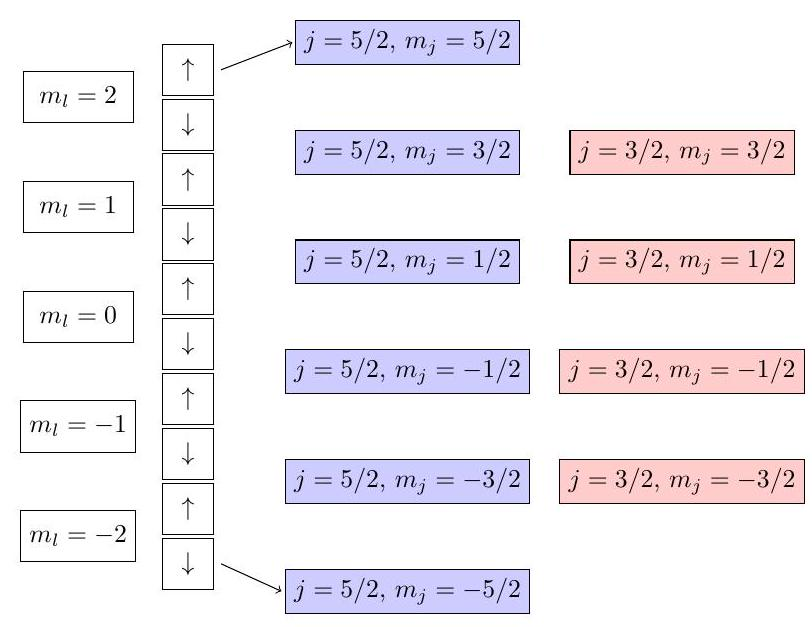
\includegraphics[max width=\textwidth]{2025_06_07_dbb046f06838039593f3g-09}
\end{center}

Figure 8.1: Kopplung von einem $l=2$ Bahndrehimpuls mit einen $S=1 / 2$ Spin. Es gibt jeweils 6 und 4 Zustände mit Gesamtdrehimpuls $5 / 2$ und $3 / 2$, also ingesamt $10=5 * 2$.\\
sind (wir vernachlässigen im folgdenden den Faktor $\hbar$ bei den Quantenzahlen der Drehimpulsoperatoren). Im Folenden betrachten wir ein festes $n$ und verwenden die DiracDarstellung,

$$
\psi_{ \pm}(\vec{x})=\left\langle\vec{x} \mid l, l_{3} ; S, S_{3}\right\rangle \quad\left(S=1 / 2, S_{3}= \pm 1 / 2\right)
$$

wobei $\left|l, l_{3} ; S, S_{3}\right\rangle$ der Basis-unabhängige Zustand zum Bahndrehimplus $l$ (z-Komponenten $l_{3}$ ) und dem Spin $S$ (z-Komponenten $S_{3}$ ) ist.

\subsubsection*{Gesamtdrehimpuls}
Der Gesamtdrehimpuls

$$
\overrightarrow{\mathbf{J}}=\overrightarrow{\mathbf{L}}+\overrightarrow{\mathbf{S}}, \quad \overrightarrow{\mathbf{J}}^{2}=\overrightarrow{\mathbf{L}}^{2}+\overrightarrow{\mathbf{S}}^{2}+2 \overrightarrow{\mathbf{L}} \cdot \overrightarrow{\mathbf{S}}
$$

ist eine gute Quantenzahl, $\left[\overrightarrow{\mathbf{J}}, \mathbf{H}_{0}+\mathbf{H}_{S B}\right]=0$, was man aus der Darstellung

$$
\mathbf{H}_{S B}=\frac{\lambda_{S B}}{2}\left(\overrightarrow{\mathbf{J}}^{2}-\overrightarrow{\mathbf{L}}^{2}-\overrightarrow{\mathbf{S}}^{2}\right)
$$

direkt ersieht, denn $\left[\overrightarrow{\mathbf{J}}, \overrightarrow{\mathbf{L}}^{2}\right]=0$ und $\left[\overrightarrow{\mathbf{J}}, \overrightarrow{\mathbf{S}}^{2}\right]=0$. Offentsichtlich genügt es nun, die möglichen Eigenwerte von $j(j+1)$ von $\overrightarrow{\mathbf{J}}^{2}$ zu kennen, um die Spin-Bahn-Kopplung diagonalisieren zu können.

\subsubsection*{Fragestellung}
Die Fragestellung lautet also: Gegeben seien zwei Drehimpulse $\mathbf{J}_{1}$ und $\mathbf{J}_{2}$, welche möglichen Werte hat der totale Drehimpuls $\mathbf{J}=\mathbf{J}_{1}+\mathbf{J}_{2}$ ? Allgemein wird dies Frage durch die Klebsch-Gordan Koeffizienten beantwortet ( $\rightarrow$ QM-2). Der hier relevante Fall, $\mathbf{J}_{1}=\mathbf{L}$ und $\mathbf{J}_{2}=\mathbf{S}$, läßt sich direkt behandeln. Das Ergebnis ist in Abbildung 4.1 dargestellt, wir werden es jetzt herleiten.\\
Eigenzustand von J mit $j=l+1 / 2$\\
Wir bezeichnen mit $\left|j, j_{3}\right\rangle$ die Eigenzustände von $\mathbf{J}$, mit $j_{3}=-j, \ldots, j$, Offensichtlich ist

$$
|l+1 / 2, l+1 / 2\rangle=|l, l ; S, 1 / 2\rangle
$$

ein Eigenzustand von $\mathbf{J}_{3}=\mathbf{L}_{3}+\mathbf{S}_{3}$ mit Eigenwerte $j_{3}=l+1 / 2$. Mit

$$
\mathbf{J}_{+}|l+1 / 2, l+1 / 2\rangle=0, \quad \mathbf{J}_{+}=\mathbf{L}_{+}+\mathbf{S}_{+}, \quad \mathbf{J}_{ \pm}=\mathbf{J}_{1} \pm i \mathbf{J}_{2}
$$

folgt, daß $j=l+1 / 2$ ist. Also haben wir schon mal einen möglichen Eigenwert von $\mathbf{J}^{2}$ gefunden. Gibt es noch weitere?

\subsubsection*{Absteige-Operation}
Mit Hilfe des Absteigeoperators

$$
\mathbf{J}_{-}\left|j, j_{3}\right\rangle=\sqrt{j(j+1)-j_{3}\left(j_{3}-1\right)}\left|j, j_{3}-1\right\rangle
$$

für den Gesamtdrehimpuls mit $j=l+1 / 2$ und $j_{3}=l+1 / 2$ finden wir zum Einen

$$
\begin{aligned}
\mathbf{J}_{-}\left|j, j_{3}\right\rangle & =\sqrt{(l+1 / 2)(l+3 / 2)-(l+1 / 2)(l-1 / 2)}\left|j, j_{3}-1\right\rangle \\
& =\sqrt{2 l+1}\left|j, j_{3}-1\right\rangle
\end{aligned}
$$

sowie

$$
\begin{aligned}
\mathbf{J}_{-}\left|j, j_{3}\right\rangle= & \left(\mathbf{L}_{-}+\mathbf{S}_{-}\right)|l, l ; S, 1 / 2\rangle \\
= & \sqrt{l(l+1)-l(l-1)}|l, l-1 ; S, 1 / 2\rangle \\
& \quad+\sqrt{1 / 2(1 / 2+1)-1 / 2(1 / 2-1)}|l, l ; S,-1 / 2\rangle \\
= & \sqrt{2 l}|l, l-1 ; S, 1 / 2\rangle+|l, l ; S,-1 / 2\rangle
\end{aligned}
$$

Zusammen ergibt sich die Darstellung

$$
|l+1 / 2, l-1 / 2\rangle=\frac{1}{\sqrt{2 l+1}}(\sqrt{2 l}|l, l-1 ; S, 1 / 2\rangle+|l, l ; S,-1 / 2\rangle)
$$

Eigenzustand von J mit $j=l-1 / 2$\\
Für $l>0$ existiert ein Zustand,

$$
|l-1 / 2, l-1 / 2\rangle=\frac{1}{\sqrt{2 l+1}}(|l, l-1 ; S, 1 / 2\rangle-\sqrt{2 l}|l, l ; S,-1 / 2\rangle,)
$$

der orthgonal zu $|l+1 / 2, l-1 / 2\rangle$ ist:

$$
\langle l+1 / 2, l-1 / 2 \mid l-1 / 2, l-1 / 2\rangle=\frac{2 l-2 l}{2 l+1}=0
$$

Für diesen Zustand gilt $j=l-1 / 2$, denn $\mathbf{J}_{+}|l-1 / 2, l-1 / 2\rangle=0$.\\
Es zeigt sich dass wir $j=l \pm 1 / 2$ nun schon alle möglichen Zustände für den Gesamtdrehimpuls konstruiert haben, wie in Abbildung 4.1 dargestell. Für den allgemeinen Klebsch-Gordan-Fall müsste man iterative weitere Zustände berechnen.

\subsubsection*{Anzahl der Zustände}
Um die zu zeigen, dass $j=l \pm 1 / 2$ die beiden einzig möglichen Werte für den Gesamtdrehimpuls sind, berechnen wir die Gesamtzahl der gefundenen Zustände,

$$
\sum_{j}(2 j+1)=2\left(l+\frac{1}{2}\right)+1+2\left(l-\frac{1}{2}\right)+1=4 l+2=(2 l+1) 2
$$

Dies ist also identisch mit der Gesamtanzahl der Zustände $(2 l+1) 2$ des Produkt-HilbertRaumes (vom Banhdrehimpuls $\mathbf{L}$ mit Entartung $2 l+1$ und vom Spin mit Entartung $2 S+1=2$ ). Wir haben also alle möglichen Eigenwerte von $\mathbf{J}=\mathbf{L}+\mathbf{S}$ gefunden.

\subsubsection*{Gestörte Energien}
Für die Spin-Bahn-Kopplung erhalten wir (jetzt wieder mit dem Faktor $\hbar^{2}$ )

$$
\begin{aligned}
\overrightarrow{\mathbf{L}} \cdot \overrightarrow{\mathbf{S}}\left|n ; j, j_{3}\right\rangle & =\frac{\hbar^{2}}{2}[j(j+1)-l(l+1)-s(s+1)]\left|n ; j, j_{3}\right\rangle \\
& =\left\{\begin{array}{rr}
\frac{\hbar^{2}}{2} l\left|n ; j, j_{3}\right\rangle & \text { für } \quad j=l+\frac{1}{2} \\
\frac{\hbar^{2}}{2}(-l-1)\left|n ; j, j_{3}\right\rangle & \text { für } \quad j=l-\frac{1}{2}
\end{array}\right.
\end{aligned}
$$

wobei wir $(\overrightarrow{\mathbf{L}}+\overrightarrow{\mathbf{S}})^{2}=\overrightarrow{\mathbf{L}}^{2}+2 \overrightarrow{\mathbf{L}} \cdot \overrightarrow{\mathbf{S}}+\overrightarrow{\mathbf{S}}^{2}$ verwendet haben. Für die Enerige $\lambda E_{n l j}^{(1)}$ folgt daraus in 1. Näherung:

$$
\lambda E_{n l j}^{(1)}=-\frac{e}{2 m_{e}^{2} c^{2}} \frac{\hbar^{2}}{2}\left\langle n ; j, j_{3}\right| \frac{1}{r} \frac{d \varphi}{d r}\left|n ; j, j_{3}\right\rangle \cdot\left\{\begin{array}{c}
l \\
-l-1
\end{array}\right.
$$

Für $l \neq 0$ erhält man also eine Aufspaltung der Energie-Niveaus, welche zu $j=l+\frac{1}{2}$ und $j=l-\frac{1}{2}$ gehören.

\subsubsection*{Relative Stärke der Spin-Bahnkopplung}
Um die Grössenordnung abzuschätzen benutzen wir

$$
\varphi(r)=\frac{e Z}{4 \pi \varepsilon_{0} r}, \quad \frac{1}{r} \frac{d \varphi}{d r}=-\frac{e Z}{4 \pi \varepsilon_{0} r^{3}} \approx-\frac{e Z}{4 \pi \varepsilon_{0} a_{0}^{3}}, \quad \quad E_{0} \approx-\frac{1}{2} \frac{e^{2} Z}{4 \pi \varepsilon_{0} a_{0}}
$$

mit dem Bohrschen Radius $a_{0}=4 \pi \epsilon_{0} \hbar^{2} /\left(m_{e} e^{2}\right)$. Damit erhalten wir

$$
\frac{W_{S B}}{E_{0}} \approx \frac{e}{2 m_{e}^{2} c^{2}} \frac{\hbar^{2}}{2} \frac{2}{e a_{0}^{2}}=\frac{\hbar^{2}}{2 c^{2}}\left(\frac{e^{2}}{4 \pi \epsilon_{0} \hbar^{2}}\right)^{2}=\frac{1}{2}\left(\frac{e^{2}}{4 \pi \epsilon_{0} \hbar c}\right)^{2}=\frac{1}{2} \alpha^{2} \approx \frac{1}{2} \frac{1}{137^{2}}
$$

für den Quotienten zwischen der Spin-Bahn Korrektur $W_{S B}$ und der Grundzustandsenergie $E_{0}$, mit der Feinstrukuturkonstanten $\alpha=e^{2} /\left(e \pi \epsilon_{0} \hbar c\right) \approx 1 / 137$.

\subsubsection*{D-Linie}
Ein bekanntes Beispiel bildet die Aufspaltung der gelben "D-Linie" des Natriums. Sie entspricht den Übergängen $(l=1) \rightarrow(l=0)$. Das obere Niveau ist entsprechend $j=\frac{1}{2}$\\
und $j=\frac{3}{2}$ aufgespalten. Die Linien gehören zu $n=3$. Man beachte, dass bei den AlkaliSpektren schon die ungestörten Niveaus von $l$ abhängig sind, da das Coulomb-Potential wegen der Abschirmung durch die inneren Elektronen modifiziert ist.

\subsubsection*{Weitere Korrekturen}
Die Energie-Niveaus im Wasserstoffatom werden durch weitere Effekte beinflusst.

\begin{itemize}
  \item Relativistische Korrekturen
\end{itemize}

$$
\begin{aligned}
E_{k i n} & \left.=m c^{2} \sqrt{1+\frac{\vec{p}^{2}}{m^{2} c^{2}}}\right)-m c^{2} \\
& =\frac{\vec{p}^{2}}{2 m}-\frac{1}{8 m^{3} c^{2}}\left(\vec{p}^{2}\right)^{2}+\cdots
\end{aligned}
$$

Spin-Bahn-Kopplung und relativistische Korrekturen werden automatisch in der Dirac-Gleichung berücksichtigt.

\begin{itemize}
  \item Hyperfeinstruktur
\end{itemize}

Wechselwirkung des magnetischen Momentes vom Proton mit dem vom Elektron.

\begin{itemize}
  \item Ausdehnung des Protons
\end{itemize}

Die kleine aber endliche Ausdehnung des Kerns führ zu Modifikationen der Wellenfunktion für $r \rightarrow 0$.

\begin{itemize}
  \item Elektromagnetische Nullpunktsschwingungen
\end{itemize}

Wechselwirkung des Elektrons mit dem "Strahlungsfeld", d.h. dem elektromagnetischen Fluktuationen des Vakuums.\\
Diese führt zum Lamb-shift (Aufspaltung von auch bei der Dirac-Gleichung noch entarteten Energie-Niveaus) und Korrekturen zu $g=2$. (Quantenelektrodynamik)

\pagebreak


\section{Zeitentwicklung und Symmetrien}



\subsection*{Zeitliche Entwicklung von Zuständen und Operatoren}
Ohne zeitliche Entwicklung gibt es keine Prozesse in dieser Welt. In der Quantenmechanik kann man die Zeitentwicklung entweder in die Wellenfunktionen oder in die Operatoren stecken, oder in beide.

\subsubsection*{Zeitunabhängige Operatoren}
Wir betrachten zunächst einzelne Teilchen in einem Potential $V(\vec{x})$, das selber nicht explizit von der Zeit abhängen soll. Die Schrödinger'sche Wellenfunktion $\psi(\vec{x}, t)$ genügt der Gleichung

$$
i \hbar \frac{d}{d t} \psi(\vec{x}, t)=\mathbf{H} \psi(\vec{x}, t) \quad \mathbf{H}=-\frac{\hbar^{2}}{2 m_{e}} \Delta+V(\vec{x})
$$

Die Operatoren $\mathbf{Q}_{j}=$ Multiplikation mit $x_{j}$ sowie $\mathbf{P}_{j}=\frac{\hbar}{i} \frac{\partial}{\partial x_{j}}$ sind zeitunabhängig, die Zeitabhängigkeit steht in $\psi(\vec{x}, t)$.

\subsubsection*{Zeitabhängige Operatoren}
Es gibt Operatoren welche explizit von der Zeit abhängen. Sei z.B. $\mathbf{A}=\mathbf{A}(\overrightarrow{\mathbf{P}}, \overrightarrow{\mathbf{Q}}, t)$ ein Operator, der von $\overrightarrow{\mathbf{P}}, \overrightarrow{\mathbf{Q}}$ und explizit von der Zeit $t$ abhängen kann, z.B. wie

$$
\mathbf{A}=\overrightarrow{\mathbf{Q}}-\frac{1}{m} \overrightarrow{\mathbf{P}} \cdot t
$$

Klassisch entspricht $p / m=v$ der Geschwindigkeit, der Operator A entspricht also in diesem Beispiel dem relativen Aufenhaltsort eines sich frei bewegenden Teilchens.

\subsubsection*{Erwartungswerte}
Für den zeitabhängigen Erwartungswert $\langle\mathbf{A}\rangle_{\psi}(t) \equiv\langle\psi(t)| \mathbf{A}|\psi(t)\rangle$ führt die Schrödingergleichung zu

$$
\begin{aligned}
\frac{d}{d t}\langle\mathbf{A}\rangle_{\psi}(t) & =\langle\dot{\psi}| \mathbf{A}|\psi\rangle+\langle\psi| \dot{\mathbf{A}}|\psi\rangle+\langle\psi| \mathbf{A}|\dot{\psi}\rangle \\
& =-\frac{1}{i \hbar}\langle\psi| \mathbf{H A}|\psi\rangle+\frac{1}{i \hbar}\langle\psi| \mathbf{A H}|\psi\rangle+\left\langle\partial_{t} \mathbf{A}\right\rangle_{\psi}
\end{aligned}
$$

da $\mathbf{H}$ selbstadjungiert ist. Es gilt somit

$$
\frac{d}{d t}\langle\mathbf{A}\rangle_{\psi}(t)=\frac{i}{\hbar}\langle\psi|[\mathbf{H}, \mathbf{A}]|\psi\rangle+\left\langle\partial_{t} \mathbf{A}\right\rangle_{\psi}
$$

hier mit der Abkürzung $\partial_{t}=\partial / \partial t$. Dieses ist die grundlegende Bewegungsgleichung für Operatoren.

\subsubsection*{Beispiel}
Sei $\mathbf{A}=\overrightarrow{\mathbf{P}}=\frac{\hbar}{i}$ grad, dann gilt $\partial_{t} \overrightarrow{\mathbf{P}}=0$ und

$$
\begin{aligned}
{[\mathbf{H}, \overrightarrow{\mathbf{P}}] } & =[V(\vec{x}), \overrightarrow{\mathbf{P}}]=V(\vec{x}) \overrightarrow{\mathbf{P}}-\overrightarrow{\mathbf{P}}(V(\vec{x})) \\
& =-\frac{\hbar}{i}(\operatorname{grad} V(\vec{x}))
\end{aligned}
$$

Hieraus folgt mit

$$
\frac{d}{d t}\langle\overrightarrow{\mathbf{P}}\rangle_{\psi}=-\langle\operatorname{grad} V\rangle_{\psi}
$$

das Analogon zur Newton'schen Bewegungsgleichung $\frac{d}{d t} \vec{p}=-\operatorname{grad} V$.\\
Erwartungswerte erfüllen das Korrespondenzprinzip.

\subsubsection*{Zeitentwicklungsoperator}
Sei $u_{0}(\vec{x})$ der Zustand des Teilchens zur Zeit $t=0$ (Anfangswertproblem). Dabei muß $u_{0}(\vec{x})$ nicht notwendigerweise ein Eigenzustand von $\mathbf{H}$ sein, welcher zeitunabhängig sein soll: $\partial_{t} \mathbf{H}=0$.\\
Das Anfangswertproblem

$$
i \hbar \frac{\partial}{\partial t} \psi(\vec{x}, t)=\mathbf{H} \psi(\vec{x}, t), \quad \psi(\vec{x}, t=0) \equiv \psi_{0}(\vec{x})=u_{0}(\vec{x})
$$

hat die (formale) Lösung

$$
\psi(\vec{x}, t)=e^{-i \mathbf{H} t / \hbar} u_{0}(\vec{x}) \equiv \sum_{n=0}^{\infty}\left(\frac{-i t}{\hbar}\right)^{n} \frac{\mathbf{H}^{n}}{n!} u_{0}(\vec{x})
$$

Beweis :

$$
\begin{aligned}
i \hbar \frac{d}{d t} \psi(\vec{x}, t) & =\sum_{n=0}^{\infty} n\left(\frac{-i t}{\hbar}\right)^{n-1} \frac{\mathbf{H}^{n}}{n!} u_{0}(\vec{x}) \\
& =\sum_{m=0}^{\infty}\left(\frac{-i t}{\hbar}\right)^{m} \frac{\mathbf{H}^{m+1}}{m!} u_{0}(\vec{x})=\mathbf{H} \psi(\vec{x}, t)
\end{aligned}
$$

wobei wir die Substitution $m+1=n$ vorgenommen haben. Die Transformation

$$
\psi(\vec{x}, 0)=u_{0}(\vec{x}) \quad \rightarrow \quad \psi(\vec{x}, t)=U(-t) u_{0}(\vec{x})
$$

definiert mit

$$
U(t)=e^{i \mathbf{H} t / \hbar}
$$

den Zeitentwicklungsoperator $U(t)$.

\subsubsection*{Unitarität}
Das Skalarprodukt

$$
\begin{aligned}
\langle\psi(t) \mid \phi(t)\rangle & =\langle\psi(0)| U^{+}(-t) U(-t)|\phi(0)\rangle=\langle\psi(0)| e^{i \mathbf{H} t / \hbar} e^{-i \mathbf{H} t / \hbar}|\phi(0)\rangle \\
& =\langle\psi(0) \mid \phi(0)\rangle
\end{aligned}
$$

bleibt unter der Zeitentwicklung erhalten und somit auch die Norm. $U(t)$ ist somit unitär:

$$
U^{+}(t) U(t)=U(t) U^{+}(t)=1
$$

\subsubsection*{Zeitentwicklung von Operatoren}
Setzt man $\psi(\vec{x}, t)=U(-t) \psi_{0}(\vec{x})$ in den Erwartungswert $\langle\mathbf{A}\rangle_{\psi}$ ein, so erhält man

$$
\langle\mathbf{A}\rangle_{\psi}(t)=\langle\psi(t)| \mathbf{A}|\psi(t)\rangle=\langle\psi(0)| e^{+i t \mathbf{H} / \hbar} \mathbf{A} e^{-i t \mathbf{H} / \hbar}|\psi(0)\rangle .
$$

Dieser Ausdruck legt es nahe, zeitabhängige Operatoren

$$
\tilde{\mathbf{A}}(t)=U(t) \mathbf{A} U^{+}(t) \quad U(t)=e^{i t \mathbf{H} / \hbar}
$$

zu definieren.

\subsubsection*{Bewegungsgleichung von Operatoren}
Aus $i \hbar \frac{d}{d t} U(t)=-\mathbf{H} U(t)$ folgt mit

$$
i \hbar \frac{d}{d t} \tilde{\mathbf{A}}(t)=\underbrace{-\mathbf{H} \tilde{\mathbf{A}}(t)+\tilde{\mathbf{A}}(t) \mathbf{H}}_{[\tilde{\mathbf{A}}, \mathbf{H}]}+i \hbar \underbrace{U(t) \partial_{t} \mathbf{A} U^{+}(t)}_{\equiv \partial_{t} \tilde{\mathbf{A}}}
$$

die Bewegungsgleichung für den Operator $\mathbf{A}$, wobei wir mit $\partial_{t} \tilde{\mathbf{A}}$ im folgenden die Ableitung nach der expliziten Zeitabhängigkeit des Operators $\mathbf{A}$ bezeichnen. Diese Bewegungsgleichung, $i \hbar d t \tilde{\mathbf{A}} / d t=[\tilde{\mathbf{A}}, \mathbf{H}]+i \hbar \partial_{t} \tilde{\mathbf{A}}$, ist analog zu jener für die Erwartungswerte von Operatoren.

\subsubsection*{Schrödinger $\leftrightarrow$ Heisenberg Bild}
Wir haben zwei Möglichkeiten der Beschreibung zeitabhängiger Erwartungswerte, hier für den Fall $\partial_{t} \mathbf{A}=0$ :

\subsubsection*{Schrödinger-Bild}
Die Operatoren sind zeitunabhängig und die Zeitabhängigkeit steckt in den Zuständen $\psi(\vec{x}, t)$, deren zeitliche Entwicklung durch $i \hbar \partial_{t} \psi=\mathbf{H} \psi$ gegeben ist.

\subsubsection*{Heisenberg-Bild}
Die Zustände $\psi_{0}(\vec{x})$ sind zeitunabhängig, dafür hängen Operatoren $\tilde{\mathbf{A}}(t)$ von der Zeit ab. Die Bewegungsgleichung für Operatoren ist

$$
i \hbar \frac{d}{d t} \tilde{\mathbf{A}}(t)=[\tilde{\mathbf{A}}(t), \mathbf{H}] .
$$

\subsubsection*{Invarianz der Observablen}
Beide "Bilder" führen zu den selben Messgrößen, denn die Erwartungswerte

$$
\langle\psi(t)| \mathbf{A}|\psi(t)\rangle=\langle\psi(0)| \tilde{\mathbf{A}}(t)|\psi(0)\rangle
$$

bleiben bei einem Wechsel von der Schrödinger- zur Heisenberg-Darstellung nach Konstruktion invariant. Zur Zeit $t=0$ stimmen Zustände und Operatoren im Heisenberg- und Schrödinger-Bild überein. Da der Hamilton-Operator $\mathbf{H}$ mit $U(t)=e^{i t \mathbf{H} / \hbar}$ vertauscht, gilt allgemein $\tilde{\mathbf{H}}=\mathbf{H}$.

\subsubsection*{Harmonischer Oszillator}
Als Beispiel betrachten wir den harmonischen Oszillator

$$
\mathbf{H}=\hbar \omega\left(\mathbf{a}^{+} \mathbf{a}+\frac{1}{2}\right) \quad\left[\mathbf{a}, \mathbf{a}^{+}\right]=1,
$$

mit den Auf- und Absteigeoperatoren $\mathbf{a}^{+}$und $a$. Es gilt

$$
\left[\mathbf{a}^{+}, \mathbf{H}\right]=\hbar \omega\left(\mathbf{a}^{+} \mathbf{a}^{+} \mathbf{a}-\mathbf{a}^{+} \mathbf{a a}^{+}\right)=\hbar \omega \mathbf{a}^{+}\left[\mathbf{a}^{+}, \mathbf{a}\right]=-\hbar \omega \mathbf{a}^{+} .
$$

Wir multiplizieren von links mit $U(t)$ und von rechts mit $U(-t)=U^{+}(t)$. Wegen

$$
U(t) U(-t)=1, \quad \tilde{\mathbf{a}}^{+}=U(t) \mathbf{a}^{+} U(-t), \quad \tilde{\mathbf{H}}=\mathbf{H},
$$

ergibt sich

$$
\left[U(t) \mathbf{a}^{+} U(-t), U(t) \mathbf{H} U(-t)\right]=\left[\tilde{\mathbf{a}}^{+}(t), \mathbf{H}\right]=-\hbar \omega \tilde{\mathbf{a}}^{+} .
$$

Also

$$
i \hbar \frac{d \tilde{\mathbf{a}}^{+}(t)}{d t}=\left[\tilde{\mathbf{a}}^{+}(t), \mathbf{H}\right]=-\hbar \omega \tilde{\mathbf{a}}^{+}(t)
$$

Da die Bewegungsgleichungen für $\tilde{\mathbf{a}}(t)$ und $\tilde{\mathbf{a}}^{+}(t)$ zueinander konjungiert-komplex sind, erhalten wir somit

$$
\frac{d \tilde{\mathbf{a}}^{+}(t)}{d t}=i \omega \tilde{\mathbf{a}}^{+}(t) \quad \frac{d \tilde{\mathbf{a}}(t)}{d t}=-i \omega \tilde{\mathbf{a}}(t)
$$

Diese Operator-Differentialgleichungen haben die Lösungen:

$$
\begin{aligned}
\tilde{\mathbf{a}}^{+}(t) & =e^{i \omega t} \tilde{\mathbf{a}}^{+}(0) & \tilde{\mathbf{a}}^{+}(0) & =\mathbf{a}^{+} \\
\tilde{\mathbf{a}}(t) & =e^{-i \omega t} \tilde{\mathbf{a}}(0) & \tilde{\mathbf{a}}(0) & =\mathbf{a}
\end{aligned}
$$

\subsubsection*{Observable}
Für den Ort- und Impuls-Operator,

$$
\tilde{\mathbf{Q}}(t)=\frac{1}{\sqrt{2} \beta}\left(\tilde{\mathbf{a}}(t)+\tilde{\mathbf{a}}^{+}(t)\right), \quad \tilde{\mathbf{P}}(t)=\frac{\hbar}{i} \frac{\beta}{\sqrt{2}}\left(\tilde{\mathbf{a}}(t)-\tilde{\mathbf{a}}^{+}(t)\right), \quad \beta^{2}=\frac{m \omega}{\hbar},
$$

ergibt sich

$$
\begin{aligned}
\tilde{\mathbf{Q}}(t) & =\frac{1}{\sqrt{2} \beta}\left(e^{i \omega t} \tilde{\mathbf{a}}^{+}(0)+e^{-i \omega t} \tilde{\mathbf{a}}(0)\right) \\
& =\frac{\cos \omega t}{\sqrt{2} \beta}\left(\tilde{\mathbf{a}}^{+}(0)+\tilde{\mathbf{a}}(0)\right)+\frac{i \sin \omega t}{\sqrt{2} \beta}\left(\tilde{\mathbf{a}}^{+}(0)-\tilde{\mathbf{a}}(0)\right)
\end{aligned}
$$

Wir erhalten also mit

$$
\begin{aligned}
\tilde{\mathbf{Q}}(t) & =\mathbf{Q}(0) \cos \omega t+\frac{1}{m \omega} \mathbf{P}(0) \sin \omega t \\
\tilde{\mathbf{P}}(t) & =\mathbf{P}(0) \cos \omega t-m \omega \mathbf{Q}(0) \sin \omega t
\end{aligned}
$$

die klassische Lösung des harmonischen Oszillators (eine Ellipse im Zustandsraum). Eine alternative Herleitung benutzt kohärente Zustände, welche im Abschnitt ?? diskutiert wurden.

\subsubsection*{Konstanten der Bewegung}
Aus der klassichen Mechanik wissen wir, dass jede (zeitunabhängige) Funktion auf dem Phasenraum $F(P, Q)$ genau dann eine Konstante der Bewegung ist, also eine Erhaltungsgrösse, wenn die Poisson-Klammer von $F$ und der Hamilton-Funktion verschwindet.

Quantenmechanisch gilt:

$$
\frac{d}{d t} \tilde{\mathbf{A}}(t)=0, \quad \text { falls } \quad[\mathbf{H}, \tilde{\mathbf{A}}(t)]=0 \quad \text { und } \quad \partial_{t} \mathbf{A}=0
$$

Jeder Operator $\tilde{\mathbf{A}}(t)$, (bzw. A), der mit $\mathbf{H}$ vertauscht, ist eine Konstante der Bewegung, liefert also einen Erhaltungssatz.

Somit geht im Rahmen des Korrespondenzprinzips die Poisson-Klammer der klassischen Mechanik in den Kommutator der Quantenmechanik über. Dies wurde schon im Abschnitt ?? erwähnt.

\subsubsection*{Kanonische Gleichungen}
Im Heisenberg-Bild genügen die Operatoren $\tilde{\mathbf{Q}}_{j}(t)$ und $\tilde{\mathbf{P}}_{j}(t)$ den "kanonischen" OperatorGleichungen

$$
\frac{d}{d t} \tilde{\mathbf{Q}}_{j}(t)=\frac{\partial \mathbf{H}}{\partial \tilde{\mathbf{P}}_{j}(t)} \quad \frac{d}{d t} \tilde{\mathbf{P}}_{j}(t)=-\frac{\partial \mathbf{H}}{\partial \tilde{\mathbf{Q}}_{j}(t)}
$$

Diese Gleichungen folgen direkt aus dem Korrespondenzprinzip, man kann sie natürlich auch mit Hilfe der Bewegungsgleichung und der Vertauschungsrelationen

$$
i \hbar \frac{d}{d t} \tilde{\mathbf{A}}(t)=[\tilde{\mathbf{A}}(t), \mathbf{H}] \quad \text { und } \quad\left[\tilde{\mathbf{P}}_{j}(t), \tilde{\mathbf{Q}}_{k}(t)\right]=\frac{\hbar}{i} \delta_{j k}
$$

herleiten.

\subsubsection*{Wechselwirkungsbild}
Es sei $\mathbf{H}=\mathbf{H}_{0}+\mathbf{W}$, wobei $\mathbf{H}_{0}$ das System ohne Wechselwirkung (Störung) $\mathbf{W}$ beschreibt. Um das volle System approximativ zu lösen, möchte man nun ausnutzten, dass die Eigenzustände von $\mathbf{H}_{0}$ bekannt sind.

\begin{itemize}
  \item Schrödinger Bild
\end{itemize}

Die Wellenfunktion ist eine Funktion der Zeit, Operatoren nicht (falls ein Operator nicht explizit von der Zeit abhängt).

\begin{itemize}
  \item Heisenberg Bild
\end{itemize}

Die Wellenfunktion ist nicht Zeit-abhängig, nur Operatoren.

\begin{itemize}
  \item Wechselwirkungs-Bild
\end{itemize}

Die Zeit-Abhängigkeit der Wellenfunktion wird durch die Wechselwirkung W bestimmt, die der Operatoren von $\mathbf{H}_{0}$ (modulo explizite Zeitabhängigkeiten).

Im Schrödinger-Bild werden Zustände durch

$$
\psi(\vec{x}, t)=U(-t) \psi_{0}(\vec{x})
$$

beschrieben. Man kann nun die zeitliche Entwicklung von $\psi(\vec{x}, t)$ relativ zu $\mathbf{H}_{0}$ rückwärts verfolgen und

$$
\widehat{\psi}(\vec{x}, t)=e^{i t \mathbf{H}_{0} / \hbar} \psi(\vec{x}, t)=e^{i t \mathbf{H}_{0} / \hbar} U(-t) \psi_{0}(\vec{x})
$$

definieren. Man nennt $\widehat{\psi}(\vec{x}, t)$ die Wellenfunktion im Wechselwirkungsbild. Die Operatoren $\widehat{\mathbf{A}}(t)$ im Wechselwirkungsbild definieren wir entsprechend via

$$
\widehat{\mathbf{A}}(t)=e^{i \mathbf{H}_{0} t / \hbar} \mathbf{A} e^{-i \mathbf{H}_{0} t / \hbar}
$$

Erwartungswerte bleiben nach Konstruktion invariant,

$$
\langle\widehat{\psi}(t)| \widehat{\mathbf{A}}(t)|\widehat{\psi}(t)\rangle=\langle\psi(t)| \mathbf{A}|\psi(t)\rangle=\left\langle\psi_{0}\right| \tilde{\mathbf{A}}(t)\left|\psi_{0}\right\rangle
$$

Die Bewegungsgleichungen (für $\partial_{t} \mathbf{A}=0$ ) sind jetzt:

$$
\begin{aligned}
i \hbar \frac{d}{d t} \widehat{\mathbf{A}} & =\left[\widehat{\mathbf{A}}(t), \mathbf{H}_{0}\right] \\
i \hbar \partial_{t} \widehat{\psi}(\vec{x}, t) & =\widehat{\mathbf{W}}(t) \widehat{\psi}(\vec{x}, t)
\end{aligned}
$$

Das Wechselwirkungsbild spielt eine wichtige Rolle in der zeitabhängigen Störungstheorie. In dieser ist $\mathbf{H}_{0}$ bekannt und die Störung typischerweise ein Messvorgang. Da die Zeitentwicklung, welche aus der Störung resultiert, im Wechelwirkungsbild separat auftritt, kann man im Wechelwirkungsbild direckt nach Potenzen in $\widehat{\mathbf{W}}$ entwicklen.

\subsection*{Translationen, Drehungen und Galilei-Invarianz}
Die zeitliche Entwicklung einer Wellenfunktion von $t$ zu $t+\tau$,

$$
\psi \quad \rightarrow \quad \psi(\vec{x}, t+\tau)=e^{-i \tau \mathbf{H} / \hbar} \psi(\vec{x}, t),
$$

hier im Schrödinger Bild, kann man auch als eine Translatione in der Zeit auffassen. Analog betrachten wir nun räumlichen Translationen $\vec{x} \rightarrow \vec{x}+\vec{a}$.

\subsubsection*{Räumliche Translationen}
\subsubsection*{Erzeugende von Transformationen}
Bei räumlichen Translationen wird die Verschiebung des Koordinantenurspungs um einen konstanten Vekotr $\vec{a}$ durch den Operator $U(\vec{a})$ bewirkt, mit

$$
U(\vec{a}) u(\vec{x})=u(\vec{x}+\vec{a}) \quad U(\vec{a})=e^{i \vec{a} \cdot \overrightarrow{\mathbf{P}} / \hbar}
$$

wobei $u(\vec{x})$ die Wellenfunktion ist (beliebig oft differenzierbar), und $\overrightarrow{\mathbf{P}}=\hbar \vec{\nabla} / i$ der Impulsoperator. Wegen dieser Exponentialdarstellung nennt man $\overrightarrow{\mathbf{P}}$ die Erzeugende des Translationsoperators.

\subsubsection*{Fall einer Dimension}
Für den Beweis betrachten wir den Fall einer räumlichen Dimension,

$$
U(a) u(x)=e^{i a \mathbf{P} / \hbar} u(x)=\sum_{n} \frac{a^{n}}{n!} \frac{\partial^{n}}{\partial^{n} x} u(x)=u(x+a)
$$

wobei wir im letzten Schritt die Definition der Taylor-Entwicklung benutzt haben.

\subsubsection*{Unitarität}
Mit

$$
(U(\vec{a}) u(\vec{x}), U(\vec{a}) u(\vec{x}))=\int d^{3} \vec{x} u^{*}(\vec{x}+\vec{a}) u(\vec{x}+\vec{a})=\int d^{3} \vec{x} u^{*}(\vec{x}) u(\vec{x})=(u(\vec{x}), u(\vec{x}))
$$

ist das Sklarprodukt erhalten. Räumliche Translationen,

$$
u(\vec{x}) \quad \rightarrow \quad U(\vec{a}) u(\vec{x})=e^{i \vec{a} \cdot \overrightarrow{\mathbf{P}} / \hbar} u(\vec{x})
$$

entsprechen daher unitären Transformationen.

\subsubsection*{N-Teilchen Wellenfunktion}
Bei $N$ Teilchen hat der Gesamtimpuls-Operator die Form

$$
\overrightarrow{\mathbf{P}}=\frac{\hbar}{i} \sum_{n=1}^{N} \vec{\nabla}_{n} \quad \text { mit } \quad u=u\left(\vec{x}_{1}, \ldots, \vec{x}_{N}\right)
$$

Alle $N$ Koordinaten $\vec{x}_{n}$ müssen gleichzeitig transformiert werden:

$$
U(\vec{a}) u\left(\vec{x}_{1}, \ldots, \vec{x}_{N}\right)=e^{i \vec{a} \cdot \overrightarrow{\mathbf{P}} / \hbar} u\left(\vec{x}_{1}, \ldots, \vec{x}_{N}\right)=u\left(\vec{x}_{1}+\vec{a}, \ldots, \vec{x}_{N}+\vec{a}\right)
$$

\subsubsection*{Gesamtimpuls-Erhaltung}
Es sei nun

$$
\mathbf{H}=\sum_{n=1}^{N} \frac{-\hbar^{2}}{2 m_{n}} \Delta_{n}+\frac{1}{2} \sum_{j \neq k} V_{j k}\left(\vec{x}_{j}-\vec{x}_{k}\right),
$$

dann folgt wegen der Translations-Invarianz von $\mathbf{H}$ aus

$$
\begin{aligned}
\mathbf{H} u\left(\vec{x}_{1}, \ldots, \vec{x}_{N}\right) & =E u\left(\vec{x}_{1}, \ldots, \vec{x}_{N}\right) \\
\mathbf{H} u\left(\vec{x}_{1}-\vec{a}, \ldots, \vec{x}_{N}-\vec{a}\right) & =E u\left(\vec{x}_{1}-\vec{a}, \ldots, \vec{x}_{N}-\vec{a}\right)
\end{aligned}
$$

daß

$$
\mathbf{H} U(-\vec{a}) u\left(\vec{x}_{1}, \ldots, \vec{x}_{N}\right)=E U(-\vec{a}) u\left(\vec{x}_{1}, \ldots, \vec{x}_{N}\right) .
$$

Multiplikation von links mit $U(\vec{a})$ ergibt

$$
\begin{aligned}
U(\vec{a}) \mathbf{H} U(-\vec{a}) u\left(\vec{x}_{1}, \ldots, \vec{x}_{N}\right) & =U(\vec{a}) E U(-\vec{a}) u\left(\vec{x}_{1}, \ldots, \vec{x}_{N}\right)=E u\left(\vec{x}_{1}, \ldots, \vec{x}_{N}\right) \\
& =\mathbf{H} u\left(\vec{x}_{1}, \ldots, \vec{x}_{N}\right)
\end{aligned}
$$

Da diese Beziehung für alle Eigenfunktionen des selbstadjungierten Operators $\mathbf{H}$ gelten soll, hat man

$$
U(\vec{a}) \mathbf{H} U(-\vec{a})=\mathbf{H}, \quad U(\vec{a}) \mathbf{H}-\mathbf{H} U(\vec{a})=0
$$

Der Hamilton-Operator vertauscht also mit allen Translationen. Dieser Zusammenhang gilt für alle Symmetrien.

\subsubsection*{Infinitesimale Translationen}
Entwickelt man $U(\vec{a})=\exp (i \vec{a} \cdot \overrightarrow{\mathbf{P}} / \hbar)$ nach Potenzen von $\vec{a}$ bis zur Ordnung $\vec{a}$, so erhält man

$$
(1+i \vec{a} \cdot \overrightarrow{\mathbf{P}} / \hbar) \mathbf{H}-\mathbf{H}(1+i \vec{a} \cdot \overrightarrow{\mathbf{P}} / \hbar)=0
$$

für kleinen $\vec{a}$, und damit

$$
\mathbf{H} \mathbf{P}_{j}-\mathbf{P}_{j} \mathbf{H}=\left[\mathbf{H}, \mathbf{P}_{j}\right]=0 \quad j=1,2,3
$$

Der Gesamtimpuls $\overrightarrow{\mathbf{P}}$ vertauscht also mit $\mathbf{H}$, und ist demnach eine Konstante der Bewegung (Erhaltungssatz). Dieser Zusammenhang gilt allgemein:

Invarianz unter Symmetrien\\
Ein Operator A ist invariant unter einer Symmetrie dann und nur dann wenn er mit der Erzeugenden E der Symmetrie vertauscht, also wenn $[\mathbf{A}, \mathbf{E}]=0$.

In unserem obrigen Beispiel war $\mathbf{A}=\mathbf{H}$ und $\mathbf{E}=\overrightarrow{\mathbf{P}}$.

\subsubsection*{Drehungen}
Wir errinnern an die Definition der Drehimpuls Operatoren,

$$
\overrightarrow{\mathbf{L}}=\overrightarrow{\mathbf{x}} \times \overrightarrow{\mathbf{P}}, \quad \mathbf{L}_{j}=\frac{\hbar}{i} \epsilon_{j k l} \mathbf{x}_{k} \partial_{l}
$$

Drehungen $\vec{x} \rightarrow R_{\vec{n}}(\varphi) \vec{x}$ sind durch zwei Grössen definiert:

\begin{itemize}
  \item $\varphi$, der Drehwinkel einer Drehung, und
  \item $\vec{n}$, die Drehachse, mit $\vec{n}^{2}=1$.
\end{itemize}

Man kann auch beides zu $\vec{\varphi}=\varphi \vec{n}$ zusammenfassen. Analog schreibt man $R_{\vec{\varphi}}=R_{\vec{n}}(\varphi)$ für die $3 \times 3$ Dreh-Matrizen.

\subsubsection*{Erzeugende für Drehungen}
War der Impuls die Erzeugenden für Tranlationen, sind die Drehimpuls-Operatoren analog die Erzeugende für endliche Drehungen.

Ist $\psi(\vec{x}, t)$ die Wellenfunktion eines spinlosen Teilchen, so gilt

$$
\begin{aligned}
U(\vec{\varphi}) \psi(\vec{x}, t) & \equiv e^{i \overrightarrow{\mathbf{L}} \cdot \vec{\varphi} / \hbar} \psi(\vec{x}, t) \\
& =\psi\left(R_{\vec{\varphi}} \vec{x}, t\right)
\end{aligned}
$$

Der Beweis lässt sich analog zu Translationen führen (Taylor-Reihe), ist rechentechnisch aber etwas aufwendiger.

\subsubsection*{Norm}
Die $3 \times 3$ Drehmatrix $R_{\vec{\varphi}}$ erhält die Norm,

$$
\begin{aligned}
\int d^{3} \vec{x} \psi^{*}\left(R_{\vec{\varphi}} \vec{x}, t\right) \psi\left(R_{\vec{\varphi}} \vec{x}, t\right) & =\int d^{3}\left(R_{n}^{-1}(\varphi) \vec{x}\right) \psi^{*}(\vec{x}, t) \psi(\vec{x}, t) \\
& =\int d^{3} \vec{x} \psi^{*}(\vec{x}, t) \psi(\vec{x}, t)
\end{aligned}
$$

wobei wir im letzten Schritt verwendet haben, dass Drehmatrixen orthogonale Transformationen sind. Somit ist $U(\vec{\varphi})$ ein unitärer Operator.

\subsubsection*{Rotationsinvariantes Potential}
Falls das Potential $V(\vec{x})=V(|\vec{x}|)$, nur vom Radius abhängt, wie beim Wasserstoff-Atom, so folgt

$$
e^{i \overrightarrow{\mathbf{L}} \cdot \vec{\rho} / \hbar} \mathbf{H} e^{-i \overrightarrow{\mathbf{L}} \cdot \vec{\rho} / \hbar}=\mathbf{H} .
$$

Mit $\vec{\varphi}=\varphi \vec{n}$ gilt also

$$
[\mathbf{H}, \vec{n} \cdot \overrightarrow{\mathbf{L}}]=0, \quad\left[\mathbf{H}, \mathbf{L}_{j}\right]=0
$$

Die Komponenten des Drehimpulsoperators $\mathbf{L}_{j}$ sind damit Konstanten der Bewegung.\\
Teilchen mit Spin $\frac{1}{2} \hbar$\\
$\overline{\text { Der Gesamtdrehimpuls eines Teilchens mit Spin ist } \mathbf{J}=\mathbf{L}+\mathbf{S} \text {. Um die Erzeugenden für }}$ Drehungen von Spionoren zu erhalten muss man daher $\vec{n} \cdot \overrightarrow{\mathbf{L}}$ in $U(\vec{n}, \varphi)$ durch

$$
\vec{n} \cdot \overrightarrow{\mathbf{S}}, \quad \overrightarrow{\mathbf{S}}=\frac{\hbar}{2}\left(\sigma_{1}, \sigma_{2}, \sigma_{3}\right)
$$

ersetzen, mit den Pauli-Matrizen $\sigma_{i}$. Man erhält

$$
\begin{aligned}
e^{i \vec{n} \cdot \overrightarrow{\mathbf{S}} \varphi / \hbar} & =e^{i \vec{n} \cdot \vec{\sigma} \varphi / 2} \\
& =\sum_{j=0}^{\infty} \frac{1}{j!}\left(\frac{i \varphi}{2}\right)^{j}(\vec{n} \cdot \vec{\sigma})^{j} \\
& =\sum_{j=0}^{\infty} \frac{(-1)^{j}}{(2 j)!}\left(\frac{\varphi}{2}\right)^{2 j}+i(\vec{n} \cdot \vec{\sigma}) \sum_{j=0}^{\infty} \frac{(-1)^{j}}{(2 j+1)!}\left(\frac{\varphi}{2}\right)^{2 j+1}
\end{aligned}
$$

wobei wir

$$
(\vec{n} \cdot \vec{\sigma})^{2 j}=1, \quad(\vec{n} \cdot \vec{\sigma})^{2 j+1}=\vec{n} \cdot \vec{\sigma}
$$

verwendent haben. Also gilt

$$
U_{S}(\vec{n}, \varphi)=e^{i \vec{n} \cdot \overrightarrow{\mathbf{S}} \varphi / \hbar}=\cos \frac{\varphi}{2}+i(\vec{n} \cdot \vec{\sigma}) \sin \frac{\varphi}{2}
$$

Offensichtlich ergibt $U_{S}(\vec{n}, 2 \pi)=-1$ und nicht +1 , wie man vielleicht erwartet hätte.

$$
\begin{array}{|l|}
\hline \text { Spins werden durch Drehungen um } 4 \pi \text { in sich übergeführt, nicht um } 2 \pi . \\
\hline
\end{array}
$$

Die Gruppe von Drehungen von Spinoren hesst $\mathrm{SU}(2)$, jene für räumliche Drehunen in drei Dimensionen O(3).

\subsubsection*{Die SU(2) Gruppe}
Aus

$$
\cos \frac{\varphi}{2}+i(\vec{n} \cdot \vec{\sigma}) \sin \frac{\varphi}{2}=\left(\begin{array}{cc}
\cos \frac{\varphi}{2}+i n_{3} \sin \frac{\varphi}{2} & \left(n_{2}+i n_{1}\right) \sin \frac{\varphi}{2} \\
-\left(n_{2}-i n_{1}\right) \sin \frac{\varphi}{2} & \cos \frac{\varphi}{2}-i n_{3} \sin \frac{\varphi}{2}
\end{array}\right)
$$

folgt

$$
\operatorname{det}\left(U_{S}(\vec{n}, \varphi)\right)=\cos ^{2} \frac{\varphi}{2}+n_{3}^{2} \sin ^{2} \frac{\varphi}{2}+\left(n_{1}^{2}+n_{2}^{2}\right) \sin ^{2} \frac{\varphi}{2}=1
$$

also

$$
\operatorname{det}\left(U_{S}(\vec{\varphi})\right)=1
$$

Mit

$$
\begin{aligned}
U_{S}(\vec{n}, \varphi) U_{S}^{+}(\vec{n}, \varphi) & =\left(\cos \frac{\varphi}{2}+i \vec{n} \cdot \vec{\sigma} \sin \frac{\varphi}{2}\right)\left(\cos \frac{\varphi}{2}-i \vec{n} \cdot \vec{\sigma} \sin \frac{\varphi}{2}\right) \\
& =\cos ^{2} \frac{\varphi}{2}+(\vec{n} \cdot \vec{\sigma})^{2} \sin ^{2} \frac{\varphi}{2}=1
\end{aligned}
$$

ist $U_{S}(\vec{n}, \varphi)$ unitär,

$$
U_{S}^{+}(\vec{n}, \varphi)=U_{S}^{-1}(\vec{n}, \varphi)
$$

Die Gruppe von unitären $2 \times 2$ Matrizen mit Einheits-Determinante nennt man $\mathrm{SU}(2)$.

\subsubsection*{Allgemeine Quantisierungsachse}
In Kap. 7.2.1 definierten wir die Matrix,

$$
\underline{x}=\vec{x} \cdot \vec{\sigma}=\left(\begin{array}{cc}
x_{3} & x_{1}-i x_{2} \\
x_{1}+i x_{2} & -x_{3}
\end{array}\right)
$$

welche wir im Zusammenhang mit $P=(1 \pm \vec{x} \cdot \vec{\sigma}) / 2$ benutzten, dem Projektionsoperator auf eine allgemeine Quantisierungsachse $\vec{x} /|\vec{x}|$. Diese Matrix spielt auch bei SU(2) Drehnungen eine zentrale Rolle. Mit

$$
\underline{x}^{+}=\underline{x}, \quad \operatorname{det} \underline{x}=-\vec{x}^{2}, \quad \operatorname{Sp}(\underline{x})=0
$$

ist $\vec{x} \cdot \vec{\sigma}$ hermitisch.

\subsubsection*{SU(2) Drehungen}
Die transformierte Matrix $\underline{x}_{S}$

$$
\underline{x}_{S}=U_{S}(\vec{n}, \varphi) \underline{x} U_{S}^{+}(\vec{n}, \varphi)
$$

ist wiederum hermitisch

$$
\left(U_{S} \underline{x} U_{S}^{+}\right)^{+}=U_{S}^{++} \underline{x}^{+} U_{S}^{+}=U_{S} \underline{x} U_{S}^{+}
$$

und hat die Spur 0,

$$
\operatorname{Sp}\left(U_{S} \underline{x} U_{S}^{+}\right)=\operatorname{Sp}\left(U_{S}^{+} U_{S} \underline{x}\right)=\operatorname{Sp}(\underline{x})
$$

Es gibt also ein $\vec{x}_{S}$, so dass

$$
U_{S}(\vec{n}, \varphi) \underline{x} U_{S}^{+}(\vec{n}, \varphi)=\underline{x}_{S}=\vec{\sigma} \cdot \vec{x}_{S}
$$

Die Zuordnung $\vec{x}_{S}=\mathbf{A}(\vec{n}, \varphi) \vec{x}$ definiert eine lineare Transformation der $\vec{x} \rightarrow \vec{x}_{S}$. Wegen

$$
\begin{aligned}
-\vec{x}_{S}^{2} & =\operatorname{det}\left(\underline{x}_{S}\right)=\operatorname{det}\left(U_{S}(\vec{n}, \varphi) \underline{x} U_{S}^{+}(\vec{n}, \varphi)\right) \\
& =\operatorname{det} U_{S} \operatorname{det} U_{S}^{+} \operatorname{det} \underline{x}=\operatorname{det} \underline{x} \\
& =-\vec{x}^{2}
\end{aligned}
$$

ist $\mathbf{A}(\vec{n}, \varphi)$ eine $3 \times 3$ Drehmatrix, $\mathbf{A}(\vec{n}, \varphi)=R_{\vec{n}}(\varphi)$.

\subsubsection*{Darstellungstheorie}
Dieses ist ein Beispiel aus der Darstellungstheorie.

$$
\begin{aligned}
& \text { Darstellungen der } \mathrm{SU}(2) \text { Gruppe } \\
& \text { Jeder unitären } 2 \times 2 \text {-Matrix } U_{S}(\vec{n}, \varphi) \text { mit De- } \\
& \text { terminante } 1 \text { ist eine } 3 \text {-dimensionale Drehma- } \\
& \text { trix } R_{\vec{n}}(\varphi) \text { zugeordnet. }
\end{aligned}
$$

Man spricht von einer 3-dimensionalen Darstellung der SU(2)-Gruppe. Jedem Element aus $\mathrm{SU}(2)$ wird eine $3 \times 3$-Matrix zugeordnet, so dass die Gruppenoperationen erhalten bleiben.

Allgemein werden in der Darstellungstheorie die Repräsentation einer allg. Gruppe durch $n \times n$ Marizen behandelt.

\begin{itemize}
  \item Die Darstellungstheorie der Krystallsymmetrien bildet die Grundlage zur Klassifizierung von Eigenfunktionen in der Festkörperphysik.
  \item Die Darstellungstheorie von Feldtheorien bestimmen in der Hochenergiephysik die Einteilung der Elementarteilchen. Die Symmetriegruppe des Standardmodells ist $S U(3) \times S U(2) \times U(1)$.
\end{itemize}

\subsubsection*{Drehung um die $z$-Achse}
Als Beispiel betrachten wir eine Drehung um die z-Achse,

$$
\begin{aligned}
\vec{n} & =(0,0,1) \\
U_{S} & =\cos \frac{\varphi}{2}+i \sigma_{3} \sin \frac{\varphi}{2}=\left(\begin{array}{cc}
e^{i \varphi / 2} & 0 \\
0 & e^{-i \varphi / 2}
\end{array}\right)
\end{aligned}
$$

Wir bemerken, dass $U_{S}(\vec{n}, \varphi+2 \pi)=-U_{S}(\vec{n}, \varphi)$. Erst eine Rotation um $4 \pi$ führt eine SU(2) Matrix in sich selber über. In Komponenten gilt

$$
U_{S} \underline{x} U_{S}^{+}=\left(\begin{array}{cc}
x_{3} & \left(x_{1}-i x_{2}\right) e^{i \varphi} \\
\left(x_{1}+i x_{2}\right) e^{-i \varphi} & -x_{3}
\end{array}\right), \quad \underline{x}=\left(\begin{array}{cc}
x_{3} & x_{1}-i x_{2} \\
x_{1}+i x_{2} & -x_{3}
\end{array}\right)
$$

so dass

$$
\begin{aligned}
\left(x_{1}\right)_{S} & =x_{1} \cos \varphi+x_{2} \sin \varphi \\
\left(x_{2}\right)_{S} & =-x_{1} \sin \varphi+x_{2} \cos \varphi \\
\left(x_{3}\right)_{S} & =x_{3}
\end{aligned}
$$

Wir erhalten also mit

$$
\left(\begin{array}{l}
x_{1} \\
x_{2} \\
x_{3}
\end{array}\right)_{S}=\left(\begin{array}{ccc}
\cos \varphi & \sin \varphi & 0 \\
-\sin \varphi & \cos \varphi & 0 \\
0 & 0 & 1
\end{array}\right)\left(\begin{array}{l}
x_{1} \\
x_{2} \\
x_{3}
\end{array}\right)
$$

unsere bekannte $3 \times 3$ Drehmatrix um die $z$-Achse.

\subsubsection*{Allgemeine Drehungen}
Es ist eine gute Übung für den Umgang mit den Pauli-Matrizen die allgemeine Transformationsvorschrift

$$
\begin{aligned}
U_{S}(\vec{n}, \varphi) \vec{\sigma} U_{S}^{+}(\vec{n}, \varphi) & =\vec{n}(\vec{n} \cdot \vec{\sigma})-\vec{n} \times(\vec{n} \times \vec{\sigma}) \cos \varphi \\
& +\vec{n} \times \vec{\sigma} \sin \varphi
\end{aligned}
$$

auszurechnen.

\subsubsection*{Drehung der Wellenfunktion}
Ist

$$
\widetilde{\psi}(\vec{x}, t)=\binom{\psi_{+}(\vec{x}, t)}{\psi_{-}(\vec{x}, t)}
$$

ein zweikomponentiger Spinor, so transformiert er sich bei einer Drehung $\vec{x} \rightarrow \vec{x}_{S}=$ $R_{\vec{n}}(\varphi) \vec{x}$ folgendermaßen

$$
\tilde{\psi}(\vec{x}, t) \quad \rightarrow \quad \tilde{\psi}_{S}\left(\vec{x}_{S}\right)=U_{S}(\vec{n}, \varphi) \tilde{\psi},
$$

ganz in Analogie zu der Transformationseigenschaft einer Wellenfunktion unter Rotationen des Koordiantensystems.

\subsection*{Zeitumkehrinvarianz}
\subsubsection*{Klassisch}
In der klassischen Mechanik ist die "Zeit"- oder "Bewegungs"-Umkehr durch

$$
\Theta: \quad \begin{aligned}
t & \rightarrow-t \\
\vec{x}(t) & \rightarrow \vec{x}^{\Theta}(t)=\vec{x}(-t) \\
\vec{p}(t) & \rightarrow \vec{p}^{\Theta}(t)=m \frac{d}{d t} \vec{x}^{\Theta}(t)=-\vec{p}(-t)
\end{aligned}
$$

definiert. Die durch $\vec{x}^{\Theta}, \vec{p}^{\Theta}$ beschriebene Bahn ist geometrisch dieselbe wie die durch $\vec{x}, \vec{p}$ beschriebene, sie wird nur in umgekehrter Richtung durchlaufen. Die Newton'schen (Lagrange'schen) Bewegungsgleichungen sind i.a. invariant gegenüber der Transformation $\Theta$.

\subsubsection*{Quantenmechanisch}
Quantenmechanisch definieren wir im Schrödinger-Bild

$$
\mathbf{Q}_{j}^{\Theta}=\mathbf{Q}_{j}, \quad \mathbf{P}_{j}^{\Theta}=-\mathbf{P}_{j}
$$

Wir verlangen die Invarianz der Schrödinger Gleichung unter $\Theta$ :

$$
\begin{aligned}
i \hbar \frac{d}{d t} \psi(\vec{x}, t) & =\mathbf{H} \psi(\vec{x}, t) \\
-i \hbar \frac{d}{d t} \psi^{*}(\vec{x}, t) & =\mathbf{H}^{*} \psi^{*}(\vec{x}, t) \\
i \hbar \frac{d}{d(-t)} \psi^{*}(\vec{x},-t) & =\mathbf{H}^{\Theta} \psi^{*}(\vec{x},-t)
\end{aligned}
$$

da im allgemeinen

$$
\mathbf{H}^{\Theta}(\overrightarrow{\mathbf{P}}, \overrightarrow{\mathbf{Q}})=\mathbf{H}(-\overrightarrow{\mathbf{P}}, \overrightarrow{\mathbf{Q}})=\mathbf{H}(\overrightarrow{\mathbf{P}}, \overrightarrow{\mathbf{Q}}) .
$$

Wie z.B. für $\mathbf{H}=\frac{1}{2 m} \overrightarrow{\mathbf{P}}^{2}+V(\overrightarrow{\mathbf{Q}})$. Damit is $\Theta$ ist eine antilineare Transformation,

$$
\left(\lambda_{1} \mathbf{A}+\lambda_{2} \mathbf{B}\right)^{\Theta}=\lambda_{1}^{*} \mathbf{A}^{\Theta}+\lambda_{2}^{*} \mathbf{B}^{\Theta} \quad(\mathbf{A B})^{\Theta}=\mathbf{A}^{\Theta} \mathbf{B}^{\Theta}
$$

\subsubsection*{Zeitentwicklungsoperator}
Der Zeitentwicklungsoperators $U(t)$ verhält sich unter Zeitumkehr wie erwartet,

$$
U^{\Theta}(t)=\left(e^{i t \mathbf{H} / \hbar}\right)^{\Theta}=e^{-i t \mathbf{H}^{\Theta} / \hbar}=e^{-i t \mathbf{H} / \hbar}=U(-t)
$$

\subsubsection*{Spinlose Teilchen}
$\overline{\text { Der Operator } \hat{U}(\Theta)}$ hat die Eigenschaften

$$
\begin{aligned}
\widehat{U}\left(\lambda_{1} \psi_{1}+\lambda_{2} \psi_{2}\right) & =\lambda_{1}^{*} \widehat{U} \psi_{1}+\lambda_{2}^{*} \widehat{U} \psi_{2} \\
\left(\widehat{U} \psi_{1}, \widehat{U} \psi_{2}\right) & =\left(\psi_{2}, \psi_{1}\right)=\left(\psi_{1}, \psi_{2}\right)^{*}
\end{aligned}
$$

was einen antiunitären Operator Operator definiert. Zusammengefaßt gilt

$$
\begin{aligned}
\widehat{U}(\Theta) \psi(\vec{x}, t) & \equiv \psi^{\Theta}(\vec{x}, t)=\psi^{*}(\vec{x},-t) \\
\widehat{U}^{2}(\Theta) & =1 \\
\widehat{U}(\Theta) & =\widehat{U}(\Theta)^{-1}
\end{aligned}
$$

für spinlose Teilchen. Ist $\mathbf{H}^{\Theta}=\mathbf{H}$, so ist mit $\psi(\vec{x}, t)$ auch $\psi^{\Theta}(\vec{x}, t)$ eine Lösung von $i \hbar \partial_{t} \psi=\mathbf{H} \psi$. Dies bedeutet, dass sowohl $\Re e \psi$ und $\Im m \psi$ seperat Lösungen der SchrödingerGleichung sind.

\subsubsection*{Elektromagnetische Felder}
Elektrische und magnetische Felder haben unterschiedliche Transformatonseigenschaften.

\begin{itemize}
  \item Elektische Felder
\end{itemize}

Elektrische Felder werden von Ladungen erzeugt, das elektrisches Potential $\varphi(\vec{x})$ ist zeitumkehrinvariant.\\
Bezgl. einer Inversionen $\vec{x} \rightarrow(-\vec{x})$ transformieren sich elektrische Felder wie Vektoren und kehren die Richung um.

\begin{itemize}
  \item Magnetische Felder
\end{itemize}

Magnetische Felder werden durch bewegte Ladungen erzeugt, sie kehren daher unter einer Zeitinversion ihre Richtung um.\\
Unter Inversionen $\vec{x} \rightarrow(-\vec{x})$ transformieren sich magnetische Felder wie axiale Vektoren und kehren die Richung nicht um.\\
Der Hamilton-Operator für ein Teilchen in einem äusserem Vektorfeld $\vec{A}(\vec{x}, t)$ und äusserem elektrischem Potential $\varphi(\vec{x}, t)$ ist $(\rightarrow$ QM2 $)$

$$
\mathbf{H}(\vec{A})=\frac{1}{2 m}\left(\overrightarrow{\mathbf{P}}-\frac{q}{c} \vec{A}\right)^{2}+q \varphi(\vec{x})
$$

Damit ist

$$
\widehat{U}(\Theta) \mathbf{H}(\vec{A}) \widehat{U}(\Theta)^{-1}=\mathbf{H}(-\vec{A}) \neq \mathbf{H}(\vec{A})
$$

Im Gegensatz zu einem äußeren elektrischen Feld bricht ein äußeres magnetisches Feld die Invarianz gegenüber Zeitumkehr.

In einem Magneten wie Eisen werden spontan innere magnetische Felder erzeugt. Magnetismus bricht also spontan die Zeitumkehrinvarianz, denn die Schrödinger-Gleichung für (isoliertes) Eisen Zeitumkehr-invariant ist (siehe Festkörperphysik).

\subsubsection*{Zeitumkehr vom Spin der Elektronen}
Der Spin der Elektronen entspricht einem magnetischen Moment und wird daher bei der Zeitumkehr invertiert, die beiden Komponenten des Spinors

$$
\widetilde{\psi}(\vec{x}, t)=\binom{\psi_{+}(\vec{x}, t)}{\psi_{-}(\vec{x}, t)}
$$

werden also bei der Zeitumkehr vertauscht und müssen zudem noch das relative Vorzeichen umkehren. Um dies zu sehen betrachten wir die Erwartungswerte $\left\langle\sigma_{j}\right\rangle$ der drei PauliMatrizen

$$
\begin{array}{ll}
\sigma_{1}=\left(\begin{array}{cc}
0 & 1 \\
1 & 0
\end{array}\right) & \left\langle\sigma_{1}\right\rangle=\psi_{+}^{*} \psi_{-}+\psi_{-}^{*} \psi_{+} \\
\sigma_{2}=\left(\begin{array}{cc}
0 & -i \\
i & 0
\end{array}\right) & \left\langle\sigma_{2}\right\rangle=-i\left(\psi_{+}^{*} \psi_{-}-\psi_{-}^{*} \psi_{+}\right) \\
\sigma_{3}=\left(\begin{array}{cc}
1 & 0 \\
0 & -1
\end{array}\right) & \left\langle\sigma_{3}\right\rangle=\psi_{+}^{*} \psi_{+}-\psi_{-}^{*} \psi_{-}
\end{array}
$$

Man sieht leicht, dass die Foderung $\left\langle\sigma_{j}\right\rangle_{\Theta}=-\left\langle\sigma_{j}\right\rangle$ für alle drei Komponenten $j=1,2,3$ für

$$
\widetilde{\psi}^{\Theta}(\vec{x}, t)=\binom{i \psi_{-}^{*}(\vec{x},-t)}{-i \psi_{+}^{*}(\vec{x},-t)}
$$

erfüllt ist.

\subsubsection*{Zeitumkehroperator für Teilchen mit Spin-1/2}
Bezeichnen wir die komplexe Konjugation mit K, und definieren den Zeitumkehroperator $\widehat{U}(\Theta)$ für Teilchen mit Spin-1/2 nun als

$$
\widehat{U}(\Theta)=\mathbf{K} \otimes \sigma_{2}
$$

wobei das äußere Produkt $\otimes$ andeutet, dass $\mathbf{K}$ im Raum der quadratintegrablen Funktionen wirkt, und $\sigma_{2}$ im Raum der Spinoren. Es gilt

$$
\widehat{U}^{2}(\Theta)=\mathbf{K} \otimes \sigma_{2} \cdot \mathbf{K} \otimes \sigma_{2}=-\sigma_{2}^{2}=-\mathbf{1}
$$

da $\mathbf{K} \sigma_{2}=-\sigma_{2} \mathbf{K}$. Für $N$ Elektronen gilt analog

$$
\widehat{U}(\Theta)=\mathbf{K} \bigotimes_{n=1}^{N} \sigma_{2}^{(n)} \quad \widehat{U}(\Theta)^{2}=(-1)^{N} \mathbf{1}
$$

was die Kramers Entartung zur Folge hat.

\subsubsection*{Kramers Entartung}
Die obrige Relation hat eine wichtige Anwendung:

Kramers Entartung\\
Der Hamilton-Operator H sei zeitumkehr-invariant,

$$
\widehat{U}(\Theta) \mathbf{H} \widehat{U}(\Theta)^{-1}=\mathbf{H}
$$

und habe den Eigenwert E,

$$
\mathbf{H} \widetilde{\psi}\left(\vec{x}_{1}, \ldots, \vec{x}_{N}\right)=E \widetilde{\psi}
$$

Dann sind $\widetilde{\psi}$ und $\widehat{U}(\Theta) \widetilde{\psi}$ für ungerades $N$ linear unabhängig und $E$ damit mindestens 2-fach entartet.

Die zweifache Entartung folgt direkt aus der Zeitumkehr-Invarianz des Hamilton-Operators,

$$
\mathbf{H}(\widehat{U}(\Theta) \widetilde{\psi})=\widehat{U}(\Theta)(\mathbf{H} \widetilde{\psi})=E \widehat{U}(\Theta) \widetilde{\psi}
$$

Für die lineare Unabhängigkeit berechnen wir

$$
\begin{aligned}
(\widehat{U}(\Theta) \widetilde{\psi}, \widehat{U}(\Theta) \widetilde{\psi}) & =(\widetilde{\psi}, \widetilde{\psi})=1 \\
(\widehat{U} \widetilde{\psi}, \widetilde{\psi}) & =\left(\widehat{U}^{2} \widetilde{\psi}, \widehat{U} \widetilde{\psi}\right)^{*}=(-1)^{N}(\widetilde{\psi}, \widehat{U} \widetilde{\psi})^{*} \\
& =(-1)^{N}(\widehat{U} \widetilde{\psi}, \widetilde{\psi} r)
\end{aligned}
$$

Das bedeutet: $\widehat{U}(\Theta) \widetilde{\psi}$ ist zu $\widetilde{\psi}$ orthogonal, falls $N$ ungerade, gehört aber zum selben Eigenwert $E$. In einem äußeren elektrischen Feld sind die Energie-Niveaus einer ungeraden Anzahl von Elektronen also immer mindestens 2-fach entartet. Die Entartung kann durch Anlegen eines Magnetfeldes aufgehoben werden.



\pagebreak

\section{Störungstheorie zeitabhängiger Prozesse}


Die meisten physikalischen Übergänge sind nicht stationär, sondern laufen in einem endlichen Zeitintervall ab. Daher muss man i.d.R. die zeitabhängige Schrödinger-Gleichung bzw. zeitabhängige Operatoren zur Beschreibung des Systems benutzen. Wichtige Beispiele sind:

\begin{enumerate}
  \item Emission und Absorption von Quanten (Licht etc.),
  \item Zerfälle von Teilchen,
  \item Streuprozesse.
\end{enumerate}

\subsubsection*{Einschaltvorgang}
Typischerweise wird die für die betrachteten Vorgänge maßgebliche Wechselwirkung $V(t)$ erst zu einer Zeit $t>-T, T \gg 0$, wirksam und ist später für $t>T$ nicht mehr spürbar, d.h. wir haben

$$
V(t)=0 \quad \text { für } \quad|t|>T \gg 0 .
$$

Äquivalent hierzu kann man langsame Einschaltvorgänge betrachten, d.h.

$$
V(t) \equiv V_{\varepsilon}(t)=V_{0} e^{-\varepsilon|t|} e^{-i \omega t} \quad \text { mit } \quad 0<\varepsilon \ll 1
$$

Hierbei ist $\omega$ die Frequenz der Störung, z.B. die des Lichtfeldes.

\subsection*{Schrödinger-Bild}
\subsubsection*{Zeitunabhängiger Hamilton-Operator}
Die infinitesimale Zeitentwicklung eines Schrödinger-Zustandes $\psi_{S}(t)$ ist durch

$$
i \hbar \partial_{t} \psi_{S}(t)=H \psi_{S}(t)
$$

gegeben. Falls der Hamilton-Operator $H$ nicht von der Zeit $t$ abhängt, so ist die Zeitentwicklung von $\psi_{S}\left(t_{0}\right)$ zur Zeit $t_{0}$ nach $\psi_{S}(t)$ zur Zeit $t>t_{0}$ (siehe Kap. 9.1) durch die unitäre Transformation

$$
\begin{aligned}
\psi_{S}(t) & =U\left(t, t_{0}\right) \psi_{S}\left(t_{0}\right) \\
U\left(t, t_{0}\right) & =e^{-i H\left(t-t_{0}\right) / \hbar} \\
U\left(t_{0}, t_{0}\right) & =1
\end{aligned}
$$

$$
H(t) \equiv H
$$

gegeben.

\subsubsection*{Zeitabhängiger Hamilton-Operator}
Für den allgemeinen Fall $H=H(t)$ finden wir aus der Definition des Zeitenwicklungsoperators, $\psi_{S}(t)=U\left(t, t_{0}\right) \psi_{S}\left(t_{0}\right)$, und der Schrödinger-Gleichung

$$
i \hbar \partial_{t} \psi_{S}(t)=i \hbar \partial_{t} U\left(t, t_{0}\right) \psi_{S}\left(t_{0}\right)=H(t) \psi_{S}(t)=H(t) U\left(t, t_{0}\right) \psi_{S}\left(t_{0}\right)
$$

für $U\left(t, t_{0}\right)$ die Differentialgleichung

$$
i \hbar \partial_{t} U\left(t, t_{0}\right)=H(t) U\left(t, t_{0}\right)
$$

welche als Grundlage für weitere Darstellungen des Zeitentwicklungsoperators dienen wird.

Integralgleichung für $U\left(t, t_{0}\right)$\\
Die Differentialgleichung für $U\left(t, t_{0}\right)$ ist zusammen mit der Anfangsbedingung $U\left(t_{0}, t_{0}\right)=$ 1 zu der folgenden Integralgleichung für $U\left(t, t_{0}\right)$ äquivalent,

$$
U\left(t, t_{0}\right)=1+\frac{1}{i \hbar} \int_{t_{0}}^{t} d t^{\prime} H\left(t^{\prime}\right) U\left(t^{\prime}, t_{0}\right)
$$

wie man leicht durch Differentiation nachprüfen kann.

\subsubsection*{Neumann-Reihe}
Die Lösung der Integralgleichung läßt sich iterativ in Form einer sogenannten Neumann'schen Reihe angeben: Man setzt

$$
\begin{aligned}
U^{(0)}\left(t, t_{0}\right) & =1 \\
U^{(1)}\left(t, t_{0}\right) & =1+\frac{1}{i \hbar} \int_{t_{0}}^{t} d t_{1} H\left(t_{1}\right) U^{(0)}\left(t_{1}, t_{0}\right) \\
U^{(2)}\left(t, t_{0}\right) & =1+\frac{1}{i \hbar} \int_{t_{0}}^{t} d t_{2} H\left(t_{2}\right) U^{(1)}\left(t_{2}, t_{0}\right) \\
& =1+\frac{1}{i \hbar} \int_{t_{0}}^{t} d t_{1} H\left(t_{1}\right)+\left(\frac{1}{i \hbar}\right)^{2} \int_{t_{0}}^{t} d t_{2} H\left(t_{2}\right) \int_{t_{0}}^{t_{2}} d t_{1} H\left(t_{1}\right)
\end{aligned}
$$

also allgemein für $U^{(n)}\left(t, t_{0}\right)$ :

$$
U^{(n)}\left(t, t_{0}\right)=1+\frac{1}{i \hbar} \int_{t_{0}}^{t} d t_{n} H\left(t_{n}\right) U^{(n-1)}\left(t_{n}, t_{0}\right)
$$

so daß

$$
U\left(t, t_{0}\right)=\sum_{n=0}^{\infty}\left(\frac{1}{i \hbar}\right)^{n} \int_{t \geq t_{n} \geq \cdots \geq t_{1} \geq t_{0}} d t_{n} \cdots d t_{1} H\left(t_{n}\right) \cdots H\left(t_{1}\right)
$$

Unter dem Integral ist die Reihenfolge der $H\left(t_{i}\right)$ wichtig, da i.a. $H\left(t_{2}\right) H\left(t_{1}\right) \neq H\left(t_{1}\right) H\left(t_{2}\right)$. Der Teilraum, über den integriert wird, sieht für $n=2$ so aus:\\
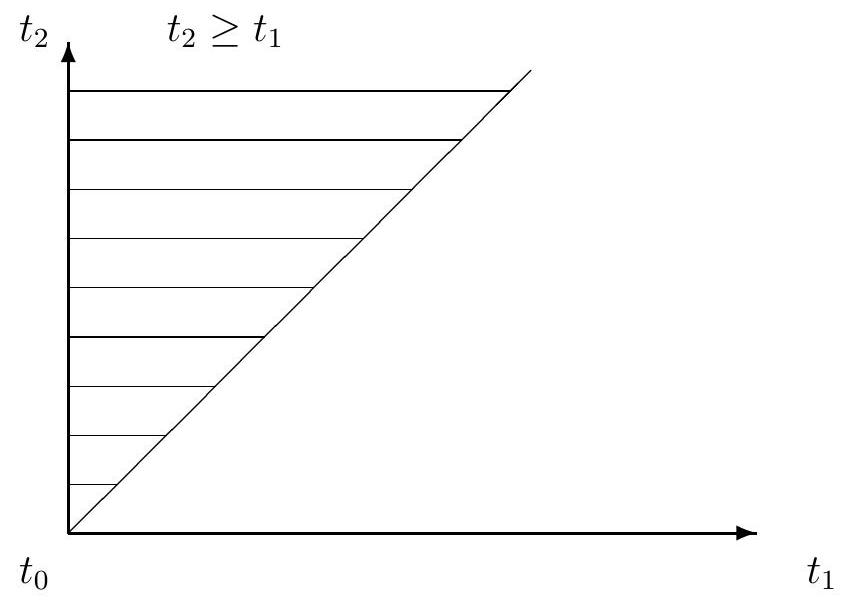
\includegraphics[max width=\textwidth, center]{2025_06_07_f7019c98c95e0473d81eg-03}

\subsubsection*{Zeitordnungs-Operator}
Die Integration über $t_{1}$ und $t_{2}$ etc. in der Neumann'schen Reihe läßt sich durch die Einführung des sog. Zeitordnungsoperators $T$ symmetrisieren. Er ist wie folgt definiert:

$$
T\left(H\left(t_{1}\right) H\left(t_{2}\right)\right) \equiv\left\{\begin{array}{lll}
H\left(t_{1}\right) H\left(t_{2}\right) & \text { für } & t_{1}>t_{2} \\
H\left(t_{2}\right) H\left(t_{1}\right) & \text { für } & t_{2}>t_{1}
\end{array}\right.
$$

Insbesondere gilt $T\left(H\left(t_{1}\right) H\left(t_{2}\right)\right)=T\left(H\left(t_{2}\right) H\left(t_{1}\right)\right)$, und somit

$$
\int_{t_{0}}^{t} d t_{2} H\left(t_{2}\right) \int_{t_{0}}^{t_{2}} d t_{1} H\left(t_{1}\right)=\frac{1}{2} \int_{t_{0}}^{t} \int_{t_{0}}^{t} T\left(H\left(t_{1}\right) H\left(t_{2}\right)\right) d t_{1} d t_{2}
$$

Mit der Stufenfunktion $\theta(t)$,

$$
\theta(t)=\left\{\begin{array}{lll}
1 & \text { für } & t>0 \\
0 & \text { für } & t<0
\end{array}\right.
$$

läßt sich der Zeitordnungsoperator auch als

$$
T\left(H\left(t_{1}\right) H\left(t_{2}\right)\right)=\theta\left(t_{1}-t_{2}\right) H\left(t_{1}\right) H\left(t_{2}\right)+\theta\left(t_{2}-t_{1}\right) H\left(t_{2}\right) H\left(t_{1}\right)
$$

schreiben. Allgemein gilt somit

$$
T\left(H\left(t_{1}\right) \cdots H\left(t_{n}\right)\right)=\sum_{\text {Permut. }} \theta\left(t_{\alpha_{1}}-t_{\alpha_{2}}\right) \cdots \theta\left(t_{\alpha_{n-1}}-t_{\alpha_{n}}\right) H\left(t_{\alpha_{1}}\right) \cdots H\left(t_{\alpha_{n}}\right) .
$$

Der Zeitentwicklungsoperator spielt in allen störungstheoretischen Darstellungen eine fundamentale Rolle, insbesondere auch in der Theorie der Green'schen Funktionen, durch welche alle Meßprosses in der Vielteichlichentheorie dargestellt werden.

\subsubsection*{Formale Darstellung der Neumann-Reihe}
Mit Hilfe des Zeitordnungsoperators $T$ lässt sich die Neumann-Reihe für den Zeitentenwicklungsoperators $U\left(t, t_{0}\right)$ formal wie folgt darstellen:

$$
\begin{aligned}
U\left(t, t_{0}\right) & =\sum_{n=0}^{\infty}\left(\frac{1}{i \hbar}\right)^{n} \frac{1}{n!} \int_{t_{0}}^{t} \cdots \int_{t_{0}}^{t} d t_{1} \cdots d t_{n} T\left(H\left(t_{1}\right) \cdots H\left(t_{n}\right)\right) \\
& \equiv T\left(\exp \left\{-\frac{i}{\hbar} \int_{t_{0}}^{t} d t^{\prime} H\left(t^{\prime}\right)\right\}\right)
\end{aligned}
$$

Diese Darstellung ist formal, da jede praktische Rechnung mit der ursprünglichen Definition durchgeführt werden muss. Für formale Umformungen und die Entwicklung diagramatischer Methoden ist der Zeitordnungsoperator jedoch unerläßlich.

\subsubsection*{Unitarität}
Für zwei allgemeine Lösungen $\psi(t)$ und $\phi(t)$ gilt

$$
i \hbar \frac{d}{d t}(\psi(t), \phi(t))=(\psi(t), H(t) \phi(t))-(H(t) \psi(t), \phi(t))=0
$$

für die zeitliche Entwicklung des Skalarprodukt, da $H(t)$ selbstadjungiert ist. Damit ist also das Skalarprodukt eine Konstante der Bewegung und aus

$$
(\psi(t), \phi(t))=\left(U\left(t, t_{0}\right) \psi\left(t_{0}\right), U\left(t, t_{0}\right) \phi\left(t_{0}\right)\right)=\left(\psi\left(t_{0}\right), \phi\left(t_{0}\right)\right)
$$

folgt das $U\left(t, t_{0}\right)$ unitär ist.

\subsection*{Dirac- oder Wechselwirkungsbild}
Dieses, vor allem für die Störungstheorie wichtige Bild zur zeitlichen Entwicklung eines quantentheoretischen Systems, wurde von Dirac eingeführt (s. Kap. 9.1).

\subsubsection*{Zeitunabhängiges ungestörtes System}
Im Normalfall gilt

$$
H(t)=H_{0}+V(t)
$$

das ungestörte System $H_{0}$ ist also nicht explizit von der Zeit abhängig.

\subsubsection*{Zeitentwicklung durch $H_{0}$}
Beim Wechselwirkungsbild separiert man die Zeitentwicklung von Wellenfunktion im Schrödinger-Bild, $\psi_{S}(t)$ in zwei Anteile. Die Zeitentwicklung durch $H_{0}$ ist durch

$$
\begin{aligned}
\psi_{I}(t) & =e^{i H_{0} t / \hbar} \psi_{S}(t) \\
A_{I}(t) & =e^{i H_{0} t / \hbar} A_{S} e^{-i H_{0} t / \hbar}
\end{aligned}
$$

gegeben. $\psi_{I}(t)$ ist die Wellenfunktion im Wechselwirkungsbild ( $I$ steht für interaction). Ohne Störung ( $V=0$ ) gilt

$$
\psi_{I}(t)=\psi_{S}(t)
$$

Für eine Störung $V(t)$, welche für $|t|>T$ verschwindet, sind also die Anfangs- und Endzustände $\psi_{S}(\mp T)$ durch

$$
\psi_{S}(\mp T)=\psi_{I}(\mp T)
$$

gegeben.

\subsubsection*{Zeitentwicklung durch die Störung}
Die Zeitentwicklung ist im Wechselwirkungsbild durch

$$
\begin{aligned}
i \hbar \frac{d}{d t} \psi_{I} & =-H_{0} e^{i H_{0} t / \hbar} \psi_{S}(t)+e^{i H_{0} t / \hbar} i \hbar \frac{d}{d t} \psi_{S}(t) \\
& =e^{i H_{0} t / \hbar}\left(H(t)-H_{0}\right) \psi_{S}(t) \\
& =e^{i H_{0} t / \hbar} V(t) e^{-i H_{0} t / \hbar} e^{i H_{0} t / \hbar} \psi_{S}(t) \\
& =V_{I}(t) \psi_{I}(t)
\end{aligned}
$$

geben. Zusammen gilt also

$$
\begin{aligned}
i \hbar \partial_{t} \psi_{I} & =V_{I}(t) \psi_{I}(t) \\
\frac{d}{d t} A_{I} & =\frac{i}{\hbar}\left[H_{0}, A_{I}\right]+\left(\partial_{t} A\right)_{I}
\end{aligned}
$$

Das Wechselwirkungsbild erlaubt es damit die unterschiedliche physikalische Bedeutung von $H_{0}$ und der Störung $V(t)$ mathematisch präzise zu erfassen.

\subsubsection*{Zeitentwicklungsoperator $U_{I}\left(t, t_{0}\right)$ im Welchselwirkungsbild}
Von Interesse ist nun der Zeitentwicklungsoperator $U_{I}\left(t, t_{0}\right)$ im Welchselwirkungsbild, welcher via

$$
\psi_{I}(t)=U_{I}\left(t, t_{0}\right) \psi_{I}\left(t_{0}\right) \quad U_{I}\left(t_{0}, t_{0}\right)=1
$$

definiert ist. Falls $V(t)$ nicht explizit von der Zeit abhängt, so gilt (s. Kap. 9.1)

$$
U_{I}\left(t, t_{0}\right)=e^{i H_{0} t / \hbar} e^{-i H t / \hbar} e^{i H t_{0} / \hbar} e^{-i H_{0} t_{0} / \hbar}
$$

Ist $V(t)$ dagegen zeitabhängig, so bemerkt man wieder (wie im Schrödinger-Bild), daß die Differentialgleichung

$$
i \hbar \partial_{t} U_{I}\left(t, t_{0}\right)=V_{I}(t) U_{I}\left(t, t_{0}\right)
$$

zusammen mit der Anfangsbedingung $U_{I}\left(t_{0}, t_{0}\right)=1$ zu der Integralgleichung

$$
U_{I}\left(t, t_{0}\right)=1+\frac{1}{i \hbar} \int_{t_{0}}^{t} d t^{\prime} V_{I}\left(t^{\prime}\right) U_{I}\left(t^{\prime}, t_{0}\right)
$$

äquivalent ist. Diese hat nun wiederum die formale Lösung

$$
\begin{aligned}
U_{I}\left(t, t_{0}\right) & =\sum_{n=0}^{\infty} \frac{1}{n!} \frac{1}{(i \hbar)^{n}} \int_{t_{0}}^{t} d t_{1} \cdots d t_{n} T\left(V_{I}\left(t_{1}\right) \cdots V_{I}\left(t_{n}\right)\right) \\
& =T\left(\exp \left\{-\frac{i}{\hbar} \int_{t_{0}}^{t} d t^{\prime} V_{I}\left(t^{\prime}\right)\right\}\right)
\end{aligned}
$$

Diese Darstellung ist der maßgebliche Ausgangspunkt für störungstheoretische Rechnungen, indem man sukzessive Terme mit $n=1,2,3$ etc. berücksichtigt.

\subsubsection*{3 Übergänge 1. Ordnung}
Liegt zur Zeit $t=t_{0}$ der Zustand $\left|\psi_{I}\left(t_{0}\right)\right\rangle$ vor, so entwickelt sich daraus aufgrund der Störung $V_{I}(t)$ zur Zeit $t$ der Zustand $\left|\psi_{I}(t)\right\rangle=U_{I}\left(t, t_{0}\right)\left|\psi_{I}\left(t_{0}\right)\right\rangle$.

\subsubsection*{Lineare Störungstheorie}
Nimmt man aus der Reihe für $U\left(t, t_{0}\right)$ nur die Terme mit $n=0$ und 1 mit, so folgt:

$$
\left|\psi_{I}(t)\right\rangle=\left|\psi_{I}\left(t_{0}\right)\right\rangle+\frac{1}{i \hbar} \int_{t_{0}}^{t} d t^{\prime} V_{I}\left(t^{\prime}\right)\left|\psi_{I}\left(t_{0}\right)\right\rangle
$$

Die Korrektur ist also linear in der Störung.\\
Eigenzuständen von $H_{0}$\\
Es seien

$$
\left|\varphi_{n}\right\rangle, \quad H_{0}\left|\varphi_{n}\right\rangle=E_{n}\left|\varphi_{n}\right\rangle,
$$

die stationären Eigenzustände von $H_{0}$. Wir wählen einen Eigenzustand als Anfangszustand:

$$
\left|\psi_{I}(-T)\right\rangle=\left|\varphi_{n}\right\rangle, \quad t_{0}=-T, \quad T \gg 0
$$

\subsubsection*{Entwicklung nach Eigenfunktionen von $H_{0}$}
Die Wahrscheinlichkeitsamplitude dafür, daß sich das System zur Zeit $t=+T \mathrm{im}$ Zustand $\left|\varphi_{m}\right\rangle$ befindet, ist durch

$$
\left\langle\varphi_{m} \mid \psi_{I}(T)\right\rangle=\delta_{m n}+\frac{1}{i \hbar} \int_{-T}^{+T} d t^{\prime}\left\langle\varphi_{m}\right| V_{I}\left(t^{\prime}\right)\left|\varphi_{n}\right\rangle
$$

gegeben. Aus $V_{I}(t)=e^{i H_{0} t / \hbar} V(t) e^{-i H_{0} t / \hbar}$, folgt

$$
\left\langle\varphi_{m}\right| V_{I}(t)\left|\varphi_{n}\right\rangle=e^{i\left(E_{m}-E_{n}\right) t / \hbar}\left\langle\varphi_{m}\right| V(t)\left|\varphi_{n}\right\rangle,
$$

und daher

$$
\left\langle\varphi_{m} \mid \psi_{I}(T)\right\rangle=\delta_{m n}+\frac{1}{i \hbar} \int_{-T}^{+T} d t^{\prime} e^{i\left(E_{m}-E_{n}\right) t^{\prime} / \hbar}\left\langle\varphi_{m}\right| V\left(t^{\prime}\right)\left|\varphi_{n}\right\rangle
$$

\subsubsection*{Übergangswahrscheinlichkeit}
Dies ist die grundlegende Formel für die Berechnung der Übergangswahrscheinlichkeit

$$
w_{n \rightarrow m}(2 T)=\left|\left\langle\varphi_{m} \mid \psi_{I}(T)\right\rangle\right|^{2}
$$

für die Störungstheorie in ersten Ordnung in $V(t)$. Um die Formel weiter auszuwerten, sind zusätzliche Kenntnisse zur Form von $V(t)$ notwendig. Zwei wichtige Beispiele werden nun diskutiert.

\subsubsection*{Zeitunabhängiges Potential}
Falls $V$ nicht explizit von der Zeit abhängt, so läßt sich für $\omega_{m n} \neq 0$ das Zeitintegral unmittelbar ausführen:

$$
\int_{-T}^{+T} d t^{\prime} e^{i \omega_{n m} t^{\prime}}=\frac{2 \sin \left(\omega_{m n} T\right)}{\omega_{m n}} \quad \omega_{m n}=\frac{1}{\hbar}\left(E_{m}-E_{n}\right)
$$

\subsubsection*{Darstellung der $\delta$-Funktione}
Bei der Berechnung von $w_{n \rightarrow m}(2 T)$ ist die Darstellung

$$
\lim _{T \rightarrow \infty}\left(\frac{\sin ^{2}(x T)}{\pi x^{2} T}\right)=\delta(x)
$$

für die Distribution $\delta(x)$ nützlich. Begründung: Es sei $f(x)$ eine Testfunktion. Dann gilt

$$
\int_{-a}^{+a} d x \frac{\sin ^{2}(x T)}{x^{2} T} f(x)=\int_{-a T}^{+a T} d y \frac{\sin ^{2}(y)}{y^{2}} f(y / T), \quad y=T x
$$

Für große $T$ folgt daraus

$$
\int_{-a}^{+a} d x \frac{\sin ^{2}(x T)}{x^{2} T} f(x) \approx f(0) \int_{-\infty}^{+\infty} d y \frac{\sin ^{2}(y)}{y^{2}}=f(0) \pi
$$

\subsubsection*{Übergangswahrscheinlichkeit}
Für $E_{m} \neq E_{n}$ und $T \rightarrow \infty$ erhalten wir somit

$$
\begin{aligned}
w_{n \rightarrow m}(2 T) & \left.=\left|\frac{2 \sin \left(\omega_{m n} T\right)}{i \hbar \omega_{m n}}\right|^{2}\left|\left\langle\varphi_{m}\right| V\right| \varphi_{n}\right\rangle\left.\right|^{2} \\
& \left.=\frac{4 \pi T}{\hbar^{2}} \delta\left(\omega_{m n}\right)\left|\left\langle\varphi_{m}\right| V\right| \varphi_{n}\right\rangle\left.\right|^{2}
\end{aligned}
$$

für die Übergangswahrscheinlichkeit. Wegen $\delta(a x)=\frac{1}{|a|} \delta(x)$ bekommen wir damit für die Übergangsrate

$$
\Gamma_{n \rightarrow m}=w_{n \rightarrow m}(2 T) /(2 T)
$$

das wichtige Resultat

$$
\left.\Gamma_{n \rightarrow m}=\frac{2 \pi}{\hbar} \delta\left(E_{n}-E_{m}\right)\left|\left\langle\varphi_{m}\right| V\right| \varphi_{n}\right\rangle\left.\right|^{2}
$$

\subsubsection*{Fermi's goldene Regel}
$\overline{\mathrm{Im}}$ allgemeinen steht als Endzustand nicht nur ein einziger Zustand $\varphi_{m}$ mit scharfer Energie experimentell zur Verfügung, sondern ein Energieintervall $\Delta E_{m}$, in dem $\rho\left(E_{m}\right) \Delta\left(E_{m}\right)$ Zustände liegen. Dann beträgt die Gesamtrate

$$
\left.\bar{\Gamma}_{n}\left(E_{n}\right)=\int d E_{m} \rho\left(E_{m}\right) \Gamma_{n \rightarrow m}=\frac{2 \pi}{\hbar} \rho\left(E_{n}\right)\left|\left\langle\varphi_{n}\right| V\right| \varphi_{n}\right\rangle\left.\right|^{2}
$$

Diese Formel wird (nach Fermi) als Goldene Regel der zeitabhängige Störungstheorie 1. Ordnung bezeichnet.

\begin{itemize}
  \item Es sei betont, daß die 1. Ordnung der Störungstheorie nur Sinn macht, falls die höheren Ordnungen entsprechend vernachlässigt werden können.
  \item Die Zustandsdichte $\rho\left(E_{n}\right)$ läßt sich experimentell mittels der goldenen Regel bestimmen wenn die Matrixelmente $\left\langle\varphi_{n}\right| V\left|\varphi_{n}\right\rangle$ nur schwach von der Energie $E_{n}$ abhängig sind.
\end{itemize}

\subsubsection*{Zeitlich periodisches Potential}
$V(t)$ habe die Gestalt

$$
V(t)=A e^{-i \omega t}+A^{+} e^{i \omega t}
$$

wobei $A$ eine beliebiger Operator ist. Damit ist $V(t)$ selbstadjungiert und periodisch in der Zeit $t$.

\subsubsection*{Übergangsamplitude}
Für die Übergangsamplitude ergibt sich daraus

$$
\left\langle\varphi_{m} \mid \varphi_{I}(T)\right\rangle=\frac{1}{i \hbar} \int_{-T}^{+T} d t\left[e^{i\left(\omega_{m n}-\omega\right) t}\langle m| A|n\rangle+e^{i\left(\omega_{m n}+\omega\right) t}\langle m| A^{+}|n\rangle\right]
$$

Bei der Berechnung der Übergangswahrscheinlichkeit ist zu beachten, daß die gemischten Terme beim Quadrieren wegfallen: Für sehr große $T$ gilt nämlich für $m \neq n$

$$
\int_{-T}^{+T} d t e^{i\left(\omega_{m n}-\omega\right) t} \int_{-T}^{+T} d t^{\prime} e^{i\left(\omega_{m n}+\omega\right) t^{\prime}} \approx \delta\left(\omega_{m n}-\omega\right) \delta\left(\omega_{m n}+\omega\right)=0
$$

Wir haben demnach für große $T$

$$
\left.\left.w_{n \rightarrow m}=\left.4 \pi T \frac{1}{\hbar^{2}}\left[\delta\left(\omega_{m n}-\omega\right)|\langle m| A| n\right\rangle\right|^{2}+\delta\left(\omega_{m n}+\omega\right)\left|\langle m| A^{+}\right| n\right\rangle\left.\right|^{2}\right]
$$

\subsubsection*{Emission und Absorption}
Für die Rate $\Gamma_{n \rightarrow m}=w_{m \rightarrow n} /(2 T)$ folgt hieraus

$$
\left.\left.\Gamma_{n \rightarrow m}=\left.\frac{2 \pi}{\hbar}\left[\delta\left(E_{m}-E_{n}-\hbar \omega\right)|\langle m| A| n\right\rangle\right|^{2}+\delta\left(E_{m}-E_{n}+\hbar \omega\right)\left|\langle m| A^{+}\right| n\right\rangle\left.\right|^{2}\right]
$$

Wegen $E_{m}=E_{n}+\hbar \omega$ beschreibt der Operator $A$ einen Absorptionsproze $\beta$, während $A^{+}$ wegen $E_{m}=E_{n}-\hbar \omega$ einen Emissionsprozeß für ein Quant der Energie $\hbar \omega$ beschreibt.

\subsubsection*{Photonen}
Die gerade skizzierten Überlegungen sind die Grundlage für das Verständnis von Absorption und Emission von Strahlung. Dabei sind dann die $A^{+}$und $A$ die Erzeugungs- und Vernichtungsoperatoren für Lichtquanten, den Photonen. Allerdings kommt zu $V(t)$ dann auch noch die Ortsabhängigkeit der ebenen Wellen, $\sim \exp (i \mathbf{k} \cdot \mathbf{x})$ hinzu.

\subsection*{Potentialstreuung: 1. Ordnung Störungstheorie}
Es sei $H_{0}=-\frac{\hbar^{2}}{2 m} \Delta$ und $\tilde{V}$ ein Potential, an dem die im Anfangs- und Endzustand freien Teilchen gestreut werden, $H=H_{0}+\tilde{V}$.\\
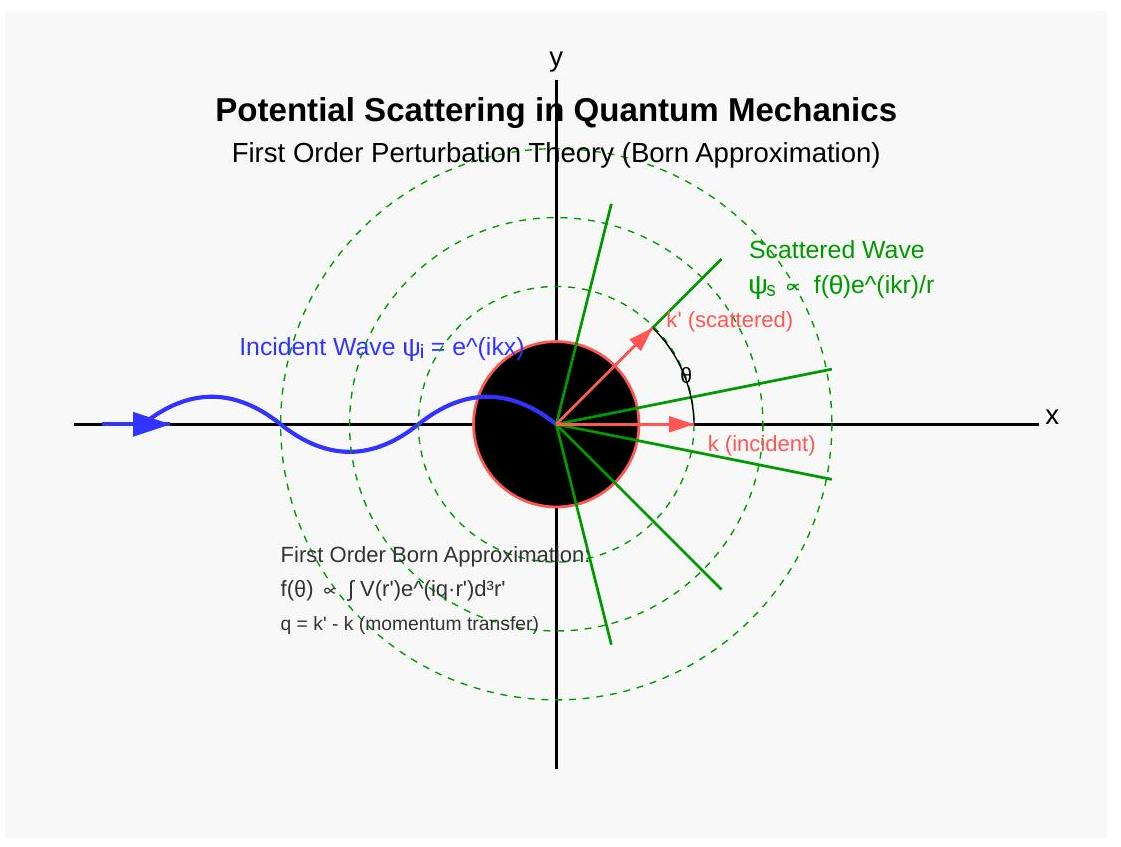
\includegraphics[max width=\textwidth, center]{2025_06_07_f7019c98c95e0473d81eg-10}

Figure 10.1: Potentialstreuung Illustration

\subsubsection*{Periodische Randbedingungen}
Das System sei in einem Volumen $V=L^{3}$ gegeben. Als Basis wählen wir die freien Wellenfunktionen

$$
\varphi_{\vec{k}}=\frac{1}{\sqrt{V}} e^{i \vec{k} \cdot \vec{x}}
$$

Da wir am Limes $V \rightarrow \infty$ interesiert sind, können wir die Randbedingungen frei wählen. Günstig sind die periodischen Randbedingungen:

$$
e^{i k_{j} L}=1, \quad \vec{k}=\frac{2 \pi}{L} \vec{n}, \quad \vec{n}=\left(n_{1}, n_{2}, n_{3}\right), \quad n_{i}=0, \pm 1, \pm 2, \ldots
$$

\subsubsection*{Anfangs- und Endzustand}
Wir betrachten einen Streuprozess an einem räumlich begrenzten Potential $\tilde{V}$. Dann sind sowohl der Anfangs- wie auch der Endzustand ebene Wellen:

$$
\begin{array}{lll}
\text { Anfangszustand: } & \varphi_{\vec{k}_{a}}=\frac{1}{\sqrt{V}} e^{i \vec{k}_{a} \cdot \vec{x}} & E_{a}=\frac{\hbar^{2} k_{a}^{2}}{2 m} \\
\text { Endzustand: } & \varphi_{\vec{k}_{e}}=\frac{1}{\sqrt{V}} e^{i \vec{k}_{e} \cdot \vec{x}} & E_{e}=\frac{\hbar^{2} k_{e}^{2}}{2 m}
\end{array}
$$

\subsubsection*{Goldene Regel}
Für die Übergangsrate $\Gamma_{\vec{k}_{a} \rightarrow \vec{k}_{e}}$ erhält man nach der Goldene Regel

$$
\left.\Gamma_{\vec{k}_{a} \rightarrow \vec{k}_{e}}=\frac{2 \pi}{\hbar} \delta\left(E_{e}-E_{a}\right)\left|\left\langle\vec{k}_{e}\right| \tilde{V}\right| \vec{k}_{a}\right\rangle\left.\right|^{2}
$$

mit

$$
\left.\left|\left\langle\vec{k}_{e}\right| \tilde{V}\right| \vec{k}_{a}\right\rangle\left.\right|^{2}=\frac{1}{V} \int d^{3} x e^{i\left(\vec{k}_{a}-\vec{k}_{e}\right) \cdot \vec{x}} \tilde{V}(\vec{x})
$$

Die Anzahl der Zustände im Endzustandsintervall $\Delta k_{1 e} \Delta k_{2 e} \Delta k_{3 e}=\Delta^{3} k_{e}$ ist durch

$$
\Delta^{3} n_{e}=\frac{V}{(2 \pi)^{3}} \Delta^{3} k_{e}
$$

gegeben. Die zugehörige Rate ist demnach

$$
\Gamma_{\vec{k}_{a} \rightarrow \vec{k}_{e}} \Delta^{3} n_{e}=\frac{1}{(2 \pi)^{2} \hbar V} \delta\left(E_{a}-E_{e}\right) \Delta^{3} k_{e}\left|\int d^{3} x e^{i\left(\vec{k}_{a}-\vec{k}_{e}\right) \cdot \vec{x}} \tilde{V}(\vec{x})\right|^{2}
$$

\subsubsection*{Teilchenstromdichte}
Die Teilchenstromdichte $\vec{j}_{a}$ der einfallenden Teilchen ist

$$
\vec{j}_{a}=\frac{1}{V} \frac{\hbar \vec{k}_{a}}{m}
$$

Damit erhalten wir für den 3-fach differentiellen Wirkungsquerschnitt $\Delta \sigma=j_{e} \Delta \Omega_{e} / j_{a}$

$$
\Delta \sigma=\frac{\Gamma_{\vec{k}_{a} \rightarrow \vec{k}_{e}} \Delta^{3} n_{e}}{\left|\vec{j}_{a}\right|}=\frac{m}{(2 \pi \hbar)^{2}} \frac{1}{\left|\vec{k}_{a}\right|} \delta\left(E_{a}-E_{e}\right) \Delta^{3} k_{e}\left|\int d^{3} x e^{i\left(\vec{k}_{a}-\vec{k}_{e}\right) \cdot \vec{x}} \tilde{V}(\vec{x})\right|^{2}
$$

Wegen

$$
\Delta^{3} k_{e}=k_{e}^{2} d k_{e} d \Omega_{e}=\frac{m}{\hbar^{2}} k_{e} d E_{e} d \Omega_{e}
$$

bekommen wir schließlich mit $k_{e}=k_{a}$

$$
\Delta \sigma=\frac{m^{2}}{\left(2 \pi \hbar^{2}\right)^{2}}\left|\int d^{3} x e^{i\left(\vec{k}_{a}-\vec{k}_{e}\right) \cdot \vec{x}} \tilde{V}(\vec{x})\right|^{2} \delta\left(E_{a}-E_{e}\right) d E_{e} d \Omega_{e}
$$

\subsubsection*{Differentielle Wirkungsquerschnitt}
Die Integration über die Endzustandsenergie $E_{e}$ ergibt die wichtige Formel

$$
\frac{d \sigma^{(1)}}{d \Omega_{e}}=\frac{m^{2}}{\left(2 \pi \hbar^{2}\right)^{2}}\left|\int d^{3} x e^{i\left(\vec{k}_{a}-\vec{k}_{e}\right) \cdot \vec{x}} \tilde{V}(\vec{x})\right|^{2}
$$

(Der Index (1) soll andeuten, daß es sich lediglich um die 1. Näherung handelt.)

\subsubsection*{Impulsübertrag}
Man sieht, daß $d \sigma^{(1)} / d \Omega_{e}$ nur vom Impulsübertrag $\vec{q}=\vec{k}_{a}-\vec{k}_{e}$ abhängt.

Falls $\tilde{V}(\vec{x})=\tilde{V}(r)$, so läßt sich das Integral noch weiter vereinfachen:

$$
\begin{aligned}
\int d^{3} x e^{i r q \cos \theta} \tilde{V}(r) & =2 \pi \int_{0}^{\infty} d r r^{2} \tilde{V}(r) \int_{0}^{\pi} d \theta e^{i r q \cos \theta} \sin \theta \\
& =2 \pi \int_{0}^{\infty} d r r^{2} \tilde{V}(r) \int_{-1}^{+1} d z e^{i r q z} \\
& =\frac{4 \pi}{q} \int_{0}^{\infty} d r r \tilde{V}(r) \sin (q r)
\end{aligned}
$$

so daß

$$
\frac{d \sigma^{(1)}}{d \Omega_{e}}=\left(\frac{4 m^{2}}{q^{2} \hbar^{4}}\right)\left|\int_{0}^{\infty} d r r \tilde{V}(r) \sin (q r)\right|^{2}
$$

\subsubsection*{Yukawa-Potential}
Das abgeschirmte Coulomb-Potential

$$
\tilde{V}(r)=g \frac{e^{-\mu r}}{r}
$$

wird auch das Yukawa-Potential genannt, hierbei ist $1 / \mu$ die Abschirmlänge.\\
Da $\int_{0}^{\infty} d r e^{-\mu r} \sin (r q)=\frac{q}{q^{2}+\mu^{2}}$, so folgt

$$
\frac{d \sigma^{(1)}}{d \Omega_{e}}=\left(\frac{2 m g}{\hbar^{2}}\right)^{2} \frac{1}{\left(q^{2}+\mu^{2}\right)^{2}}
$$

Da

$$
\begin{gathered}
\vec{q}^{2}=\left(\vec{k}_{a}-\vec{k}_{e}\right)^{2}=2 k_{a}^{2}\left(1-\cos \left[\angle\left(\vec{k}_{a}, \vec{k}_{e}\right)\right]\right), \\
\angle\left(\vec{k}_{a}, \vec{k}_{e}\right)=\vartheta: \quad \text { Streuwinkel },
\end{gathered}
$$

und $(1-\cos \vartheta)=2 \sin ^{2}(\vartheta / 2)$, so folgt

$$
q^{2}=4 k_{a}^{2} \sin ^{2} \frac{\vartheta}{2}=\frac{8 m E_{a}}{\hbar^{2}} \sin ^{2} \frac{\vartheta}{2}
$$

\subsubsection*{Rutherford'sche Streuformel}
Für $\mu=0$ ergibt sich daher

$$
\frac{d \sigma^{(1)}}{d \Omega}=\frac{g^{2}}{16 E_{a}^{2}} \frac{1}{\sin ^{4} \frac{\vartheta}{2}}
$$

Dies ist die Rutherford'sche Formel für die Coulomb-Streuung. Sie ergibt sich also quantenmechanisch in 1. Ordnung Störungstheorie.

\end{document}